\documentclass[licencjacka]{pracamgr_Kogni}

\usepackage{kotex} % Korean typesetting package
\usepackage{polski}
\usepackage{natbib} % bibliografia
\usepackage{enumitem} % numerowanie
\usepackage{setspace} % ustawienie interlinii
\usepackage{xurl} % rozdzielanie url
\usepackage[table]{xcolor} % kolor w~tabelach
\usepackage{arydshln} % przerywane linie
\usepackage{tikz-dependency} % drzewa
\usepackage{stmaryrd} % rysunki do drzew
\usepackage{gb4e} % przykłady
\usepackage{hyperref} % referencje i~url
\usepackage{graphicx} % pdfy
\usepackage{float} % ruszanie obrazkow
\usepackage{textcomp} % matematyczne minusy
\usepackage{rotating} % obracanie wykresów
\usepackage{amssymb} % \square
\usepackage{multicol} % kolumny 
\usepackage[bottom]{footmisc} % stopki
\usepackage{tablefootnote} % przypisy w~tabelach
\usepackage{array}
\usepackage{amsmath} % odnośniki z nawiasami
\usepackage{booktabs} % tabelki
\usepackage{multirow} % scalanie komórek w~pionie
\usepackage{microtype}
\usepackage[T1]{fontenc}
\usepackage{lmodern}
\usepackage{adjustbox}
\usepackage{float} % wymusza lokalizację tabel\\
\usepackage{amsmath} % ułamki
\usepackage{underscore}
\usepackage{tikz}
\usepackage{xpatch}
\usepackage{xparse}
\usepackage{metrix} % skandowanie tekstu
\usepackage{placeins} % blokowanie latających tabel


\hypersetup{
     colorlinks=true,
     linkcolor=black,
     citecolor=black,
     urlcolor=black,
     }
     
\makeatletter
\def\namedlabel#1#2{\begingroup
    #2%
    \def\@currentlabel{#2}%
    \phantomsection\label{#1}\endgroup
}
\makeatother

\onehalfspacing{
\counterwithout{footnote}{chapter}
\autor{Wojciech Stempniak}{433855}
\title{Struktura zależnościowa koordynacji --~analiza korpusów Universal~Dependencies}
\kierunek{kognitywistyka}
\opiekun{prof. dr.~hab. Adama Przepiórkowskiego\\
Uniwersytet Warszawski}
\date{czerwiec 2024}
\keywords{koordynacja, struktura koordynacji, zależności składniowe, drzewa zależnościowe, Universal Dependencies (UD), Dependency Length Minimization (DLM), języki inicjalne, języki finalne, badanie korpusowe}

\begin{document}

\maketitle

    \tytulang{Dependency structure of coordination -- an analysis of Universal Dependencies corpora}

    \begin{abstract}{
Istnieje wiele poglądów na temat struktury zależnościowej koordynacji, czyli konstrukcji współrzędnie złożonej. W~literaturze opisane są cztery główne podejścia -- model praski, londyński, stanfordzki i~moskiewski \citep{popel2013coordination}.

Poprzednie badania \citep{przepiorkowski2023conjunct} opisują metodę pozwalającą na testowanie poprawności tych modeli. Polega ona na analizie tendencji do umieszczania krótszego członu koordynacji na początku konstrukcji współrzędnie złożonej. Wykorzystuje ona zasadę Dependency Length Minimization (DLM, \citealt{temperley2007minimization}), czyli tendencję do formułowania zdań tak, aby łączna długość relacji między słowami w~zdaniu była jak najmniejsza. \cite{przepiorkowski2023conjunct} na podstawie analizy koordynacji w~korpusie języka angielskiego argumentują za poprawnością modeli symetrycznych, czyli podejścia praskiego i~londyńskiego.

Cztery główne modele struktury zależnościowej koordynacji zostały opracowane na podstawie analiz języków inicjalnych, czyli takich, w~których głowy znajdują się zwykle na początku fraz. Jednak podejścia te mogą nie opisywać prawidłowo koordynacji w~językach finalnych, tj. takich, w~których głowa zwykle jest na końcu frazy. \cite{kanayama2018coordinate} postulują wprowadzenie alternatywnych modeli struktury zależnościowej koordynacji dla języków finalnych. W~niniejszej pracy przedstawiam przewidywania 12 modeli struktury zależnościowej koordynacji. Zestawiam je z~wynikami analizy korpusów językowych opisanych w~standardzie Universal Dependencies (UD, \citealt{de2021universal}). W~badaniu uwzględniono korpusy 13 języków, w~tym 9 inicjalnych i~2 finalnych.

Wyniki badania potwierdzają występowanie w~języku angielskim tendencji zaobserwowanych w~pracy \cite{przepiorkowski2023conjunct}. Podobne zależności występują także w~języku czeskim oraz w~łacinie. Niemniej jednak w~pozostałych badanych językach przewidywane tendencje nie zostały zaobserwowane. Pokazuję, że może to wynikać z~niewystarczającej ilości oraz złej jakości danych użytych w~badaniu. Proponuję poprawę metodologii i~dalsze badania dotyczące struktury zależnościowej koordynacji.
}
    \end{abstract}

    \thispagestyle{empty}
    \setcounter{page}{3}

\chapter*{Podziękowania}

Pragnę złożyć serdeczne podziękowania mojemu promotorowi prof. dr. hab. Adamowi Przepiórkowskiemu za inspirację i~pomoc w~prowadzeniu badań oraz cierpliwość, wyrozumiałość i~zaangażowanie podczas kierowania moją pracą.

Ukończenie niniejszej pracy nie~byłoby możliwe bez pomocy mgr. Berkego \c{S}en\c{s}ekerci, któremu serdecznie dziękuję za pomoc w~dostosowaniu stosowanych przeze mnie algorytmów do~warunków języków finalnych i~ewaluacji algorytmu użytego do analizy języka tureckiego.

Dziękuję również Magdalenie Borysiak, Katarzynie Zrobek i~Oskarowi Pruszyńskiemu za~koleżeńską pomoc w~prowadzeniu badań i~zgłębianiu wiedzy na temat badanych przeze mnie zjawisk.
    
    \tableofcontents % Tytuł, streszczenie i podziękowania

%\chapter{Wprowadzenie} \label{ch1}
\section{Cel pracy}

Jedno z~pytań, na które próbuje odpowiedzieć teoria składni, brzmi: ,,Dlaczego układamy słowa w~zdaniach w~ten sposób, a nie inaczej?''

Rozważmy dwa zdania:

\begin{exe}
\ex \label{gazeta+książka} Wczoraj \emph{czytałem} [[gazetę] i~[bardzo ciekawą książkę przygodową]].
\ex \label{książka+gazeta} Wczoraj \emph{czytałem} [[bardzo ciekawą książkę przygodową] i~[gazetę]].
\end{exe}

W~zdaniach \eqref{gazeta+książka} i~\eqref{książka+gazeta} znajdują się koordynacje zawierające dwa człony: \emph{gazetę} oraz \emph{bardzo ciekawą książkę przygodową}. Jedyną różnicą między tymi zdaniami jest kolejność ustawienia tych członów. Człony mają podobne własności syntaktyczne i~semantyczne. W~związku z~tym można by przypuszczać, że nie ma znaczenia, który człon zostanie umieszczony w~zdaniu jako pierwszy. Niemniej jednak człony różnią się długością. Długość członu można liczyć na rozmaite sposoby -- w~słowach, tokenach, sylabach lub znakach. Na przykład, \emph{bardzo ciekawą książkę przygodową} ma 4~tokeny i~33 znaki, zaś \emph{gazetę} ma 1 token i~6 znaków. 


Pierwszą rzeczą, jaką wykazuję, jest to, że długość członów koordynacji jest istotnym czynnikiem w~wyborze ich kolejności. Wynika to ze zjawiska znanego jako Dependency Length Minimization (DLM). Jest to uniwersalna zależność występująca w~języku naturalnym. Polega ona na tym, że słowa układane są w~zdania w~sposób minimalizujący sumę długości relacji składniowych między nimi \citep{temperley2007minimization, futrell2015large}. Ponieważ długość relacji wewnątrz członów koordynacji jest stała, jedynie ustawienie członów w~zdaniu ma wpływ na sumę długości relacji. 
W~tej pracy badam, w~jaki sposób pozycja nadrzędnika wpływa na ustawienie kolejności członów. Pokazuję, że~w~językach inicjalnych, takich jak polski czy angielski, zdanie o strukturze takiej jak \eqref{gazeta+książka} ma większą szansę na pojawienie się w~języku naturalnym niż zdanie takie, jak \eqref{książka+gazeta}.

Drugim problemem, jaki podejmuję, jest kwestia opisu relacji składniowych. Wśród lingwistów nie ma zgody co do tego, jakie dokładnie relacje zależnościowe łączą poszczególne elementy koordynacji. Istnieją cztery uznawane sposoby opisu -- model praski, londyński, stanfordzki i~moskiewski \citep{popel2013coordination, przepiorkowski2023conjunct}. Niemniej jednak, zakładając prawdziwość DLM, można wykazać, że nie wszystkie podejścia są poprawne. W~tej pracy sprawdzam, które modele tworzą drzewa zależnościowe zgodne z~przewidywaniami DLM.

\cite{przepiorkowski2023conjunct} przeprowadzili analizę koordynacji w~języku angielskim. Wykazali, że modele stanfordzki i~moskiewski nie są poprawnymi metodami opisu koordynacji. Moim głównym celem jest replikacja tego badania oraz rozszerzenie go na trzynaście języków. W~ramach badania analizuję koordynacje osobno w~językach inicjalnych oraz finalnych.

W badaniu wykorzystuję korpusy zależnościowe opisane w wersji 2.14 standardu Universal Dependencies \citep{de2021universal}. Korpusy te pochodzą ze strony \url{https://universaldependencies.org/}. 
Wszystkie skrypty użyte w analizie dostępne są w~repozytorium pod adresem \url{https://github.com/wjstempniak/Dependency-Structure-of-Coordination}.

\section{Struktura pracy}

Niniejszy pierwszy rozdział pracy poświęcam wprowadzeniu do tematu i~opisaniu struktury pracy. W~rozdziale~\ref{ch2}. przedstawiam podstawy teoretyczne mojej pracy. Przedstawiam dokładnie problem opisywania struktury koordynacji i~omawiam standard Universal Dependencies~(UD). W~rozdziale~\ref{ch3}. przedstawiam przewidywania różnych modeli dotyczących struktury koordynacji w~językach inicjalnych i~finalnych. W~rozdziale~\ref{ch4}. przedstawiam kolejne etapy przeprowadzonego przeze mnie badania. Szczególną uwagę poświęcam problemowi automatycznego wyznaczania granic członów koordynacji. W~rozdziale~\ref{ch5}. opisuję analizę statystyczną uzyskanych przeze mnie wyników. W~rozdziale~\ref{ch6}. przedstawiam wnioski wyciągnięte z~badania. Pracę kończę rozdziałem~\ref{ch7}., w~którym opisuję ograniczenia mojej pracy oraz proponuję dalsze możliwości badań w~tej dziedzinie.
 % Wprowadzenie
%\chapter{Wstęp teoretyczny} \label{ch2}
\section{Zależności składniowe}

Zależności składniowe są centralnym zagadnieniem gramatyki zależnościowej, czyli dziedziny teorii składni zajmującej się połączeniami pomiędzy poszczególnymi słowami wchodzącymi w~skład zdania. Są to relacje łączące dwa elementy: nadrzędnik oraz zależny od niego podrzędnik. Elementami łączonymi przez zależności są tokeny -- przez to pojęcie należy rozumieć słowa oraz znaki interpunkcyjne, a także, według niektórych podejść, części niektórych słów.

Relacje występujące w~obrębie zdania można opisać za pomocą grafu zwanego drzewem zależnościowym. \eqref{róża-drzewo} jest przykładowym drzewem zależnościowym zdania \eqref{róża}:

\begin{exe}
\ex \label{róża} W~ręku trzymałam czerwoną różę.\\ 
\ex \label{róża-drzewo}
\begin{dependency}[theme = simple, baseline=-\the\dimexpr\fontdimen22\textfont2\relax]
\begin{deptext}[column sep=1em]
W~\& ręku \& trzymał \& am \& czerwoną \& różę \& .  \\ 
\end{deptext}
\depedge{1}{2}{}
\depedge{3}{1}{}
\deproot{3}{}
\depedge{3}{4}{}
\depedge{6}{5}{}
\depedge{3}{6}{}
\depedge{3}{7}{}
\end{dependency}
\end{exe}

Warto zauważyć, że słowo \emph{trzymałam} składa się z~dwóch tokenów -- \emph{trzymał} oraz \emph{am}.

Należy odróżnić zależności składniowe od relacji składnikowych. Relacje składnikowe łączą poszczególne słowa we~frazy oraz frazy w~bardziej złożone frazy w~zdania \citep{chomsky1956three}.
Schemat \eqref{róża-frazy} przedstawia drzewo zależnościowe zdania \eqref{róża} z~wyróżnionymi niektórymi frazami.

\begin{exe}
\ex \label{róża-frazy}
\begin{dependency}[theme=simple, baseline=-\the\dimexpr\fontdimen22\textfont2\relax]
\begin{deptext}[column sep=1em]
\textbf{W} \& ręku \& trzymał \& am \& czerwoną \& \textbf{różę} \& .  \\ 
\end{deptext}
\depedge{1}{2}{}
\depedge{3}{1}{}
\deproot{3}{}
\depedge{3}{4}{}
\depedge{6}{5}{}
\depedge{3}{6}{}
\depedge{3}{7}{}
\wordgroup{1}{1}{2}{P1}
\wordgroup{1}{5}{6}{P2}
\end{dependency}
\end{exe}

Słowo określające kategorię syntaktyczną danej frazy nazywane jest głową tej frazy \citep{hoeksema1992head}. Przykładowo, głową frazy przyimkowej \emph{W~ręku} jest przyimek \emph{W}, zaś głową frazy rzeczownikowej \emph{czerwoną różę} -- rzeczownik \emph{różę}. 
% Może więcej o kryteriach bycia głową?

W~drzewie zależnościowym głowę danej frazy można rozpoznać po tym, że nie posiada nadrzędników w~jej obrębie.

\section{Universal Dependencies}

Obecnie nie ma w~lingwistyce jednej, szeroko akceptowanej formuły opisu relacji zależnościowych. Standardem, z~którego korzystam, jest Universal Dependencies. Jest to formalizm tworzący ,,ramy dla spójnego opisu gramatyki'' \citep{de2021universal} języków, a więc takich cech jak części mowy, cechy morfologiczne czy właśnie relacje składniowe. 

Universal Dependencies opisuje zależności składniowe za pomocą zestawu uniwersalnych znaczników, charakterystycznych dla rodzaju relacji. Na przykład, relację łączącą podmiot nominalny z~orzeczeniem opisuje znacznik \emph{nsubj}, a dopełnienie bliższe -- \emph{obj}. Znaczniki UD posiadają różne warianty. Podmiot zdania w~trybie biernym opisuje znacznik \emph{nsubj:pass}. W~tej pracy traktuję każdy wariant jako osobny znacznik, chyba że zaznaczam inaczej.

Poniżej znajduje się drzewo zależnościowe zdania \eqref{róża} opisane według standardu~UD.\footnote{Drzewa zależnościowe w~formacie UD wszystkich zdań niepochodzących z~korpusów zostały stworzone przez automatyczne parsowanie parserem Trankit \citep{van2021trankit}.}

\begin{exe}
\ex \label{róża-UD}
\begin{dependency}[baseline=-\the\dimexpr\fontdimen22\textfont2\relax]
\begin{deptext}[column sep=1em]
W~\& ręku \& trzymał \& am \& czerwoną \& różę \& .  \\ 
\end{deptext}
\depedge{2}{1}{case}
\depedge{3}{2}{obl}
\deproot{3}{root}
\depedge{3}{4}{aux:clitic}
\depedge{6}{5}{amod}
\depedge{3}{6}{obj}
\depedge{3}{7}{punct}
\end{dependency}
\end{exe}

Należy zwrócić uwagę na krawędzie łączące tokeny \emph{W}, \emph{ręku} oraz \emph{trzymał}. Według Universal Dependencies głową frazy przyimkowej \emph{W~ręku} jest rzeczownik \emph{ręku}. Jest to sprzeczne z~teorią lingwistyczną i~wskazuje na niedoskonałość tego standardu. Niemniej jednak w~niniejszej pracy będę zakładał poprawność UD.

\section{Koordynacja}

Koordynacja lub konstrukcja współrzędnie złożona to zestawienie w~zdaniu dwóch lub więcej elementów pełniących tę samą funkcję syntaktyczną. Elementy te nazywa się członami koordynacji.

Problem wyznaczania granic członów jest jednym z~ważniejszych aspektów analizy koordynacji. Nie jest to zadanie trywialne i~często wymaga odwołania się do semantyki. Rozważmy następujące przykłady:

\begin{exe}
\ex \label{dzieci+nauczyciele} Niesforne dzieci i~nauczyciele pojechali na wycieczkę.
\ex \label{uczniowie+nauczyciele} Niesforni uczniowie i~nauczyciele pojechali na wycieczkę.
\end{exe}

W~przypadku zdania \eqref{dzieci+nauczyciele} słowo \emph{Niesforne} jest niekontrowersyjnym podrzędnikiem słowa \emph{dzieci}, ponieważ wynika to ze związku zgody.  Z~tego wynika, że granice członów koordynacji wyglądają następująco:
% poprawić: powt. wynika

\begin{exe}
\ex \label{dzieci+nauczyciele-nawiasy}
{[[Niesforne dzieci] i~[nauczyciele]] \emph{pojechali} na wycieczkę.}
\end{exe}

W~zdaniu \eqref{uczniowie+nauczyciele} \emph{Niesforni} może opisywać zarówno \emph{uczniowie}, jak i~\emph{nauczyciele}. W~takim wypadku syntaktyka dopuszcza dwie interpretacje zdania:

\begin{exe}
\ex \label{uczniowie+nauczyciele-dobrze}
{[[Niesforni uczniowie] i~[nauczyciele]] \emph{pojechali} na wycieczkę.}
\ex \label{uczniowie+nauczyciele-źle}
{[Niesforni [[uczniowie] i~[nauczyciele]]] \emph{pojechali} na wycieczkę.}
\end{exe}

W~tej sytuacji prawdopodobne granice członów można wyznaczyć jedynie odwołując się do znaczeń poszczególnych słów. Zdroworozsądkowa semantyka nakazuje nam przyjąć interpretację \eqref{uczniowie+nauczyciele-dobrze}. Poniżej znajduje się drzewo zależnościowe zdania \eqref{uczniowie+nauczyciele} w interpretacji \eqref{uczniowie+nauczyciele-dobrze}, opisane w~standardzie UD, z~zaznaczonymi istotnymi elementami koordynacji.

\begin{exe}
\ex \label{uczniowie+nauczyciele-UD}
\resizebox{\linewidth}{!}{
\begin{dependency}[baseline=-\the\dimexpr\fontdimen22\textfont2\relax]
\begin{deptext}[column sep=.5cm]
Niesforni  \& \textbf{uczniowie} \& i~\& \textbf{nauczyciele} \& \emph{pojechali} \& na \& wycieczkę \& .\\
\end{deptext}
\deproot{5}{root}
\depedge{2}{1}{amod}
\depedge{5}{2}{nsubj}
\depedge{2}{4}{conj}
\depedge{4}{3}{cc}
\depedge{5}{8}{punct}
\depedge{5}{7}{obl}
\depedge{7}{6}{case}
\wordgroup{1}{1}{2}{L}
\wordgroup{1}{4}{4}{R}
\end{dependency}
}
\end{exe}

Człony koordynacji często połączone są spójnikami. Przez spójnik koordynacji rozumiem właśnie ten spójnik, który łączy jej człony. Zakładam, że każda konstrukcja współrzędnie złożona ma co najwyżej jeden spójnik. W~przypadku zdań \eqref{dzieci+nauczyciele} i~\eqref{uczniowie+nauczyciele} jest to~\emph{i}.

Przez lewy i~prawy człon koordynacji rozumiem odpowiednio pierwszy i~ostatni człon występujący w~zdaniu (niezależnie od tego, ile jest tych członów) -- w~\eqref{dzieci+nauczyciele} są to \emph{Niesforne dzieci} oraz \emph{nauczyciele}.

Głową członu jest token, który nie ma nadrzędnika w~obrębie tego członu -- dla członu \emph{Niesforni uczniowie} będzie nim słowo \emph{uczniowie}.

Nadrzędnik koordynacji to token, który jest najbliższym wspólnym przodkiem wszystkich członów koordynacji i~jej spójnika. W~zdaniach \eqref{dzieci+nauczyciele} i~\eqref{uczniowie+nauczyciele} będzie to słowo \emph{pojechali}.

Ostatnią ważną charakterystyką konstrukcji współrzędnie złożonej jest pozycja nadrzędnika -- parametr określający umiejscowienie nadrzędnika koordynacji względem jej członów. Tabela \ref{pozycja-nadrzędnika} przedstawia możliwe pozycje nadrzędnika wraz z przykładowymi zdaniami.

\begin{table}[!h]
\centering
\begin{tabular}{l l l}
\toprule
ozn.	& pozycja			& przykład zdania								\\
\midrule
(L) & po lewej stronie	& Drzewo \textit{sadzą} [[Pat] i [Mat]].		\\
(0) & brak nadrzędnika	& [[Posadzili i podlali]] drzewo.				\\
(R) & po prawej stronie	& [[Pat] i [Mat]] \textit{posadzili} drzewo. 			\\
(M) & po środku			& [[Pat] -- \textit{powtórzyłem} -- oraz [Mat]].	\\
\bottomrule
\end{tabular}
\caption{Pozycja nadrzędnika}
\label{pozycja-nadrzędnika}
\end{table}

Konstrukcje współrzędnie złożone z~nadrzędnikiem po środku są bardzo rzadkie i nie występują w~wielu językach (m.in. w~języku angielskim). Oznacza to, że uzyskanie istotnych statystycznie wyników dla koordynacji (M) jest bardzo trudne. Ponadto, wstępna analiza koordynacji typu (M) w~języku polskim wykazała, że mniej niż 20\% z~nich zostało opisane w~sposób prawidłowy. W~związku z~tym w~niniejszej pracy biorę pod uwagę wyłącznie koordynacje typu (L), (0) i~(R).

\section{Dependency Length Minimization}

Szyk zdania ma wiele ograniczeń. Najlepiej opisane są te dotyczące sposobu ustawienia najważniejszych części zdania, takich jak podmiot, orzeczenie i~dopełnienia. Nie mają one większego wpływu na ustawienie innych elementów zdania, takich jak między innymi umiejscowienie członów koordynacji.

W~tej pracy skupiam się na zjawisku, które zdaniem wielu lingwistów istotnie wpływa na sposób układania słów w~zdaniu -- Dependency Length Minimization (DLM). W~języku występuje naturalna tendencja do jak największego skracania sumy długości relacji zależnościowych. Innymi słowy, słowa układane są w~takiej kolejności, żeby każde dwa słowa połączone bezpośrednio relacją składniową stały możliwie blisko siebie \citep{temperley2007minimization}. % więcej źródeł

Wyjaśnienie przyczyn tego zjawiska jest dość intuicyjne. \cite{king1991individual} pokazują, że podczas składania i~odkodowywania zdań w~umysłach użytkowników powstają reprezentacje relacji składniowych. Utrzymywanie tych reprezentacji w~czasie wykorzystuje pamięć roboczą \citep[s. 596]{king1991individual}. Im dłuższa jest relacja, tym dłużej jej reprezentacja jest utrzymywana w~pamięci. Zbyt długo utrzymywane reprezentacje powodują błędy w~konstrukcji i~rozumieniu zdań. W~związku z~tym, w~celu oszczędzania pamięci roboczej i~zmniejszania liczby błędów, należy przechowywać aktywne reprezentacje zależności składniowych jak najkrócej, a co za tym idzie, minimalizować długość zależności.

W badaniach nad DLM używane są rozmaite sposoby mierzenia długości zależności. Do najpopularniejszych jednostek miary należą morfemy, sylaby i fonemy \citep{lohmann2014english}. \cite{przepiorkowski2023conjunct} w swoim badaniu mierzą długość członów w słowach, sylabach i znakach. W celu replikacji badań w niniejszej analizie stosuję identyczną metodologię.

\cite{lohmann2014english} wskazuje, że najlepszą metodą pomiaru długości członu jest prawdopodobnie złożoność syntaktyczna. Należy przez to rozumieć liczbę węzłów w relacjach składniowych łączących słowa wchodzące w skład członu. Większa złożoność syntaktyczna przekłada się bezpośrednio na większe zaangażowanie pamięci roboczej w przetwarzanie języka. 

Spośród używanych przeze mnie miar najlepszym estymatorem złożoności syntaktycznej frazy jest liczba słów. W związku z tym, na potrzeby dyskusji wyników mojej pracy uznaję liczbę słów w członie za najpewniejszą miarę długości członu konstrukcji współrzędnie złożonej.

Uniwersalne występowanie DLM w~językach naturalnych jest potwierdzone w~badaniach \citep{futrell2015large}. W~tej pracy zakładam, że jest to istotny czynnik mający także wpływ na ustawienie członów koordynacji. 

\section{Kolejność członów koordynacji}

DLM nie jest jedynym czynnikiem wpływającym na kolejność ustawiania członów koordynacji.
\cite{lohmann2014english} opisuje wiele innych zjawisk, które to robią. W niniejszym punkcie omawiam najważniejsze z nich i~opisuję ich możliwe interakcje z DLM.

\paragraph{Konwencja lub następstwo czasowe}

W~przypadku zdania \eqref{P+P} kolejność doboru członów wynika z~konwencji, natomiast zdania \eqref{po-bożemu} i~\eqref{nie-po-bożemu} mają zupełnie inne znaczenie. W~przykładach takich jak powyższe nie można więc mówić o determinowaniu ustawienia kolejności członów przez DLM. 

\begin{exe}
\ex \label{P+P} {[[Panie] i~[Panowie]]!}
\ex \label{po-bożemu} {[[Pobrali się] i~[mieli dziecko]].} % znaleźć źródło tego zdania
\ex \label{nie-po-bożemu} {[[Mieli dziecko] i~[pobrali się]].}
\end{exe}

Te tendencje działają jednak w~dwie strony (w tym samym oraz w~przeciwnym kierunku, co DLM). W~związku z~tym wychodzę z~założenia, że podczas analizy obszernych korpusów językowych ich łączny wpływ na kolejność członów koordynacji jest pomijalny.

\paragraph{Czynniki pragmatyczne} 

\cite{lohmann2014english} wymienia rozmaite czynniki pragmatyczne wpływające na ustawienie członów koordynacji. Wskazuje różne hipotezy, zgodnie z którymi pierwszeństwo mają człony mówiące o obiektach bliższych lub lepiej znanych nadawcy wypowiedzi. 

Warto zwrócić uwagę na sytuacje, w których koordynacja wprowadza do dyskursu nowe obiekty.

\begin{exe}
\ex \label{paweł+gaweł} {[[Paweł] i [jego sąsiad Gaweł]]}
\ex \label{gaweł+paweł} {?? [Jego sąsiad Gaweł] i [Paweł]]}
\end{exe}

W przykładzie \eqref{paweł+gaweł} treść członu \textit{[Paweł]} stanowi punkt odniesienia do wprowadzenia kolejnego obiektu, czyli treści członu \textit{[jego sąsiad Gaweł]}. W takiej sytuacji ustawienie członów w odwrotnej kolejności jest niepoprawne pragmatycznie (zob. \eqref{gaweł+paweł}). Punkty odniesienia, takie jak \textit{Paweł}, są co do zasady opisywane w krótszy sposób niż nowe obiekty, takie jak \textit{Gaweł}. Oznacza to, że w takich sytuacjach krótszy człon występuje po lewej stronie koordynacji niezależnie od DLM. Niemniej jednak, jest to sytuacja występująca relatywnie rzadko.

\paragraph{Częstość używania słowa}
\cite{fenk1989word} stawia hipotezę, że człony składające się z~częściej występujących w języku słów  częściej pojawiają się jako pierwsze w konstrukcjach współrzędnie złożonych. Ponieważ w języku naturalnym krótsze słowa występują co do zasady częściej niż długie \citep{zipf1946psychology}, to zjawisko może powodować ustawianie krótszego członu na początku koordynacji \citep[s. 54]{lohmann2014english}.

Zgodnie z tą hipotezą, koordynacja \eqref{pies+hipopotam} ma większą szansę na pojawienie się w języku niż \eqref{hipopotam+pies}, ponieważ w języku polskim słowo \textit{pies} występuje częściej niż \textit{hipopotam} \citep{przepiorkowski2012narodowy}.

\begin{exe}
\ex \label{pies+hipopotam} {[[Pies] i [hipopotam]]}
\ex \label{hipopotam+pies} {[[Hipopotam] i [pies]]}
\end{exe}

\paragraph{Prozodia i akcent}

Kolejnym czynnikiem mającym duży wpływ na ustawienie członów koordynacji jest prozodia. \cite{lohmann2014english} wskazuje, że koordynacje o krótkich członach są konstruowane tak, żeby akcentowane sylaby tworzyły rytm.

\begin{exe}
\ex \label{jan+maria} {
\metrics{   _   u |   _   u  }
        {[[Jan] i | [Ma-ria]]}
}
\ex \label{maria+jan} {
\metrics{   _   u  u   _   }
        {[[Ma-ria] i [Jan]]}}
\end{exe}

W przykładzie \eqref{jan+maria} sylaby nieakcentowane i akcentowane występują naprzemiennie. Dzięki temu zdanie zawierające taką koordynację zawiera rytm oparty o stopy metryczne\footnote{
Na schemacie \metricsymbols{u} oznacza sylabę krótką (nieakcentowaną), zaś \metricsymbols{_} sylabę długą (akcentowaną). Jeśli w zdaniu można wydzielić stopy, są one rozdzielone znakiem \metricsymbols{|}.  Sekwencje \metricsymbols{| u _ |} oraz \metricsymbols{| _  u |} tworzą odpowiednio jamb i~trochej -- dwie najprostsze stopy metryczne.}.
Natomiast w przykładzie \eqref{maria+jan} sylaby nie tworzą sekwencji rytmicznej. Powoduje to, że konstrukcja \eqref{jan+maria} ma większe szanse pojawić się w języku, niż \eqref{maria+jan} \citep{mcdonald1993word}, \citealt{wright2005ladies}.

Na ostatnie dwa czynniki (częstość występowania słowa oraz rozkład sylab akcentowanych) znaczący wpływ ma długość członów. Dotyczą one głównie koordynacji krótkich, o członach jedno- lub dwuwyrazowych i o niewielkich różnicach długości członów. Oznacza to, że mogą one w tych przypadkach wzmacniać lub osłabiać efekt DLM. Z tego powodu w niniejszym badaniu analizuję również koordynacje dłuższe i takie, w których różnica długości członów jest znaczna.

Skutki istnienia innych czynników mających wpływ na ustawienie członów koorynacji opisuję dokładniej w rozdziale \ref{ch7}. 

\section{Języki inicjalne oraz finalne}

Jedną z~cech, według których można sklasyfikować języki naturalne, jest generalna pozycja nadrzędnika względem podrzędnika. Ze względu na ten parametr w~językoznawstwie wyróżnia się dwa rodzaje języków: inicjalne (ang. \emph{head-initial}) oraz finalne (ang. \emph{head-final}). Klasyfikacja ta oparta jest na cechach struktur gramatycznych występujących w~danym języku, w~tym przede wszystkim na szyku zdaniowym \citep{polinsky2020headedness}.

W~językach inicjalnych występuje generalna tendencja do umieszczania nadrzędnika przed podrzędnikiem. Do tej kategorii należy wiele języków indoeuropejskich, między innymi języki angielski, francuski, hiszpański, grecki oraz polski. W~językach finalnych natomiast nadrzędnik zwykle umieszczany jest za podrzędnikiem. Przykładami takich języków są japoński, koreański oraz turecki \citep{polinsky2012headedness}.

Podział ten nie jest zero-jedynkowy. Istnieje wiele przykładów granicznych oraz takich, w~których przypadku tendencja jest słaba. Na przykład język niemiecki jest zasadniczo finalny, jednak występuje w~nim wiele struktur gramatycznych nadających mu cechy języka inicjalnego \citep{polinsky2012headedness}. W niniejszej pracy języki nienależące ściśle do żadnej z~tych dwóch kategorii nazywam językami mieszanymi.

Poniżej znajdują się drzewa zależnościowe przykładowego zdania w~języku typowo inicjalnym (angielskim) oraz finalnym (tureckim). W~\eqref{inicjalne} widoczna jest tendencja do umieszczania głów członów po lewej, zaś w~\eqref{finalne} po prawej stronie zdania.

\begin{exe}
\ex \label{inicjalne}
Everyone has the right to a nationality.\footnote{Powszechna Deklaracja Praw Człowieka, art. 15, ust. 1. \url{https://www.un.org/en/about-us/universal-declaration-of-human-rights}}

\resizebox{\linewidth}{!}{
\begin{dependency}[baseline=-\the\dimexpr\fontdimen22\textfont2\relax]
\begin{deptext}[column sep=1em, row sep=.1ex]
Everyone \& has \& the \& right \& to \& a \& nationality \& .  \\
każdy \& mieć\textsc{.3sg.prs} \& \textsc{art} \& prawo \& do \& \textsc{art} \& obywatelstwo \&  \\ 
\end{deptext}
\depedge{2}{1}{nsubj}
\deproot{2}{root}
\depedge{4}{3}{det}
\depedge{2}{4}{obj}
\depedge{7}{5}{case}
\depedge{7}{6}{det}
\depedge[edge unit distance=2.8ex]{4}{7}{nmod}
\depedge[edge unit distance=1.7ex]{2}{8}{punct}
\end{dependency}
}
,,Każdy człowiek ma prawo do posiadania obywatelstwa.''

\ex \label{finalne}
Her ferdin bir uyrukluk hakkı vardır.\footnote{Tłumaczenie pochodzi ze~strony \url{https://www.ohchr.org/en/human-rights/universal-declaration/translations/turkish-turkce}. Słowa w~języku tureckim zostały zanalizowane przy użyciu TRmorph \citep{coltekin2010freely} oraz oznakowane na podstawie reguł określonych w~pracach \cite{haspelmath2014leipzig} i~\cite{bedir2021overcoming}. Dziękuję Berkemu \c{S}en\c{s}ekerci za sprawdzenie glos.}

\resizebox{\linewidth}{!}{
\begin{dependency}[baseline=-\the\dimexpr\fontdimen22\textfont2\relax]
\begin{deptext}[column sep=1em]
Her \& ferd-in \& bir \& uyruk-luk \& hak-kı \& var-dır \& .  \\ 
\textsc{det} \& osoba\textsc{-gen} \& \textsc{det} \& obywatel-stwo \& prawo\textsc{-3sg.poss} \& być-\textsc{cop.prs} \&  \\
\end{deptext}
\depedge{2}{1}{det}
\depedge{5}{2}{nmod:poss}
\depedge{4}{3}{det}
\depedge{5}{4}{nmod:poss}
\depedge{6}{5}{nsubj}
\deproot{6}{root}
\depedge{6}{7}{cop}
\depedge{6}{8}{punct}
\end{dependency}
}

,,Każdy człowiek ma prawo do posiadania obywatelstwa.''
\end{exe}

\section{Struktura zależnościowa koordynacji}

W~językoznawstwie nie ma pełnej zgody co do tego, jak opisywać relacje zależnościowe. Kontrowersje dotyczą nie tylko nazw i~rodzajów zależności (czyli etykiet na krawędziach), lecz także struktury zależnościowej struktur gramatycznych (czyli tego, które tokeny są połączone z~którymi w~ramach danej struktury składniowej).

Istnieją cztery główne podejścia do opisu struktury konstrukcji współrzędnie złożonych. Przedstawiają je poniższe schematy, w~których $\odot$ oznacza nadrzędnik koordynacji, $\boxdot$ spójnik, $\square$ pozostałe tokeny, zaś duże prostokąty symbolizują granice członów koordynacji. Relacje wewnątrz członów koordynacji nie są zaznaczone\footnote{
Poniższe schematy oparte są na schematach  z~pracy \cite{przepiorkowski2023conjunct}.}.

\begin{table}[H]

\centering

\begin{tabular}{c c}

\textbf{Spójnikowe/Praskie}

&

\textbf{Wielogłowe/Londyńskie}

\\

\begin{dependency}[hide label, edge unit distance=0.5ex]

        \begin{deptext}
        $\odot$\&$\square$\&$\square$\&$\square$\&,\&$\square$\&$\square$\&$\square$\&$\boxdot$\&$\square$\&$\square$\&$\square$\\
            \end{deptext}
            \depedge{1}{9}{}
            \depedge{9}{2}{}
            \depedge{9}{6}{}
            \depedge{9}{10}{}
            \wordgroup{1}{2}{4}{c1}
            \wordgroup{1}{6}{8}{c2}
            \wordgroup{1}{10}{12}{c3}
        \end{dependency}

&

\begin{dependency}[hide label, edge unit distance=0.5ex]

        \begin{deptext}
        $\odot$\&$\square$\&$\square$\&$\square$\&,\&$\square$\&$\square$\&$\square$\&$\boxdot$\&$\square$\&$\square$\&$\square$\\
            \end{deptext}
            \depedge{1}{2}{}
            \depedge{1}{6}{}
            \depedge{1}{10}{}
            \depedge{10}{9}{}
            \wordgroup{1}{2}{4}{c1}
            \wordgroup{1}{6}{8}{c2}
            \wordgroup{1}{10}{12}{c3}
        \end{dependency}

\vspace{.5cm}
\\ 

\textbf{Bukietowe/Stanfordzkie}

&

\textbf{Łańcuchowe/Moskiewskie}

\\

\begin{dependency}[hide label, edge unit distance=0.5ex]

        \begin{deptext}
        $\odot$\&$\square$\&$\square$\&$\square$\&,\&$\square$\&$\square$\&$\square$\&$\boxdot$\&$\square$\&$\square$\&$\square$\\
            \end{deptext}
            \depedge{1}{2}{}
            \depedge{2}{6}{}
            \depedge{2}{10}{}
            \depedge{10}{9}{}
            \wordgroup{1}{2}{4}{c1}
            \wordgroup{1}{6}{8}{c2}
            \wordgroup{1}{10}{12}{c3}
        \end{dependency}

&

\begin{dependency}[hide label, edge unit distance=0.5ex]

        \begin{deptext}
        $\odot$\&$\square$\&$\square$\&$\square$\&,\&$\square$\&$\square$\&$\square$\&$\boxdot$\&$\square$\&$\square$\&$\square$\\
            \end{deptext}
            \depedge{1}{2}{}
            \depedge{2}{6}{}
            \depedge{6}{9}{}
            \depedge{9}{10}{}
            \wordgroup{1}{2}{4}{c1}
            \wordgroup{1}{6}{8}{c2}
            \wordgroup{1}{10}{12}{c3}
        \end{dependency}

\end{tabular}
\end{table}


\cite{przepiorkowski2023conjunct} pokazują, że jedynie podejścia praskie oraz londyńskie mogą poprawnie opisywać strukturę zależnościową koordynacji przy założeniu o poprawności DLM. Wynika to z~dynamiki proporcji koordynacji z~krótszym lewym członem w~zależności od obecności i~pozycji nadrzędnika oraz z~założenia, że umieszczanie krótszego członu na początku koordynacji uległo gramatykalizacji. Rozumowanie to jest szczegółowo przedstawione w rozdziale \ref{ch3}.

\cite{przepiorkowski2023conjunct} opierają swoją analizę na dwóch istotnych założeniach. Po pierwsze, autorzy zakładają, że gramatykalizacja umieszczania krótszego członie po lewej stronie w~języku angielskim wynika z~faktu, że lewe człony są istotnie częściej krótsze niż prawe. Po drugie, głowa członu co do zasady znajduje się na początku członu. 

W~niniejszej pracy pokazuję, że te założenia prawdziwe są jedynie w~przypadku języków inicjalnych oraz przedstawiam analogiczną analizę dla języków finalnych.

%poprawić po otrzymaniu wyników
 % Wstęp teoretyczny
%\chapter{Struktura zależnościowa koordynacji} \label{ch3}

\section{Języki inicjalne \citep{przepiorkowski2023conjunct}}

\subsection{Metody}

\cite{przepiorkowski2023conjunct} pokazują, że przyjęcie konkretnego modelu struktury zależnościowej koordynacji pozwala na predykcję częstości występowania konkretnych rodzajów zdań w~języku naturalnym. Rozpatrują oni sześć typów konstrukcji współrzędnie złożonych ze~względu na pozycję nadrzędnika koordynacji oraz pozycję krótszego członu\footnote{
W niniejszej pracy przy nazywaniu typów koordynacji przyjęto następującą konwencję: Pierwsza litera oznacza pozycję nadrzędnika (L, 0 lub R), zaś druga -- pozycję krótszego członu (L lub R).}:

\begin{table}[h]
\begin{tabular}{ l l l }
(L-L)
&
\begin{dependency}[hide label, baseline=-\the\dimexpr\fontdimen22\textfont2\relax]
        \begin{deptext}
        $\odot$\&$\square$\&$\square$\&$\square$\&$\boxdot$\&$\square$\&$\square$\&$\square$\&$\square$\&$\square$\&$\square$\\
            \end{deptext}
            \wordgroup{1}{2}{4}{L}
            \wordgroup{1}{6}{11}{R}
        \end{dependency}
&
Nadrzędnik po lewej, krótszy człon po lewej.
\\
(L-R)
&
\begin{dependency}[hide label, baseline=-\the\dimexpr\fontdimen22\textfont2\relax]
        \begin{deptext}
        $\odot$\&$\square$\&$\square$\&$\square$\&$\square$\&$\square$\&$\square$\&$\boxdot$\&$\square$\&$\square$\&$\square$\\
            \end{deptext}
            \wordgroup{1}{2}{7}{L}
            \wordgroup{1}{9}{11}{R}
        \end{dependency}
&
Nadrzędnik po lewej, krótszy człon po prawej.
\\
(0-L)
&
\begin{dependency}[hide label, baseline=-\the\dimexpr\fontdimen22\textfont2\relax]
        \begin{deptext}
        $\square$\&$\square$\&$\square$\&$\boxdot$\&$\square$\&$\square$\&$\square$\&$\square$\&$\square$\&$\square$\\
            \end{deptext}
            \wordgroup{1}{1}{3}{L}
            \wordgroup{1}{5}{10}{R}
        \end{dependency}
&
Brak nadrzędnika, krótszy człon po lewej.
\\
(0-R)
&
\begin{dependency}[hide label, baseline=-\the\dimexpr\fontdimen22\textfont2\relax]
        \begin{deptext}
        $\square$\&$\square$\&$\square$\&$\square$\&$\square$\&$\square$\&$\boxdot$\&$\square$\&$\square$\&$\square$\\
            \end{deptext}
            \wordgroup{1}{1}{6}{L}
            \wordgroup{1}{8}{10}{R}
        \end{dependency}
&
Brak nadrzędnika, krótszy człon po prawej.
\\
(R-L)
&
\begin{dependency}[hide label, baseline=-\the\dimexpr\fontdimen22\textfont2\relax]
        \begin{deptext}
        $\square$\&$\square$\&$\square$\&$\boxdot$\&$\square$\&$\square$\&$\square$\&$\square$\&$\square$\&$\square$\&$\odot$\\
            \end{deptext}
            \wordgroup{1}{1}{3}{L}
            \wordgroup{1}{5}{10}{R}
        \end{dependency}
&
Nadrzędnik po prawej, krótszy człon po lewej.
\\
(R-R)
&
\begin{dependency}[hide label, baseline=-\the\dimexpr\fontdimen22\textfont2\relax]
        \begin{deptext}
        $\square$\&$\square$\&$\square$\&$\square$\&$\square$\&$\square$\&$\boxdot$\&$\square$\&$\square$\&$\square$\&$\odot$\\
            \end{deptext}
            \wordgroup{1}{1}{6}{L}
            \wordgroup{1}{8}{10}{R}
        \end{dependency}
&
Nadrzędnik po prawej, krótszy człon po prawej.
\\
\end{tabular}
\end{table}

Analiza dotyczy wyłącznie koordynacji binarnych, tj. posiadających dwa człony.

Przy założonej pozycji nadrzędnika, w~języku naturalnym wraz ze~wzrostem różnicy długości członów koordynacji coraz częściej pojawiają się zdania tego typu, dla którego suma długości relacji zależnościowych jest mniejsza. W~związku z~tym, każdy z~modeli przewiduje, czy wraz ze~wzrostem różnicy długości członów koordynacji:
\begin{itemize}
\item odsetek koordynacji (L-L) względem wszystkich koordynacji (L)\footnote{
Tj. procent koordynacji o krótszym pierwszym (lewym) członie wśród koordynacji z~nadrzędnikiem po lewej stronie.}
rośnie, czy spada;
\item odsetek koordynacji (0-L) względem wszystkich koordynacji (0) rośnie, czy spada;
\item odsetek koordynacji (R-L) względem wszystkich koordynacji (R) rośnie, czy spada.
\end{itemize}

\subsection{Podejścia} \label{podejścia}

\subsubsection{Podejście praskie}

\begin{table}[h]
\centering
\begin{tabular}{lclc}

(L-L) & 
\begin{dependency}[hide label, edge unit distance=0.5ex, baseline=-\the\dimexpr\fontdimen22\textfont2\relax]
        \begin{deptext}
        $\odot$\&$\square$\&$\square$\&$\square$\&$\boxdot$\&$\square$\&$\square$\&$\square$\&$\square$\&$\square$\&$\square$\\
            \end{deptext}
	  \depedge{1}{5}{}
	  \depedge{5}{2}{}
	  \depedge{5}{6}{}
            \wordgroup{1}{2}{4}{L}
            \wordgroup{1}{6}{11}{R}
        \end{dependency}

& (L-R) &

   \begin{dependency}[hide label, edge unit distance=0.5ex, baseline=-\the\dimexpr\fontdimen22\textfont2\relax]
        \begin{deptext}
        $\odot$\&$\square$\&$\square$\&$\square$\&$\square$\&$\square$\&$\square$\&$\boxdot$\&$\square$\&$\square$\&$\square$\\
            \end{deptext}
	  \depedge{1}{8}{}
	  \depedge{8}{2}{}
	  \depedge{8}{9}{}
            \wordgroup{1}{2}{7}{L}
            \wordgroup{1}{9}{11}{R}
        \end{dependency}
        
\\ (0-L) &

\begin{dependency}[hide label, edge unit distance=0.5ex, baseline=-\the\dimexpr\fontdimen22\textfont2\relax]
        \begin{deptext}
        $\square$\&$\square$\&$\square$\&$\boxdot$\&$\square$\&$\square$\&$\square$\&$\square$\&$\square$\&$\square$\\
            \end{deptext}
	  \depedge{4}{1}{}
	  \depedge{4}{5}{}
            \wordgroup{1}{1}{3}{L}
            \wordgroup{1}{5}{10}{R}
        \end{dependency}
        
& (0-R) &

\begin{dependency}[hide label, edge unit distance=0.5ex, baseline=-\the\dimexpr\fontdimen22\textfont2\relax]
        \begin{deptext}
        $\square$\&$\square$\&$\square$\&$\square$\&$\square$\&$\square$\&$\boxdot$\&$\square$\&$\square$\&$\square$\\
            \end{deptext}
	  \depedge{7}{1}{}
	  \depedge{7}{8}{}
            \wordgroup{1}{1}{6}{L}
            \wordgroup{1}{8}{10}{R}
        \end{dependency}

\\ (R-L) &

\begin{dependency}[hide label, edge unit distance=0.5ex, baseline=-\the\dimexpr\fontdimen22\textfont2\relax]
        \begin{deptext}
        $\square$\&$\square$\&$\square$\&$\boxdot$\&$\square$\&$\square$\&$\square$\&$\square$\&$\square$\&$\square$\&$\odot$\\
            \end{deptext}
	  \depedge{11}{4}{}
	  \depedge{4}{1}{}
	  \depedge{4}{5}{}
            \wordgroup{1}{1}{3}{L}
            \wordgroup{1}{5}{10}{R}
        \end{dependency}
        
& (R-R) &

\begin{dependency}[hide label, edge unit distance=0.5ex,  baseline=-\the\dimexpr\fontdimen22\textfont2\relax]
        \begin{deptext}
        $\square$\&$\square$\&$\square$\&$\square$\&$\square$\&$\square$\&$\boxdot$\&$\square$\&$\square$\&$\square$\&$\odot$\\
            \end{deptext}
	  \depedge{11}{7}{}
	  \depedge{7}{1}{}
	  \depedge{7}{8}{}
            \wordgroup{1}{1}{6}{L}
            \wordgroup{1}{8}{10}{R}
        \end{dependency}
        
\\
\end{tabular}
\end{table}

W celu predykcji tendencji do umieszczania krótszego członu koordynacji należy policzyć sumę długości relacji zależnościowych. Ze schematu wynika, że:

\begin{itemize}
\item w~zdaniach (L-L) suma długości relacji jest \textbf{mniejsza}, niż w~zdaniach (L-R);
\item w~zdaniach (0-L) suma długości relacji jest \textbf{mniejsza}, niż w~zdaniach (0-R);
\item w~zdaniach (R-L) suma długości relacji jest \textbf{taka sama} jak w~zdaniach (R-R).
\end{itemize}

Powyższe różnice rosną wraz ze~wzrostem różnicy długości członów. Ze~względu na efekt DLM, użytkownicy języka są skłonni tworzyć zdania o krótszej łącznej długości członów tym częściej, im bardziej mają możliwość skrócić łączną długość relacji. Oznacza to, że wielkość różnicy długości członów koordynacji przekłada się bezpośrednio na częstość występowania zdań z krótszym lewym członem.

Na tej podstawie \cite{przepiorkowski2023conjunct} wyciągają wniosek, że model praski przewiduje, że wraz~ze wzrostem różnicy długości członów:
\begin{itemize}
\item odsetek koordynacji (L-L) względem wszystkich koordynacji (L) \textbf{rośnie};
\item odsetek koordynacji (0-L) względem wszystkich koordynacji (0) \textbf{rośnie};
\item odsetek koordynacji (R-L) względem wszystkich koordynacji (R) \textbf{nie zmienia się}.
\end{itemize}

W następnych punktach analogiczne rozumowania dla pozostałych podejść przedstawione są w sposób skrócony.



\subsubsection{Podejście londyńskie}

\begin{table}[H]
\centering
\begin{tabular}{lclc}

(L-L) & 
\begin{dependency}[hide label, edge unit distance=0.5ex, baseline=-\the\dimexpr\fontdimen22\textfont2\relax]
        \begin{deptext}
        $\odot$\&$\square$\&$\square$\&$\square$\&$\boxdot$\&$\square$\&$\square$\&$\square$\&$\square$\&$\square$\&$\square$\\
            \end{deptext}
	  \depedge{1}{2}{}
	  \depedge{1}{6}{}
	  \depedge{5}{6}{}
            \wordgroup{1}{2}{4}{L}
            \wordgroup{1}{6}{11}{R}
        \end{dependency}

& (L-R) &

\begin{dependency}[hide label, edge unit distance=0.5ex, baseline=-\the\dimexpr\fontdimen22\textfont2\relax]
        \begin{deptext}
        $\odot$\&$\square$\&$\square$\&$\square$\&$\square$\&$\square$\&$\square$\&$\boxdot$\&$\square$\&$\square$\&$\square$\\
            \end{deptext}
	  \depedge{1}{2}{}
	  \depedge{1}{9}{}
	  \depedge{9}{8}{}
            \wordgroup{1}{2}{7}{L}
            \wordgroup{1}{9}{11}{R}
        \end{dependency}
        
\\ (0-L) &

\begin{dependency}[hide label, edge unit distance=0.5ex, baseline=-\the\dimexpr\fontdimen22\textfont2\relax]
        \begin{deptext}
        $\square$\&$\square$\&$\square$\&$\boxdot$\&$\square$\&$\square$\&$\square$\&$\square$\&$\square$\&$\square$\\
            \end{deptext}
	  \depedge{4}{1}{}
	  \depedge{4}{5}{}
            \wordgroup{1}{1}{3}{L}
            \wordgroup{1}{5}{10}{R}
        \end{dependency}
        
& (0-R) &

\begin{dependency}[hide label, edge unit distance=0.5ex, baseline=-\the\dimexpr\fontdimen22\textfont2\relax]
        \begin{deptext}
        $\square$\&$\square$\&$\square$\&$\boxdot$\&$\square$\&$\square$\&$\square$\&$\square$\&$\square$\&$\square$\\
            \end{deptext}
	  \depedge{5}{4}{}
            \wordgroup{1}{1}{3}{L}
            \wordgroup{1}{5}{10}{R}
        \end{dependency}

\\ (R-L) &

\begin{dependency}[hide label, edge unit distance=0.5ex, baseline=-\the\dimexpr\fontdimen22\textfont2\relax]
        \begin{deptext}
        $\square$\&$\square$\&$\square$\&$\boxdot$\&$\square$\&$\square$\&$\square$\&$\square$\&$\square$\&$\square$\&$\odot$\\
            \end{deptext}
	  \depedge{11}{1}{}
	  \depedge{11}{5}{}
	  \depedge{5}{4}{}
            \wordgroup{1}{1}{3}{L}
            \wordgroup{1}{5}{10}{R}
        \end{dependency}
        
& (R-R) &

\begin{dependency}[hide label, edge unit distance=0.5ex,  baseline=-\the\dimexpr\fontdimen22\textfont2\relax]
        \begin{deptext}
        $\square$\&$\square$\&$\square$\&$\square$\&$\square$\&$\square$\&$\boxdot$\&$\square$\&$\square$\&$\square$\&$\odot$\\
            \end{deptext}
	  \depedge{11}{1}{}
	  \depedge{11}{8}{}
	  \depedge{8}{7}{}
            \wordgroup{1}{1}{6}{L}
            \wordgroup{1}{8}{10}{R}
        \end{dependency}
        
\\
\end{tabular}
\end{table}

Model londyński przewiduje, że wraz~ze wzrostem różnicy długości członów:
\begin{itemize}
\item odsetek koordynacji (L-L) względem wszystkich koordynacji (L) \textbf{rośnie};
\item odsetek koordynacji (0-L) względem wszystkich koordynacji (0) \textbf{nie zmienia się};
\item odsetek koordynacji (R-L) względem wszystkich koordynacji (R) \textbf{spada}.
\end{itemize}

\subsubsection{Podejścia stanfordzkie i~moskiewskie}

\begin{table}[h]
\centering
\begin{tabular}{lclc}

(L-L) & 
\begin{dependency}[hide label, edge unit distance=0.5ex, baseline=-\the\dimexpr\fontdimen22\textfont2\relax]
        \begin{deptext}
        $\odot$\&$\square$\&$\square$\&$\square$\&$\boxdot$\&$\square$\&$\square$\&$\square$\&$\square$\&$\square$\&$\square$\\
            \end{deptext}
	  \depedge{1}{2}{}
	  \depedge{2}{6}{}
	  \depedge{6}{5}{}
            \wordgroup{1}{2}{4}{L}
            \wordgroup{1}{6}{11}{R}
        \end{dependency}

& (L-R) &

\begin{dependency}[hide label, edge unit distance=0.5ex, baseline=-\the\dimexpr\fontdimen22\textfont2\relax]
        \begin{deptext}
        $\odot$\&$\square$\&$\square$\&$\square$\&$\square$\&$\square$\&$\square$\&$\boxdot$\&$\square$\&$\square$\&$\square$\\
            \end{deptext}
	  \depedge{1}{2}{}
	  \depedge{2}{9}{}
	  \depedge{9}{8}{}
            \wordgroup{1}{2}{7}{L}
            \wordgroup{1}{9}{11}{R}
        \end{dependency}
        
\\ (0-L) &

\begin{dependency}[hide label, edge unit distance=0.5ex, baseline=-\the\dimexpr\fontdimen22\textfont2\relax]
        \begin{deptext}
        $\square$\&$\square$\&$\square$\&$\boxdot$\&$\square$\&$\square$\&$\square$\&$\square$\&$\square$\&$\square$\\
            \end{deptext}
	  \depedge{5}{4}{}
	  \depedge{1}{5}{}
            \wordgroup{1}{1}{3}{L}
            \wordgroup{1}{5}{10}{R}
        \end{dependency}
        
& (0-R) &

\begin{dependency}[hide label, edge unit distance=0.5ex, baseline=-\the\dimexpr\fontdimen22\textfont2\relax]
        \begin{deptext}
        $\square$\&$\square$\&$\square$\&$\square$\&$\square$\&$\square$\&$\boxdot$\&$\square$\&$\square$\&$\square$\\
            \end{deptext}
	  \depedge{8}{7}{}
	  \depedge{1}{8}{}
            \wordgroup{1}{1}{6}{L}
            \wordgroup{1}{8}{10}{R}
        \end{dependency}

\\ (R-L) &

\begin{dependency}[hide label, edge unit distance=0.5ex, baseline=-\the\dimexpr\fontdimen22\textfont2\relax]
        \begin{deptext}
        $\square$\&$\square$\&$\square$\&$\boxdot$\&$\square$\&$\square$\&$\square$\&$\square$\&$\square$\&$\square$\&$\odot$\\
            \end{deptext}
	  \depedge{11}{1}{}
	  \depedge{1}{5}{}
	  \depedge{5}{4}{}
            \wordgroup{1}{1}{3}{L}
            \wordgroup{1}{5}{10}{R}
        \end{dependency}
        
& (R-R) &

\begin{dependency}[hide label, edge unit distance=0.5ex,  baseline=-\the\dimexpr\fontdimen22\textfont2\relax]
        \begin{deptext}
        $\square$\&$\square$\&$\square$\&$\square$\&$\square$\&$\square$\&$\boxdot$\&$\square$\&$\square$\&$\square$\&$\odot$\\
            \end{deptext}
	  \depedge{11}{1}{}
	  \depedge{1}{8}{}
	  \depedge{8}{7}{}
            \wordgroup{1}{1}{6}{L}
            \wordgroup{1}{8}{10}{R}
        \end{dependency}
        
\\
\end{tabular}
\end{table}

Model stanfordzki przewiduje, że wraz~ze wzrostem różnicy długości członów:
\begin{itemize}
\item odsetek koordynacji (L-L) względem wszystkich koordynacji (L) \textbf{rośnie};
\item odsetek koordynacji (0-L) względem wszystkich koordynacji (0) \textbf{rośnie};
\item odsetek koordynacji (R-L) względem wszystkich koordynacji (R) \textbf{rośnie}.
\end{itemize}

W~przypadku koordynacji dwuczłonowych podejście moskiewskie przewiduje bardzo podobną strukturę koordynacji, co podejście stanfordzkie. Modele te różnią się jedynie dwiema krawędziami -- jedną, łączącą głowę lewego członu z~głową prawego członu oraz drugą, łączącą głowę prawego członu ze~spójnikiem koordynacji. Różnice te nie mają istotnego wpływu na sumę długości relacji. Z~tego powodu przewidywania modelu moskiewskiego co do występowania częstości zmian są identyczne, jak w przypadku modelu stanfordzkiego.

\subsection{Wyniki i~interpretacja}

\cite{przepiorkowski2023conjunct} przeprowadzili analizę 21~825 koordynacji binarnych występujących w~korpusie Penn Treebank (PTB) języka angielskiego.

Analiza wykazała, że wraz~ze wzrostem różnicy długości członów:
\begin{itemize}
\item odsetek koordynacji (L-L) względem wszystkich koordynacji (L) \textbf{rośnie};
\item odsetek koordynacji (0-L) względem wszystkich koordynacji (0) \textbf{rośnie};
\item \textbf{nie ma istotnej statystycznie tendencji} dotyczącej zmiany odsetka koordynacji (R) względem wszystkich koordynacji (R).
\end{itemize}

Pierwsze dwie z~opisywanych tendencji uzyskały wysoką istotność statystyczną ($p<0{,}001$). Nieznacznie malejąca prawidłowość opisująca koordynacje (R) nie była istotna statystycznie ($p = 0{,}921$). Niemniej jednak \cite{przepiorkowski2023conjunct} wskazują, że tendencja dotycząca koordynacji z~nadrzędnikiem po prawej stronie jest istotnie inna od pozostałych dwóch zależności. 

Wykres przedstawiający modele regresji logistycznych opisujących wyżej omówione zależności stanowi dodatek \ref{dod:PW23} do niniejszej pracy.

Jak zauważają \cite{przepiorkowski2023conjunct}, taki stan rzeczy pokrywa się z~przewidywaniami modelu praskiego. Niemniej jednak zauważają również możliwy wpływ innej tendencji na te zjawiska. Stawiają tezę, że ponieważ w~języku angielskim zdania z~krótszym lewym członem występują częściej, to umieszczanie krótszego członu po lewej stronie mogło ulec gramatykalizacji. Siła tej tendencji jest nieznana, jednak można przypuszczać, że jest ona na tyle duża, żeby zrównoważyć tendencję do tworzenia zdań typu (R-R) częściej niż (R-L) oraz wpłynąć na częstość stawiania krótszego członu po lewej stronie, gdy nie ma nadrzędnika. W~takiej sytuacji należałoby również dopuścić interpretację londyńską.

Wykorzystując powyższe rozumowanie, \cite{przepiorkowski2023conjunct} argumentują, że podejścia stanfordzkie i~moskiewskie nie mogą poprawnie opisywać struktury zależnościowej koordynacji w~języku angielskim.

\section{Języki finalne}

\subsection{Różnice względem języków inicjalnych}

Analizując strukturę zależnościową koordynacji w~językach finalnych należy wziąć pod uwagę dwa dodatkowe fakty.

Po pierwsze, głowy członów zwykle znajdują się bliżej ich końców (wynika to w~trywialny sposób z~natury tych języków).

Po drugie, szeroko uznawane podejścia dotyczące struktury koordynacji zostały utworzone głównie na podstawie analizy języków inicjalnych. %źródło
\cite{kanayama2018coordinate} zauważają, że wyżej omawiane modele, w~szczególności podejścia asymetryczne, nie nadają się do opisu języków finalnych. Podają przykłady struktur występujących w~języku japońskim oraz koreańskim, które interpretowane zgodnie z~narzucanym przez UD podejściem stanfordzkim tworzą drzewa niezgodne z~teorią lingwistyczną. Podkreślają, że z~tego powodu z~japońskich korpusów Universal Dependencies zostały usunięte wszystkie koordynacje, a w~korpusach koreańskich występują równolegle dwa różne standardy opisu struktur. Postulują, żeby w~analizie języków finalnych dopuścić odwrócone podejście, według którego głowa prawego członu jest nadrzędnikiem pozostałych \citep{kanayama2018coordinate}.

Nie jest to jednak jedyne podejście do tematu struktury zależnościowej koordynacji w~językach finalnych. \cite{choi2011statistical} proponują, żeby ,,każdy człon był podrzędnikiem następnego'', tworząc podejście odwrócone względem podejścia moskiewskiego.

Niemniej jednak analizowanie języków finalnych według modeli zaproponowanych w~pracach \cite{kanayama2018coordinate} oraz \cite{choi2011statistical} nie jest idealnym rozwiązaniem. Podejścia te nie określają miejsca spójnika w~strukturze zależnościowej. Ponadto, \cite{kanayama2018coordinate} postulują inne modele struktury zależnościowej dla języków inicjalnych i~finalnych. Może być to dobre rozwiązanie ad hoc w~celu inkorporacji koordynacji do japońskich korpusów UD, jednak stoi ono w~sprzeczności z~podstawowym celem Universal Dependencies. Podział języków na inicjalne i~finalne nie jest podziałem sztywnym, lecz raczej wskazaniem tendencji występujących w~danym języku, więc nie ma podstaw, żeby sądzić, że struktury gramatyczne w~językach inicjalnych i~finalnych są różne. Struktury gramatyczne powinne być opisywane przez uniwersalne standardy.

W~związku z~powyższymi argumentami, w~niniejszej pracy analizuję nie tylko predykcje ,,klasycznych'' podejść opisanych w~punkcie \ref{podejścia} oraz postulowanych w~badaniach \cite{kanayama2018coordinate} oraz~\cite{choi2011statistical}, lecz także przewidywania wszystkich możliwych modeli struktury zależnościowej koordynacji.

\subsection{Podejścia} \label{wszystkie-podejścia}

Dla analizy struktury zależnościowej koordynacji binarnej (zarówno w~językach finalnych, jak w~inicjalnych) istotne są jej cztery elementy: 
\begin{itemize}
\item[$\odot$] nadrzędnik, 
\item[$\square$] głowa pierwszego członu,
\item[$\boxdot$] spójnik, 
\item[$\square$] głowa ostatniego członu. 
\end{itemize}
W~celu uproszczenia na poniższych schematach posługuję się tymi symbolami. W analizie uwzględniam koordynacje wieloczłonowe, jednak uwzględniam tylko ich pierwszy (lewy) i~ostatni (prawy) człon.

Istnieje 16 sposobów narysowania drzewa dla linearnie uporządkowanego ciągu czterech wierzchołków z~wyróżnionym korzeniem:

\begin{table}[h]
\centering
\begin{tabular}{ c c c c }
(A)
\begin{dependency}[theme = simple, edge unit distance=0.5ex, baseline=-\the\dimexpr\fontdimen22\textfont2\relax]
        \begin{deptext}
        $\odot$ \& $\square$ \& $\boxdot$ \& $\square$\\
            \end{deptext}
		\depedge{1}{3}{}
		\depedge{3}{2}{}
		\depedge{3}{4}{}
        \end{dependency}
&
(B)
\begin{dependency}[theme = simple, edge unit distance=0.5ex, baseline=-\the\dimexpr\fontdimen22\textfont2\relax]
        \begin{deptext}
         $\odot$ \& $\square$ \& $\boxdot$ \& $\square$\\
	\end{deptext}
		\depedge{1}{2}{}
		\depedge{1}{4}{}
		\depedge{4}{3}{}
        \end{dependency}
& 
(C)
\begin{dependency}[theme = simple, edge unit distance=0.5ex, baseline=-\the\dimexpr\fontdimen22\textfont2\relax]
        \begin{deptext}
        $\odot$ \& $\square$ \& $\boxdot$ \& $\square$\\
            \end{deptext}
		\depedge{1}{2}{}
		\depedge{1}{4}{}
		\depedge{2}{3}{}
        \end{dependency}
& 
(D)
\begin{dependency}[theme = simple, edge unit distance=0.5ex, baseline=-\the\dimexpr\fontdimen22\textfont2\relax]
        \begin{deptext}
        $\odot$ \& $\square$ \& $\boxdot$ \& $\square$\\
            \end{deptext}
		\depedge{1}{2}{}
		\depedge{2}{3}{}
		\depedge{3}{4}{}
        \end{dependency}
\\ 
(E)
\begin{dependency}[theme = simple, edge unit distance=0.5ex, baseline=-\the\dimexpr\fontdimen22\textfont2\relax]
        \begin{deptext}
        $\odot$ \& $\square$ \& $\boxdot$ \& $\square$\\
            \end{deptext}
		\depedge{1}{4}{}
		\depedge{4}{3}{}
		\depedge{3}{2}{}
        \end{dependency}
&
(F)
\begin{dependency}[theme = simple, edge unit distance=0.5ex, baseline=-\the\dimexpr\fontdimen22\textfont2\relax]
        \begin{deptext}
        $\odot$ \& $\square$ \& $\boxdot$ \& $\square$\\
            \end{deptext}
		\depedge{1}{2}{}
		\depedge{2}{4}{}
		\depedge{4}{3}{}
        \end{dependency}
& 
(G)
\begin{dependency}[theme = simple, edge unit distance=0.5ex, baseline=-\the\dimexpr\fontdimen22\textfont2\relax]
        \begin{deptext}
        $\odot$ \& $\square$ \& $\boxdot$ \& $\square$\\
            \end{deptext}
		\depedge{1}{4}{}
		\depedge{4}{2}{}
		\depedge{4}{3}{}
        \end{dependency}
& 
(H)
\begin{dependency}[theme = simple, edge unit distance=0.5ex, baseline=-\the\dimexpr\fontdimen22\textfont2\relax]
        \begin{deptext}
        $\odot$ \& $\square$ \& $\boxdot$ \& $\square$\\
            \end{deptext}
		\depedge{1}{2}{}
		\depedge{2}{4}{}
		\depedge{2}{3}{}
        \end{dependency}
\\  
(I)
\begin{dependency}[theme = simple, edge unit distance=0.5ex, baseline=-\the\dimexpr\fontdimen22\textfont2\relax]
        \begin{deptext}
        $\odot$ \& $\square$ \& $\boxdot$ \& $\square$\\
            \end{deptext}
		\depedge{1}{4}{}
		\depedge{4}{2}{}
		\depedge{2}{3}{}
        \end{dependency}
&
(J)
\begin{dependency}[theme = simple, edge unit distance=0.5ex, baseline=-\the\dimexpr\fontdimen22\textfont2\relax]
        \begin{deptext}
        $\odot$ \& $\square$ \& $\boxdot$ \& $\square$\\
            \end{deptext}
		\depedge{1}{2}{}
		\depedge{1}{3}{}
		\depedge{1}{4}{}
        \end{dependency}
& 
(K)
\begin{dependency}[theme = simple, edge unit distance=0.5ex, baseline=-\the\dimexpr\fontdimen22\textfont2\relax]
        \begin{deptext}
        $\odot$ \& $\square$ \& $\boxdot$ \& $\square$\\
            \end{deptext}
		\depedge{1}{2}{}
		\depedge{1}{3}{}
		\depedge{3}{4}{}
        \end{dependency}
& 
(L)
\begin{dependency}[theme = simple, edge unit distance=0.5ex, baseline=-\the\dimexpr\fontdimen22\textfont2\relax]
        \begin{deptext}
        $\odot$ \& $\square$ \& $\boxdot$ \& $\square$\\
            \end{deptext}
		\depedge{1}{3}{}
		\depedge{1}{4}{}
		\depedge{3}{2}{}
        \end{dependency}
 \\
(M)
\begin{dependency}[theme = simple,  edge unit distance=0.5ex, baseline=-\the\dimexpr\fontdimen22\textfont2\relax]
        \begin{deptext}
        $\odot$ \& $\square$ \& $\boxdot$ \& $\square$\\
            \end{deptext}
		\depedge{1}{3}{}
		\depedge{1}{4}{}
		\depedge{4}{2}{}
        \end{dependency}
&
(N)
\begin{dependency}[theme = simple, edge unit distance=0.5ex, baseline=-\the\dimexpr\fontdimen22\textfont2\relax]
        \begin{deptext}
        $\odot$ \& $\square$ \& $\boxdot$ \& $\square$\\
            \end{deptext}
		\depedge{1}{3}{}
		\depedge{1}{2}{}
		\depedge{2}{4}{}
        \end{dependency}
& 
(O)
\begin{dependency}[theme = simple, edge unit distance=0.5ex, baseline=-\the\dimexpr\fontdimen22\textfont2\relax]
        \begin{deptext}
        $\odot$ \& $\square$ \& $\boxdot$ \& $\square$\\
            \end{deptext}
		\depedge{1}{3}{}
		\depedge{3}{2}{}
		\depedge{2}{4}{}
        \end{dependency}
& 
(P)
\begin{dependency}[theme = simple, edge unit distance=0.5ex, baseline=-\the\dimexpr\fontdimen22\textfont2\relax]
        \begin{deptext}
        $\odot$ \& $\square$ \& $\boxdot$ \& $\square$\\
            \end{deptext}
		\depedge{1}{3}{}
		\depedge{3}{4}{}
		\depedge{4}{2}{}
        \end{dependency}
\end{tabular}
\end{table}


Powyższe modele należy interpretować w~następujący sposób:
\begin{enumerate}
\item[(A)] podejście praskie;
\item[(B)] podejście londyńskie;
\item[(C)] odwrócone podejście londyńskie -- spójnik jest podpięty pod lewy człon;
\item[(D)] podejście moskiewskie;
\item[(E)] odwrócone podejście moskiewskie (postulowane w~pracy \citealp{choi2011statistical});
\item[(F)] podejście stanfordzkie (stosowane w~UD);
\item[(G)] odwrócone podejście stanfordzkie (postulowane w~pracy \citealp{kanayama2018coordinate});
\item[(H)--(I)] pozostałe warianty podejścia stanfordzkiego;
\item[(J)] podejście ,,nadrzędnikowe'' (według którego głowy wszystkich członów oraz spójnik są podrzędnikami nadrzędnika koordynacji);
\item[(K)--(L)] podejścia zakładające, że jedna z~głów jest bezpośrednim podrzędnikiem nadrzędnika koordynacji, zaś druga podrzędnikiem spójnika;
\item[(M)--(P)]  Podejścia zakładające występowanie krawędzi nieprojektywnych w~strukturze koordynacji.
\end{enumerate}

Podejścia (M)--(P) zakładają, że w~strukturze zależnościowej koordynacji znajdują się krawędzie nieprojektywne, tj. przecinające się z~innymi. W języku naturalnym projektywność relacji zależnościowych uznawana jest za normę, zaś relacje nieprojektywne występują tylko w~niektórych strukturach gramatycznych. Koordynacja nie należy do tego typu struktur \citep{nivre2006constraints}. W~związku z~tym nie należy zakładać, że istnienie krawędzi nieprojektywnych w~strukturze koordynacji jest regułą. Wobec tego w~niniejszej pracy odrzucam podejścia (M)--(P) i~zajmuję się predykcjami modeli (A)--(L).

\subsection{Metody}

Dla każdego z~12 podejść rozważam sześć sytuacji na wzór analizy z~pracy \cite{przepiorkowski2023conjunct}. Ponieważ analizuję korpusy języków finalnych, zakładam, że głowa członu (oznaczona tutaj $\blacksquare$) znajduje się na jego końcu\footnote{
Jest to pewnego rodzaju uproszczenie, ponieważ w~językach finalnych głowa nie zawsze znajduje się na samym końcu frazy. Niemniej jednak dla opisywanych przeze mnie tendencji istotne jest to, z~której strony głowy członu częściej pojawiają się dodatkowe podrzędniki głowy. W przypadku języków finalnych zakładam, że człon częściej ,,rośnie'' w~lewą stronę od głowy.}:

\begin{table}[H]
\begin{tabular}{l l l l}

(L-L) & 
\begin{dependency}[hide label, baseline=-\the\dimexpr\fontdimen22\textfont2\relax]
        \begin{deptext}
        $\odot$\&$\square$\&$\square$\&$\blacksquare$\&$\boxdot$\&$\square$\&$\square$\&$\square$\&$\square$\&$\square$\&$\blacksquare$\\
            \end{deptext}
            \wordgroup{1}{2}{4}{L}
            \wordgroup{1}{6}{11}{R}
        \end{dependency}
        
& (L-R) &

\begin{dependency}[hide label, baseline=-\the\dimexpr\fontdimen22\textfont2\relax]
        \begin{deptext}
        $\odot$\&$\square$\&$\square$\&$\square$\&$\square$\&$\square$\&$\blacksquare$\&$\boxdot$\&$\square$\&$\square$\&$\blacksquare$\\
            \end{deptext}F
            \wordgroup{1}{2}{7}{L}
            \wordgroup{1}{9}{11}{R}
        \end{dependency}
        
\\ (0-L) &

\begin{dependency}[hide label, baseline=-\the\dimexpr\fontdimen22\textfont2\relax]
        \begin{deptext}
        $\square$\&$\square$\&$\blacksquare$\&$\boxdot$\&$\square$\&$\square$\&$\square$\&$\square$\&$\square$\&$\blacksquare$\\
            \end{deptext}
            \wordgroup{1}{1}{3}{L}
            \wordgroup{1}{5}{10}{R}
        \end{dependency}
        
& (0-R) &

\begin{dependency}[hide label, baseline=-\the\dimexpr\fontdimen22\textfont2\relax]
        \begin{deptext}
        $\square$\&$\square$\&$\square$\&$\square$\&$\square$\&$\blacksquare$\&$\boxdot$\&$\square$\&$\square$\&$\blacksquare$\\
            \end{deptext}
            \wordgroup{1}{1}{6}{L}
            \wordgroup{1}{8}{10}{R}
        \end{dependency}

\\ (R-L) &
\begin{dependency}[hide label, baseline=-\the\dimexpr\fontdimen22\textfont2\relax]
        \begin{deptext}
        $\square$\&$\square$\&$\blacksquare$\&$\boxdot$\&$\square$\&$\square$\&$\square$\&$\square$\&$\square$\&$\blacksquare$\&$\odot$\\
            \end{deptext}
            \wordgroup{1}{1}{3}{L}
            \wordgroup{1}{5}{10}{R}
        \end{dependency}

& (R-R) & 
\begin{dependency}[hide label, baseline=-\the\dimexpr\fontdimen22\textfont2\relax]
        \begin{deptext}
        $\square$\&$\square$\&$\square$\&$\square$\&$\square$\&$\blacksquare$\&$\boxdot$\&$\square$\&$\square$\&$\blacksquare$\&$\odot$\\
            \end{deptext}
            \wordgroup{1}{1}{6}{L}
            \wordgroup{1}{8}{10}{R}
        \end{dependency}
\\
\end{tabular}
\end{table}



Wszystkie poniższe obliczenia dotyczą liczby tokenów w~koordynacji. Przez $a$ rozumiem długość krótszego członu, przez $b$ -- różnicę długości członów, zaś przez $S$ -- sumę długości relacji w~obrębie koordynacji\footnote{Dokładniej jest to suma długości relacji, na które ma wpływ długość członów koordynacji.}. Na potrzeby obliczeń w~schematach tokeny wchodzące w~skład członu zamieniam na długość członu:

\begin{table}[H]
\begin{tabular}{l l l l}

(L-L) & 
\begin{dependency}[hide label, baseline=-\the\dimexpr\fontdimen22\textfont2\relax]
        \begin{deptext}
        $\odot$\&a\&$\square$\&$\boxdot$\&a+b\&$\square$\\
            \end{deptext}
            \wordgroup{1}{2}{3}{L}
            \wordgroup{1}{5}{6}{R}
        \end{dependency}
        
& (L-R) &

\begin{dependency}[hide label, baseline=-\the\dimexpr\fontdimen22\textfont2\relax]
        \begin{deptext}
        $\odot$\&a+b\&$\square$\&$\boxdot$\&a\&$\square$\\
            \end{deptext}
            \wordgroup{1}{2}{3}{L}
            \wordgroup{1}{5}{6}{R}
        \end{dependency}
        
\\ (0-L) &

\begin{dependency}[hide label, baseline=-\the\dimexpr\fontdimen22\textfont2\relax]
        \begin{deptext}
        a\&$\square$\&$\boxdot$\&a+b\&$\square$\\
            \end{deptext}
            \wordgroup{1}{1}{2}{L}
            \wordgroup{1}{4}{5}{R}
        \end{dependency}
        
& (0-R) &

\begin{dependency}[hide label, baseline=-\the\dimexpr\fontdimen22\textfont2\relax]
        \begin{deptext}
           a+b\&$\square$\&$\boxdot$\&a\&$\square$\\
            \end{deptext}
            \wordgroup{1}{1}{2}{L}
            \wordgroup{1}{4}{5}{R}
        \end{dependency}

\\ (R-L) &
\begin{dependency}[hide label, baseline=-\the\dimexpr\fontdimen22\textfont2\relax]
        \begin{deptext}
        a\&$\square$\&$\boxdot$\&a+b\&$\square$\&$\odot$\\
            \end{deptext}
            \wordgroup{1}{1}{2}{L}
            \wordgroup{1}{4}{5}{R}
        \end{dependency}

& (R-R) & 
\begin{dependency}[hide label, baseline=-\the\dimexpr\fontdimen22\textfont2\relax]
        \begin{deptext}
           a+b\&$\square$\&$\boxdot$\&a\&$\square$\&$\odot$\\
            \end{deptext}
            \wordgroup{1}{1}{2}{L}
            \wordgroup{1}{4}{5}{R}
        \end{dependency}
\\
\end{tabular}
\end{table}


\subsection{Predykcje}

\paragraph{Podejście praskie (A)}

Model przewiduje następujące długości relacji:

\begin{table}[H]
\begin{tabular}{lcllcl}

(L-L) &

\begin{dependency}[hide label, edge unit distance=0.5ex, baseline=-\the\dimexpr\fontdimen22\textfont2\relax]
        \begin{deptext}
        $\odot$\&a\&$\square$\&$\boxdot$\&a+b\&$\square$\\
        \end{deptext}
		\depedge{1}{4}{}
		\depedge{4}{3}{}
		\depedge{4}{6}{}
        \wordgroup{1}{2}{3}{L}
        \wordgroup{1}{5}{6}{R}
        \end{dependency}

& $S=2a+b$ & 

(L-R) &

\begin{dependency}[hide label, edge unit distance=0.5ex, baseline=-\the\dimexpr\fontdimen22\textfont2\relax]
        \begin{deptext}
        $\odot$\&a+b\&$\square$\&$\boxdot$\&a\&$\square$\\
        \end{deptext}
		\depedge{1}{4}{}
		\depedge{4}{3}{}
		\depedge{4}{6}{}
		\wordgroup{1}{2}{3}{L}
		\wordgroup{1}{5}{6}{R}
        \end{dependency}
        
& $S=2a+b$ \\ 

(0-L) &

\begin{dependency}[hide label, edge unit distance=0.5ex, baseline=-\the\dimexpr\fontdimen22\textfont2\relax]
        \begin{deptext}
        a\&$\square$\&$\boxdot$\&a+b\&$\square$\\
        \end{deptext}
		\depedge{3}{2}{}
		\depedge{3}{5}{}
        \wordgroup{1}{1}{2}{L}
        \wordgroup{1}{4}{5}{R}
        \end{dependency}

& $S=a+b$ & 

(0-R) &

\begin{dependency}[hide label, edge unit distance=0.5ex, baseline=-\the\dimexpr\fontdimen22\textfont2\relax]
        \begin{deptext}
        a+b\&$\square$\&$\boxdot$\&a\&$\square$\\
        \end{deptext}
		\depedge{3}{2}{}
		\depedge{3}{5}{}
        \wordgroup{1}{1}{2}{L}
        \wordgroup{1}{4}{5}{R}
        \end{dependency}
        
& $S=a$ \\

(R-L) &

\begin{dependency}[hide label,edge unit distance=0.5ex, baseline=-\the\dimexpr\fontdimen22\textfont2\relax]
        \begin{deptext}
        a\&$\square$\&$\boxdot$\&a+b\&$\square$\&$\odot$\\
        \end{deptext}
		\depedge{6}{3}{}
		\depedge{3}{2}{}
		\depedge{3}{5}{}
		\wordgroup{1}{1}{2}{L}
		\wordgroup{1}{4}{5}{R}
        \end{dependency}
        
& $S=2a+2b$ &

(R-R) &

\begin{dependency}[hide label, edge unit distance=0.5ex, baseline=-\the\dimexpr\fontdimen22\textfont2\relax]
        \begin{deptext}
           a+b\&$\square$\&$\boxdot$\&a\&$\square$\&$\odot$\\
        \end{deptext}
		\depedge{6}{3}{}
		\depedge{3}{2}{}
		\depedge{3}{5}{}
        \wordgroup{1}{1}{2}{L}
        \wordgroup{1}{4}{5}{R}
        \end{dependency}

& $S=2a$ \\

\end{tabular}
\end{table}

Wraz~ze wzrostem różnicy długości członów (\emph{b}):
\begin{itemize}
\item odsetek koordynacji (L-L) względem wszystkich koordynacji (L) \textbf{nie zmienia się};
\item odsetek koordynacji (0-L) względem wszystkich koordynacji (0) \textbf{spada};
\item odsetek koordynacji (R-L) względem wszystkich koordynacji (R) \textbf{znacznie spada}.
\end{itemize}
\paragraph{Podejście londyńskie (B)}

Model przewiduje następujące długości relacji:

\begin{table}[H]
\begin{tabular}{lcllcl}

(L-L) &

\begin{dependency}[hide label, edge unit distance=0.5ex, baseline=-\the\dimexpr\fontdimen22\textfont2\relax]
        \begin{deptext}
        $\odot$\&a\&$\square$\&$\boxdot$\&a+b\&$\square$\\
        \end{deptext}
		\depedge{1}{3}{}
		\depedge{1}{6}{}
		\depedge{6}{4}{}
        \wordgroup{1}{2}{3}{L}
        \wordgroup{1}{5}{6}{R}
        \end{dependency}

& $S=4a+2b$ & 

(L-R) &

\begin{dependency}[hide label, edge unit distance=0.5ex, baseline=-\the\dimexpr\fontdimen22\textfont2\relax]
        \begin{deptext}
        $\odot$\&a+b\&$\square$\&$\boxdot$\&a\&$\square$\\
        \end{deptext}
		\depedge{1}{3}{}
		\depedge{1}{6}{}
		\depedge{6}{4}{}
		\wordgroup{1}{2}{3}{L}
		\wordgroup{1}{5}{6}{R}
        \end{dependency}
        
& $S=4a+2b$ \\ 

(0-L) &

\begin{dependency}[hide label, edge unit distance=0.5ex, baseline=-\the\dimexpr\fontdimen22\textfont2\relax]
        \begin{deptext}
        a\&$\square$\&$\boxdot$\&a+b\&$\square$\\
        \end{deptext}
		\depedge{5}{3}{}
        \wordgroup{1}{1}{2}{L}
        \wordgroup{1}{4}{5}{R}
        \end{dependency}

& $S=a+b$ & 

(0-R) &

\begin{dependency}[hide label, edge unit distance=0.5ex, baseline=-\the\dimexpr\fontdimen22\textfont2\relax]
        \begin{deptext}
        a+b\&$\square$\&$\boxdot$\&a\&$\square$\\
        \end{deptext}
		\depedge{5}{3}{}
        \wordgroup{1}{1}{2}{L}
        \wordgroup{1}{4}{5}{R}
        \end{dependency}
        
& $S=a$ \\

(R-L) &

\begin{dependency}[hide label,edge unit distance=0.5ex, baseline=-\the\dimexpr\fontdimen22\textfont2\relax]
        \begin{deptext}
        a\&$\square$\&$\boxdot$\&a+b\&$\square$\&$\odot$\\
        \end{deptext}
		\depedge{6}{2}{}
		\depedge{6}{5}{}
		\depedge{5}{3}{}
		\wordgroup{1}{1}{2}{L}
		\wordgroup{1}{4}{5}{R}
        \end{dependency}
        
& $S=2a+2b$ &

(R-R) &

\begin{dependency}[hide label, edge unit distance=0.5ex, baseline=-\the\dimexpr\fontdimen22\textfont2\relax]
        \begin{deptext}
           a+b\&$\square$\&$\boxdot$\&a\&$\square$\&$\odot$\\
        \end{deptext}
		\depedge{6}{2}{}
		\depedge{6}{5}{}
		\depedge{5}{3}{}
        \wordgroup{1}{1}{2}{L}
        \wordgroup{1}{4}{5}{R}
        \end{dependency}

& $S=2a$ \\

\end{tabular}
\end{table}

Wraz~ze wzrostem różnicy długości członów (\emph{b}):
\begin{itemize}
\item odsetek koordynacji (L-L) względem wszystkich koordynacji (L) \textbf{nie zmienia się};
\item odsetek koordynacji (0-L) względem wszystkich koordynacji (0) \textbf{spada};
\item odsetek koordynacji (R-L) względem wszystkich koordynacji (R) \textbf{znacznie spada}.
\end{itemize}
\paragraph{Odwrócone podejście londyńskie (C)}

Model przewiduje następujące długości relacji:

\begin{table}[H]
\begin{tabular}{lcllcl}

(L-L) &

\begin{dependency}[hide label, edge unit distance=0.5ex, baseline=-\the\dimexpr\fontdimen22\textfont2\relax]
        \begin{deptext}
        $\odot$\&a\&$\square$\&$\boxdot$\&a+b\&$\square$\\
        \end{deptext}
		\depedge{1}{3}{}
		\depedge{1}{6}{}
		\depedge{3}{4}{}
        \wordgroup{1}{2}{3}{L}
        \wordgroup{1}{5}{6}{R}
        \end{dependency}

& $S=3a+b$ & 

(L-R) &

\begin{dependency}[hide label, edge unit distance=0.5ex, baseline=-\the\dimexpr\fontdimen22\textfont2\relax]
        \begin{deptext}
        $\odot$\&a+b\&$\square$\&$\boxdot$\&a\&$\square$\\
        \end{deptext}
		\depedge{1}{3}{}
		\depedge{1}{6}{}
		\depedge{3}{4}{}
		\wordgroup{1}{2}{3}{L}
		\wordgroup{1}{5}{6}{R}
        \end{dependency}
        
& $S=3a+2b$ \\ 

(0-L) &

\begin{dependency}[hide label, edge unit distance=0.5ex, baseline=-\the\dimexpr\fontdimen22\textfont2\relax]
        \begin{deptext}
        a\&$\square$\&$\boxdot$\&a+b\&$\square$\\
        \end{deptext}
		\depedge{2}{3}{}
        \wordgroup{1}{1}{2}{L}
        \wordgroup{1}{4}{5}{R}
        \end{dependency}

& $S=0$ & 

(0-R) &

\begin{dependency}[hide label, edge unit distance=0.5ex, baseline=-\the\dimexpr\fontdimen22\textfont2\relax]
        \begin{deptext}
        a+b\&$\square$\&$\boxdot$\&a\&$\square$\\
        \end{deptext}
		\depedge{2}{3}{}
        \wordgroup{1}{1}{2}{L}
        \wordgroup{1}{4}{5}{R}
        \end{dependency}
        
& $S=0$ \\

(R-L) &

\begin{dependency}[hide label,edge unit distance=0.5ex, baseline=-\the\dimexpr\fontdimen22\textfont2\relax]
        \begin{deptext}
        a\&$\square$\&$\boxdot$\&a+b\&$\square$\&$\odot$\\
        \end{deptext}
		\depedge{6}{2}{}
		\depedge{6}{5}{}
		\depedge{2}{3}{}
		\wordgroup{1}{1}{2}{L}
		\wordgroup{1}{4}{5}{R}
        \end{dependency}
        
& $S=a+b$ &

(R-R) &

\begin{dependency}[hide label, edge unit distance=0.5ex, baseline=-\the\dimexpr\fontdimen22\textfont2\relax]
        \begin{deptext}
           a+b\&$\square$\&$\boxdot$\&a\&$\square$\&$\odot$\\
        \end{deptext}
		\depedge{6}{2}{}
		\depedge{6}{5}{}
		\depedge{2}{3}{}
        \wordgroup{1}{1}{2}{L}
        \wordgroup{1}{4}{5}{R}
        \end{dependency}

& $S=a$ \\

\end{tabular}
\end{table}

To podejście przewiduje, że~wraz~ze wzrostem różnicy długości członów (\emph{b}):
\begin{itemize}
\item odsetek koordynacji (L-L) względem wszystkich koordynacji (L) \textbf{rośnie};
\item odsetek koordynacji (0-L) względem wszystkich koordynacji (0) \textbf{nie zmienia się};
\item odsetek koordynacji (R-L) względem wszystkich koordynacji (R) \textbf{spada}.
\end{itemize}
\paragraph{Podejście moskiewskie (D)}

Model przewiduje następujące długości relacji:

\begin{table}[H]
\begin{tabular}{lcllcl}

(L-L) &

\begin{dependency}[hide label, edge unit distance=0.5ex, baseline=-\the\dimexpr\fontdimen22\textfont2\relax]
        \begin{deptext}
        $\odot$\&a\&$\square$\&$\boxdot$\&a+b\&$\square$\\
        \end{deptext}
		\depedge{1}{3}{}
		\depedge{3}{4}{}
		\depedge{4}{6}{}
        \wordgroup{1}{2}{3}{L}
        \wordgroup{1}{5}{6}{R}
        \end{dependency}

& $S=2a+b$ & 

(L-R) &

\begin{dependency}[hide label, edge unit distance=0.5ex, baseline=-\the\dimexpr\fontdimen22\textfont2\relax]
        \begin{deptext}
        $\odot$\&a+b\&$\square$\&$\boxdot$\&a\&$\square$\\
        \end{deptext}
		\depedge{1}{3}{}
		\depedge{3}{4}{}
		\depedge{4}{6}{}
		\wordgroup{1}{2}{3}{L}
		\wordgroup{1}{5}{6}{R}
        \end{dependency}
        
& $S=2a+b$ \\ 

(0-L) &

\begin{dependency}[hide label, edge unit distance=0.5ex, baseline=-\the\dimexpr\fontdimen22\textfont2\relax]
        \begin{deptext}
        a\&$\square$\&$\boxdot$\&a+b\&$\square$\\
        \end{deptext}
		\depedge{2}{3}{}
		\depedge{3}{5}{}
        \wordgroup{1}{1}{2}{L}
        \wordgroup{1}{4}{5}{R}
        \end{dependency}

& $S=a+b$ & 

(0-R) &

\begin{dependency}[hide label, edge unit distance=0.5ex, baseline=-\the\dimexpr\fontdimen22\textfont2\relax]
        \begin{deptext}
        a+b\&$\square$\&$\boxdot$\&a\&$\square$\\
        \end{deptext}
		\depedge{2}{3}{}
		\depedge{3}{5}{}
        \wordgroup{1}{1}{2}{L}
        \wordgroup{1}{4}{5}{R}
        \end{dependency}
        
& $S=a$ \\

(R-L) &

\begin{dependency}[hide label,edge unit distance=0.5ex, baseline=-\the\dimexpr\fontdimen22\textfont2\relax]
        \begin{deptext}
        a\&$\square$\&$\boxdot$\&a+b\&$\square$\&$\odot$\\
        \end{deptext}
		\depedge{6}{2}{}
		\depedge{2}{3}{}
		\depedge{3}{5}{}
		\wordgroup{1}{1}{2}{L}
		\wordgroup{1}{4}{5}{R}
        \end{dependency}
        
& $S=2a+2b$ &

(R-R) &

\begin{dependency}[hide label, edge unit distance=0.5ex, baseline=-\the\dimexpr\fontdimen22\textfont2\relax]
        \begin{deptext}
           a+b\&$\square$\&$\boxdot$\&a\&$\square$\&$\odot$\\
        \end{deptext}
		\depedge{6}{2}{}
		\depedge{2}{3}{}
		\depedge{3}{5}{}
        \wordgroup{1}{1}{2}{L}
        \wordgroup{1}{4}{5}{R}
        \end{dependency}

& $S=2a$ \\

\end{tabular}
\end{table}

To podejście przewiduje, że~wraz~ze wzrostem różnicy długości członów (\emph{b}):
\begin{itemize}
\item odsetek koordynacji (L-L) względem wszystkich koordynacji (L) \textbf{nie zmienia się};
\item odsetek koordynacji (0-L) względem wszystkich koordynacji (0) \textbf{spada};
\item odsetek koordynacji (R-L) względem wszystkich koordynacji (R) \textbf{znacznie spada}.
\end{itemize}
\paragraph{Odwrócone podejście moskiewskie (E)}

Model przewiduje następujące długości relacji:

\begin{table}[H]
\begin{tabular}{lcllcl}

(L-L) &

\begin{dependency}[hide label, edge unit distance=0.5ex, baseline=-\the\dimexpr\fontdimen22\textfont2\relax]
        \begin{deptext}
        $\odot$\&a\&$\square$\&$\boxdot$\&a+b\&$\square$\\
        \end{deptext}
		\depedge{1}{6}{}
		\depedge{6}{4}{}
		\depedge{4}{3}{}
        \wordgroup{1}{2}{3}{L}
        \wordgroup{1}{5}{6}{R}
        \end{dependency}

& $S=2a+2b$ & 

(L-R) &

\begin{dependency}[hide label, edge unit distance=0.5ex, baseline=-\the\dimexpr\fontdimen22\textfont2\relax]
        \begin{deptext}
        $\odot$\&a+b\&$\square$\&$\boxdot$\&a\&$\square$\\
        \end{deptext}
		\depedge{1}{3}{}
		\depedge{1}{6}{}
		\depedge{3}{4}{}
		\wordgroup{1}{2}{3}{L}
		\wordgroup{1}{5}{6}{R}
        \end{dependency}
        
& $S=2a+b$ \\ 

(0-L) &

\begin{dependency}[hide label, edge unit distance=0.5ex, baseline=-\the\dimexpr\fontdimen22\textfont2\relax]
        \begin{deptext}
        a\&$\square$\&$\boxdot$\&a+b\&$\square$\\
        \end{deptext}
		\depedge{5}{3}{}
		\depedge{3}{2}{}
        \wordgroup{1}{1}{2}{L}
        \wordgroup{1}{4}{5}{R}
        \end{dependency}

& $S=a+b$ & 

(0-R) &

\begin{dependency}[hide label, edge unit distance=0.5ex, baseline=-\the\dimexpr\fontdimen22\textfont2\relax]
        \begin{deptext}
        a+b\&$\square$\&$\boxdot$\&a\&$\square$\\
        \end{deptext}
		\depedge{5}{3}{}
		\depedge{3}{2}{}
        \wordgroup{1}{1}{2}{L}
        \wordgroup{1}{4}{5}{R}
        \end{dependency}
        
& $S=a$ \\

(R-L) &

\begin{dependency}[hide label,edge unit distance=0.5ex, baseline=-\the\dimexpr\fontdimen22\textfont2\relax]
        \begin{deptext}
        a\&$\square$\&$\boxdot$\&a+b\&$\square$\&$\odot$\\
        \end{deptext}
		\depedge{6}{5}{}
		\depedge{5}{3}{}
		\depedge{3}{2}{}
		\wordgroup{1}{1}{2}{L}
		\wordgroup{1}{4}{5}{R}
        \end{dependency}
        
& $S=a+b$ &

(R-R) &

\begin{dependency}[hide label, edge unit distance=0.5ex, baseline=-\the\dimexpr\fontdimen22\textfont2\relax]
        \begin{deptext}
           a+b\&$\square$\&$\boxdot$\&a\&$\square$\&$\odot$\\
        \end{deptext}
		\depedge{6}{5}{}
		\depedge{5}{3}{}
		\depedge{3}{2}{}
        \wordgroup{1}{1}{2}{L}
        \wordgroup{1}{4}{5}{R}
        \end{dependency}

& $S=a$ \\

\end{tabular}
\end{table}

Wraz~ze wzrostem różnicy długości członów (\emph{b}):
\begin{itemize}
\item odsetek koordynacji (L-L) względem wszystkich koordynacji (L) \textbf{spada};
\item odsetek koordynacji (0-L) względem wszystkich koordynacji (0) \textbf{spada};
\item odsetek koordynacji (R-L) względem wszystkich koordynacji (R) \textbf{spada}.
\end{itemize}
\paragraph{Podejście stanfordzkie (F)}

Model przewiduje następujące długości relacji:

\begin{table}[H]
\begin{tabular}{lcllcl}

(L-L) &

\begin{dependency}[hide label, edge unit distance=0.5ex, baseline=-\the\dimexpr\fontdimen22\textfont2\relax]
        \begin{deptext}
        $\odot$\&a\&$\square$\&$\boxdot$\&a+b\&$\square$\\
        \end{deptext}
		\depedge{1}{3}{}
		\depedge{3}{6}{}
		\depedge{6}{4}{}
        \wordgroup{1}{2}{3}{L}
        \wordgroup{1}{5}{6}{R}
        \end{dependency}

& $S=3a+2b$ & 

(L-R) &

\begin{dependency}[hide label, edge unit distance=0.5ex, baseline=-\the\dimexpr\fontdimen22\textfont2\relax]
        \begin{deptext}
        $\odot$\&a+b\&$\square$\&$\boxdot$\&a\&$\square$\\
        \end{deptext}
		\depedge{1}{3}{}
		\depedge{3}{6}{}
		\depedge{6}{4}{}
		\wordgroup{1}{2}{3}{L}
		\wordgroup{1}{5}{6}{R}
        \end{dependency}
        
& $S=3a+b$ \\ 

(0-L) &

\begin{dependency}[hide label, edge unit distance=0.5ex, baseline=-\the\dimexpr\fontdimen22\textfont2\relax]
        \begin{deptext}
        a\&$\square$\&$\boxdot$\&a+b\&$\square$\\
        \end{deptext}
		\depedge{2}{5}{}
		\depedge{5}{3}{}
        \wordgroup{1}{1}{2}{L}
        \wordgroup{1}{4}{5}{R}
        \end{dependency}

& $S=2a+2b$ & 

(0-R) &

\begin{dependency}[hide label, edge unit distance=0.5ex, baseline=-\the\dimexpr\fontdimen22\textfont2\relax]
        \begin{deptext}
        a+b\&$\square$\&$\boxdot$\&a\&$\square$\\
        \end{deptext}
		\depedge{2}{5}{}
		\depedge{5}{3}{}
        \wordgroup{1}{1}{2}{L}
        \wordgroup{1}{4}{5}{R}
        \end{dependency}
        
& $S=2a$ \\

(R-L) &

\begin{dependency}[hide label,edge unit distance=0.5ex, baseline=-\the\dimexpr\fontdimen22\textfont2\relax]
        \begin{deptext}
        a\&$\square$\&$\boxdot$\&a+b\&$\square$\&$\odot$\\
        \end{deptext}
		\depedge{6}{2}{}
		\depedge{2}{5}{}
		\depedge{5}{3}{}
		\wordgroup{1}{1}{2}{L}
		\wordgroup{1}{4}{5}{R}
        \end{dependency}
        
& $S=3a+3b$ &

(R-R) &

\begin{dependency}[hide label, edge unit distance=0.5ex, baseline=-\the\dimexpr\fontdimen22\textfont2\relax]
        \begin{deptext}
           a+b\&$\square$\&$\boxdot$\&a\&$\square$\&$\odot$\\
        \end{deptext}
		\depedge{6}{2}{}
		\depedge{2}{5}{}
		\depedge{5}{3}{}
        \wordgroup{1}{1}{2}{L}
        \wordgroup{1}{4}{5}{R}
        \end{dependency}

& $S=3a$ \\

\end{tabular}
\end{table}

To podejście przewiduje, że~wraz~ze wzrostem różnicy długości członów (\emph{b}):
\begin{itemize}
\item odsetek koordynacji (L-L) względem wszystkich koordynacji (L) \textbf{spada};
\item odsetek koordynacji (0-L) względem wszystkich koordynacji (0) \textbf{znacznie spada};
\item odsetek koordynacji (R-L) względem wszystkich koordynacji (R) \textbf{bardzo znacznie spada}.
\end{itemize}
\paragraph{Odwrócone podejście stanfordzkie (G)}

Model przewiduje następujące długości relacji:

\begin{table}[H]
\begin{tabular}{lcllcl}

(L-L) &

\begin{dependency}[hide label, edge unit distance=0.5ex, baseline=-\the\dimexpr\fontdimen22\textfont2\relax]
        \begin{deptext}
        $\odot$\&a\&$\square$\&$\boxdot$\&a+b\&$\square$\\
        \end{deptext}
		\depedge{1}{6}{}
		\depedge{6}{3}{}
		\depedge{6}{4}{}
        \wordgroup{1}{2}{3}{L}
        \wordgroup{1}{5}{6}{R}
        \end{dependency}

& $S=4a+3b$ & 

(L-R) &

\begin{dependency}[hide label, edge unit distance=0.5ex, baseline=-\the\dimexpr\fontdimen22\textfont2\relax]
        \begin{deptext}
        $\odot$\&a+b\&$\square$\&$\boxdot$\&a\&$\square$\\
        \end{deptext}
		\depedge{1}{6}{}
		\depedge{6}{3}{}
		\depedge{6}{4}{}
		\wordgroup{1}{2}{3}{L}
		\wordgroup{1}{5}{6}{R}
        \end{dependency}
        
& $S=4a+b$ \\ 

(0-L) &

\begin{dependency}[hide label, edge unit distance=0.5ex, baseline=-\the\dimexpr\fontdimen22\textfont2\relax]
        \begin{deptext}
        a\&$\square$\&$\boxdot$\&a+b\&$\square$\\
        \end{deptext}
		\depedge{5}{2}{}
		\depedge{5}{3}{}
        \wordgroup{1}{1}{2}{L}
        \wordgroup{1}{4}{5}{R}
        \end{dependency}

& $S=2a+2b$ & 

(0-R) &

\begin{dependency}[hide label, edge unit distance=0.5ex, baseline=-\the\dimexpr\fontdimen22\textfont2\relax]
        \begin{deptext}
        a+b\&$\square$\&$\boxdot$\&a\&$\square$\\
        \end{deptext}
		\depedge{5}{2}{}
		\depedge{5}{3}{}
        \wordgroup{1}{1}{2}{L}
        \wordgroup{1}{4}{5}{R}
        \end{dependency}
        
& $S=2a$ \\

(R-L) &

\begin{dependency}[hide label,edge unit distance=0.5ex, baseline=-\the\dimexpr\fontdimen22\textfont2\relax]
        \begin{deptext}
        a\&$\square$\&$\boxdot$\&a+b\&$\square$\&$\odot$\\
        \end{deptext}
		\depedge{6}{2}{}
		\depedge{5}{4}{}
		\depedge{5}{3}{}
		\wordgroup{1}{1}{2}{L}
		\wordgroup{1}{4}{5}{R}
        \end{dependency}
        
& $S=2a+2b$ &

(R-R) &

\begin{dependency}[hide label, edge unit distance=0.5ex, baseline=-\the\dimexpr\fontdimen22\textfont2\relax]
        \begin{deptext}
           a+b\&$\square$\&$\boxdot$\&a\&$\square$\&$\odot$\\
        \end{deptext}
		\depedge{6}{2}{}
		\depedge{5}{4}{}
		\depedge{5}{3}{}
        \wordgroup{1}{1}{2}{L}
        \wordgroup{1}{4}{5}{R}
        \end{dependency}

& $S=2a$ \\

\end{tabular}
\end{table}

To podejście przewiduje, że~wraz~ze wzrostem różnicy długości członów (\emph{b}):
\begin{itemize}
\item odsetek koordynacji (L-L) względem wszystkich koordynacji (L) \textbf{znacznie spada};
\item odsetek koordynacji (0-L) względem wszystkich koordynacji (0) \textbf{znacznie spada};
\item odsetek koordynacji (R-L) względem wszystkich koordynacji (R) \textbf{znacznie spada}.
\end{itemize}
\paragraph{Podejście (H)}

Model przewiduje następujące długości relacji:

\begin{table}[H]
\begin{tabular}{lcllcl}

(L-L) &

\begin{dependency}[hide label, edge unit distance=0.5ex, baseline=-\the\dimexpr\fontdimen22\textfont2\relax]
        \begin{deptext}
        $\odot$\&a\&$\square$\&$\boxdot$\&a+b\&$\square$\\
        \end{deptext}
		\depedge{1}{3}{}
		\depedge{3}{6}{}
		\depedge{3}{4}{}
        \wordgroup{1}{2}{3}{L}
        \wordgroup{1}{5}{6}{R}
        \end{dependency}

& $S=2a+b$ & 

(L-R) &

\begin{dependency}[hide label, edge unit distance=0.5ex, baseline=-\the\dimexpr\fontdimen22\textfont2\relax]
        \begin{deptext}
        $\odot$\&a+b\&$\square$\&$\boxdot$\&a\&$\square$\\
        \end{deptext}
		\depedge{1}{3}{}
		\depedge{3}{6}{}
		\depedge{3}{4}{}
		\wordgroup{1}{2}{3}{L}
		\wordgroup{1}{5}{6}{R}
        \end{dependency}
        
& $S=2a+b$ \\ 

(0-L) &

\begin{dependency}[hide label, edge unit distance=0.5ex, baseline=-\the\dimexpr\fontdimen22\textfont2\relax]
        \begin{deptext}
        a\&$\square$\&$\boxdot$\&a+b\&$\square$\\
        \end{deptext}
		\depedge{2}{5}{}
		\depedge{2}{3}{}
        \wordgroup{1}{1}{2}{L}
        \wordgroup{1}{4}{5}{R}
        \end{dependency}

& $S=a+b$ & 

(0-R) &

\begin{dependency}[hide label, edge unit distance=0.5ex, baseline=-\the\dimexpr\fontdimen22\textfont2\relax]
        \begin{deptext}
        a+b\&$\square$\&$\boxdot$\&a\&$\square$\\
        \end{deptext}
		\depedge{2}{5}{}
		\depedge{2}{3}{}
        \wordgroup{1}{1}{2}{L}
        \wordgroup{1}{4}{5}{R}
        \end{dependency}
        
& $S=a$ \\

(R-L) &

\begin{dependency}[hide label,edge unit distance=0.5ex, baseline=-\the\dimexpr\fontdimen22\textfont2\relax]
        \begin{deptext}
        a\&$\square$\&$\boxdot$\&a+b\&$\square$\&$\odot$\\
        \end{deptext}
		\depedge{6}{2}{}
		\depedge{2}{5}{}
		\depedge{2}{3}{}
		\wordgroup{1}{1}{2}{L}
		\wordgroup{1}{4}{5}{R}
        \end{dependency}
        
& $S=2a+2b$ &

(R-R) &

\begin{dependency}[hide label, edge unit distance=0.5ex, baseline=-\the\dimexpr\fontdimen22\textfont2\relax]
        \begin{deptext}
           a+b\&$\square$\&$\boxdot$\&a\&$\square$\&$\odot$\\
        \end{deptext}
		\depedge{6}{2}{}
		\depedge{2}{5}{}
		\depedge{2}{3}{}
        \wordgroup{1}{1}{2}{L}
        \wordgroup{1}{4}{5}{R}
        \end{dependency}

& $S=2a$ \\

\end{tabular}
\end{table}

Wraz~ze wzrostem różnicy długości członów (\emph{b}):
\begin{itemize}
\item odsetek koordynacji (L-L) względem wszystkich koordynacji (L) \textbf{nie zmienia się};
\item odsetek koordynacji (0-L) względem wszystkich koordynacji (0) \textbf{spada};
\item odsetek koordynacji (R-L) względem wszystkich koordynacji (R) \textbf{znacznie spada}.
\end{itemize}
\paragraph{Podejście (I)}

Model przewiduje następujące długości relacji:

\begin{table}[H]
\begin{tabular}{lcllcl}

(L-L) &

\begin{dependency}[hide label, edge unit distance=0.5ex, baseline=-\the\dimexpr\fontdimen22\textfont2\relax]
        \begin{deptext}
        $\odot$\&a\&$\square$\&$\boxdot$\&a+b\&$\square$\\
        \end{deptext}
		\depedge{1}{6}{}
		\depedge{6}{3}{}
		\depedge{3}{4}{}
        \wordgroup{1}{2}{3}{L}
        \wordgroup{1}{5}{6}{R}
        \end{dependency}

& $S=3a+2b$ & 

(L-R) &

\begin{dependency}[hide label, edge unit distance=0.5ex, baseline=-\the\dimexpr\fontdimen22\textfont2\relax]
        \begin{deptext}
        $\odot$\&a+b\&$\square$\&$\boxdot$\&a\&$\square$\\
        \end{deptext}
		\depedge{1}{6}{}
		\depedge{6}{3}{}
		\depedge{3}{4}{}
		\wordgroup{1}{2}{3}{L}
		\wordgroup{1}{5}{6}{R}
        \end{dependency}
        
& $S=3a+b$ \\ 

(0-L) &

\begin{dependency}[hide label, edge unit distance=0.5ex, baseline=-\the\dimexpr\fontdimen22\textfont2\relax]
        \begin{deptext}
        a\&$\square$\&$\boxdot$\&a+b\&$\square$\\
        \end{deptext}
		\depedge{5}{2}{}
		\depedge{2}{3}{}
        \wordgroup{1}{1}{2}{L}
        \wordgroup{1}{4}{5}{R}
        \end{dependency}

& $S=a+b$ & 

(0-R) &

\begin{dependency}[hide label, edge unit distance=0.5ex, baseline=-\the\dimexpr\fontdimen22\textfont2\relax]
        \begin{deptext}
        a+b\&$\square$\&$\boxdot$\&a\&$\square$\\
        \end{deptext}
		\depedge{5}{2}{}
		\depedge{2}{3}{}
        \wordgroup{1}{1}{2}{L}
        \wordgroup{1}{4}{5}{R}
        \end{dependency}
        
& $S=a$ \\

(R-L) &

\begin{dependency}[hide label,edge unit distance=0.5ex, baseline=-\the\dimexpr\fontdimen22\textfont2\relax]
        \begin{deptext}
        a\&$\square$\&$\boxdot$\&a+b\&$\square$\&$\odot$\\
        \end{deptext}
		\depedge{6}{5}{}
		\depedge{5}{2}{}
		\depedge{2}{3}{}
		\wordgroup{1}{1}{2}{L}
		\wordgroup{1}{4}{5}{R}
        \end{dependency}
        
& $S=a+b$ &

(R-R) &

\begin{dependency}[hide label, edge unit distance=0.5ex, baseline=-\the\dimexpr\fontdimen22\textfont2\relax]
        \begin{deptext}
           a+b\&$\square$\&$\boxdot$\&a\&$\square$\&$\odot$\\
        \end{deptext}
		\depedge{6}{5}{}
		\depedge{5}{2}{}
		\depedge{2}{3}{}
        \wordgroup{1}{1}{2}{L}
        \wordgroup{1}{4}{5}{R}
        \end{dependency}

& $S=a$ \\

\end{tabular}
\end{table}

To podejście przewiduje, że~wraz~ze wzrostem różnicy długości członów (\emph{b}):
\begin{itemize}
\item odsetek koordynacji (L-L) względem wszystkich koordynacji (L) \textbf{spada};
\item odsetek koordynacji (0-L) względem wszystkich koordynacji (0) \textbf{spada};
\item odsetek koordynacji (R-L) względem wszystkich koordynacji (R) \textbf{spada}.
\end{itemize}
\paragraph{Podejście nadrzędnikowe (J)}

Model przewiduje następujące długości relacji:

\begin{table}[H]
\begin{tabular}{lcllcl}

(L-L) &

\begin{dependency}[hide label, edge unit distance=0.5ex, baseline=-\the\dimexpr\fontdimen22\textfont2\relax]
        \begin{deptext}
        $\odot$\&a\&$\square$\&$\boxdot$\&a+b\&$\square$\\
        \end{deptext}
		\depedge{1}{3}{}
		\depedge{1}{4}{}
		\depedge{1}{6}{}
        \wordgroup{1}{2}{3}{L}
        \wordgroup{1}{5}{6}{R}
        \end{dependency}

& $S=4a+b$ & 

(L-R) &

\begin{dependency}[hide label, edge unit distance=0.5ex, baseline=-\the\dimexpr\fontdimen22\textfont2\relax]
        \begin{deptext}
        $\odot$\&a+b\&$\square$\&$\boxdot$\&a\&$\square$\\
        \end{deptext}
		\depedge{1}{3}{}
		\depedge{1}{4}{}
		\depedge{1}{6}{}
		\wordgroup{1}{2}{3}{L}
		\wordgroup{1}{5}{6}{R}
        \end{dependency}
        
& $S=4a+3b$ \\ 

(0-L) &

\begin{dependency}[hide label, edge unit distance=0.5ex, baseline=-\the\dimexpr\fontdimen22\textfont2\relax]
        \begin{deptext}
        a\&$\square$\&$\boxdot$\&a+b\&$\square$\\
        \end{deptext}
        \wordgroup{1}{1}{2}{L}
        \wordgroup{1}{4}{5}{R}
        \end{dependency}

& $S=0$ & 

(0-R) &

\begin{dependency}[hide label, edge unit distance=0.5ex, baseline=-\the\dimexpr\fontdimen22\textfont2\relax]
        \begin{deptext}
        a+b\&$\square$\&$\boxdot$\&a\&$\square$\\
        \end{deptext}
        \wordgroup{1}{1}{2}{L}
        \wordgroup{1}{4}{5}{R}
        \end{dependency}
        
& $S=0$ \\

(R-L) &

\begin{dependency}[hide label,edge unit distance=0.5ex, baseline=-\the\dimexpr\fontdimen22\textfont2\relax]
        \begin{deptext}
        a\&$\square$\&$\boxdot$\&a+b\&$\square$\&$\odot$\\
        \end{deptext}
		\depedge{6}{2}{}
		\depedge{6}{3}{}
		\depedge{6}{5}{}
		\wordgroup{1}{1}{2}{L}
		\wordgroup{1}{4}{5}{R}
        \end{dependency}
        
& $S=2a+2b$ &

(R-R) &

\begin{dependency}[hide label, edge unit distance=0.5ex, baseline=-\the\dimexpr\fontdimen22\textfont2\relax]
        \begin{deptext}
           a+b\&$\square$\&$\boxdot$\&a\&$\square$\&$\odot$\\
        \end{deptext}
		\depedge{6}{2}{}
		\depedge{6}{3}{}
		\depedge{6}{5}{}
        \wordgroup{1}{1}{2}{L}
        \wordgroup{1}{4}{5}{R}
        \end{dependency}

& $S=2a$ \\

\end{tabular}
\end{table}

To podejście przewiduje, że~wraz~ze wzrostem różnicy długości członów (\emph{b}):
\begin{itemize}
\item odsetek koordynacji (L-L) względem wszystkich koordynacji (L) \textbf{znacznie wzrasta};
\item odsetek koordynacji (0-L) względem wszystkich koordynacji (0) \textbf{nie zmienia się};
\item odsetek koordynacji (R-L) względem wszystkich koordynacji (R) \textbf{znacznie spada}.
\end{itemize}
\paragraph{Podejście (K)}

Model przewiduje następujące długości relacji:

\begin{table}[H]
\begin{tabular}{lcllcl}

(L-L) &

\begin{dependency}[hide label, edge unit distance=0.5ex, baseline=-\the\dimexpr\fontdimen22\textfont2\relax]
        \begin{deptext}
        $\odot$\&a\&$\square$\&$\boxdot$\&a+b\&$\square$\\
        \end{deptext}
		\depedge{1}{3}{}
		\depedge{1}{4}{}
		\depedge{4}{6}{}
        \wordgroup{1}{2}{3}{L}
        \wordgroup{1}{5}{6}{R}
        \end{dependency}

& $S=3a+b$ & 

(L-R) &

\begin{dependency}[hide label, edge unit distance=0.5ex, baseline=-\the\dimexpr\fontdimen22\textfont2\relax]
        \begin{deptext}
        $\odot$\&a+b\&$\square$\&$\boxdot$\&a\&$\square$\\
        \end{deptext}
		\depedge{1}{3}{}
		\depedge{1}{4}{}
		\depedge{4}{6}{}
		\wordgroup{1}{2}{3}{L}
		\wordgroup{1}{5}{6}{R}
        \end{dependency}
        
& $S=3a+2b$ \\ 

(0-L) &

\begin{dependency}[hide label, edge unit distance=0.5ex, baseline=-\the\dimexpr\fontdimen22\textfont2\relax]
        \begin{deptext}
        a\&$\square$\&$\boxdot$\&a+b\&$\square$\\
        \end{deptext}
		\depedge{3}{5}{}
        \wordgroup{1}{1}{2}{L}
        \wordgroup{1}{4}{5}{R}
        \end{dependency}

& $S=a+b$ & 

(0-R) &

\begin{dependency}[hide label, edge unit distance=0.5ex, baseline=-\the\dimexpr\fontdimen22\textfont2\relax]
        \begin{deptext}
        a+b\&$\square$\&$\boxdot$\&a\&$\square$\\
        \end{deptext}
		\depedge{3}{5}{}
        \wordgroup{1}{1}{2}{L}
        \wordgroup{1}{4}{5}{R}
        \end{dependency}
        
& $S=a$ \\

(R-L) &

\begin{dependency}[hide label,edge unit distance=0.5ex, baseline=-\the\dimexpr\fontdimen22\textfont2\relax]
        \begin{deptext}
        a\&$\square$\&$\boxdot$\&a+b\&$\square$\&$\odot$\\
        \end{deptext}
		\depedge{6}{2}{}
		\depedge{6}{3}{}
		\depedge{3}{5}{}
		\wordgroup{1}{1}{2}{L}
		\wordgroup{1}{4}{5}{R}
        \end{dependency}
        
& $S=3a+3b$ &

(R-R) &

\begin{dependency}[hide label, edge unit distance=0.5ex, baseline=-\the\dimexpr\fontdimen22\textfont2\relax]
        \begin{deptext}
           a+b\&$\square$\&$\boxdot$\&a\&$\square$\&$\odot$\\
        \end{deptext}
		\depedge{6}{2}{}
		\depedge{6}{3}{}
		\depedge{3}{5}{}
        \wordgroup{1}{1}{2}{L}
        \wordgroup{1}{4}{5}{R}
        \end{dependency}

& $S=3a$ \\

\end{tabular}
\end{table}

Wraz~ze wzrostem różnicy długości członów (\emph{b}):
\begin{itemize}
\item odsetek koordynacji (L-L) względem wszystkich koordynacji (L) \textbf{wzrasta};
\item odsetek koordynacji (0-L) względem wszystkich koordynacji (0) \textbf{spada};
\item odsetek koordynacji (R-L) względem wszystkich koordynacji (R) \textbf{znacznie spada}.
\end{itemize}
\paragraph{Podejście (L)}

Model przewiduje następujące długości relacji:

\begin{table}[H]
\begin{tabular}{lcllcl}

(L-L) &

\begin{dependency}[hide label, edge unit distance=0.5ex, baseline=-\the\dimexpr\fontdimen22\textfont2\relax]
        \begin{deptext}
        $\odot$\&a\&$\square$\&$\boxdot$\&a+b\&$\square$\\
        \end{deptext}
		\depedge{4}{3}{}
		\depedge{1}{4}{}
		\depedge{1}{6}{}
        \wordgroup{1}{2}{3}{L}
        \wordgroup{1}{5}{6}{R}
        \end{dependency}

& $S=3a+b$ & 

(L-R) &

\begin{dependency}[hide label, edge unit distance=0.5ex, baseline=-\the\dimexpr\fontdimen22\textfont2\relax]
        \begin{deptext}
        $\odot$\&a+b\&$\square$\&$\boxdot$\&a\&$\square$\\
        \end{deptext}
		\depedge{4}{3}{}
		\depedge{1}{4}{}
		\depedge{1}{6}{}
		\wordgroup{1}{2}{3}{L}
		\wordgroup{1}{5}{6}{R}
        \end{dependency}
        
& $S=3a+2b$ \\ 

(0-L) &

\begin{dependency}[hide label, edge unit distance=0.5ex, baseline=-\the\dimexpr\fontdimen22\textfont2\relax]
        \begin{deptext}
        a\&$\square$\&$\boxdot$\&a+b\&$\square$\\
        \end{deptext}
    		\depedge{3}{2}{}
        \wordgroup{1}{1}{2}{L}
        \wordgroup{1}{4}{5}{R}
        \end{dependency}

& $S=0$ & 

(0-R) &

\begin{dependency}[hide label, edge unit distance=0.5ex, baseline=-\the\dimexpr\fontdimen22\textfont2\relax]
        \begin{deptext}
        a+b\&$\square$\&$\boxdot$\&a\&$\square$\\
        \end{deptext}
    		\depedge{3}{2}{}
        \wordgroup{1}{1}{2}{L}
        \wordgroup{1}{4}{5}{R}
        \end{dependency}
        
& $S=0$ \\

(R-L) &

\begin{dependency}[hide label,edge unit distance=0.5ex, baseline=-\the\dimexpr\fontdimen22\textfont2\relax]
        \begin{deptext}
        a\&$\square$\&$\boxdot$\&a+b\&$\square$\&$\odot$\\
        \end{deptext}
		\depedge{3}{2}{}
		\depedge{6}{3}{}
		\depedge{6}{5}{}
		\wordgroup{1}{1}{2}{L}
		\wordgroup{1}{4}{5}{R}
        \end{dependency}
        
& $S=a+b$ &

(R-R) &

\begin{dependency}[hide label, edge unit distance=0.5ex, baseline=-\the\dimexpr\fontdimen22\textfont2\relax]
        \begin{deptext}
           a+b\&$\square$\&$\boxdot$\&a\&$\square$\&$\odot$\\
        \end{deptext}
		\depedge{3}{2}{}
		\depedge{6}{3}{}
		\depedge{6}{5}{}
        \wordgroup{1}{1}{2}{L}
        \wordgroup{1}{4}{5}{R}
        \end{dependency}

& $S=a$ \\

\end{tabular}
\end{table}

To podejście przewiduje, że~wraz~ze wzrostem różnicy długości członów (\emph{b}):
\begin{itemize}
\item odsetek koordynacji (L-L) względem wszystkich koordynacji (L) \textbf{rośnie};
\item odsetek koordynacji (0-L) względem wszystkich koordynacji (0) \textbf{nie zmienia się};
\item odsetek koordynacji (R-L) względem wszystkich koordynacji (R) \textbf{spada}.
\end{itemize}

W~dalszej części pracy przedstawiam analizę danych w~poszukiwaniu wyżej opisanych tendencji. Pokazuję, że w~językach finalnych występuje tendencja wzrostowa do zmiany odsetka występowania koordynacji (R-L) względem wszystkich koordynacji (R). Zależność ta nie jest przewidywana przez żaden z~modeli struktury zależnościowej koordynacji.


\section{Języki mieszane}

Językami mieszanymi nazywam te, w~przypadku których nie ma wyraźniej tendencji do umieszczania głowy na początku lub na końcu fraz. Należą do nich m.in. niemiecczyzna i~łacina \citep{polinsky2020headedness}.

W~niniejszej pracy obliczam opisywane powyżej tendencje w~języku niemieckim i~łacińskim. Ponieważ jednak w~językach mieszanych nie sposób ustalić, z~której strony członu znajduje się zwykle głowa i~z której strony głowy zwykle pojawiają się jej podrzędniki, nie przedstawiam przewidywań modeli struktury zależnościowej koordynacji co do tych tendencji. 
 % Struktura zależnościowa koordynacji
\chapter{Przetwarzanie danych} \label{ch4}
\section{Dane wejściowe}
\subsection{Korpusy zależnościowe}

Analizie zostały poddane 72 korpusy zależnościowe 13 języków, spośród korpusów dostępnych na stronie internetowej Universal Dependencies (\url{https://universaldependencies.org/}).

Za główne kryterium doboru języka uznano istnienie korpusu zależnościowego opisanego w~standardzie UD o objętości co najmniej 700 tysięcy tokenów.  

Język arabski został wykluczony z~analizy, ponieważ znaczna część jego korpusów zawierała wyłącznie relacje zależnościowe między tokenami. W takich korpusach treść zdań została zamieniona podkreślnikami, w związku z czym policzenie długości członów w~słowach, sylabach i znakach nie była możliwa.  Korpusy języka arabskiego zawierające słowa nie przekroczyły łącznej objętości 700 tys. tokenów.

Ze względu na fakt, że w~korpusach UD dla języka japońskiego nie występują koordynacje \citep[s. 79]{kanayama2018coordinate}, język ten również został wykluczony z~analizy.

Ponadto do analizy przyjęto korpusy dwóch języków finalnych z~największymi korpusami, nie licząc wykluczonych japońskiego i~arabskiego, tj. koreańskiego i~tureckiego.

Dodatkowo uwzględniono korpusy języka polskiego jako języka ojczystego autora pracy. 

Tabela \ref{korpusy} przedstawia informacje na temat korpusów użytych w~badaniu.

\newpage

\begin{table}[!h]
    \centering
    \small
    \begin{tabular}{llrl}
    \toprule
        Język & Korpus & Rozmiar & Sposób anotacji relacji zależnościowych \\ 
    \midrule
    		\multicolumn{4}{c}{\textbf{Języki inicjalne}} \\
    \midrule
    
        \multirow{11}{*}{angielski} & GUM & 184 478 & ręcznie w~formacie UD \\
        ~ & EWT & 251 534 & ręcznie w~formacie UD \\
        ~ & Atis & 61 879 & ręcznie w~formacie UD \\
        ~ & ParTUT & 49 602 & ręcznie w~innym formacie, konwersja z~poprawkami \\
        ~ & GENTLE & 17 617 & ręcznie w~formacie UD \\
        ~ & PUD & 21 058 & ręcznie w~formacie UD \\
        ~ & LinES & 93 200 & ręcznie w~innym formacie, konwersja z~poprawkami \\
        ~ & Pronouns & 1 640 & ręcznie w~formacie UD \\
        ~ & ESLSpok & 21 312 & ręcznie w~formacie UD \\
        ~ & GUMReddit & 15 960 & ręcznie w~formacie UD \\ 
        ~ & \textbf{Razem} & \textbf{718 280} \\ \midrule
        
       	\multirow{7}{*}{czeski} & CAC & 494 420 & ręcznie w~innym formacie, automatyczna konwersja \\ 
        ~ & PDT & 1 527 257 & ręcznie w~innym formacie, automatyczna konwersja \\
        ~ & FicTree & 166 747 & ręcznie w~innym formacie, automatyczna konwersja \\
        ~ & CLTT & 36 011 & ręcznie w~innym formacie, automatyczna konwersja \\
        ~ & PUD & 18 578 & ręcznie w~formacie UD \\
        ~ & Poetry & 6 273 & ręcznie w~formacie UD \\ 
        ~ & \textbf{Razem} & \textbf{2 249 286} \\ \midrule
        
        \multirow{4}{*}{hiszpański} & AnCora & 555 670 & ręcznie w~innym formacie, automatyczna konwersja \\
        ~ & GSD & 423 345 & ręcznie w~innym formacie, automatyczna konwersja \\
        ~ & PUD & 22 822 & ręcznie w~innym formacie, automatyczna konwersja \\ 
        ~ & \textbf{Razem} & \textbf{1 001 837} \\ \midrule

        \multirow{5}{*}{islandzki} & Modern & 80 392 & ręcznie w~innym formacie, automatyczna konwersja \\
        ~ & IcePaHC & 983 671 & ręcznie w~innym formacie, automatyczna konwersja \\
        ~ & PUD & 18 831 & automatycznie z~poprawkami \\
        ~ & GC & 99 611 & ręcznie w~innym formacie, automatyczna konwersja \\ 
        ~ & \textbf{Razem} & \textbf{1 182 505} \\ \midrule
        
        \multirow{4}{*}{polski} & PDB & 347 319 & ręcznie w~innym formacie, automatyczna konwersja \\
        ~ & LFG & 130 967 & ręcznie w~innym formacie, automatyczna konwersja \\
        ~ & PUD & 18 333 & ręcznie w~innym formacie, automatyczna konwersja \\ 
        ~ & \textbf{Razem} & \textbf{496 619} \\ \midrule
        
        \multirow{8}{*}{portugalski} & PetroGold & 232 333 & ręcznie w~formacie UD \\
        ~ & Porttinari & 157 490 & ręcznie w~formacie UD \\
        ~ & Bosque & 210 958 & ręcznie w~innym formacie, konwersja z~poprawkami \\
        ~ & CINTIL & 441 991 & ręcznie w~innym formacie, automatyczna konwersja \\
        ~ & GSD & 296 169 & ręcznie w~innym formacie, automatyczna konwersja \\
        ~ & PUD & 21 917 & ręcznie w~innym formacie, automatyczna konwersja \\ 
        ~ & \textbf{Razem} & \textbf{1 360 858} \\ \midrule
        
        \multirow{6}{*}{rosyjski} & Taiga & 197 001 & ręcznie w~formacie UD \\
        ~ & Poetry & 64 112 & ręcznie w~formacie UD \\
        ~ & SynTagRus & 1 517 881 & ręcznie w~innym formacie, automatyczna konwersja \\
        ~ & GSD & 97 994 & ręcznie w~formacie UD \\
        ~ & PUD & 19 355 & ręcznie w~formacie UD \\ 
        ~ & \textbf{Razem} & \textbf{1 896 343} \\ 
        
        \bottomrule
    \end{tabular}
  \end{table}
        
\begin{table}[!h]
  \centering
  \small
    \begin{tabular}{llrl}
    \toprule
        Język & Korpus & Rozmiar & Sposób anotacji relacji zależnościowych \\ 
    \midrule
    		\multicolumn{4}{c}{\textbf{Języki inicjalne}} \\
    \midrule
        
        \multirow{5}{*}{rumuński} & RRT & 218 522 & ręcznie w~formacie UD \\
        ~ & SiMoNERo & 146 020 & ręcznie w~innym formacie, automatyczna konwersja \\
        ~ & ArT & 573 & ręcznie w~formacie UD \\
        ~ & Nonstandard & 572 436 & ręcznie w~innym formacie, automatyczna konwersja \\ 
        ~ & \textbf{Razem} & \textbf{937 551} \\ \midrule
        
        \multirow{11}{*}{włoski} & ISDT & 278 460 & ręcznie w~innym formacie, automatyczna konwersja \\
        ~ & VIT & 259 625 & ręcznie w~innym formacie, automatyczna konwersja \\
        ~ & Old & 40 386 & ręcznie w~formacie UD \\
        ~ & ParTUT & 51 614 & ręcznie w~innym formacie, konwersja z~poprawkami \\
        ~ & ParlaMint & 19 141 & ręcznie w~formacie UD \\
        ~ & TWITTIRO & 28 384 & ręcznie w~innym formacie, automatyczna konwersja \\
        ~ & Valico & 6 508 & ręcznie w~formacie UD \\
        ~ & PoSTWITA & 119 334 & automatycznie z~poprawkami \\
        ~ & MarkIT & 38 237 & ręcznie w~formacie UD \\
        ~ & PUD & 22 182 & ręcznie w~innym formacie, automatyczna konwersja \\ 
        ~ & \textbf{Razem} & \textbf{863 871} \\

    \midrule   		
    		\multicolumn{4}{c}{\textbf{Języki mieszane}} \\
    \midrule
        \multirow{6}{*}{łacina} & ITTB & 450 480 & ręcznie w~innym formacie, konwersja z~poprawkami \\
        ~ & LLCT & 242 391 & ręcznie w~innym formacie, konwersja z~poprawkami \\
        ~ & UDante & 55 286 & ręcznie w~formacie UD \\
        ~ & Perseus & 28 868 & ręcznie w~innym formacie, automatyczna konwersja \\
        ~ & PROIEL & 205 566 & ręcznie w~innym formacie, automatyczna konwersja \\ 
        ~ & \textbf{Razem} & \textbf{982 591} \\ \midrule
        \multirow{5}{*}{niemiecki} & GSD & 287721 & ręcznie w~innym formacie, automatyczna konwersja \\
        ~ & PUD & 21 001 & ręcznie w~innym formacie, automatyczna konwersja \\
        ~ & LIT & 40 340 & ręcznie w~formacie UD \\
        ~ & HDT & 3 399 390 & ręcznie w~innym formacie, konwersja z~poprawkami \\ 
        ~ & \textbf{Razem} & \textbf{3 748 452} \\
    \midrule
    		\multicolumn{4}{c}{\textbf{Języki finalne}} \\
    \midrule
        \multirow{4}{*}{koreański} & Kaist & 350 090 & ręcznie w~innym formacie, automatyczna konwersja \\
        ~ & GSD & 80 322 & ręcznie w~innym formacie, automatyczna konwersja \\
        ~ & PUD & 16 584 & ręcznie w~innym formacie, automatyczna konwersja \\ 
        ~ & \textbf{Razem} & \textbf{446 996} \\ \midrule
        \multirow{9}{*}{turecki} & Kenet & 178 658 & ręcznie w~innym formacie, automatyczna konwersja \\
        ~ & Penn & 183 555 & ręcznie w~innym formacie, automatyczna konwersja \\
        ~ & Tourism & 91 152 & ręcznie w~innym formacie, automatyczna konwersja \\
        ~ & Atis & 45 907 & ręcznie w~formacie UD \\
        ~ & GB & 16 803 & ręcznie w~formacie UD \\
        ~ & FrameNet & 19 223 & ręcznie w~innym formacie, automatyczna konwersja \\
        ~ & BOUN & 121 835 & ręcznie w~formacie UD \\
        ~ & IMST & 56 422 & ręcznie w~innym formacie, automatyczna konwersja \\
        ~ & PUD & 16 535 & ręcznie w~formacie UD \\ 
        ~ & \textbf{Razem} & \textbf{730 090} \\ 
    \bottomrule
    \end{tabular}
    \caption{Języki i~korpusy analizowane w~badaniu. Rozmiar korpusów podany jest w~liczbie tokenów.}
   	\label{korpusy}
\end{table}

\FloatBarrier
\newpage
\subsection{Format danych}

Korpusy składają się ze~zdań opisanych w~formacie CONLL-U\footnote{Dokładny opis formatu znajduje się na stronie \url{https://universaldependencies.org/format.html}.}, zawierającym wszystkie informacje potrzebne to utworzenia drzewa zależnościowego. Poniższe schematy przedstawiają przykładowe zdanie \eqref{zdanie}, jego opis w~formacie CONLL-U \eqref{conllu} oraz drzewo zależnościowe \eqref{drzewo}.

\begin{exe}
\ex \label{zdanie} Zacierałem ręce.

\vspace{0.5cm}

\ex  \label{conllu}
\begin{scriptsize}
\begin{verbatim}
# sent_id = dev-1646 
# text = Zacierałem ręce.
# converted_from_file = NKJP1M_1102000008_morph_6-p_morph_6.61-s-dis@1.xml
# genre = news
1	Zacierał zacierać VERB praet:sg:m1:imperf	Aspect=Imp|Gender=Masc|Mood=Ind|Number=Sing|
SubGender=Masc1|Tense=Past|VerbForm=Fin|Voice=Act	0 root 0:root SpaceAfter=No
2	em	 być	 AUX	 glt:sg:pri:imperf:wok	Aspect=Imp|Number=Sing|Person=1| Variant=Long	1aux:clitic
1:aux:clitic	_
3	ręce ręka NOUN	subst:pl:acc:f	Case=Acc|Gender=Fem|Number=Plur	1obj	1:obj	SpaceAfter=No
4	.    .    PUNCT	interp	PunctType=Peri	1	punct	1:punct	_
\end{verbatim}
\end{scriptsize}

\vspace{0.5cm}

\ex \label{drzewo}
\begin{dependency}[baseline=-\the\dimexpr\fontdimen22\textfont2\relax]
\begin{deptext}[column sep=1em]
Zacierał \& em \& ręce \& .  \\ 
\end{deptext}
\deproot{1}{root}
\depedge{1}{2}{aux:clitic}
\depedge{1}{3}{obj}
\depedge{1}{4}{punct}
\end{dependency}
\citep{przepiorkowski2018lexical}
\end{exe} 

\section{Wyciąganie koordynacji}

W~niniejszym punkcie omawiam proces wyciągania koordynacji, czyli zautomatyzowanego znajdowania i~opisu konstrukcji współrzędnie złożonych w~korpusach zależnościowych. Omawiana procedura zakłada, że zdania są anotowane w formacie UD, który przyjmuje stanfordzki model struktury koordynacji.

\subsection{Relacja \texttt{conj}}

W~standardzie Universal Dependencies zależność łącząca dwa człony koordynacji opisana jest zawsze etykietą \texttt{conj}. Taka etykieta sygnalizuje obecność konstrukcji współrzędnie złożonej, co pokazuje przykład \eqref{chleb+jajka}. Ponieważ UD opisuje koordynacje według podejścia stanfordzkiego, to wiadomo, że każda krawędź drzewa podpisana etykietą \texttt{conj} łączy lewy człon koordynacji z~jednym z~pozostałych jej członów.  
 
\begin{exe}
\ex \label{chleb+jajka}
\begin{dependency}[baseline=-\the\dimexpr\fontdimen22\textfont2\relax]
\begin{deptext}[column sep=1em]
Kupił \& chleb \& i~\& tuzin \& jajek \& .  \\ 
\end{deptext}
\deproot{1}{root}
\depedge{1}{2}{obj}
\depedge{5}{3}{cc}
\depedge{5}{4}{amod}
\depedge[edge style = {thick}, label style = {thick}]{2}{5}{\textbf{conj}}
\depedge{1}{6}{punct}
\end{dependency}
\end{exe}

\subsection{Wyznaczanie głów członów, nadrzędnika i~spójnika koordynacji}

\paragraph{Głowa lewego członu}

Jeśli token jest nadrzędnikiem w~relacji \textit{conj}, to jest on głową lewego członu. W przykładzie \eqref{L} głową lewego członu jest token \textit{chleb}.

\begin{exe}
\ex \label{L}
\begin{dependency}[baseline=0.9ex]
\begin{deptext}[column sep=1em, row sep=.1ex]
Kupił \& \textbf{chleb} \& i~\& tuzin \& jajek \& .  \\ 
 \& \textbf{$\square$} \&  \&  \& \&  \\ 
\end{deptext}
\deproot{1}{root}
\depedge{1}{2}{obj}
\depedge{5}{3}{cc}
\depedge{5}{4}{amod}
\depedge[edge style = {thick}, label style = {thick}]{2}{5}{\textbf{conj}}
\depedge{1}{6}{punct}
\end{dependency}
\end{exe}

\paragraph{Głowa prawego członu}

Jeśli z~głowy lewego członu wychodzi tylko jedna relacja \texttt{conj}, to jej podrzędnik jest głową prawego członu. W \eqref{R} głową prawego członu jest token \textit{jajek}.

\begin{exe}
\ex \label{R}
\begin{dependency}[baseline=0.9ex]
\begin{deptext}[column sep=1em, row sep=.1ex]
Kupił \& \textbf{chleb} \& i~\& tuzin \& \textbf{jajek} \& .  \\ 
 \& \textbf{$\square$} \&  \&  \& \textbf{$\square$} \&  \\ 
\end{deptext}
\deproot{1}{root}
\depedge{1}{2}{obj}
\depedge{5}{3}{cc}
\depedge{5}{4}{amod}
\depedge[edge style = {thick}, label style = {thick}]{2}{5}{\textbf{conj}}
\depedge{1}{6}{punct}
\end{dependency}
\end{exe}

Jeśli natomiast głowa lewego członu ma kilka podrzędników z~relacjami \texttt{conj}, jest to koordynacja wieloczłonowa. Podrzędniki tych relacji to głowy pozostałych członów. Głowa, która występuje w~zdaniu jako ostatnia, jest głową prawego członu. W zdaniu \eqref{wieloczłonowa} \textit{chleb}, \textit{mleko} i~\textit{jajek} są głowami członów jednej konstrukcji współrzędnie złożonej. \textit{Chleb} jest głową lewego, zaś \textit{jajek} prawego członu koordynacji.

\begin{exe}
\ex \label{wieloczłonowa}
\begin{dependency}[baseline=0.9ex]
\begin{deptext}[column sep=1em,  row sep=.1ex]
Kupił \& \textbf{chleb} \& , \& \textbf{mleko} \& i~\& tuzin \& \textbf{jajek} \& .  \\ 
 \& \textbf{$\square$} \& \& \textbf{$\square$} \& \& \& \textbf{$\square$} \& \\ 
\end{deptext}
\deproot{1}{root}
\depedge{1}{2}{obj}
\depedge{4}{3}{punct}
\depedge[edge style = {thick}, label style = {thick}]{2}{4}{\textbf{conj}}
\depedge{7}{5}{cc}
\depedge{7}{6}{amod}
\depedge{2}{7}[edge style = {red, thick}, label style = {thick, draw=red, text=red}]{\textbf{conj}}
\depedge{1}{8}{punct}
\end{dependency}
\end{exe}

Ponieważ w analizie każda koordynacja traktowana jest jako binarna, środkowe człony (\textit{mleko} w przykładzie \eqref{wieloczłonowa}) są ignorowane.


\paragraph{Nadrzędnik}

Nadrzędnikiem koordynacji jest zawsze nadrzędnik głowy lewego członu. W przykładzie \eqref{G} jest to \textit{Kupił}.

\begin{exe}
\ex \label{G}
\begin{dependency}[baseline=0.9ex]
\begin{deptext}[column sep=1em, row sep=.1ex]
\textbf{Kupił} \& \textbf{chleb} \& i~\& tuzin \& jajek \& .  \\ 
\textbf{$\odot$} \& $\square$ \& \& \& $\square$ \& \\ 
\end{deptext}
\deproot{1}{root}
\depedge[edge style = {thick}, label style = {thick}]{1}{2}{\textbf{obj}}
\depedge{5}{3}{cc}
\depedge{5}{4}{amod}
\depedge{2}{5}{conj}
\depedge{1}{6}{punct}
\end{dependency}
\end{exe}

\paragraph{Spójnik}

Jeśli z~głowy prawego członu  wychodzi relacja \texttt{cc}, podrzędnik tej relacji jest spójnikiem koordynacji. W zdaniu \eqref{C} spójnikiem koordynacji \textit{i}.

\begin{exe}
\ex \label{C}
\begin{dependency}[baseline=0.9ex]
\begin{deptext}[column sep=1em, row sep=.1ex]
Kupił \& chleb \& \textbf{i} \& tuzin \& \textbf{jajek} \& .  \\ 
$\odot$ \& $\square$ \& \textbf{$\boxdot$} \& \& $\square$ \& \\ 
\end{deptext}
\deproot{1}{root}
\depedge{1}{2}{obj}
\depedge[edge style = {thick}, label style = {thick}]{5}{3}{\textbf{cc}}
\depedge{5}{4}{amod}
\depedge{2}{5}{conj}
\depedge{1}{6}{punct}
\end{dependency}
\end{exe}

Podsumowując, procedura wyznaczania kluczowych elementów koordynacji wygląda następująco:

\begin{exe}
\ex 	\label{procedura}
Dla każdego tokenu $L$:

Jeśli $L$ ma $n>0$ podrzędników z~relacją \texttt{conj} oraz:

\begin{itemize}
\item nadrzędnik $L$ to $G$,
\item podrzędniki $L$ z~relacją \texttt{conj} to $H_{1}, \ldots , H_{n}$,
\item opcjonalne podrzędniki $H_{1}, \ldots , H_{n}$ z~relacją \texttt{cc} to spójniki -- oznaczane odpowiednio $C_{1}, \ldots , C_{n}$,
\end{itemize}

to należy rozpatrzeć taką koordynację, w~której nadrzędnikiem jest $G$, głową lewego członu jest $L$, głową prawego członu $H_{n}$, a spójnikiem $C_{n}$.
\end{exe}

$H_{i}$ i $C_{i}$ dla $i<n$ to odpowiednio pozostałe głowy i spójniki. Są one co do zasady pomijane w analizie\footnote{
Niektóre z heurystyk opisywanych w punktach \ref{heurystyki} oraz \ref{zagnieżdżone} mogą brać pod uwagę istnienie lub treść środkowych członów i pozostałych spójników. Odnoszę się do tego faktu przy omawianiu tych heurystyk.}.


\subsection{Wyznaczanie granic członów} \label{heurystyki}

W~celu automatycznego określenia granicy członu należy wziąć pod uwagę wszystkich potomków jego głowy:

\begin{exe}
\ex \label{potomkowie}
\begin{dependency}[baseline=-\the\dimexpr\fontdimen22\textfont2\relax]
\begin{deptext}[column sep=1em, row sep=.1ex]
\emph{Kupił} \& \textbf{\textcolor{blue}{chleb}} \& i~\& tuzin \& \textbf{\textcolor{red}{jajek}} \& .  \\ 
\end{deptext}
\deproot{1}{root}
\depedge{1}{2}{obj}
\depedge{5}{3}{cc}
\depedge{5}{4}{amod}
\depedge{2}{5}{conj}
\depedge{1}{6}{punct}
\wordgroup[group style={draw=blue, fill=blue!20}]{1}{2}{5}{}
\wordgroup[group style={draw=red, fill=red!20, inner sep=-.2ex}]{1}{3}{5}{}
\end{dependency}
\end{exe}

W zdaniu \eqref{potomkowie} potomkami głowy lewego członu \textit{chleb} są \textit{i}, \textit{tuzin} i~\textit{jajek}, zaś potomkami głowy prawego członu \textit{i} oraz \textit{tuzin}.

Spośród podrzędników głowy lewego członu należy wykluczyć głowy pozostałych członów oraz wraz z~ich podrzędnikami.

W ten sposób otrzymujemy wstępnie określone granice członów, co pokazuje przykład \eqref{granice}:

\begin{exe}
\ex \label{granice}
\begin{dependency}[baseline=-\the\dimexpr\fontdimen22\textfont2\relax]
\begin{deptext}[column sep=1em, row sep=.1ex]
\emph{Kupił} \& \textbf{chleb} \& i \& tuzin \& \textbf{jajek} \& .  \\ 
\end{deptext}
\deproot{1}{root}
\depedge{1}{2}{obj}
\depedge{5}{3}{cc}
\depedge{5}{4}{amod}
\depedge{2}{5}{conj}
\depedge{1}{6}{punct}
\wordgroup{1}{2}{2}{}
\wordgroup{1}{3}{5}{}
\end{dependency}
\end{exe}

Następnie należy zastosować zestaw reguł w~celu wykluczenia tokenów, które nie są elementami członów. W~niniejszej pracy posługuję się następującymi heurystykami:

\begin{enumerate}
\item[(H1)] Człon nie może zaczynać się od spójnika (słowa, które jest połączone z~głową członu relacją \texttt{cc}).
\end{enumerate}

\begin{exe}
\ex  \label{H1-przykład}
\begin{dependency}[baseline=-\the\dimexpr\fontdimen22\textfont2\relax]
\begin{deptext}[column sep=1em, row sep=.1ex]
\emph{Kupił} \& \textbf{chleb} \& \textcolor{red}{i} \& tuzin \&\textbf{jajek} \& .  \\ 
\end{deptext}
\deproot{1}{root}
\depedge{1}{2}{obj}
\depedge[edge style = {red, thick}, label style = {thick, draw=red, text=red}]{5}{3}{cc}
\depedge{5}{4}{amod}
\depedge{2}{5}{conj}
\depedge{1}{6}{punct}
\wordgroup{1}{2}{2}{}
\wordgroup{1}{4}{5}{}
\end{dependency}
\end{exe}

\begin{enumerate}
\item[(H2)] Człon nie może zaczynać się od znaku interpunkcyjnego (dokładniej rzecz ujmując, od przecinka, średnika, dwukropka, ani myślnika).
\end{enumerate}

\begin{exe}
\ex  \label{H2-przykład}
\begin{dependency}[baseline=-\the\dimexpr\fontdimen22\textfont2\relax]
\begin{deptext}[column sep=1em]
\emph{Kupił} \& \textbf{chleb} \& \textcolor{red}{,} \& \textbf{mleko} \& .  \\ 
\end{deptext}
\deproot{1}{root}
\depedge{1}{2}{obj}
\depedge{4}{3}{punct}
\depedge{2}{4}{conj}
\depedge{1}{5}{punct}
\wordgroup{1}{2}{2}{}
\wordgroup{1}{4}{4}{}
\end{dependency}
\end{exe}

\begin{enumerate}
\item[(H3)] Potomkowie głowy lewego członu znajdujący się na prawo od prawego członu nie wchodzą w~skład lewego członu.
\end{enumerate}

W rzeczywistości tokeny, o których mowa w~(H3) są współdzielone przez oba człony, czyli należą do ich obu. Ponieważ interesuje mnie różnica długości członów, dla przejrzystości wykluczam ich wspólną część.

\begin{exe}
\ex \label{H3-przykład}
\begin{dependency}[baseline=-\the\dimexpr\fontdimen22\textfont2\relax]
\begin{deptext}[column sep=1em]
To \& czas \& \textbf{podsumować} \& i~\& \textbf{zakończyć} \& \textcolor{red}{moją} \& \textcolor{red}{opowieść} \& .  \\ 
\end{deptext}
\depedge{2}{1}{cop}
\deproot{2}{root}
\depedge{2}{3}{xcomp}
\depedge{5}{4}{cc}
\depedge{3}{5}{conj}
\depedge{7}{6}{det:poss}
\depedge{3}{7}{obj}
\depedge{2}{8}{punct}
\wordgroup{1}{3}{3}{}
\wordgroup{1}{5}{5}{}
\end{dependency}
\end{exe}

\begin{enumerate}
\item[(H4)] Podrzędnik głowy lewego członu po jego lewej stronie nie jest częścią lewego członu, jeśli z~tą głową łączy go relacja o \emph{unikalnej} etykiecie. Przez unikalną etykietę rozumiem taką, która nie występuje na żadnej relacji między głowami innych członów tej koordynacji i~ich podrzędnikami. 

Na potrzeby tej heurystyki etykiety \texttt{subj} i~\texttt{subj:pass} oraz \texttt{nummod} i~\texttt{nummod:gov} uznaję za identyczne.
\end{enumerate}

W przykładzie \eqref{H4-przykład} tokeny \textcolor{blue}{\textit{szybko}} i~\textcolor{blue}{\textit{radośnie}} są połączone z~głowami członów identycznymi etykietami \textcolor{blue}{\texttt{advmod}}. Z~tego powodu są potraktowane jako prywatne modyfikatory swoich nadrzędników. Token \textcolor{red}{\textit{Jan}} jest podrzędnikiem relacji o unikalnej etykiecie \textcolor{red}{\texttt{nsubj}}, więc jest uznany za element obu członów.

\begin{exe}
\ex \label{H4-przykład}
\resizebox{\linewidth}{!}{
\begin{dependency}[baseline=-\the\dimexpr\fontdimen22\textfont2\relax]
\begin{deptext}[column sep=1em]
\textcolor{red}{Jan} \& \textcolor{blue}{radośnie} \& \textbf{wrócił} \& do \& domu \& i~\& \textcolor{blue}{szybko} \& \textbf{położył} \& się \& spać \& .  \\
\end{deptext}
\depedge[edge style = {red, thick}, label style = {thick, draw=red, text=red}]{3}{1}{\textcolor{red}{nsubj}}
\depedge[edge style = {blue, thick}, label style = {thick, draw=blue, text=blue}]{3}{2}{advmod}
\deproot{3}{root}
\depedge{5}{4}{case}
\depedge{3}{5}{obl}
\depedge{8}{6}{cc}
\depedge[edge style = {blue, thick}, label style = {thick, draw=blue, text=blue}]{8}{7}{advmod}
\depedge{3}{8}{conj}
\depedge{8}{9}{expl:pv}
\depedge{8}{10}{xcomp}
\depedge{3}{11}{punct}
\wordgroup{1}{2}{5}{}
\wordgroup{1}{7}{10}{}
\end{dependency}
}
\end{exe}

Chociaż reguły (H1) i~(H2) niemalże zawsze działają prawidłowo, heurystyki (H3) i~(H4) są bardziej zawodne. Ich celem jest rozróżnienie elementów ,,prywatnych'' dla danego członu, takich jak okoliczniki \emph{radośnie} i~\emph{szybko} w~\eqref{H4-przykład}, od elementów ,,wspólnych'' dla obu członów, takich jak podmiot \emph{Jan} w~\eqref{H4-przykład} czy dopełnienie \emph{moją opowieść} w~\eqref{H3-przykład}. 

Niemniej jednak rozróżnienie to nie zawsze działa prawidłowo. Przykładowo, zastosowanie (H4) do powtórzonego poniżej zdania \eqref{uczniowie+nauczyciele} powoduje, że \emph{Niesforni} zostaje uznane za element wspólny i~prowadzi do interpretacji innej od tej, która wynika z~semantyki.

\begin{exe}
\setcounter{xnumi}{7}
\ex Niesforni uczniowie i~nauczyciele pojechali na wycieczkę.

\setcounter{xnumi}{33}
\ex \label{H4-uczniowie+nauczyciele}
\resizebox{\linewidth}{!}{
\begin{dependency}[baseline=-\the\dimexpr\fontdimen22\textfont2\relax]
\begin{deptext}[column sep=.5cm]
\textcolor{red}{Niesforni}  \& \textbf{uczniowie} \& i~\& \textbf{nauczyciele} \& \emph{pojechali} \& na \& wycieczkę \& .\\
\end{deptext}
\deproot{5}{root}
\depedge[edge style = {red, thick}, label style = {thick, draw=red, text=red}]{2}{1}{amod}
\depedge{5}{2}{nsubj}
\depedge{2}{4}{conj}
\depedge{4}{3}{cc}
\depedge{5}{8}{punct}
\depedge{5}{7}{obl}
\depedge{7}{6}{case}
\wordgroup{1}{2}{2}{L}
\wordgroup{1}{4}{4}{R}
\end{dependency}
}
\end{exe}

\subsection{Określanie pozycji nadrzędnika}

Na potrzeby przetwarzania korpusów UD (korzystających z podejścia stanfordzkiego) pozycja nadrzędnika koordynacji określana jest w następujący sposób:

\begin{table}[!h]
\resizebox{\linewidth}{!}{
\begin{tabular}{l l l l}
\toprule
ozn. & pozycja nadrzędnika	& definicja (zakładająca opis w stylu UD)	& przykład koordynacji							\\
\midrule
(L) & po lewej stronie	& przed początkiem pierwszego członu			& Drzewo \textit{sadzą} [[Pat] i [Mat]].			\\
(0) & brak nadrzędnika	& głowa lewego członu jest korzeniem zdania	& [[Posadzili] i [podlali]] drzewo.				\\
(R) & po prawej stronie	& po końcu ostatniego członu					& [[Pat] i [Mat]] \textit{posadzili} drzewo.		\\
(M) & po środku			& pozostałe przypadki						& [[Pat] -- \textit{powtórzyłem} -- oraz [Mat]].	\\
\bottomrule
\end{tabular}
}
\end{table}

Ze względu na małą liczbę koordynacji (M) oraz częste błędy w drzewach zdań zawierających koordynacje z nadrzędnikiem po środku w badaniu nie przeprowadzam osobnych analiz dla koordynacji (M).

\subsection{Obliczanie długości członu}

Drugą ważną z~perspektywy analizy statystycznej cechą konstrukcji współrzędnie złożonej jest różnica długości jej członów.

Długość członu określana jest na cztery sposoby: jako liczba \textbf{słów}, \textbf{tokenów}, \textbf{sylab} i~\textbf{znaków}.

\paragraph{Słowa}
Właściwym podejściem jest traktowanie słów jako podciągów tekstu rozdzielonych spacjami. Przyjęcie takiego rozwiązania skutkuje brakiem możliwości obliczenia długości członu, gdy jedynie część danego słowa należy do tego członu.

\begin{exe}
\ex  \label{que}
Arma virumque canō.\footnote{Publiusz Wergiliusz Maro, \textit{Eneida},
\url{https://www.thelatinlibrary.com/vergil/aen1.shtml}. W analizie morfologicznej użyto narzędzia Collatinus web (\url{https://outils.biblissima.fr/en/collatinus-web/}).}
\gll Arma vir-um que canō . \\
broń\textsc{.acc.pl} mąż\textsc{-acc.sg} i śpiewać\textsc{.prs.ind.act.1sg} \\
\glt ,,Śpiewam o broni i~mężu.''
\end{exe}

W zdaniu \eqref{que} znajduje się koordynacja binarna \eqref{que-koordynacja} ze spójnikiem \textit{que}:

\begin{exe}
\ex \label{que-koordynacja}
{[[Arma] [virum]que]}
\end{exe}

Uznanie \textit{virumque} za jedno słowo oznaczałoby, że prawy człon koordynacji \eqref{que-koordynacja} składa się z~niecałkowitej liczby słów. Nie wiadomo, jak wielu koordynacji może dotyczyć ten problem, jednak nawet jeśli wyżej opisane zjawisko jest rzadkie, powoduje ono dojście do niedopuszczalnych wniosków. W~celu uniknięcia opisanego powyżej problemu, przez liczbę słów rozumiem liczbę wszystkich tokenów oprócz tych będących znakami interpunkcyjnymi. 

\paragraph{Tokeny}
Tokenami są wyrazy i~znaki interpunkcyjne, a także klityki, części kontrakcji i~złożeń \citep{riedl2018using}. W~Universal Dependencies reguły tokenizacji różnią się nieznacznie między językami. Interpunkcja oraz części złożeń są odrębnymi tokenami, chyba że stanowią ,,integralną część lematu'' danego słowa \citep{de2021universal}.

W~zdaniu \eqref{biało-czerwona} \textit{śmy} jest klityką dołączoną do tokenu \textit{Wywiesili}, zaś przymiotnik złożony \textit{biało-czerwoną} składa się z~tokenów \textit{biało} i~\textit{czerwoną} oraz z~łącznika (który również jest osobnym tokenem).

W~zdaniu \eqref{krankenhaus} \textit{ins} jest kontrakcją dwóch tokenów: \textit{in} oraz \textit{das}. Słowo \textit{Krankenhaus} (szpital), pomimo że jest złożeniem słów \textit{Kranken} (chorzy) oraz \textit{Haus} (dom), jest potraktowane jako jeden token.\footnote{Istnieją argumenty za rozdzielaniem  niemieckich czasowników złożonych na tokeny \citep{riedl2018using}, jednak autorzy standardu UD podjęli decyzję, żeby tego nie robić \citep{de2021universal}. }

\begin{exe}
\ex \label{biało-czerwona}
Wywiesiliśmy biało-czerwoną flagę.
\gll Wywiesili śmy biało - czerwoną flagę . \\ \\

\ex \label{krankenhaus}
Ich gehe \textbf{ins} Krankenhaus.
\gll Ich gehe \textbf{in} \textbf{das} Krankenhaus . \\
ja iść\textsc{.1sg.prs} do \textsc{det.sg.n.acc} szpital \\
\glt ,,Idę do szpitala.''
\end{exe}

\paragraph{Sylaby}
Liczba sylab w~obrębie danego członu jest sumą liczb sylab w~poszczególnych słowach wchodzących w~skład tego członu. Na potrzebę liczenia sylab przez ,,słowo'' rozumiem część zdania oddzieloną od reszty spacją. Liczba sylab w~tokenach została określona na podstawie opisanej niżej procedury.

\begin{itemize}

\item Algorytm sprawdza, czy słowo znajduje się na liście skrótów występujących w~danym języku. Jeśli tak, rozpatruje rozwinięcie tego skrótu.
\item Następnie algorytm sprawdza, czy słowo lub jego część jest liczbą. Jeśli tak, zamienia ją na formę słowną, wykorzystując do tego bibliotekę \texttt{numpy}\footnote{
Biblioteka ta nie obsługuje języka łacińskiego. Niemniej jednak prawie wszystkie (>99.5\%) liczebniki w~obrębie korpusów łaciny zapisane są słownie.}.
\item Ostatecznie algorytm dzieli słowo na sylaby, wykorzystując następujące biblioteki języka Python:
\subitem \texttt{loguax} dla łaciny,
\subitem \texttt{turkishNLP} dla języka tureckiego,
\subitem \texttt{pyphen} dla pozostałych języków.
\end{itemize}

\paragraph{Znaki}
Długość członu wyrażona w~znakach, tj. literach, spacjach i~znakach interpunkcyjnych. 


W~przypadku języka koreańskiego każdy znak alfabetu (\textit{jamo}) traktowany jest jak litera, zaś każdy blok znaków jako sylaba \citep{simpson2004syllable}. Przykładowo, słowo \textit{꿀벌} (pszczoła) składa się z~dwóch sylab (odpowiadających blokom \textit{꿀} i~\textit{벌}) oraz z~sześciu znaków (\textit{ㄲ}, \textit{ㅜ}, \textit{ㄹ}, \textit{ㅂ}, \textit{ㅓ} i~\textit{ㄹ})\footnote{Przykład pochodzi ze~strony \url{https://www.korean.go.kr/eng_hangeul/principle/001.html}.}.

%Listy skrótów w~poszczególnych językach pochodzą z~następujących źródeł:

\subsection{Koordynacje zagnieżdżone}

Czasami zdarzają się sytuacje, w~których jedna koordynacja jest częścią innej. Takie koordynacje nazywają się zagnieżdżonymi.  

\begin{exe}
\ex \label{zagnieżdżona}
\begin{dependency}[baseline=-\the\dimexpr\fontdimen22\textfont2\relax]
\begin{deptext}[column sep=1em]
Ania \& i~\& Tomek \& zdecydowali \& , \& nikt \& się \& nie \& sprzeciwiał \& .  \\ 
\end{deptext}
\depedge{4}{1}{nsubj}
\depedge{3}{2}{cc}
\depedge[edge style = {thick}, label style = {thick}]{1}{3}{\textbf{conj}}
\deproot{4}{root}
\depedge{9}{5}{punct}
\depedge{9}{6}{nsubj}
\depedge{9}{7}{expl:pv}
\depedge{9}{8}{advmod:neg}
\depedge[edge style = {thick}, label style = {thick}]{4}{9}{\textbf{conj}}
\depedge{4}{10}{punct}
\end{dependency}
\end{exe}

Należy traktować je jako dwie osobne konstrukcje współrzędnie złożone:

\begin{exe}
\ex \label{zagnieżdżona-1}
{[[Ania] i~[Tomek]]}
\ex \label{zagnieżdżona-2}
{[[Ania i~Tomek zdecydowali], [nikt się nie sprzeciwiał]]}
\end{exe}

Jeden token może być głową lewego członu w~jednej koordynacji i~głową prawego w~drugiej:

\begin{exe}
\ex \label{wojna+pokój}
\resizebox{\linewidth}{!}{
\begin{dependency}[baseline=-\the\dimexpr\fontdimen22\textfont2\relax]
\begin{deptext}[column sep=1em]
Wolisz \& ,, \& Annę \& Kareninę \& '' \& czy \& ,, \& \textbf{Wojnę} \& i~\& pokój \& '' \& ?  \\ 
\end{deptext}
\deproot{1}{root}
\depedge{3}{2}{punct}
\depedge{1}{3}{iobj}
\depedge{3}{4}{flat}
\depedge{3}{5}{punct}
\depedge{8}{6}{cc}
\depedge{8}{7}{punct}
\depedge[edge style = {thick}, label style = {thick}]{3}{8}{\textbf{conj}}
\depedge{10}{9}{cc}
\depedge[edge style = {thick}, label style = {thick}]{8}{10}{\textbf{conj}}
\depedge{8}{11}{punct}
\depedge[edge unit distance=2ex]{1}{12}{punct}
\end{dependency}
}
\end{exe}

Nie stanowi to przeszkody dla wyciągania koordynacji według wyżej opisanych zasad. Algorytm \eqref{procedura} poprawnie wykrywa obie koordynacje:

\begin{exe}
\ex \label{wojna+pokój-1} 
{[[\textbf{Wojnę}] i~[pokój]]}
\ex \label{wojna+pokój-2} 
{[[,,Annę Kareninę''] czy [,,\textbf{Wojnę} i~pokój'']]}
\end{exe}

Podejście używane przez UD dopuszcza sytuacje, w~których jeden token jest głową lewego członu dwóch różnych koordynacji. W~takich sytuacjach rozdzielenie koordynacji zagnieżdżonych jest trudniejsze. Pokazuje to przykład \eqref{chaos}.

\begin{exe}
\ex \label{chaos}
\begin{dependency}[baseline=-\the\dimexpr\fontdimen22\textfont2\relax]
\begin{deptext}[column sep=1em]
Porządek \& i~\& rozwój \& albo \& chaos \& i~\& degeneracja \& .  \\ 
\end{deptext}
\deproot{1}{root}
\depedge{3}{2}{cc}
\depedge[edge style = {thick}, label style = {thick}]{1}{3}{\textbf{conj}}
\depedge{5}{4}{cc}
\depedge[edge style = {thick}, label style = {thick}]{1}{5}{\textbf{conj}}
\depedge{7}{6}{cc}
\depedge[edge style = {thick}, label style = {thick}]{5}{7}{\textbf{conj}}
\depedge{1}{8}{punct}
\end{dependency}
\end{exe}

Według wcześniej opisanej procedury wyciągania koordynacji, zdanie \eqref{chaos} powinno zawierać następujące koordynacje:

\begin{exe}
\ex \label{chaos-źle-1}
{*[[Porządek] i~[rozwój] albo [chaos i~degeneracja]]}
\ex \label{chaos-źle-2}
{[[chaos] i~[degeneracja]]}
\end{exe}

Opis ten jest niepoprawny. W~rzeczywistości  w~zdaniu \eqref{chaos} występują następujące koordynacje:

\begin{exe}
\ex \label{chaos-1}
{[[Porządek i~rozwój] albo [chaos i~degeneracja]]}
\ex \label{chaos-2}
{[[Porządek] i~[rozwój]]}
\ex \label{chaos-3}
{[[chaos] i~[degeneracja]]}
\end{exe}

Ponieważ wyżej opisane reguły znajdowania głów członów koordynacji nie zadziałały poprawnie, należy zmodyfikować algorytm.

\subsection{Procedura znajdowania koordynacji z~uwzględnieniem koordynacji zagnieżdżonych} \label{zagnieżdżone}

W~celu poprawnej analizy zdań zawierających koordynacje zagnieżdżone w~procedurze znajdowania koordynacji przyjmuję następującą regułę:

\begin{enumerate}
\item[\namedlabel{H5}{H5}] % To trzeba ostrożnie sprawdzić
Jeśli występuje sytuacja opisana w~\eqref{procedura} oraz:

\begin{itemize}
\item istnieją przynajmniej dwa spójniki i
\item jeden ze~spójników $C_{i}$ różni się od ostatniego spójnika $C_{n}$,
\end{itemize}

to należy dodatkowo rozpatrzeć koordynację, w~której nadrzędnikiem jest $G$, głową lewego członu jest $L$, głową prawego członu $H_{i}$, a spójnikiem $C_{i}$.
\end{enumerate}

Poniższe drzewo obrazuje zastosowanie \eqref{H5} do drzewa \eqref{chaos}:

\begin{exe}
\ex \label{H5-przykład}
\begin{dependency}[baseline=5.6ex]
\begin{deptext}[column sep=1em, row sep=.3ex]
Porządek \& \textcolor{red}{i} \& rozwój \& \textcolor{red}{albo} \& chaos \& i~\& degeneracja \& .  \\ 
$L$ \& $C_{1}$ \& $H_{1}$ \& $C_{2}$ \& $H_{2}$ \\
 \& $C_{i}$ \& $\neq$ \& $C_{n}$ \& \\
$\blacksquare$ \& $\boxdot$ \& $\blacksquare$ \& $\square$ \& $\square$ \& $\square$ \& $\square$ \& . \\
$\blacksquare$ \& $\square$ \& $\square$ \& $\boxdot$ \& $\blacksquare$ \& $\square$ \& $\square$ \& . \\
\end{deptext}
\deproot{1}{root}
\depedge{3}{2}{cc}
\depedge{1}{3}{conj}
\depedge{5}{4}{cc}
\depedge{1}{5}{conj}
\depedge{7}{6}{cc}
\depedge{5}{7}{conj}
\depedge{1}{8}{punct}
\wordgroup{4}{1}{1}{}
\wordgroup{4}{3}{3}{}
\wordgroup{5}{1}{3}{}
\wordgroup{5}{5}{7}{}
\end{dependency}
\end{exe}

Ponieważ spójniki \emph{i} oraz \emph{albo} są różne, zgodnie z~\eqref{H5} w~zdaniu występują zagnieżdżone koordynacje \eqref{chaos-2} i~\eqref{chaos-3}.

W~drzewie \eqref{A+B+C} występuje podobna sytuacja, jednak wszystkie spójniki podrzędników tokenu \emph{Ania} są identyczne:

\begin{exe}
\ex \label{A+B+C}
\begin{dependency}[baseline=2.9ex]
\begin{deptext}[column sep=1em, row sep=.3ex]
Ania \& \textcolor{blue}{i} \& Bartek \& \textcolor{blue}{i} \& Czarek \& .  \\ 
$L$ \& $C_{1}$ \& $H_{1}$ \& $C_{2}$ \& $H_{2}$ \\
 \& $C_{i}$ \& = \& $C_{n}$ \& \\
\end{deptext}
\deproot{1}{root}
\depedge{3}{2}{cc}
\depedge{1}{3}{conj}
\depedge{5}{4}{cc}
\depedge{1}{5}{conj}
\depedge{1}{6}{punct}
\end{dependency}
\end{exe}

W~związku z~tym warunki \eqref{H5} nie są spełnione. Jest to zwykła koordynacja wieloczłonowa:

\begin{exe}
\ex \label{A+B+C-koordynacja}
{[[Ania] i~[Bartek] i~[Czarek]]}
\end{exe}

\section{Weryfikacja działania algorytmu}

\subsection{Ograniczenia}

Wyżej opisana procedura wyciągania koordynacji nie jest niezawodna. Jest wiele powodów, dla których koordynacje mogą być źle opisane:

\begin{itemize}
\item nieprawidłowe dane w~obrębie korpusu (np. ciągi losowych znaków, które nie są częścią języka naturalnego),
\item nieprawidłowe drzewa zależnościowe (błędy w~automatycznym opisie lub konwersji znakowania, błędy w~ręcznym opisywaniu, błędy wynikające z~niedoskonałości standardu UD),
\item nieprawidłowe działanie heurystyk.
\end{itemize}

Z~tych przyczyn algorytm został poddany ewaluacji. Opisana niżej procedura została opracowana na podstawie ewaluacji używanej w badaniu \cite{przepiorkowski2023conjunct} oraz replikującej je analizie \cite{przepiorkowski2024argument}.

\subsection{Dobór języków}

Ewaluacji zostały poddane zdania w~następujących językach:

\begin{itemize}
\item język polski -- dwóch natywnych recenzentów,
\item język angielski -- dwóch recenzentów,
\item język turecki -- jeden natywny recenzent.
\end{itemize}

\subsection{Losowanie wyciągniętych koordynacji}

W przypadku języka polskiego i angielskiego wylosowano 300 koordynacji z~uwzględnieniem pozycji nadrzędnika -- po 100 z~nadrzędnikiem po lewej, po prawej i~bez nadrzędnika. W przypadku języka tureckiego wylosowano 60 koordynacji bez rozróżnienia na pozycję nadrzędnika.

\subsection{Ocena poprawności}

Dwóch recenzentów niezależnie ocenia poprawność wyciągania koordynacji na podstawie dwóch kryteriów:

\begin{itemize}
\item Lewy i~prawy człon koordynacji są \textbf{dokładnie} takie, jakie powinny być.
\item Pozycja nadrzędnika jest poprawnie określona.
\end{itemize}

Następnie recenzenci spotykają się i~rozstrzygają konflikty. Miarą oceny algorytmu jest stosunek liczby poprawnie opisanych koordynacji do liczby wszystkich koordynacji danego typu.

\subsection{Wyniki}

Tabela \ref{tab:ewal} przedstawia odsetek koordynacji ocenionych jako poprawnie wyciągnięte w językach poddanych ewaluacji. 

\begin{table}[H]
\centering
\begin{tabular}{lrrrr}
\toprule
& \multicolumn{1}{c}{Wszystkie}	& \multicolumn{2}{c}{Nadrzędnik po} 	& \multicolumn{1}{c}{Brak} \\
\multicolumn{1}{c}{Język}	& \multicolumn{1}{c}{koordynacje}	
& \multicolumn{1}{c}{lewej}			& \multicolumn{1}{c}{prawej}	& \multicolumn{1}{c}{nadrzędnika} \\
\midrule
polski		& 0.79 & 0.83 & 0.89 & 0.66 \\
angielski	& 0.72 & 0.72 & 0.61 & 0.84 \\
turecki		& 0.58\footnote{W korpusach języka tureckiego znajdowały się liczne zdania złożone pozbawione spójnika lub właściwej interpunkcji. Zostały one uznane za nieprawidłowe koordynacje. Jeśli przyjąć założenie,  że takie zdania tworzą poprawne koordynacje zdaniowe, wynik ewaluacji dla języka tureckiego wynosi 73\%.} &  &  &  \\
\bottomrule
\end{tabular}
\caption{Poprawność ewaluacji}
\label{tab:ewal}
\end{table}

Przed rozstrzygnięciem konfliktów współczynnik zgodności recenzentów $\kappa$ wyniósł $56\%$ dla języka polskiego i $54\%$ dla języka angielskiego.

Zarówno współczynnik zgodności recenzentów, jak i~odsetek poprawnych koordynacji algorytmu mają niższe wartości niż analogiczne miary uzyskane w pracy \cite{przepiorkowski2023conjunct}. Należy jednak zwrócić uwagę, że w ich badaniu ewaluacja algorytmu polegała na sprawdzeniu wyłącznie poprawności pozycji nadrzędnika. 

\cite{przepiorkowski2024argument} ewaluując swój algorytm sprawdzali zarówno pozycję nadrzędnika, jak~i~granice członów. Stosując tę metodę uzyskali dokładność równą $50.1\%$. Oznacza to, że stosowana przeze mnie procedura wyciągania koordynacji uzyskała lepsze wyniki niż algorytmy używane w poprzednich badaniach. % Przetwarzanie danych
%\chapter{Metody statystyczne} \label{ch5}

\section{Względna pozycja głowy członu}

\begin{table}[H]
\centering
\begin{tabular}{lrrrrrrrr}
  \toprule
Język & \multicolumn{4}{c}{lewy człon} & \multicolumn{4}{c}{prawy człon}\\
 & \multicolumn{1}{c}{N} & \multicolumn{1}{c}{średnia} & \multicolumn{1}{c}{t} & \multicolumn{1}{c}{p} & \multicolumn{1}{c}{N} & \multicolumn{1}{c}{średnia} & \multicolumn{1}{c}{t} & \multicolumn{1}{c}{p} \\ 
  \midrule
  \multicolumn{9}{c}{\textbf{Języki inicjalne}} \\
  \midrule
  angielski 	& 12326 	& \textbf{0,36} & $-$37 & 1.74e$-$288 & 15155 & \textbf{0,40} & $-$31 & 1.99e$-$199 \\
  czeski 	& 51416 	& \textbf{0,34} & $-$88 & 0 		& 62872 & \textbf{0,39} & $-$70 & 0 \\ 
  hiszpański	& 19685 & \textbf{0,30} & $-$74 & 0 		& 22137 & \textbf{0,31} & $-$80 & 0 \\ 
  islandzki 	& 31929 	& \textbf{0,18} & $-$196 & 0 		& 36967 & \textbf{0,18} & $-$225 & 0 \\ 
  polski 	& 9976 	& \textbf{0,23} & $-$74 & 0 		& 12049 & \textbf{0,33} & $-$50 & 0 \\ 
  portugalski & 19732 & \textbf{0,30} & $-$71 & 0 		& 22349 & \textbf{0,30} & $-$84 & 0 \\ 
  rosyjski 	& 36608 	& \textbf{0,38} & $-$56 & 0 		& 46050 & \textbf{0,41} & $-$47 & 0 \\ 
  rumuński 	& 27224 	& \textbf{0,37} & $-$53 & 0 		& 31024 & \textbf{0,37} & $-$60 & 0 \\ 
  włoski 	& 17728 	& \textbf{0,43} & $-$22 & 1,2e$-$107	& 20330 & \textbf{0,37} & $-$49 & 0 \\
  \midrule
  \multicolumn{9}{c}{\textbf{Języki mieszane}} \\
  \midrule
  łaciński 	& 19766 & \textbf{0,36}	& $-$47 & 0 		& 25755 & \textbf{0,48} & $-$5,8 & 7,98e$-$09 \\
  niemiecki & 51068 	& \textbf{0,53}	& 17 & 9,27e$-$62	& 64616 & \textbf{0,52} & 14 & 2,61e$-$46 \\ 
  \midrule
  \multicolumn{9}{c}{\textbf{Języki finalne}} \\
  \midrule
  koreański	& 6801 & \textbf{0,78} & 59 & 0 			& 12951 & \textbf{0,65} & 47 & 0 \\ 
  turecki 	& 7994 & \textbf{0,64} & 28 & 7,97e$-$167	& 12763 & \textbf{0,69} & 55 & 0 \\
  \bottomrule
\end{tabular}
\caption{Względna pozycja głów członów koordynacji}
\label{tab:pozycja-głowy}
\end{table}



Tabela \ref{tab:pozycja-głowy} przedstawia rozkład względnej pozycji głowy członów w~obrębie prawych i~lewych członów w~różnych językach. Pod uwagę brane są człony, których głowa nie jest jedynym elementem (tj. takie, które mają przynajmniej dwa tokeny). Pozycja głowy członu ustalana jest na podstawie następującego wzoru:

\[
P = \frac{H-1}{N-1} \text{ dla } N\geq2, \text{ gdzie:}
\]

\begin{itemize}
\item $P$ oznacza względną pozycję głowy członu w~członie;
\item $H$ oznacza pozycję głowy członu w~członie;
\item $N$ oznacza długość członu w~tokenach.
\end{itemize}

W przykładzie \eqref{numery} głowa lewego członu \textit{Urząd} znajduje się na samym początku członu, czyli w~pozycji $P=\frac{1-1}{2-1}=0$, zaś głowa prawego członu \textit{Izba} na jego środku, czyli w~pozycji $P=\frac{2-1}{3-1}=0{,}5$.

\begin{exe}
\ex \label{numery}
\begin{dependency}[theme=simple, baseline=0.5ex]
\begin{deptext}
\textbf{Urząd} \& Skarbowy \& i \& Krajowa \& \textbf{Izba} \&  Rozliczeniowa \\
\scriptsize \textbf{1} \& \scriptsize 2 \&   \& \scriptsize 1 \& \scriptsize \textbf{2} \& \scriptsize 3 \\
\end{deptext}
\wordgroup{1}{1}{2}{L}
\wordgroup{1}{4}{6}{R}
\end{dependency}
\end{exe}

W~językach inicjalnych głowa członu występuje znacznie częściej na początku członu ($<0{,}5$), zaś w~językach inicjalnych częściej na jego końcu ($>0{,}5$). Dotyczy to zarówno lewych, jak i~prawych członów koordynacji.

W przypadku języków mieszanych nie można zaobserwować wyraźnej prawidłowości. W~łacinie głowy lewych członów znajdują się częściej bliżej początku członu, zaś głowy prawych członów bliżej środka członu. W~języku niemieckim głowy członów są w~okolicach środka członu. Z tego powodu w~dyskusji wyników nie interpretuję wyników dla języków mieszanych w~kontekście przewidywań dotyczących struktury zależnościowej koordynacji.

Istotność statystyczna uzyskanych wyników jest potwierdzona testem t-Studenta sprawdzającym różność pozycji głowy od $0{,}5$, czyli środka członu\footnote{
Do analizy statystycznej użyto funkcji \texttt{t.test} języka R. Ilekroć w~niniejszej pracy występuje p = 0, przez 0 należy rozumieć liczbę dodatnią mniejszą od \texttt{Mashine\$double.xmin} $\approx 5e-324$ \citep{R2023}.}.

\section{Pozycja nadrzędnika}

Tabela \ref{tab:pozycja-nadrzędnika} pokazuje rozkład występowania koordynacji o różnych pozycjach nadrzędnika w~zależności od języka\footnote{
Do wszystkich koordynacji należą również te z~nadrzędnikiem po środku (M).}.

\begin{table}[h]
\centering
\begin{tabular}{lrrrrrrr}
  \toprule
& \multicolumn{1}{c}{Wszystkie}	& \multicolumn{4}{c}{Nadrzędnik po} 	& \multicolumn{2}{c}{Brak} \\
\multicolumn{1}{c}{Język}	& \multicolumn{1}{c}{koordynacje}	
& \multicolumn{2}{c}{lewej}			& \multicolumn{2}{c}{prawej}	& \multicolumn{2}{c}{nadrzędnika} \\
& \multicolumn{1}{c}{N} & 
\multicolumn{1}{c}{N} & \multicolumn{1}{c}{P} & \multicolumn{1}{c}{N} &
\multicolumn{1}{c}{P} & \multicolumn{1}{c}{N} & \multicolumn{1}{c}{P} \\
\midrule
\multicolumn{8}{c}{Języki inicjalne} \\
\midrule
angielski 	& 21013 & 11171 & \textbf{0.53} & 2972  & 0.14 & 6829  & 0.32 \\
czeski 		& 90566 & 49341 & \textbf{0.54} & 14279 & 0.16 & 26688 & 0.29 \\ 
hiszpański	& 28666 & 19557 & \textbf{0.68} & 2751  & 0.10 & 6300  & 0.22 \\ 
polski 		& 16684 & 8407  & \textbf{0.50} & 2219  & 0.13 & 6023  & 0.36 \\ 
portugalski 	& 29255 & 17661 & \textbf{0.60} & 3157  & 0.11 & 8364  & 0.29 \\  
rosyjski		& 61004 & 31679 & \textbf{0.52} & 8485  & 0.14 & 20556 & 0.34 \\ 
rumuński 	& 37247 & 21873 & \textbf{0.59} & 3088  & 0.08 & 11993 & 0.32 \\
włoski		& 25426 & 17014 & \textbf{0.67} & 2345  & 0.09 & 5992  & 0.24 \\ 
\hdashline 
islandzki 	& 43852 & 16986 & 0.39 & 2928 & 0.07 & 23877 & \textbf{0.54} \\ 
\midrule
\multicolumn{8}{c}{Języki mieszane} \\
\midrule
łacina 		& 39510 & 19635 & \textbf{0.50} & 9264  & \textbf{0.23} & 9112  & 0.23 \\ 
niemiecki 	& 92115 & 43089 & \textbf{0.47} & 23637 & \textbf{0.26} & 24029 & 0.26 \\ 
\midrule
\multicolumn{8}{c}{Języki finalne} \\
\midrule
koreański	& 21506 & 718   & 0.03 & 14289 & \textbf{0.66} & 6491 & 0.30 \\ 
turecki		& 19598 & 1760  & 0.09 & 11936 & \textbf{0.61} & 5758 & 0.29 \\ 
\bottomrule
\end{tabular}
\caption{Pozycja nadrzędnika}
\label{tab:pozycja-nadrzędnika}
\end{table}

Widoczne są trzy grupy językowe, pokrywające się z~podziałem zaproponowanym w~pracy \cite{polinsky2012headedness}.

W~językach inicjalnych nadrzędnik występuje znacznie częściej po lewej stronie (ok. 60\% koordynacji) niż po prawej (ok. 10\% przypadków).

W~językach mieszanych (niemiecki i~łacina) nadrzędnik również występuje najczęściej po lewej stronie (ok. 50\% koordynacji). Jednak koordynacje z~nadrzędnikiem po prawej stronie są o wiele częstsze niż w~przypadku języków inicjalnych (występują w~ok. 25\% przypadków).

Natomiast w~przypadku języków finalnych (koreańskiego i~tureckiego) występują tendencje przeciwne do tych zaobserwowanych w~językach inicjalnych. Nadrzędnik występuje najczęściej po prawej stronie (ok. 60\% koordynacji) i~najrzadziej po lewej stronie (poniżej 10\% przypadków). 

W prawie wszystkich językach konstrukcje współrzędnie złożone pozbawione nadrzędnika stanowią 22--39\% koordynacji.  Wyjątkiem jest język islandzki, w~przypadku którego koordynacje bez nadrzędnika są najczęstsze (54\%). Jednak gdy w~koordynacji występuje nadrzędnik, pojawia się on zdecydowanie częściej po lewej stronie (39\%), niż po prawej (7\%).

Istotność statystyczna różnic częstości występowania koordynacji o~różnych pozycjach nadrzędnika została  potwierdzona przy użyciu testu Wilcoxona. Wielkość statystyk testowych i~ich istotność statystyczną pokazuje Tabela \ref{tab:stat}\footnote{
Do analizy statystycznej użyto funkcji \texttt{wilcox.test} języka R.}.

\begin{table}[h!]
\centering
\begin{tabular}{lrrrrrr}
  \toprule
		& \multicolumn{6}{c}{Różnice w~zależności od pozycji nadrzędnika}	\\
\multicolumn{1}{c}{Język} & \multicolumn{2}{c}{po lewej -- po prawej} & \multicolumn{2}{c}{po lewej -- brak} & \multicolumn{2}{c}{po prawej -- brak} \\
		& \multicolumn{1}{c}{V} & \multicolumn{1}{c}{p} & \multicolumn{1}{c}{V} & \multicolumn{1}{c}{p} & \multicolumn{1}{c}{V} & \multicolumn{1}{c}{p} \\
\midrule
\multicolumn{7}{c}{Języki inicjalne} \\
\midrule
angielski	& 3.07e+08 & 0 & 2.66e+08 & 0 & 2.61e+08 & 0 \\ 
czeski		& 5.69e+09 & 0 & 5.13e+09 & 0 & 4.66e+09 & 0 \\ 
hiszpański	& 6.52e+08 & 0 & 6.01e+08 & 0 & 4.62e+08 & 0 \\  
polski		& 1.91e+08 & 0 & 1.59e+08 & 6.18e-153 & 1.71e+08 & 0 \\ 
portugalski	& 6.40e+08 & 0 & 5.64e+08 & 0 & 5.04e+08 & 0 \\ 
rosyjski		& 2.57e+09 & 0 & 2.20e+09 & 0 & 2.23e+09 & 0 \\ 
rumuński		& 1.04e+09 & 0 & 8.78e+08 & 0 & 8.60e+08 & 0 \\ 
włoski		& 5.10e+08 & 0 & 4.63e+08 & 0 & 3.70e+08 & 0 \\
\hdashline
islandzki	& 1.27e+09 & 0 & 8.10e+08 & 0 & 1.42e+09 & 0 \\ 
\midrule
\multicolumn{7}{c}{Języki mieszane} \\
\midrule
niemiecki	& 5.14e+09 & 0 & 5.12e+09 & 0 & 4.26e+09 & 0.037 \\ 
łacina		& 9.85e+08 & 0 & 9.88e+08 & 0 & 7.78e+08 & 0.201 \\ 
\midrule
\multicolumn{7}{c}{Języki finalne} \\
\midrule
koreański	& 8.53e+07 & 0 & 1.69e+08 & 0 & 1.47e+08 & 0 \\ 
turecki		& 9.23e+07 & 0 & 1.53e+08 & 0 & 1.32e+08 & 0 \\ 
   \bottomrule
\end{tabular}
\label{tab:stat}
\caption{Pozycja nadrzędnika -- statystyki}
\end{table}

\begin{table}[H]
\centering
\resizebox{\linewidth}{!}{
% latex table generated in R 4,3,1 by xtable 1,8-4 package
% Sun Jun  2 11:59:07 2024
\begingroup\setlength{\tabcolsep}{4pt}
\scalebox{0.8}{
\begin{tabular}{lrrrrrr}
  \toprule
  & \multicolumn{2}{c}{mediana} & \multicolumn{2}{c}{średnia}  \\
 & \multicolumn{1}{c}{lewy} & \multicolumn{1}{c}{\hspace*{-1ex}prawy\hspace*{-1ex}} & \multicolumn{1}{c}{lewy} & \multicolumn{1}{c}{prawy} & \multicolumn{1}{c}{V} & \multicolumn{1}{c}{$p$} \\
 \midrule
 \multicolumn{7}{c}{\textbf{Język angielski}} \\
 \midrule
 \multicolumn{7}{c}{Wszystkie koordynacje (N = 21~013)} \\
  \midrule
znaki & 13 & 20 & 22,79 & 32,69 & 5,3e+07 &   0 \\ 
  sylaby & 4 & 5 & 6,00 & 8,51 & 4e+07 &   0 \\ 
  słowa & 2 & 4 & 4,19 & 5,96 & 2,3e+07 &   0 \\ 
   \midrule
 \multicolumn{7}{c}{Brak nadrzędnika (N = 6~829)} \\
 \midrule
znaki & 30 & 40 & 37,41 & 50,99 & 6,9e+06 & 7,4e-154 \\ 
  sylaby & 8 & 10 & 9,61 & 13,00 & 6e+06 & 5,7e-148 \\ 
  słowa & 6 & 8 & 7,13 & 9,65 & 5,1e+06 & 3,6e-159 \\ 
   \midrule
 \multicolumn{7}{c}{Nadrzędnik po lewej (N = 11~171)} \\
 \midrule
znaki & 10 & 16 & 17,28 & 26,49 & 1,3e+07 &   0 \\ 
  sylaby & 3 & 4 & 4,64 & 6,99 & 9,5e+06 &   0 \\ 
  słowa & 2 & 3 & 3,05 & 4,66 & 4,4e+06 &   0 \\ 
   \midrule
 \multicolumn{7}{c}{Nadrzędnik po prawej (N = 2~972)} \\
 \midrule
znaki & 7 & 9 & 10,10 & 13,90 & 8,1e+05 & 6,5e-99 \\ 
  sylaby & 2 & 2 & 2,88 & 3,88 & 4,9e+05 & 5,2e-75 \\ 
  słowa & 1 & 1 & 1,74 & 2,34 & 8e+04 & 1,8e-68 \\ 
   \bottomrule
\end{tabular}
}
\endgroup

\quad
% latex table generated in R 4.3.1 by xtable 1.8-4 package
% Sun Jun  2 11:59:00 2024
\begingroup\setlength{\tabcolsep}{4pt}
\scalebox{0.8}{
\begin{tabular}{lrrrrrr}
  \toprule
  & \multicolumn{2}{c}{mediana} & \multicolumn{2}{c}{średnia}  \\
 & \multicolumn{1}{c}{lewy} & \multicolumn{1}{c}{\hspace*{-1ex}prawy\hspace*{-1ex}} & \multicolumn{1}{c}{lewy} & \multicolumn{1}{c}{prawy} & \multicolumn{1}{c}{V} & \multicolumn{1}{c}{$p$} \\
 \midrule
 \multicolumn{7}{c}{\textbf{Język czeski}} \\
 \midrule
 \multicolumn{7}{c}{Wszystkie koordynacje (N = 90,566)} \\
  \midrule
znaki & 13 & 21 & 24.44 & 34.64 & 1e+09 &   0 \\ 
  sylaby & 5 & 8 & 8.93 & 12.43 & 8.7e+08 &   0 \\ 
  słowa & 2 & 3 & 3.70 & 5.31 & 3.8e+08 &   0 \\ 
   \midrule
 \multicolumn{7}{c}{Brak nadrzędnika (N = 26,688)} \\
 \midrule
znaki & 31 & 45 & 39.54 & 57.18 & 9.9e+07 &   0 \\ 
  sylaby & 11 & 16 & 14.16 & 20.14 & 9.3e+07 &   0 \\ 
  słowa & 5 & 7 & 6.13 & 9.08 & 7.1e+07 &   0 \\ 
   \midrule
 \multicolumn{7}{c}{Nadrzędnik po lewej (N = 49,341)} \\
 \midrule
znaki & 10 & 16 & 19.59 & 27.69 & 2.8e+08 &   0 \\ 
  sylaby & 4 & 6 & 7.28 & 10.10 & 2.4e+08 &   0 \\ 
  słowa & 1 & 2 & 2.93 & 4.14 & 8.7e+07 &   0 \\ 
   \midrule
 \multicolumn{7}{c}{Nadrzędnik po prawej (N = 14,279)} \\
 \midrule
znaki & 8 & 10 & 12.83 & 16.28 & 2.2e+07 &   0 \\ 
  sylaby & 3 & 4 & 4.81 & 6.02 & 1.6e+07 & 3.3e-291 \\ 
  słowa & 1 & 1 & 1.82 & 2.29 & 2.2e+06 & 5.1e-202 \\ 
   \bottomrule
\end{tabular}
}
\endgroup

}
\caption{Długość członów koordynacji -- języki inicjalne}
\label{tab:czeski+angielski}
\end{table}

\begin{table}[H]
\centering
\resizebox{\linewidth}{!}{
% latex table generated in R 4,3,1 by xtable 1,8-4 package
% Sun Jun  2 11:59:11 2024
\begingroup\setlength{\tabcolsep}{4pt}
\scalebox{0.8}{
\begin{tabular}{lrrrrrr}
  \toprule
  & \multicolumn{2}{c}{mediana} & \multicolumn{2}{c}{średnia}  \\
 & \multicolumn{1}{c}{lewy} & \multicolumn{1}{c}{\hspace*{-1ex}prawy\hspace*{-1ex}} & \multicolumn{1}{c}{lewy} & \multicolumn{1}{c}{prawy} & \multicolumn{1}{c}{V} & \multicolumn{1}{c}{$p$} \\
 \midrule
 \multicolumn{7}{c}{\textbf{Język niemiecki}} \\
 \midrule
 \multicolumn{7}{c}{Wszystkie koordynacje (N = 92~115)} \\
  \midrule
znaki & 15 & 26 & 26,71 & 37,86 & 1,1e+09 &   0 \\ 
  sylaby & 5 & 9 & 8,72 & 12,12 & 9,5e+08 &   0 \\ 
  słowa & 2 & 3 & 3,64 & 5,09 & 4,3e+08 &   0 \\ 
   \midrule
 \multicolumn{7}{c}{Brak nadrzędnika (N = 24~029)} \\
 \midrule
znaki & 46 & 56 & 51,35 & 64,93 & 9,4e+07 &   0 \\ 
  sylaby & 14 & 17 & 16,03 & 20,02 & 9e+07 &   0 \\ 
  słowa & 7 & 8 & 7,26 & 9,21 & 7,3e+07 &   0 \\ 
   \midrule
 \multicolumn{7}{c}{Nadrzędnik po lewej (N = 43~089)} \\
 \midrule
znaki & 12 & 20 & 19,35 & 30,61 & 2e+08 &   0 \\ 
  sylaby & 4 & 7 & 6,56 & 10,03 & 1,8e+08 &   0 \\ 
  słowa & 1 & 2 & 2,55 & 3,98 & 6,1e+07 &   0 \\ 
   \midrule
 \multicolumn{7}{c}{Nadrzędnik po prawej (N = 23~637)} \\
 \midrule
znaki & 11 & 16 & 15,29 & 22,72 & 5,9e+07 &   0 \\ 
  sylaby & 4 & 6 & 5,27 & 7,64 & 5e+07 &   0 \\ 
  słowa & 1 & 2 & 1,95 & 2,80 & 1,2e+07 &   0 \\ 
   \bottomrule
\end{tabular}
}
\endgroup

\quad
% latex table generated in R 4,3,1 by xtable 1,8-4 package
% Sun Jun  2 11:59:25 2024
\begingroup\setlength{\tabcolsep}{4pt}
\scalebox{0.8}{
\begin{tabular}{lrrrrrr}
  \toprule
  & \multicolumn{2}{c}{mediana} & \multicolumn{2}{c}{średnia}  \\
 & \multicolumn{1}{c}{lewy} & \multicolumn{1}{c}{\hspace*{-1ex}prawy\hspace*{-1ex}} & \multicolumn{1}{c}{lewy} & \multicolumn{1}{c}{prawy} & \multicolumn{1}{c}{V} & \multicolumn{1}{c}{$p$} \\
 \midrule
 \multicolumn{7}{c}{\textbf{Język koreański}} \\
 \midrule
 \multicolumn{7}{c}{Wszystkie koordynacje (N = 21~506)} \\
  \midrule
znaki & 10 & 15 & 15,99 & 24,44 & 4,7e+07 &   0 \\ 
  sylaby & 4 & 6 & 6,35 & 9,08 & 4e+07 &   0 \\ 
  słowa & 1 & 2 & 1,94 & 2,88 & 1e+07 &   0 \\ 
   \midrule
 \multicolumn{7}{c}{Brak nadrzędnika (N = 6~491)} \\
 \midrule
znaki & 14 & 35 & 24,13 & 41,71 & 3,8e+06 &   0 \\ 
  sylaby & 5 & 13 & 9,35 & 15,12 & 3,9e+06 &   0 \\ 
  słowa & 2 & 4 & 2,86 & 4,86 & 2,4e+06 &   0 \\ 
   \midrule
 \multicolumn{7}{c}{Nadrzędnik po lewej (N = 718)} \\
 \midrule
znaki & 10 & 15 & 13,31 & 20,92 & 4,8e+04 & 2,5e-38 \\ 
  sylaby & 4 & 6 & 5,35 & 7,68 & 4,7e+04 & 3,4e-27 \\ 
  słowa & 1 & 2 & 1,66 & 2,47 & 1,4e+04 & 2,3e-27 \\ 
   \midrule
 \multicolumn{7}{c}{Nadrzędnik po prawej (N = 14~289)} \\
 \midrule
znaki & 9 & 11 & 12,42 & 16,77 & 2,3e+07 &   0 \\ 
  sylaby & 4 & 5 & 5,04 & 6,40 & 1,7e+07 & 8e-292 \\ 
  słowa & 1 & 1 & 1,53 & 2,01 & 2,3e+06 &   0 \\ 
   \bottomrule
\end{tabular}
}
\endgroup

}
\caption{Długość członów koordynacji -- języki mieszane i~finalne}
\label{tab:niemiecki+koreański}
\end{table}

\section{Długość członów koordynacji}

Tabele \ref{tab:czeski+angielski} i~\ref{tab:niemiecki+koreański} przedstawiają średnią oraz medianę długości prawych i~lewych członów koordynacji w~zależności od pozycji nadrzędnika w~przykładowych językach. 

Wybrano dwa języki inicjalne (czeski i~angielski) oraz po jednym języku mieszanym (niemiecki) i~finalnym (koreański) o~największej łącznej objętości korpusów. Tabele przedstawiające długości członów we wszystkich badanych językach oraz statystyki testowe stanowią Dodatek \ref{dod:tabele} do niniejszej pracy.

Dane potwierdzają zaobserwowaną w~pracy \cite{przepiorkowski2023conjunct} tendencję do umieszczania krótszych członów po lewej stronie konstrukcji współrzędnie złożonych w~języku angielskim. To zjawisko pojawia się niezależnie od pozycji nadrzędnika.

Tendencja ta jest obecna również w~innych językach inicjalnych, a~także w~językach mieszanych i~finalnych.

\section{Różnica długości członów a pozycja krótszego członu}

W~celu replikacji badania z~pracy \cite{przepiorkowski2023conjunct} i~weryfikacji tendencji przewidywanych przez różne modele struktury składniowej koordynacji należy zbadać zależność między pozycją krótszego członu a różnicą długości członów koordynacji.

Rysunki \ref{fig:angielski}--\ref{fig:koreański} pokazują tę relację w~przykładowych językach. Pozostałe wykresy przedstawiające tę zależność znajdują się w~dodatku \ref{dod:wykresy}\footnote{
Wszystkie wykresy w~ninejszej pracy zostały utworzone przy pomocy biblioteki \texttt{Cairo} języka R \citep{R2023}. W obliczeniach użyto skryptów zastosowanych w~pracy \cite{przepiorkowski2023conjunct}.}.

Wykresy przedstawiają modele regresji logistycznej dopasowane do danych pogrupowanych w~podzbiory. Podgrupy dla wykresów dotyczących długości mierzonej w~słowach zostały określone na podstawie wartości granicznych ze zbioru \{$1, 2, 3, 6, 18$\}. Dla pozostałych wykresów wartości te są przeskalowane przez 2 w~przypadku sylab i~6 w~przypadku znaków. Jest to podejście analogiczne do zastosowanego w~pracy \cite{przepiorkowski2023conjunct} ze zmianami wartości wynikającymi z~konieczności utworzenia odpowiednio dużych podgrup. Wartości graniczne są zaznaczone na wykresach. 

Na wszystkich wykresach widoczna jest pozytywna relacja między wzrostem różnicy długości członów a tendencją do umieszczania krótszego członu po lewej stronie w~przypadkach, gdy nadrzędnik jest po lewej stronie. Ta relacja nie jest zależna od tego, czy język jest inicjalny, mieszany czy finalny. Taką samą zależność można zaobserwować w~przypadku koordynacji pozbawionych nadrzędnika. Wszystkie te relacje są istotne statystycznie, przy czym w~większości przypadków istotność jest znaczna ($p<0{,}001$).

Natomiast w~przypadku konstrukcji współrzędnie złożonych z~nadrzędnikiem po prawej stronie zaobserwowane tendencje są różne. W języku niemieckim, koreańskim i~tureckim opisywana tendencja jest pozytywna. To samo dotyczy wielu języków inicjalnych (m.in. języków romańskich: włoskiego,  portugalskiego i~hiszpańskiego). Jednak w~przypadku języka angielskiego i~łaciny, gdy długość członów liczona jest~w słowach, widoczna jest tendencja spadkowa. W inicjalnych językach słowiańskich tendencja jest spadkowa (język czeski) lub nie jest istotna statystycznie (język polski i~rosyjski). 

W następnym rozdziale omawiam dokładnie uzyskane wyniki, kładąc szczególny nacisk na zaobserwowane różnice dotyczące koordynacji z~nadrzędnikiem po prawej stronie.

\graphicspath{{results/plots}}

\begin{sidewaysfigure}
\centering
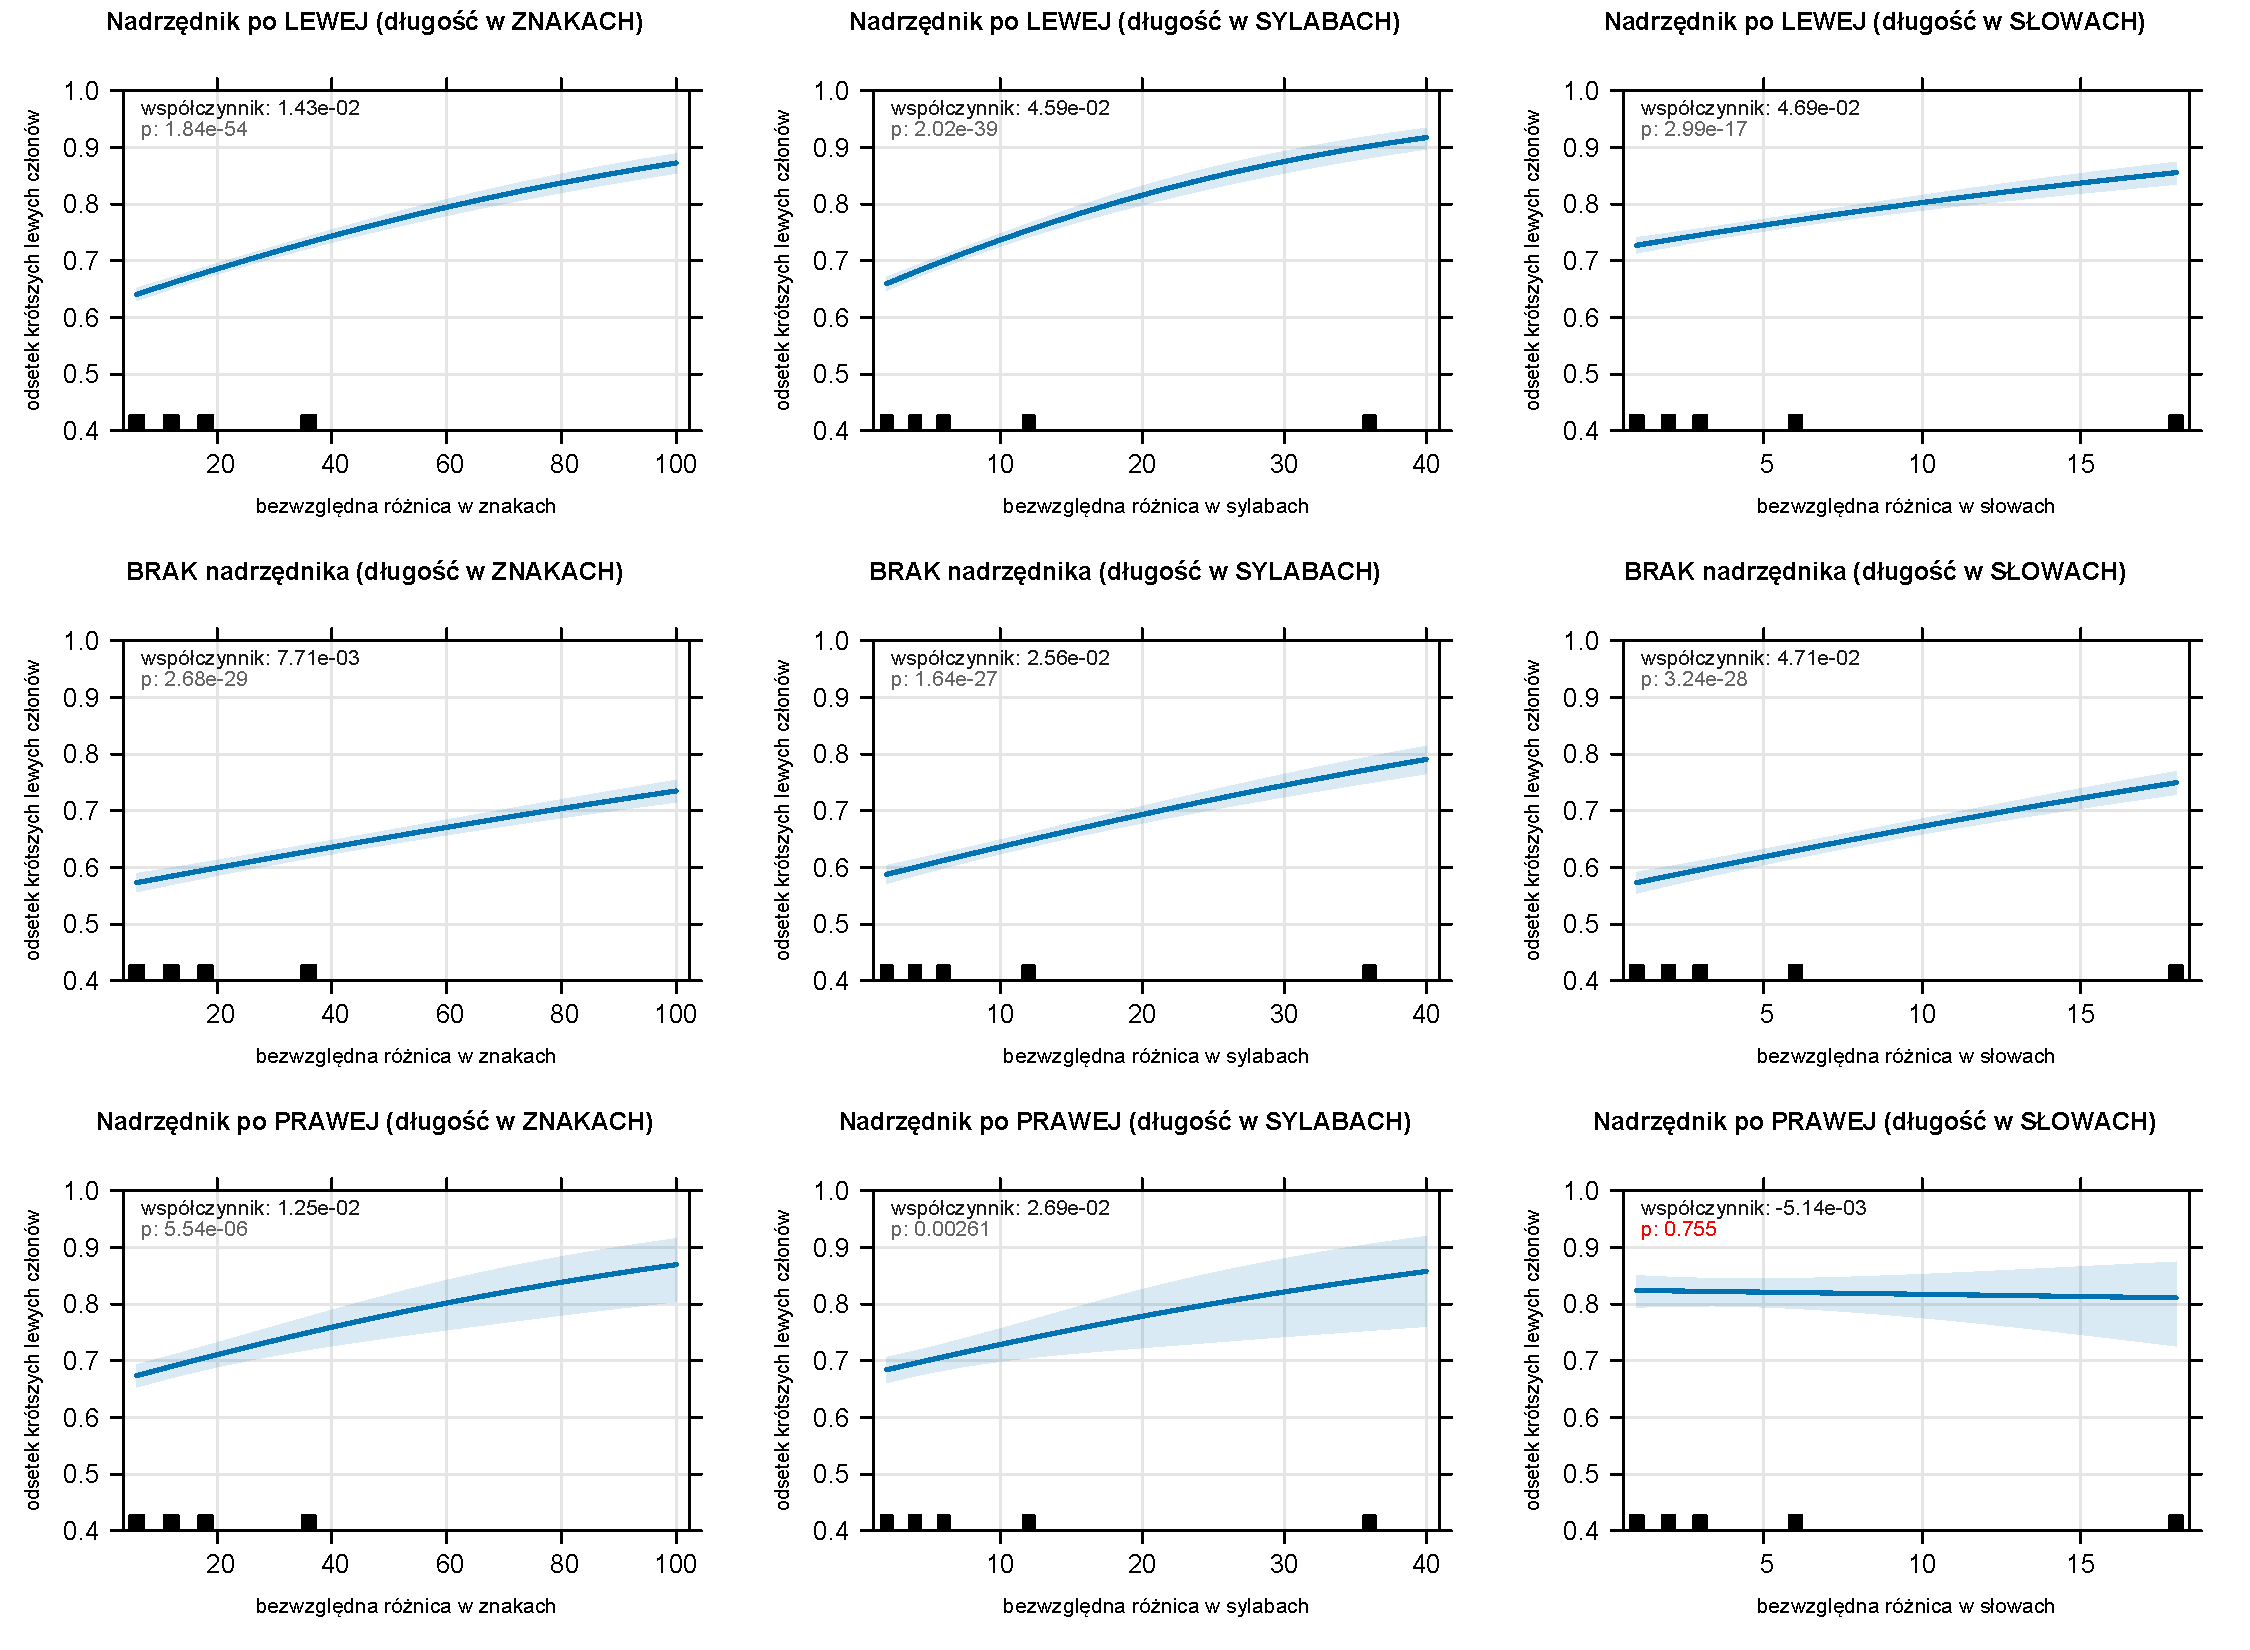
\includegraphics[scale=0.6]{English.pdf}
\caption{Różnica długości członów a występowanie krótszego członu po lewej stronie -- język \textbf{angielski} (\textbf{inicjalny, germański})}
\label{fig:angielski}
\end{sidewaysfigure}

\begin{sidewaysfigure}
\centering
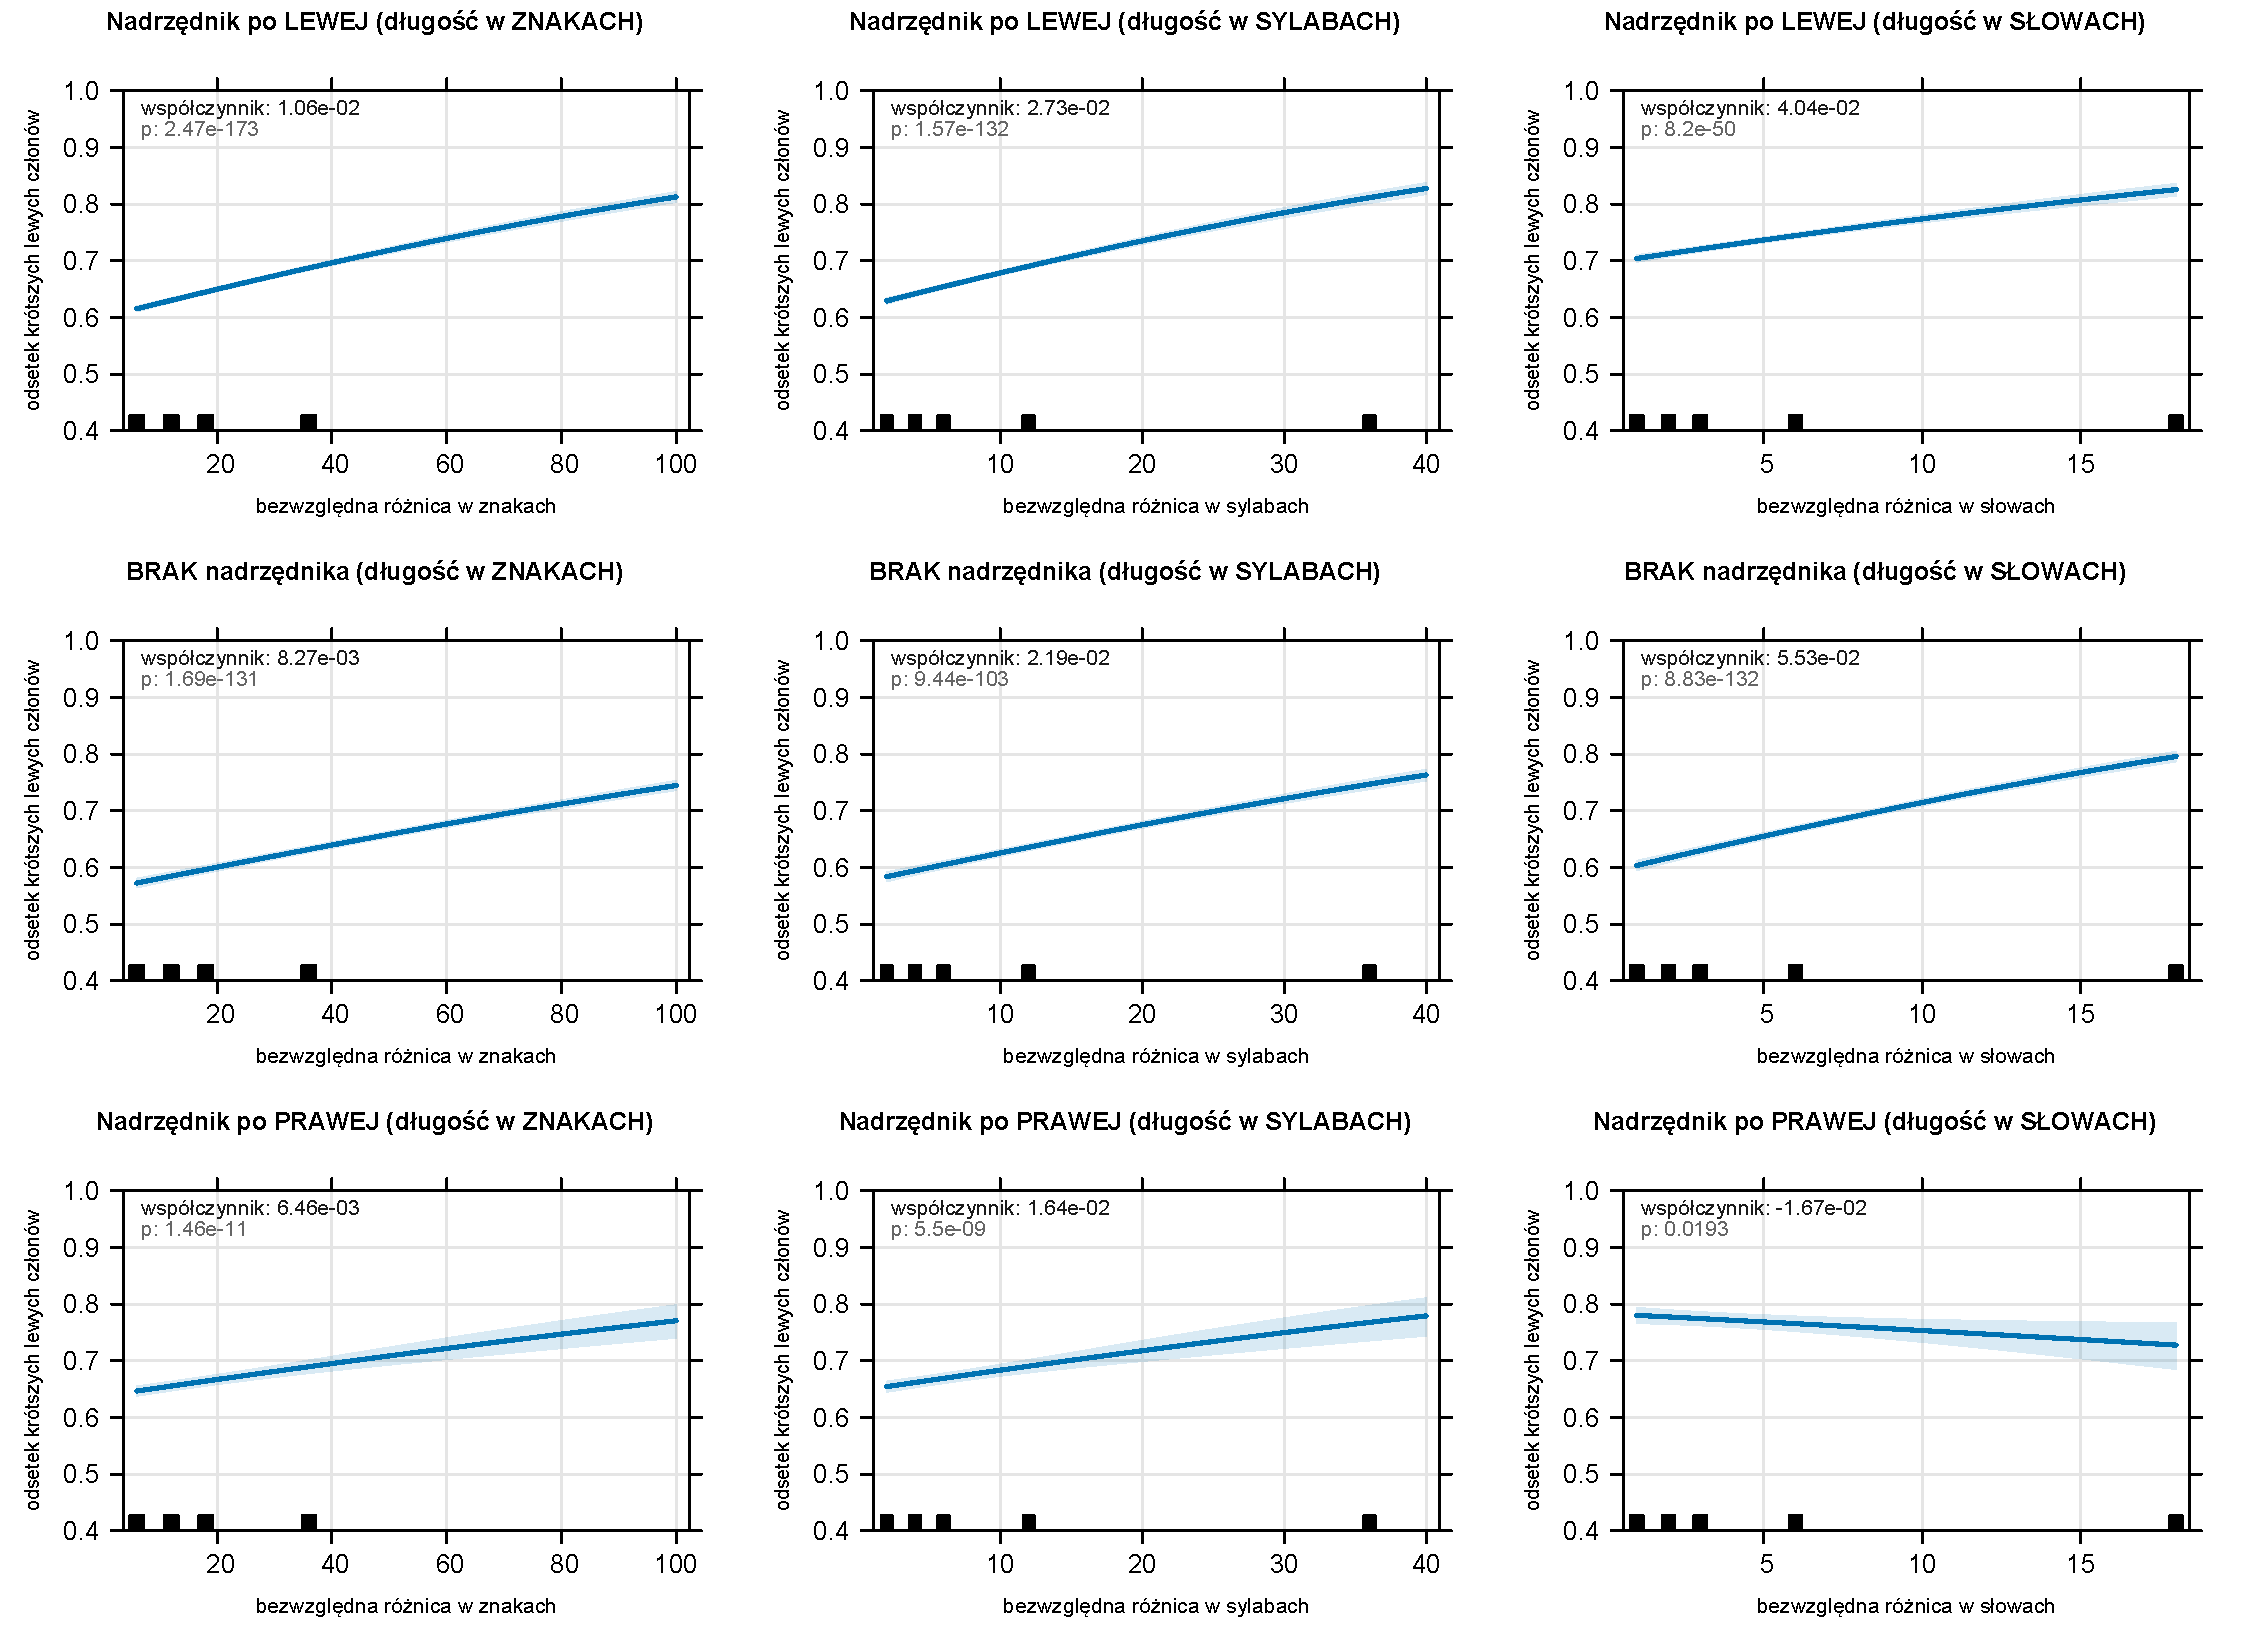
\includegraphics[scale=0.6]{Czech.pdf}
\caption{Różnica długości członów a występowanie krótszego członu po lewej stronie -- język \textbf{czeski} (\textbf{inicjalny, słowiański})}
\label{fig:czeski}
\end{sidewaysfigure}

\begin{sidewaysfigure}
\centering
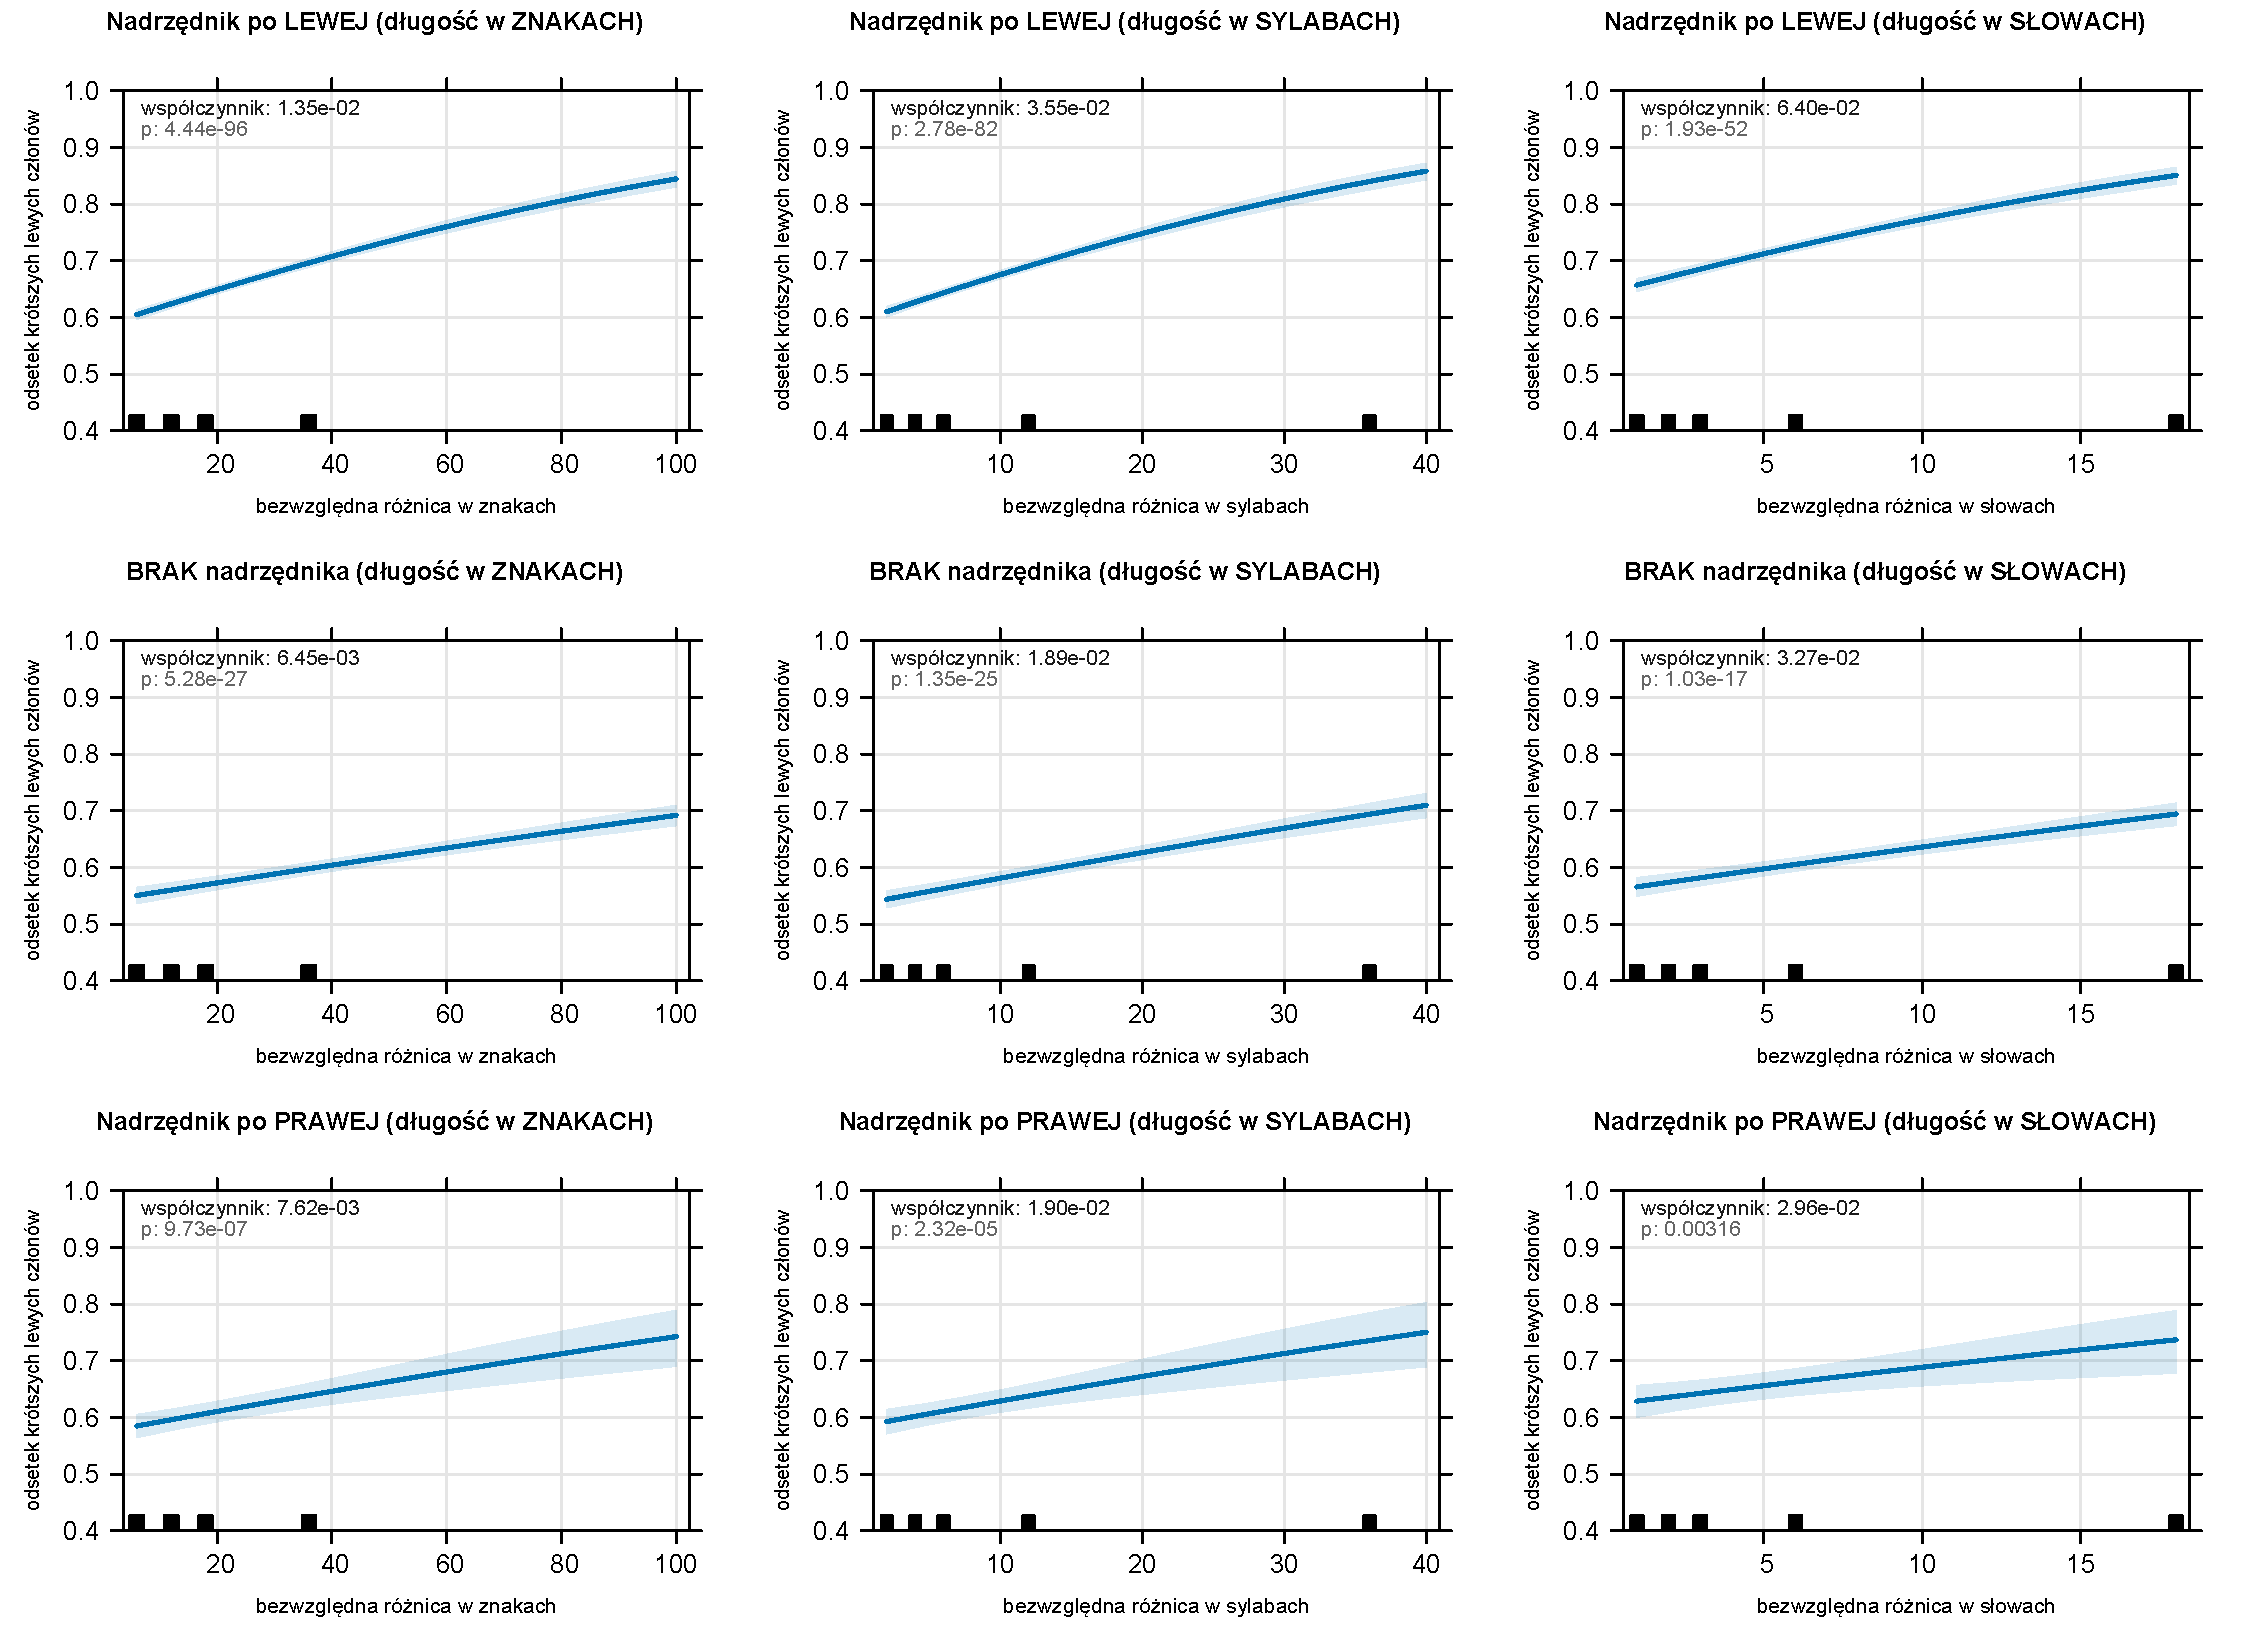
\includegraphics[scale=0.6]{Portuguese.pdf}
\caption{Różnica długości członów a występowanie krótszego członu po lewej stronie -- język \textbf{portugalski} (\textbf{inicjalny, romański})}
\label{fig:portugalski}
\end{sidewaysfigure}

\begin{sidewaysfigure}
\centering
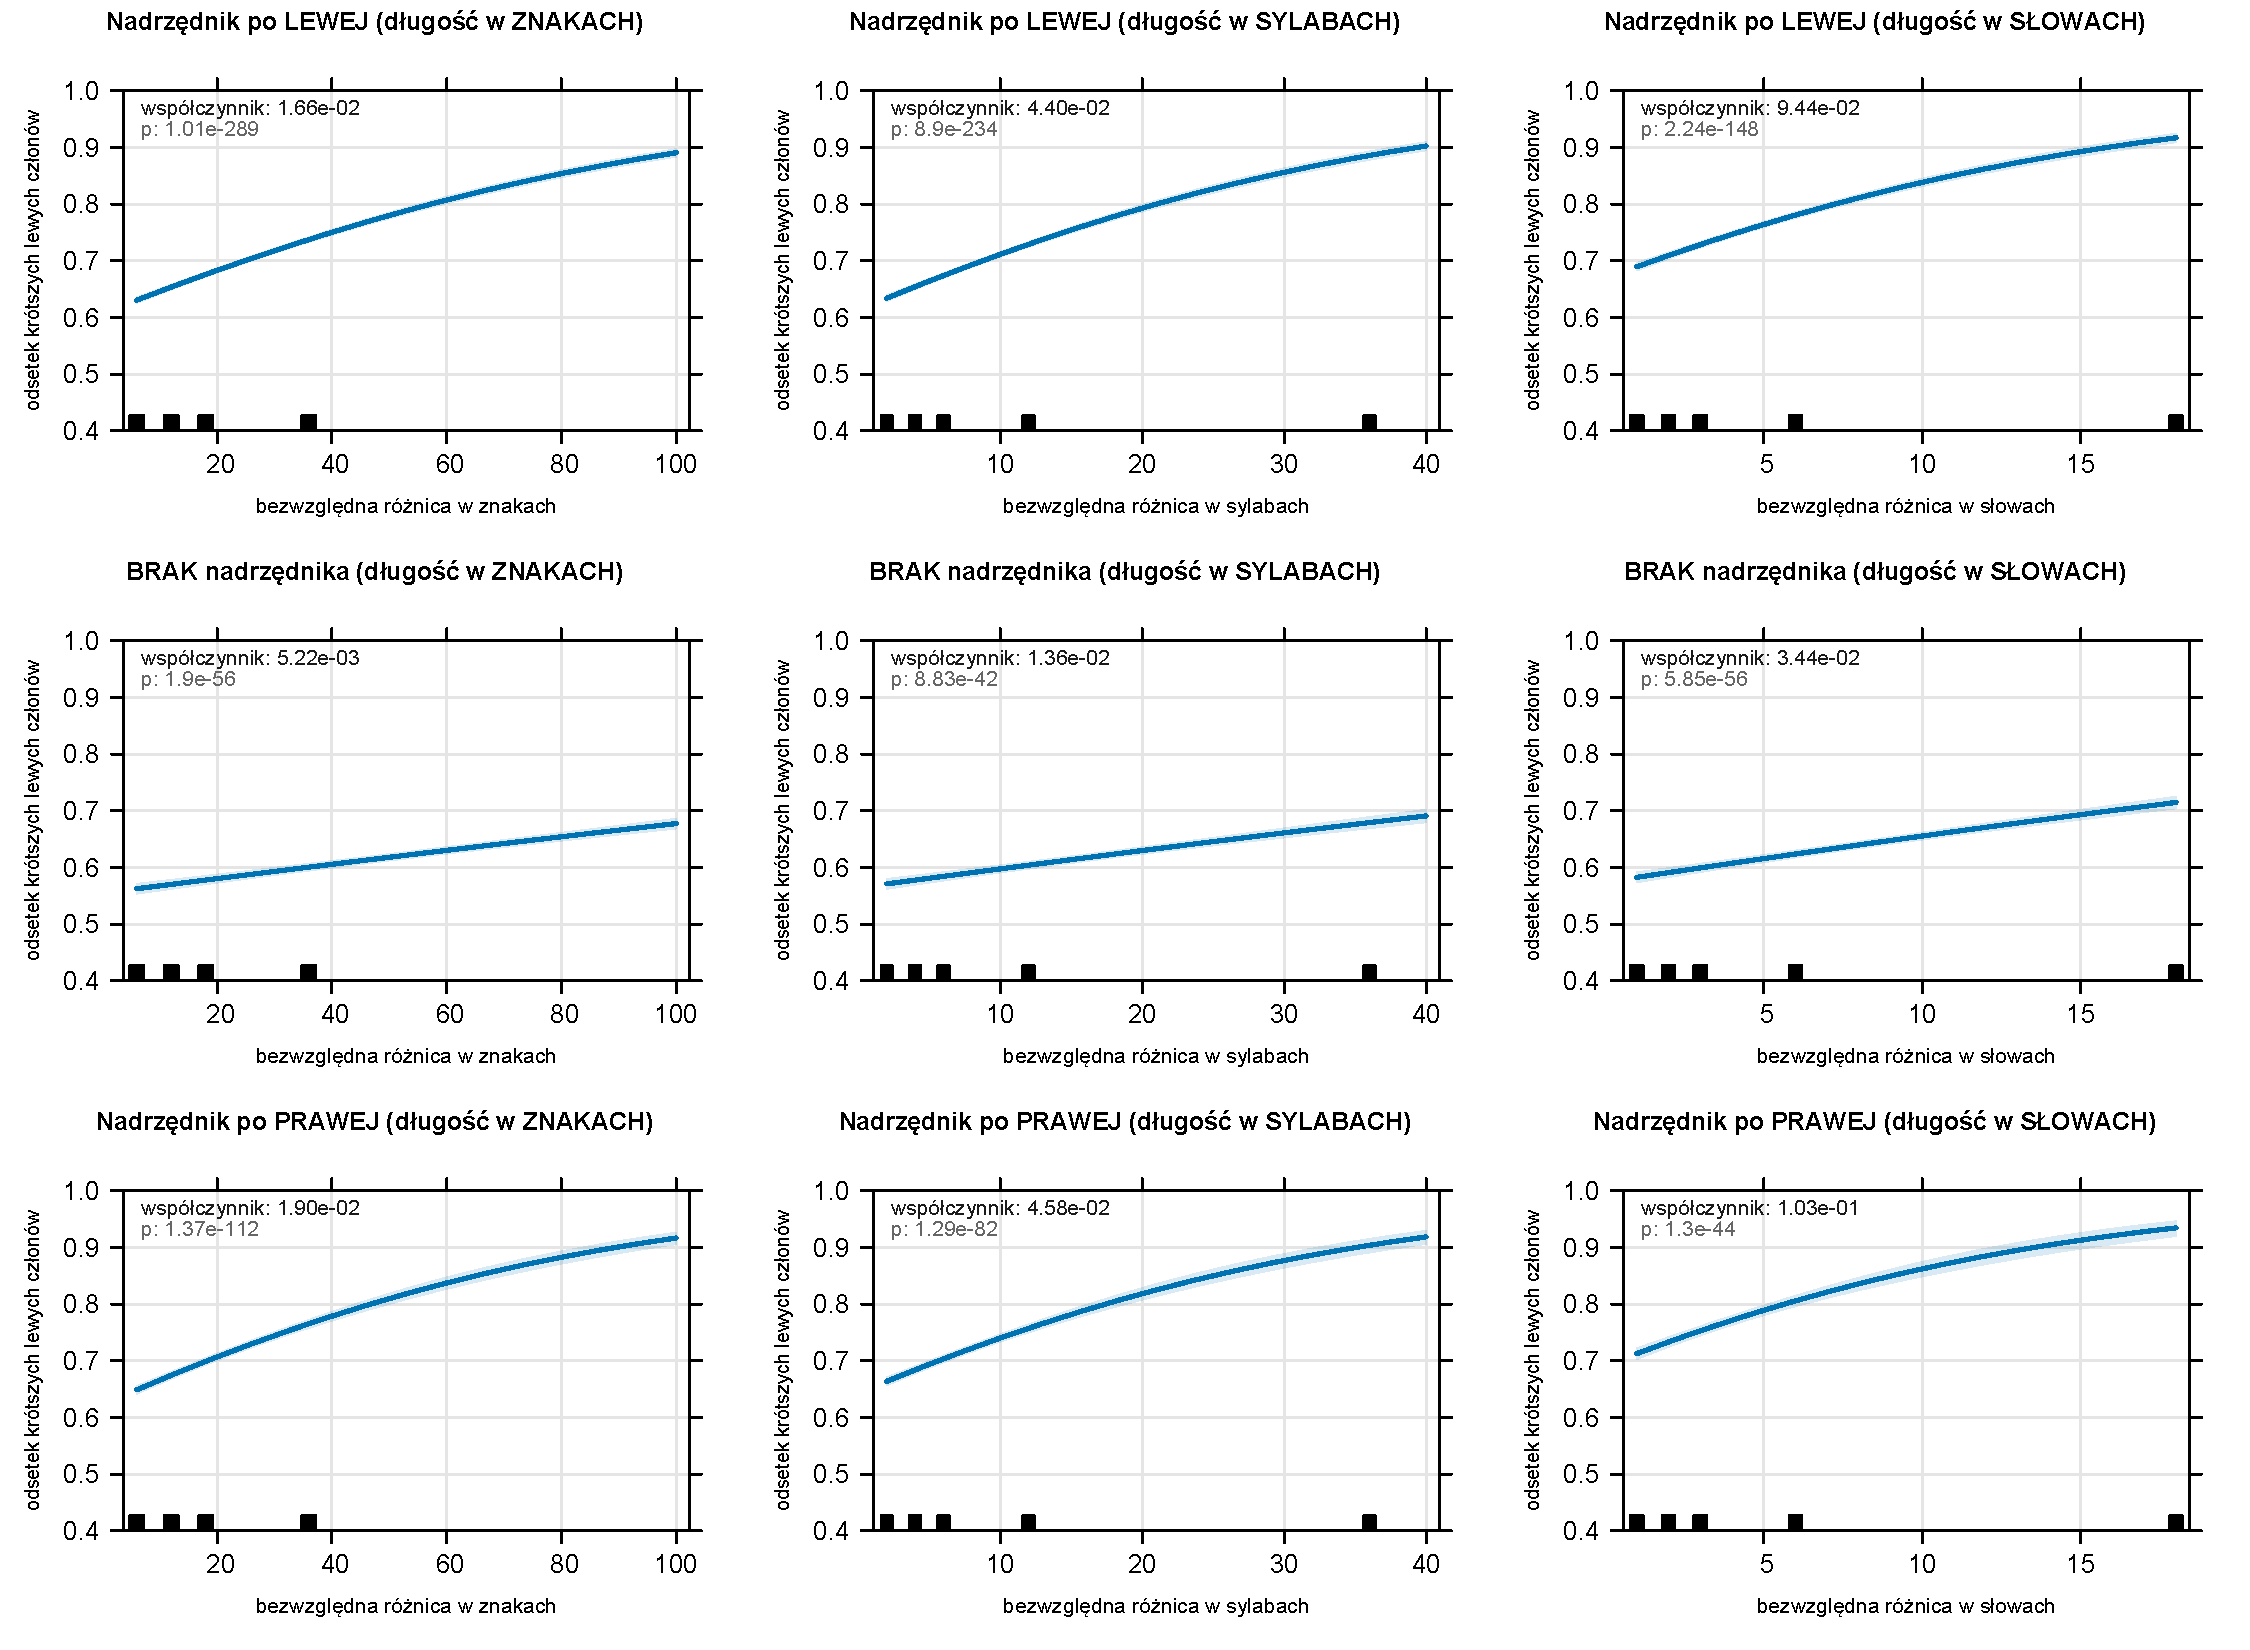
\includegraphics[scale=0.6]{German.pdf}
\caption{Różnica długości członów a występowanie krótszego członu po lewej stronie -- język \textbf{niemiecki} (\textbf{mieszany})}
\label{fig:niemiecki}
\end{sidewaysfigure}

\begin{sidewaysfigure}
\centering
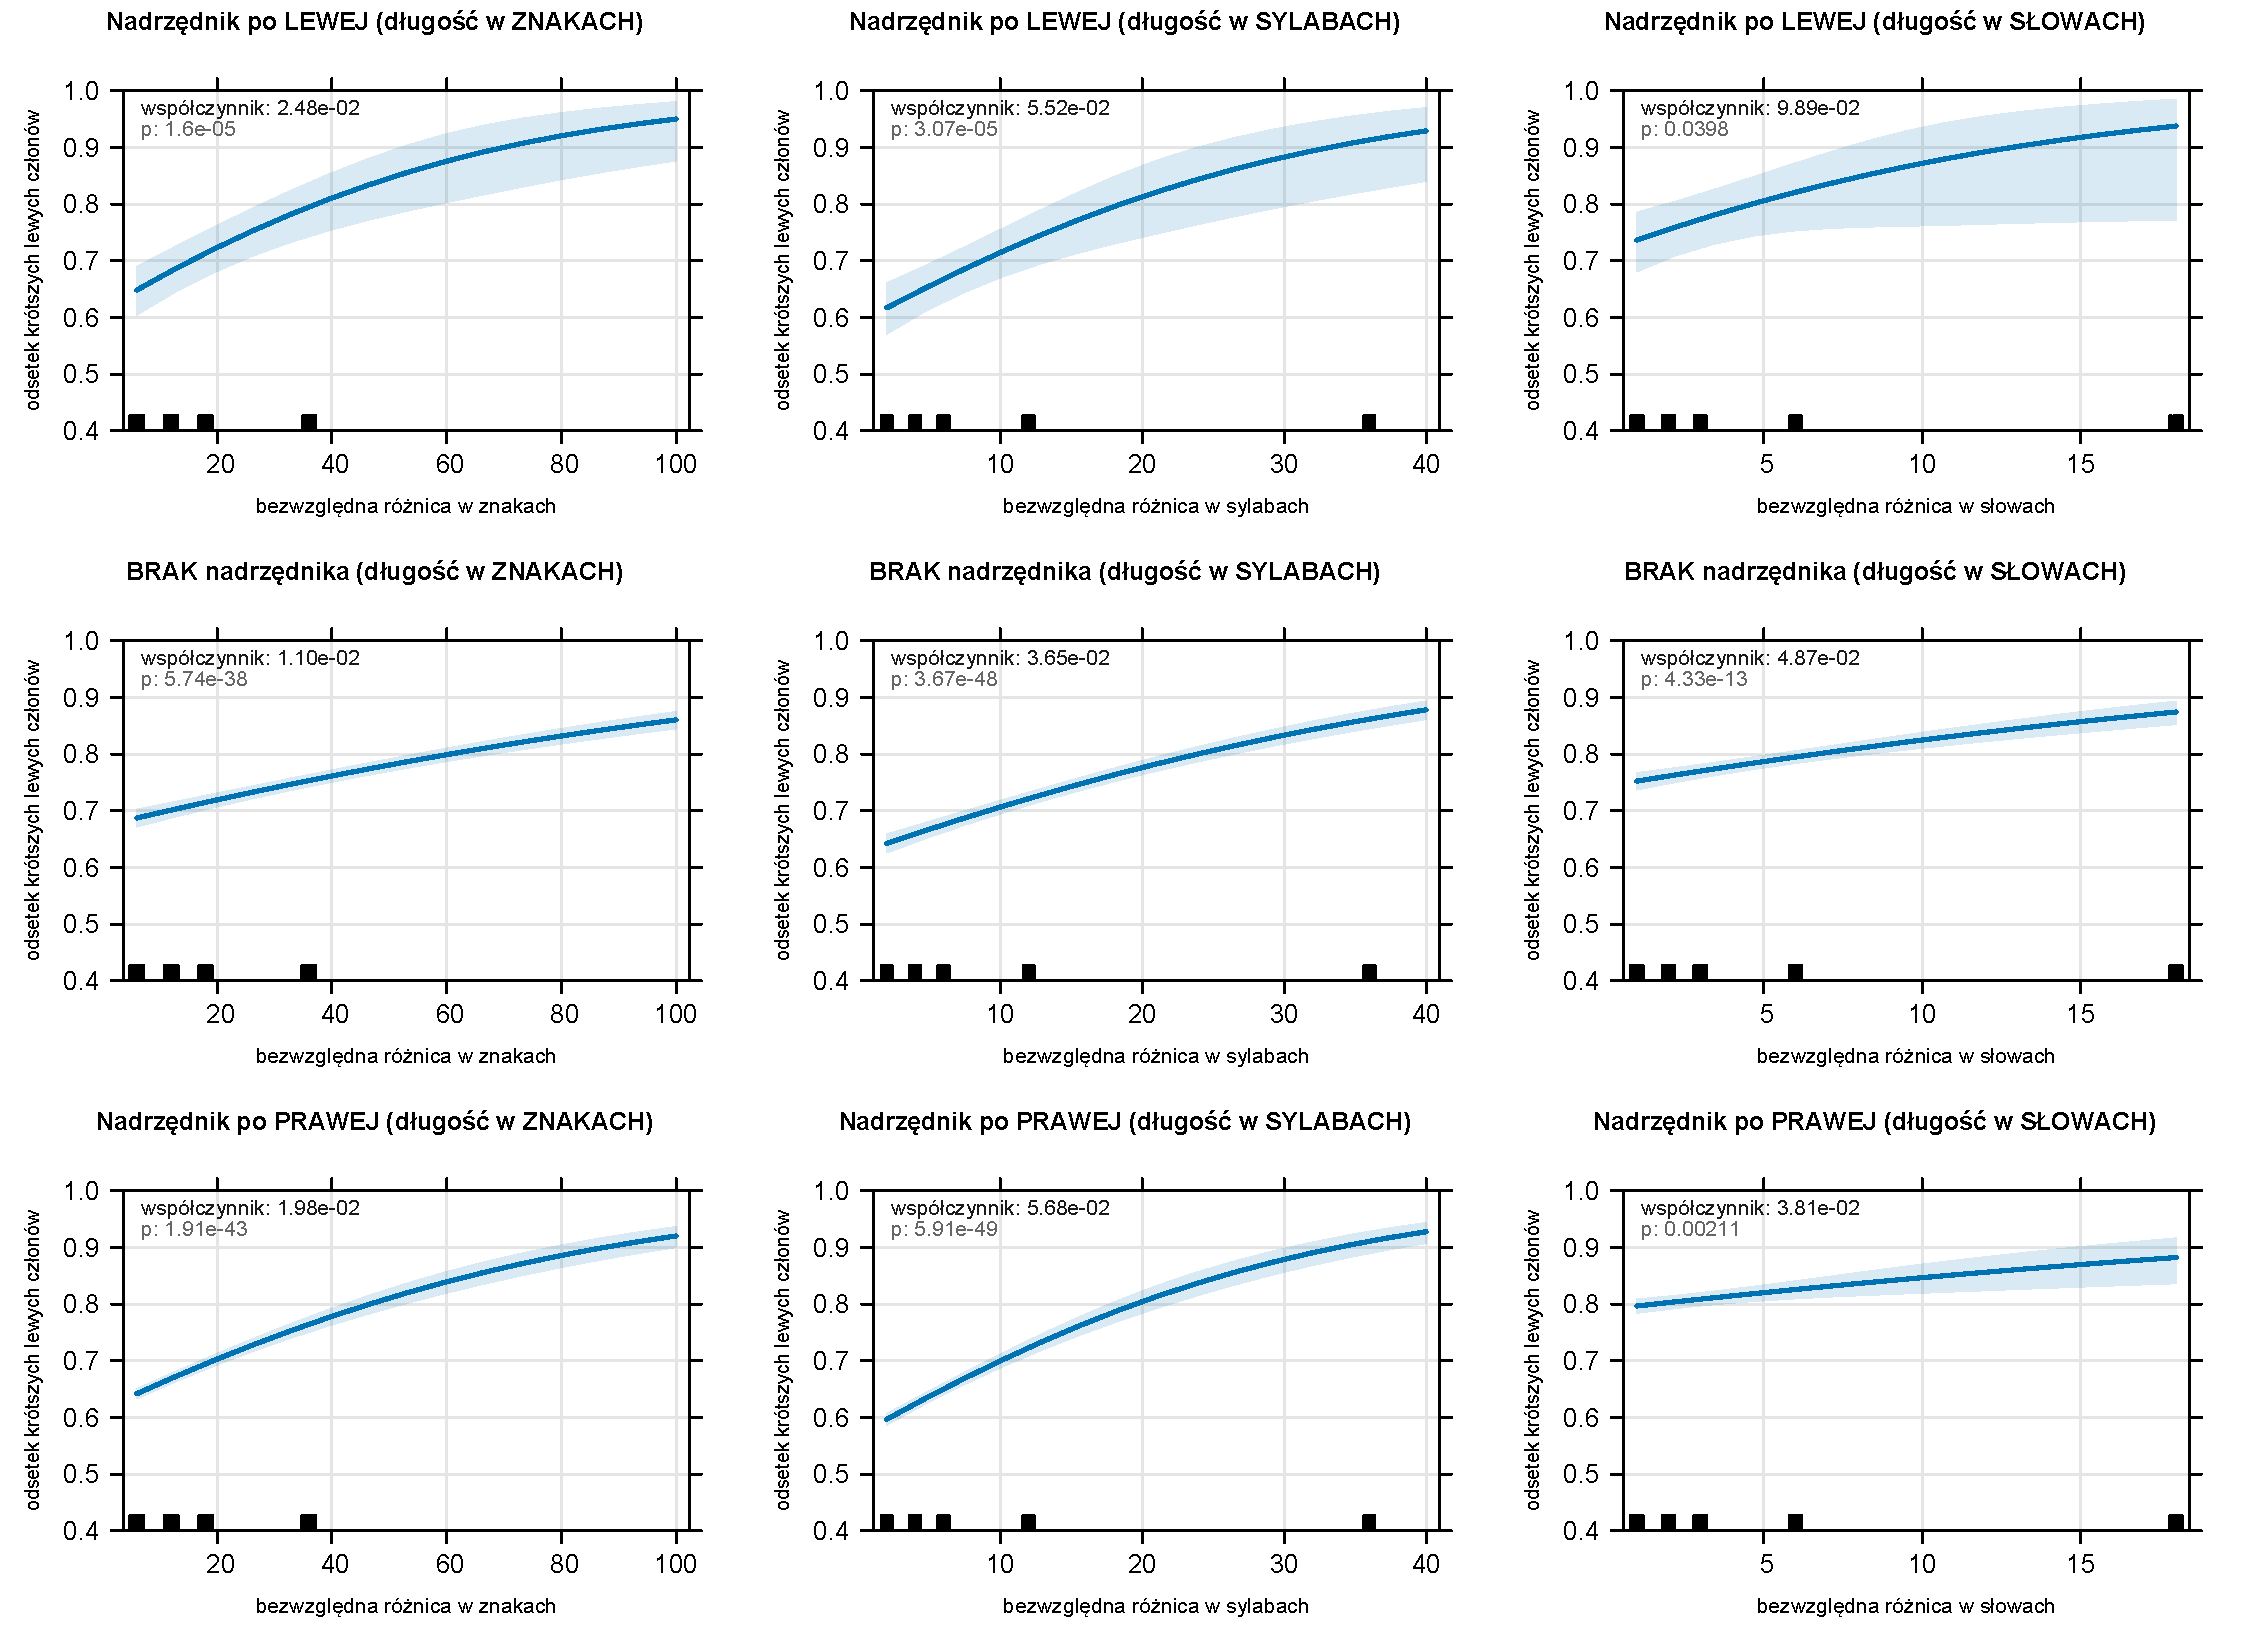
\includegraphics[scale=0.6]{Korean.pdf}
\caption{Różnica długości członów a występowanie krótszego członu po lewej stronie -- język \textbf{koreański} (\textbf{finalny})}
\label{fig:koreański}
\end{sidewaysfigure} % Metody statystyczne
%\chapter{Dyskusja wyników} \label{ch6}

\section{Replikacja poprzednich badań}

\subsection{Język angielski}

\cite{przepiorkowski2023conjunct} opisali dwie zależności dotyczące zmian tendencji do umieszczania krótszego członu koordynacji na jej początku wraz ze wzrostem różnic długości między członami koordynacji w~języku angielskim: tendencje pozytywną w koordynacjach z nadrzędnikiem po lewej stronie (L) oraz bez nadrzędnika (0) oraz (nieistotną statystycznie) tendencję negatywną w~koordynacjach z nadrzędnikiem po prawej stronie (R).

Niniejsza analiza replikuje obserwację pozytywną dotyczącą koordynacji (L) oraz~(0). W przypadku koordynacji typu (R) zależność jest pozytywna, gdy długość liczona jest w~znakach ($p<0,001$) i~sylabach ($p=0,003$).
Gdy długość członów liczona jest w słowach, tendencja jest negatywna i nieistotna statystycznie ($p=0,755$).

Te wyniki należy interpretować w kontekście efektu DLM. Polega on na minimalizacji łącznej długości relacji zależnościowych w~języku. Długość zależności może być liczona na różne sposoby. Najlepszym z nich jest najprawdopodobniej złożoność syntaktyczna frazy \citep{lohmann2014english}. Spośród stosowanych przez mnie miar (słowa, sylaby, znaki) najbliższą złożoności syntaktycznej są słowa. W~związku z~tym uznaję wyniki dotyczące długości członów w~słowach za istotniejsze od pozostałych.

Oznacza to, że~niniejsza analiza replikuje badanie \cite{przepiorkowski2023conjunct} w~zakresie opisu relacji między różnicą długości członów koordynacji a tendencją do umieszczania krótszego członu jako pierwszego w~języku angielskim.

\subsection{Języki słowiańskie}

W języku czeskim zależność dotycząca koordynacji (R) jest podobna do tej w~języku angielskim. Jest to tendencja spadkowa istotna statystycznie na poziomie $p=0,019$. Tendencje w~języku polskim oraz rosyjskim nie są istotne statystycznie. Może to oznaczać, że w~językach słowiańskich występuje ta sama zależność między pozycją nadrzędnika a zmianą odsetka koordynacji (R-L) względem (R), co w~języku angielskim. Znaczy to, że niniejsze badanie rozszerza wyniki pracy \cite{przepiorkowski2023conjunct} na język czeski oraz nie wyklucza, że omawiane tendencje występują w~pozostałych językach słowiańskich.

\subsection{Języki romańskie}

Wyniki dla analizowanych języków romańskich pokazują jednoznaczną istotną statystycznie tendencję pozytywną we wszystkich rozpatrywanych przypadkach. Oznacza to, że w~językach włoskim, hiszpańskim i~portugalskim krótszy człon koordynacji znajduje się tym częściej jako pierwszy, im krótszy jest on od ostatniego członu niezależnie od pozycji nadrzędnika. 

W przypadku języka rumuńskiego omawiana tendencja nie jest istotna statystycznie ($p=0,29$). Warto zauważyć, że język ten pomimo należenia do grupy języków romańskich jest pod silnym wpływem języków słowiańskich.

\subsection{Języki mieszane}

W przypadku języka niemieckiego widoczne są podobne tendencje, jak w~przypadku języków romańskich, zaś w~łacinie występuje taka zależność, jak w~języku angielskim i~w~językach słowiańskich. Ponieważ metodologia niniejszej pracy nie zakładała przewidywań dotyczących tendencji występujących w~tych językach, nie interpretuję tych wyników w~kontekście replikacji badania \cite{przepiorkowski2023conjunct}.

\subsection{Języki finalne}

W języku koreańskim widoczna jest ewidentna tendencja wzrostowa we~wszystkich przypadkach. Jest ona znacznie istotna statystycznie ($p<0,001$) w przypadku koordynacji pozbawionych nadrzędnika, istotna na poziomie $p=0,002$ dla koordynacji (L) oraz na poziomie $p=0,04$ dla koordynacji (R). Jest to podobna tendencja do tej zaobserwowanej w~językach romańskich i~języku niemieckim. W przypadku języka tureckiego tendencja jest wyraźnie słabsza. W przypadku koordynacji (L) nie jest ona istotna statystycznie ($p=0,29$).

\section{Przewidywania modeli struktury zależnościowej koordynacji}

\subsection{Języki inicjalne}

Jak zostało to omówione w punkcie \ref{podejścia}, istnieją cztery przyjmowane podejścia do struktury zależnościowej koordynacji:

\begin{table}[H]

\centering

\begin{tabular}{c c}

\textbf{Spójnikowe/Praskie}

&

\textbf{Wielogłowe/Londyńskie}

\\

\begin{dependency}[hide label, edge unit distance=0.5ex]

        \begin{deptext}
        $\odot$\&$\square$\&$\square$\&$\square$\&,\&$\square$\&$\square$\&$\square$\&$\boxdot$\&$\square$\&$\square$\&$\square$\\
            \end{deptext}
            \depedge{1}{9}{}
            \depedge{9}{2}{}
            \depedge{9}{6}{}
            \depedge{9}{10}{}
            \wordgroup{1}{2}{4}{c1}
            \wordgroup{1}{6}{8}{c2}
            \wordgroup{1}{10}{12}{c3}
        \end{dependency}

&

\begin{dependency}[hide label, edge unit distance=0.5ex]

        \begin{deptext}
        $\odot$\&$\square$\&$\square$\&$\square$\&,\&$\square$\&$\square$\&$\square$\&$\boxdot$\&$\square$\&$\square$\&$\square$\\
            \end{deptext}
            \depedge{1}{2}{}
            \depedge{1}{6}{}
            \depedge{1}{10}{}
            \depedge{10}{9}{}
            \wordgroup{1}{2}{4}{c1}
            \wordgroup{1}{6}{8}{c2}
            \wordgroup{1}{10}{12}{c3}
        \end{dependency}

\vspace{.5cm}
\\ 

\textbf{Bukietowe/Stanfordzkie}

&

\textbf{Łańcuchowe/Moskiewskie}

\\

\begin{dependency}[hide label, edge unit distance=0.5ex]

        \begin{deptext}
        $\odot$\&$\square$\&$\square$\&$\square$\&,\&$\square$\&$\square$\&$\square$\&$\boxdot$\&$\square$\&$\square$\&$\square$\\
            \end{deptext}
            \depedge{1}{2}{}
            \depedge{2}{6}{}
            \depedge{2}{10}{}
            \depedge{10}{9}{}
            \wordgroup{1}{2}{4}{c1}
            \wordgroup{1}{6}{8}{c2}
            \wordgroup{1}{10}{12}{c3}
        \end{dependency}

&

\begin{dependency}[hide label, edge unit distance=0.5ex]

        \begin{deptext}
        $\odot$\&$\square$\&$\square$\&$\square$\&,\&$\square$\&$\square$\&$\square$\&$\boxdot$\&$\square$\&$\square$\&$\square$\\
            \end{deptext}
            \depedge{1}{2}{}
            \depedge{2}{6}{}
            \depedge{6}{9}{}
            \depedge{9}{10}{}
            \wordgroup{1}{2}{4}{c1}
            \wordgroup{1}{6}{8}{c2}
            \wordgroup{1}{10}{12}{c3}
        \end{dependency}

\end{tabular}
\end{table}


Podejścia praskie i~londyńskie nazywane są symetrycznymi, zaś stanfordzkie i~moskiewskie -- asymetrycznymi. \cite{przepiorkowski2023conjunct} na podstawie przeprowadzonej analizy korpusowej języka angielskiego argumentują, że jedynie podejścia symetryczne (praskie i~londyńskie) mogą poprawnie opisywać strukturę zależnościową konstrukcji współrzędnie złożonej. Opierają swoje rozumowanie na predykcjach modeli dotyczących zmiany tendencji do umieszczania krótszego członu koordynacji na jej początku wraz ze~wzrostem różnicy długości członów.

Wszystkie cztery podejścia, zgodnie z faktami, przewidują tendencję pozytywną w~przypadku koordynacji (L). Dla koordynacji (0) podejścia praskie, stanfordzkie i~moskiewskie poprawnie przewidują tendencje pozytywne, zaś podejście londyńskie (wbrew faktom) przewiduje brak zależności. Kluczowa jest zależność dotycząca koordynacji (R). Podejścia symetryczne przewidują tendencję spadkową, zaś podejścia asymetryczne tendencję wzrostową.

Ponieważ w~języku angielskim omawiana tendencja dla koordynacji (R) jest negatywna, \cite{przepiorkowski2023conjunct} odrzucają podejścia asymetryczne. Bronią jednocześnie podejścia londyńskiego na podstawie argumentu o gramatykalizacji. Zgodnie z nim fakt, że koordynacje (L) występują w~języku angielskim znacznie częściej niż (R) powoduje, że umieszczanie pierwszego członu jako pierwszego mogło stać się regułą.

Wyniki przeprowadzonej przeze mnie analizy w~zakresie języka angielskiego i~języków słowiańskich nie zaprzeczają przywołanej wyżej argumentacji. Niemniej jednak wyniki dotyczące pozostałych języków inicjalnych wskazują na występowanie zupełnie innych tendencji w~językach romańskich. Istnieją przynajmniej dwa możliwe wyjaśnienia takiego zjawiska.

Zależności widoczne w~językach romańskich są zgodne z przewidywaniami modeli asymetrycznych. Istnieje więc możliwość, że języki romańskie posiadają odrębną strukturę zależnościową koordynacji niż ta występująca w~języku angielskim i~w~językach słowiańskich.

Drugie wyjaśnienie takiego stanu rzeczy jest oparte na argumencie o gramatykalizacji. Możliwe że gramatykalizacja umieszczania krótszego członu po lewej stronie koordynacji jest w~przypadku języków romańskich tak silna, że niezależnie od faktycznej struktury zależnościowej koordynacji efekt DLM nie ma większego wpływu na ustawienie członów. Innymi słowy, krótszy człon zawsze występuje częściej z lewej strony tym częściej, im większa jest różnica długości członów niezależnie od pozycji nadrzędnika.

\subsection{Języki finalne}

Tendencje zaobserwowane w~językach finalnych są znacznie trudniejsze do wyjaśnienia na podstawie efektu DLM. Jak zostało to pokazane w punkcie \ref{wszystkie-podejścia}, istnieje 16 możliwych podejść do struktury zależnościowej koordynacji:

\begin{table}[h]
\centering
\begin{tabular}{ c c c c }
(A)
\begin{dependency}[theme = simple, edge unit distance=0.5ex, baseline=-\the\dimexpr\fontdimen22\textfont2\relax]
        \begin{deptext}
        $\odot$ \& $\square$ \& $\boxdot$ \& $\square$\\
            \end{deptext}
		\depedge{1}{3}{}
		\depedge{3}{2}{}
		\depedge{3}{4}{}
        \end{dependency}
&
(B)
\begin{dependency}[theme = simple, edge unit distance=0.5ex, baseline=-\the\dimexpr\fontdimen22\textfont2\relax]
        \begin{deptext}
         $\odot$ \& $\square$ \& $\boxdot$ \& $\square$\\
	\end{deptext}
		\depedge{1}{2}{}
		\depedge{1}{4}{}
		\depedge{4}{3}{}
        \end{dependency}
& 
(C)
\begin{dependency}[theme = simple, edge unit distance=0.5ex, baseline=-\the\dimexpr\fontdimen22\textfont2\relax]
        \begin{deptext}
        $\odot$ \& $\square$ \& $\boxdot$ \& $\square$\\
            \end{deptext}
		\depedge{1}{2}{}
		\depedge{1}{4}{}
		\depedge{2}{3}{}
        \end{dependency}
& 
(D)
\begin{dependency}[theme = simple, edge unit distance=0.5ex, baseline=-\the\dimexpr\fontdimen22\textfont2\relax]
        \begin{deptext}
        $\odot$ \& $\square$ \& $\boxdot$ \& $\square$\\
            \end{deptext}
		\depedge{1}{2}{}
		\depedge{2}{3}{}
		\depedge{3}{4}{}
        \end{dependency}
\\ 
(E)
\begin{dependency}[theme = simple, edge unit distance=0.5ex, baseline=-\the\dimexpr\fontdimen22\textfont2\relax]
        \begin{deptext}
        $\odot$ \& $\square$ \& $\boxdot$ \& $\square$\\
            \end{deptext}
		\depedge{1}{4}{}
		\depedge{4}{3}{}
		\depedge{3}{2}{}
        \end{dependency}
&
(F)
\begin{dependency}[theme = simple, edge unit distance=0.5ex, baseline=-\the\dimexpr\fontdimen22\textfont2\relax]
        \begin{deptext}
        $\odot$ \& $\square$ \& $\boxdot$ \& $\square$\\
            \end{deptext}
		\depedge{1}{2}{}
		\depedge{2}{4}{}
		\depedge{4}{3}{}
        \end{dependency}
& 
(G)
\begin{dependency}[theme = simple, edge unit distance=0.5ex, baseline=-\the\dimexpr\fontdimen22\textfont2\relax]
        \begin{deptext}
        $\odot$ \& $\square$ \& $\boxdot$ \& $\square$\\
            \end{deptext}
		\depedge{1}{4}{}
		\depedge{4}{2}{}
		\depedge{4}{3}{}
        \end{dependency}
& 
(H)
\begin{dependency}[theme = simple, edge unit distance=0.5ex, baseline=-\the\dimexpr\fontdimen22\textfont2\relax]
        \begin{deptext}
        $\odot$ \& $\square$ \& $\boxdot$ \& $\square$\\
            \end{deptext}
		\depedge{1}{2}{}
		\depedge{2}{4}{}
		\depedge{2}{3}{}
        \end{dependency}
\\  
(I)
\begin{dependency}[theme = simple, edge unit distance=0.5ex, baseline=-\the\dimexpr\fontdimen22\textfont2\relax]
        \begin{deptext}
        $\odot$ \& $\square$ \& $\boxdot$ \& $\square$\\
            \end{deptext}
		\depedge{1}{4}{}
		\depedge{4}{2}{}
		\depedge{2}{3}{}
        \end{dependency}
&
(J)
\begin{dependency}[theme = simple, edge unit distance=0.5ex, baseline=-\the\dimexpr\fontdimen22\textfont2\relax]
        \begin{deptext}
        $\odot$ \& $\square$ \& $\boxdot$ \& $\square$\\
            \end{deptext}
		\depedge{1}{2}{}
		\depedge{1}{3}{}
		\depedge{1}{4}{}
        \end{dependency}
& 
(K)
\begin{dependency}[theme = simple, edge unit distance=0.5ex, baseline=-\the\dimexpr\fontdimen22\textfont2\relax]
        \begin{deptext}
        $\odot$ \& $\square$ \& $\boxdot$ \& $\square$\\
            \end{deptext}
		\depedge{1}{2}{}
		\depedge{1}{3}{}
		\depedge{3}{4}{}
        \end{dependency}
& 
(L)
\begin{dependency}[theme = simple, edge unit distance=0.5ex, baseline=-\the\dimexpr\fontdimen22\textfont2\relax]
        \begin{deptext}
        $\odot$ \& $\square$ \& $\boxdot$ \& $\square$\\
            \end{deptext}
		\depedge{1}{3}{}
		\depedge{1}{4}{}
		\depedge{3}{2}{}
        \end{dependency}
 \\
(M)
\begin{dependency}[theme = simple,  edge unit distance=0.5ex, baseline=-\the\dimexpr\fontdimen22\textfont2\relax]
        \begin{deptext}
        $\odot$ \& $\square$ \& $\boxdot$ \& $\square$\\
            \end{deptext}
		\depedge{1}{3}{}
		\depedge{1}{4}{}
		\depedge{4}{2}{}
        \end{dependency}
&
(N)
\begin{dependency}[theme = simple, edge unit distance=0.5ex, baseline=-\the\dimexpr\fontdimen22\textfont2\relax]
        \begin{deptext}
        $\odot$ \& $\square$ \& $\boxdot$ \& $\square$\\
            \end{deptext}
		\depedge{1}{3}{}
		\depedge{1}{2}{}
		\depedge{2}{4}{}
        \end{dependency}
& 
(O)
\begin{dependency}[theme = simple, edge unit distance=0.5ex, baseline=-\the\dimexpr\fontdimen22\textfont2\relax]
        \begin{deptext}
        $\odot$ \& $\square$ \& $\boxdot$ \& $\square$\\
            \end{deptext}
		\depedge{1}{3}{}
		\depedge{3}{2}{}
		\depedge{2}{4}{}
        \end{dependency}
& 
(P)
\begin{dependency}[theme = simple, edge unit distance=0.5ex, baseline=-\the\dimexpr\fontdimen22\textfont2\relax]
        \begin{deptext}
        $\odot$ \& $\square$ \& $\boxdot$ \& $\square$\\
            \end{deptext}
		\depedge{1}{3}{}
		\depedge{3}{4}{}
		\depedge{4}{2}{}
        \end{dependency}
\end{tabular}
\end{table}


Jak pokazuję w~rozdziale \ref{ch3}, żadne z nich nie przewiduje zaobserwowanej tendencji pozytywnej dla koordynacji (R). Żadne z podejść nie przewiduje też bardziej pozytywnej tendencji dla koordynacji (L) niż dla koordynacji (R). Oznacza to, że nie istnieje struktura zależnościowa koordynacji, która może tłumaczyć uzyskane wyniki. Jednocześnie niemożliwe jest, żeby koordynacja nie posiadała żadnej struktury zależnościowej. 

Uzyskanie niewyjaśnialnych wyników może oznaczać, że~metodologia niniejszej pracy jest niewystarczająca w~celu poprawnego i~jednoznacznego opisu struktury zależnościowej koordynacji.

\section{Wyjaśnienia wyników}

\subsection{Gramatykalizacja krótszego prawego członu} \label{gramatykalizacja}

Z~Tabel \ref{tab:czeski+angielski} i~\ref{tab:niemiecki+koreański} wynika, że we wszystkich badanych językach, niezależnie od pozycji nadrzędnika krótszy człon koordynacji znajduje się częściej na jej początku. Może to oznaczać, że umieszczanie najkrótszego jako pierwszego uległo gramatykalizacji.

W przypadku języków inicjalnych, przyczyny tej gramatykalizacji są proste w~wyjaśnieniu. Każde z~czterech omawianych podejść zakłada, że w~przypadku  koordynacji z~nadrzędnikiem po lewej stronie wzrost różnicy długości członów przekłada się na częstsze umieszczanie krótszego członu na początku koordynacji. Ponieważ w~językach inicjalnych koordynacje z~nadrzędnikiem po lewej stronie są znacznie częstsze od pozostałych (a w~wielu przypadkach stanowią ponad połowę konstrukcji współrzędnie złożonych), umieszczanie krótszego członu po lewej stronie stało się w~tych językach regułą. 

Niemniej jednak zastosowanie analogicznego rozumowania nie wyjaśnia tendencji uzyskanych w językach finalnych. Żadne z~analizowanych podejść nie zakłada częstszego umieszczania krótszego członu na początku koordynacji wraz ze wzrostem różnicy długości członów niezależnie od pozycji nadrzędnika. Oznacza to, że umieszczanie krótszego członu po lewej stronie nie może wynikać z tego, że koordynacje (R) są częstsze w~językach finalnych.

Jeśli w~językach finalnych umieszczanie krótszego członu po lewej stronie koordynacji uległo gramatykalizacji, musi wynikać to z~innych przyczyn, niż ze~struktury składniowej koordynacji. 

\subsection{Monotoniczność tendencji}

Dependency Length Minimisation jest zjawiskiem polegającym na możliwym skracaniu relacji zależnościowych występujących w~zdaniach. Jego wpływ na ustawianie kolejności członów koordynacji można traktować jako funkcję bezwzględnej różnicy długości członów w~prawdopodobieństwo wystąpienia krótszego członu po lewej stronie. Nie wiadomo nic na temat działania tej funkcji, oprócz tego, że jest ona monotoniczna.

Niemniej jednak istnieje możliwość, że pomimo, że efekt DLM ma charakter funkcji monotonicznej, tendencja do zmiany proporcji umieszczania krótszego członu po lewej stronie koordynacji wraz ze zmianą różnicy długości członów nie jest monotoniczna. 

\cite{przepiorkowski2024argument} przeprowadzili replikację analizy z~pracy \cite{przepiorkowski2023conjunct} na większym korpusie języka angielskiego. Przeanalizowali 11 502 053 koordynacji. Dla porównania, \cite{przepiorkowski2023conjunct} zbadali 21 825 konstrukcji współrzędnie złożonych, a w~niniejszej pracy przeanalizowano 21 013 koordynacji języka angielskiego. Wyniki dotyczące koordynacji (L) i~(0) potwierdziły tendencje zaobserwowane z pracy \cite{przepiorkowski2023conjunct}. 

W przypadku koordynacji (R) \cite{przepiorkowski2024argument} zaobserwowali niemonotoniczną zależność między zmianą odsetka występowania krótszych członów na początku koordynacji a różnicą długości członów. Dla niewielkiej różnicy długości (nie przekraczającej 4 słów lub 30 znaków) dla koordynacji (R) zaobserwowano tendencję rosnącą, zaś dla większych różnic tendencję malejącą. 

Możliwe, że w~przypadku badanych przeze mnie języków istnieją podobne zależności. Jeśli tak jest, taki kształt relacji  może wynikać z interakcji między dwiema przeciwnymi tendencjami. W koordynacjach (R) efekt DLM składa się na tendencję spadkową, zaś inne przyczyny na tendencje wzrostową. W przypadku konstrukcji z małą różnicą długości członów efekt DLM jest słaby i~nie jest widoczny. Dopiero~gdy różnica długości przekracza pewien próg (na przykład czterech słów) efekt DLM staje się silniejszy niż pozostałe tendencje wzrostowe.

Niestety, weryfikacja powyższych spekulacji za pomocą korpusów zależnościowych UD jest niemożliwa. W~analizowanych danych znajduje się zbyt mało koordynacji (R) o dużej różnicy długości członów, żeby można było na ich podstawie utworzyć istotny statystycznie model.

\subsection{Przyczyny tendencji wzrostowych}

\cite{przepiorkowski2023conjunct} twierdzą, że tendencje wzrostowe dla koordynacji (0) mogą wynikać z~gramatykalizacji umieszczania krótszego członu po lewej stronie. Jak pokazuję w~puncie \ref{gramatykalizacja}, wyjaśnienie to może opisywać jedynie wyniki uzyskane dla języków inicjalnych. Gramatykalizacja ta nie może zachodzić w~językach inicjalnych lub może zachodzić w~inny sposób, niż twierdzą \cite{przepiorkowski2023conjunct}.

W niniejszym punkcie przedstawiam argument mogący stanowić wyjaśnienie występowania różnych tendencji dotyczących koordynacji (R) w~badanych przeze mnie językach.

W rozdziale \ref{ch2} opisuję różne przyczyny, dla których w~języku występuje naturalna tendencja do umieszczania krótszego członu koordynacji po lewej stronie. Należą do nich czynniki pragmatyczne, psycholingwistyczne (argument o częstym używaniu krótszych słów) oraz  wynikające z prozodii (argument o rozłożeniu sylab akcentowanych). 

\cite{wright2005ladies} wskazują, że czynniki wynikające z prozodii mają szczególnie mocny wpływ na koordynacje krótkie, tj. o członach jedno- i~dwusylabowych. W przypadku takich koordynacji różnica długości członów jest zwykle niewielka, więc efekt DLM może być pomijalny.

Jak wskazują \cite{mcdonald1993word}, koordynacje o krótkich członach są konstruowane tak, żeby akcentowane sylaby tworzyły rytm. Pokazują to poniższe przykłady:

\begin{exe}
\ex \label{jan+maria-obiad} {
\metrics{   _   u |   _   u   |  _   u | _  u  }
        {[[Jan] i | [Ma-ria]] |  \textit{zje}-\textit{dli} | o-biad.}
        }
        
\ex \label{maria+jan-obiad} {
\metrics{   _   u  u   _      _   u _   u  }
        {[[Ma-ria] i [Jan]] \textit{zje}-\textit{dli} o-biad.}
        }
        
\ex \label{obiad-jan+maria} {
\metrics{_   u  |   _   u |    _   u |   _   u   }
        {O-biad | \textit{zje}-\textit{dli} | [[Jan] i | [Ma-ria]].}
        }

\ex \label{obiad-maria+jan} {
\metrics{_   u    _   u    _   u  u   _    }
        {O-biad \textit{zje}-\textit{dli} [[Ma-ria] i [Jan]].}
        }
\end{exe}
        
W przykładach \eqref{jan+maria-obiad} i~\eqref{maria+jan-obiad} nadrzędnik koordynacji \textit{zjedli} znajduje się po lewej stronie, zaś w~przykładach \eqref{obiad-jan+maria} i~\eqref{obiad-maria+jan} po prawej stronie. Rytm oparty o stopy metryczne powstaje tylko w~zdaniach, w~których krótszy człon \textit{Jan} występuje jako pierwszy, tj. w~\eqref{jan+maria-obiad} i~\eqref{obiad-jan+maria}. W tych przykładach rozkład sylab akcentowanych jest niezależny od pozycji nadrzędnika. Zgodnie z argumentacją przedstawioną w~pracy \cite{mcdonald1993word} to właśnie zdania \eqref{jan+maria-obiad} i~\eqref{obiad-jan+maria} mają większą szansę na pojawienie się w~języku naturalnym niż zdania \eqref{maria+jan-obiad} i~\eqref{obiad-maria+jan}\footnote{
Warto zauważyć, że przykład zdań \eqref{jan+maria-obiad}--\eqref{obiad-maria+jan} stanowi szczególny przypadek, w którym jeden z członów koordynacji posiada jedną, zaś drugi dwie sylaby. W przypadku koordynacji, w której człony miałyby odpowiednio dwie i trzy sylaby, tendencje byłyby odwrotne. Podane przykłady nie mają na celu wykazania, że prozodia ma większy wpływ na ustawienie członów koordynacji niż efekt DLM ani udowodnienia częstości występowania koordynacji z członami jedno- i dwusylabowymi. Zdania \eqref{jan+maria-obiad}--\eqref{obiad-maria+jan} mają na celu jedynie pokazać, że mogą istnieć sytuacje, w których rozkład sylab akcentowanych ma większy wpływ na ustawienie członów koordynacji niż efekt DLM. Do określenia, jak częste jest to zjawisko i jaka jest jego faktyczna interakcja z efektem DLM, należałoby przeprowadzić osobne badanie.
}.

To samo rozumowanie nie ma zastosowania w~przypadku koordynacji z większą różnicą długości członów.

  \begin{exe}
\ex \label{jan+maria-obiad-długie} {
\metrics{   u  _  u   _  u   _   u   u  _   u     _   u    _  u u   _   u   _   u    _    u _   u  }
        {[[Wy-so-ki bru-net Jan] i [ko-bie-ta w~śre-dnim wie-ku i-mie-niem Ma-ria]] \textit{zje}-\textit{dli} o-biad.}
        }
        
\ex \label{maria+jan-obiad-długie} {
\metrics{   u  _   u     _   u    _  u u   _   u   _  u   u   u  _  u   _  u   _      _   u  _  u  }
        {[[Ko-bie-ta w~śre-dnim wie-ku i-mie-niem Ma-ria] i [wy-so-ki bru-net Jan]] \textit{zje}-\textit{dli} o-biad.}
        }
        
\ex \label{obiad-jan+maria-długie} {
\metrics{_   u    _   u    u  _  u   _  u   _   u    u  _   u     _   u   _  u u   _   u  _   u    }
        {O-biad \textit{zje}-\textit{dli} [[wy-so-ki bru-net Jan] i [ko-bie-ta w~śre-dnim wie-ku i-mie-niem Ma-ria]].}
        }

\ex \label{obiad-maria+jan-długie} {
\metrics{_   u    _   u    u  _  u   _  u   _   u   u  _   u     _   u    _  u _   u   _  u   u    }
        {O-biad \textit{zje}-\textit{dli} [[ko-bie-ta w~śre-dnim wie-ku i-mie-niem Ma-ria] i [wy-so-ki bru-net Jan]].}
        }
\end{exe}      

Dodatkowe podrzędniki głów członów \textit{Jan} oraz \textit{Maria} w~przykładach \eqref{jan+maria-obiad-długie}--\eqref{obiad-maria+jan-długie} zaburzają rytm we wszystkich czterech przypadkach. Niezależnie od pozycji krótszego członu osiągnięcie pożądanej sekwencji naprzemiennie występujących sylab krótkich i~długich jest niemożliwy\footnote{\setstretch{1.5}
Rytm zawsze występuje w~części zdania -- np. fraza \metrics{u _ | u _ | u _}{Wy-so | ki bru | net Jan} dzieli się na trzy stopy jambiczne. Kluczowe jest ustawienie sylab na krawędziach członu: we~fragmencie \metrics{_ u u u _ u}{Ma-ria i wy-so-ki} nie występuje rytm.}.
Powoduje to, że omawiany efekt prozodyczny nie ma w~tych przykładach zastosowania. W takiej sytuacji większe znaczenie dla ustawienia kolejności członów może mieć efekt DLM. Jeśli prawidłowe są podejścia symetryczne (jak argumentują \citealt{przepiorkowski2023conjunct}), to zdanie \eqref{maria+jan-obiad-długie} ma większą szansę pojawić się w~języku, niż zdanie \eqref{jan+maria-obiad-długie}, zaś zdanie \eqref{obiad-jan+maria-długie} ma większą szansę niż \eqref{obiad-maria+jan-długie}.

Kluczową różnicą między zdaniami \eqref{jan+maria-obiad}--\eqref{obiad-maria+jan} i~\eqref{jan+maria-obiad-długie}--\eqref{obiad-maria+jan-długie} jest długość członów występujących w~nich koordynacji. Możliwe, że w~przypadku krótszych członów rytm występuje częściej niż w~przypadku dłuższych, ponieważ każdy dodatkowy podrzędnik głowy członu ma szansę na jego zaburzenie. W takiej sytuacji w~koordynacjach z krótszymi członami większy wpływ ma efekt ustawienia sylab akcentowanych, zaś w~przypadku zdań z dłuższymi koordynacjami efekt DLM.

Koordynacje z dużą różnicą długości członów (przekraczającą kilka słów) są możliwe tylko wtedy, kiedy jeden z członów jest długi. Możliwe,  że~w~przypadku koordynacji z większą różnicą długości członów jest więcej koordynacji z długimi członami, niż w~przypadku koordynacji z małą różnicą długości członów. Jeśli to prawda, zgodnie z omówioną powyżej hipotezą efekt DLM ma większy wpływ od efektu wynikającego z prozodii tylko w~przypadku koordynacji z różnicą długości członów przekraczającą kilka słów. W takim przypadku interakcja tych dwóch efektów jest jednym z~możliwych wyjaśnień wyników uzyskanych w~badaniu \citep{przepiorkowski2024argument}

To zjawisko może również tłumaczyć zaobserwowane w~niniejszej pracy różnice między językami. Typowe rozkłady sylab akcentowanych różnią się w~zależności od języka. Ponadto, mogą być one zależne w~większym stopniu od przynależności do danej rodziny językowej niż związane z inicjalnością lub finalnością języka. Jeśli w~językach romańskich i~języku koreańskim rytm zdania ma większy wpływ na ułożenie kolejności słów w~zdaniu i~nie jest tak łatwo zaburzany jak w~języku angielskim i~językach słowiańskich, może to być wyjaśnieniem otrzymanych wyników.

Weryfikacja postawionej w~niniejszym punkcie hipotezy nie jest możliwa na podstawie metod i~danych użytych w~niniejszej pracy. W~następnym rozdziale~\ref{ch7} omawiam przyczyny tego faktu oraz propozycje badań mogących sprawdzić opisaną przeze mnie hipotezę.
 % Dyskusja wyników
%\chapter{Zakończenie} \label{ch7}

\section{Ograniczenia}

\subsection{Korpusy zależnościowe UD}

Jednym z głównych ograniczeń niniejszej pracy jest korzystanie wyłącznie z~korpusów zależnościowych Universal Dependencies. Dzięki standardowemu opisowi relacji składniowej korpusy UD umożliwiają miarodajną analizę wielu różnych języków naraz. Jednak ze względu na wymuszanie przez UD konkretnego sposobu opisu struktur, korpusy mogą tracić na jakości.

\paragraph{Ograniczenia dla języków finalnych}
\cite{choi2011statistical} oraz \cite{kanayama2018coordinate} wskazują, że tworzenie korpusów zależnościowych zgodnie z~narzucanym przez UD podejściem stanfordzkim tworzą drzewa niezgodne z~teorią lingwistyczną. Z~tego powodu z~japońskich korpusów Universal Dependencies zostały usunięte wszystkie koordynacje, a w~korpusach koreańskich występują równolegle dwa różne standardy opisu struktur.

Powoduje to, że analiza koordynacji w korpusach japońskich jest niemożliwa, zaś w~przypadku korpusów koreańskich może być w~znacznym stopniu niemiarodajna.

\paragraph{Nieprawidłowy opis głów fraz}
Standard Universal Dependencies nie jest wyłącznie standardem składniowym; przy ustalaniu relacji zależnościowych stosuje również kryteria semantyczne. Oznacza to, że według wytycznych tego standardu głową członu nie jest faktyczna, składniowa głowa członu, lecz temat lub najważniejszy semantycznie token w~obrębie frazy. 

\begin{exe} 
\ex
\begin{dependency}[baseline=-\the\dimexpr\fontdimen22\textfont2\relax]
\begin{deptext}[column sep=1em]
Był \& ordynatorem \& w~\& szpitalu \& .  \\ 
\end{deptext}
\depedge{2}{1}{cop}
\deproot{2}{root}
\depedge{4}{3}{case}
\depedge{2}{4}{nmod}
\depedge{2}{5}{punct}
\end{dependency}
\label{UD-złe}
\end{exe}

W przykładzie \eqref{UD-złe} głową frazy \textit{w szpitalu} jest \textit{szpitalu}, zaś głową całego zdania (czyli korzeniem zdania) \textit{ordynatorem}. Zgodnie z teorią lingwistyczną głową frazy przyimkowej \textit{w szpitalu} powinien być przyimek \textit{w}, zaś korzeniem zdania z orzeczeniem imiennym -- łącznik \textit{Był} \citep{hoeksema1992head}. Traktowanie rzeczowników jako głów fraz przyimkowych i orzeczników jako korzeni zdań jest znamienne dla drzew UD. Efektem tych rozwiązań jest w~szczególności ,,przesuwanie'' głowy członu na jej koniec w~językach inicjalnych.

Niemniej jednak efekty tych rozwiązań nie powinny być na tyle powszechne, żeby mieć znaczący wpływ na wynik mojej analizy. Powtórzona poniżej tabela \ref{tab:pozycja-głowy} pokazuje względną pozycję głów członów koordynacji w~badanych językach. Gdyby w~korpusach UD faktycznie istniała częsta tendencja do nieprawidłowego oznaczania późniejszych elementów fraz jako ich głowy, średnia pozycja głowy w~językach inicjalnych byłaby większa niż 0,5. Wobec tego należy uznać znakowanie UD za~zasadniczo poprawne.

\begin{table}[H]
\centering
\begin{tabular}{lrrrrrrrr}
  \toprule
Język & \multicolumn{4}{c}{lewy człon} & \multicolumn{4}{c}{prawy człon}\\
 & \multicolumn{1}{c}{N} & \multicolumn{1}{c}{średnia} & \multicolumn{1}{c}{t} & \multicolumn{1}{c}{p} & \multicolumn{1}{c}{N} & \multicolumn{1}{c}{średnia} & \multicolumn{1}{c}{t} & \multicolumn{1}{c}{p} \\ 
  \midrule
  \multicolumn{9}{c}{\textbf{Języki inicjalne}} \\
  \midrule
  angielski 	& 12326 	& \textbf{0,36} & $-$37 & 1.74e$-$288 & 15155 & \textbf{0,40} & $-$31 & 1.99e$-$199 \\
  czeski 	& 51416 	& \textbf{0,34} & $-$88 & 0 		& 62872 & \textbf{0,39} & $-$70 & 0 \\ 
  hiszpański	& 19685 & \textbf{0,30} & $-$74 & 0 		& 22137 & \textbf{0,31} & $-$80 & 0 \\ 
  islandzki 	& 31929 	& \textbf{0,18} & $-$196 & 0 		& 36967 & \textbf{0,18} & $-$225 & 0 \\ 
  polski 	& 9976 	& \textbf{0,23} & $-$74 & 0 		& 12049 & \textbf{0,33} & $-$50 & 0 \\ 
  portugalski & 19732 & \textbf{0,30} & $-$71 & 0 		& 22349 & \textbf{0,30} & $-$84 & 0 \\ 
  rosyjski 	& 36608 	& \textbf{0,38} & $-$56 & 0 		& 46050 & \textbf{0,41} & $-$47 & 0 \\ 
  rumuński 	& 27224 	& \textbf{0,37} & $-$53 & 0 		& 31024 & \textbf{0,37} & $-$60 & 0 \\ 
  włoski 	& 17728 	& \textbf{0,43} & $-$22 & 1,2e$-$107	& 20330 & \textbf{0,37} & $-$49 & 0 \\
  \midrule
  \multicolumn{9}{c}{\textbf{Języki mieszane}} \\
  \midrule
  łaciński 	& 19766 & \textbf{0,36}	& $-$47 & 0 		& 25755 & \textbf{0,48} & $-$5,8 & 7,98e$-$09 \\
  niemiecki & 51068 	& \textbf{0,53}	& 17 & 9,27e$-$62	& 64616 & \textbf{0,52} & 14 & 2,61e$-$46 \\ 
  \midrule
  \multicolumn{9}{c}{\textbf{Języki finalne}} \\
  \midrule
  koreański	& 6801 & \textbf{0,78} & 59 & 0 			& 12951 & \textbf{0,65} & 47 & 0 \\ 
  turecki 	& 7994 & \textbf{0,64} & 28 & 7,97e$-$167	& 12763 & \textbf{0,69} & 55 & 0 \\
  \bottomrule
\end{tabular}
\caption{Względna pozycja głów członów koordynacji}
\label{tab:pozycja-głowy}
\end{table}



\subsection{Dependency Length Minimisation}

\paragraph{Założenie o monotoniczności tendencji}

Badając wpływ DLM na kolejność ustawienia członów koordynacji, zakładam, że jest on wyrażony jako monotoniczna funkcja. Z tego powodu, obliczając tendencję, korzystam z dwumianowej regresji logistycznej.

% pomijam możliwości jego interakcji z innymi czynnikami (m.in. pragmatycznymi, psycholingwistycznymi i prozodycznymi).

Dokładniejsze zbadanie właściwości efektu DLM może pozwolić na stworzenie dokładniejszych modeli, które są w~stanie estymować proporcje ustawiania członów lepiej, niż przez samo określenie, że są one opisywane przez rosnącą, malejącą lub stałą funkcję. 

\paragraph{Metoda określania złożoności}

\cite{lohmann2014english} stwierdza, że najlepszym sposobem na określenie długości relacji jest złożoność syntaktyczna rozumiana jako liczba węzłów w~relacjach składnikowych łączących słowa w~frazy. Ponieważ korzystam z korpusów zależnościowych, w~analizie nie mogę obliczyć złożoności syntaktycznej. Estymacja złożoności składniowej za pomocą liczby słów nie jest idealnym rozwiązaniem i może wpłynąć na wyniki badania.

Jest to poważne ograniczenie badania, tym bardziej, że~w~wielu badanych przeze mnie językach wyniki dotyczące słów są istotnie inne, niż wyniki korzystające z innych miar długości.

\subsection{Ograniczenia metodologiczne}

W przeprowadzonym przeze mnie badaniu analizuję koordynacje wyciągnięte automatycznie na podstawie algorytmu opartego o heurystyki. Każda z heurystyk została opracowana na podstawie wielu kompromisów i założeń oraz ze świadomością, że nie zawsze będą one działać poprawnie. Ponadto, większość heurystyk została przypisana językom bez znajomości języków, na zasadzie analogii z językiem angielskim, polskim i tureckim.

Ewaluacja losowo wyciągniętych koordynacji wykazała, że \textit{większość z nich} została wyciągnięta poprawnie. Niemniej jednak sam algorytm liczenia długości członów nie został poddany ewaluacji.

\section{Przyszłe badania}

\subsection{Surface Syntactic Universal Dependencies (SUD)}

Surface Syntactic Universal Dependencies\footnote{
\url{https://surfacesyntacticud.github.io/}
} to projekt mający na celu stworzenie alternatywnego dla UD standardu opisu relacji zależnościowych. Jest on z założenia bardziej wierny powierzchniowym relacjom składniowym, zaś na jego wytyczne nie mają wpływ argumenty semantyczne. Dzięki temu korpusy SUD są bardziej wiarygodne, jeśli chodzi o opis relacji zależnościowych i unikają problemów obecnych w~zwykłych korpusach UD.

Istnieje możliwość, że przeprowadzenie analogicznego badania na korpusach SUD pozwoliłoby uzyskać bardziej wiarygodne wyniki.

\subsection{Analiza koordynacji różnych długości}

\cite{przepiorkowski2024argument} pokazują, że omawiane tendencje dotyczące koordynacji w~języku angielskim mogą być niemonotoniczne. Z~ich badania wynika, że proste modele statystyczne, takie jak regresja logistyczna, mogą nie wystarczyć w~analizie tych zależności.

W rozdziale \ref{ch6} przedstawiam hipotezę, zgodnie z którą uwzględnienie w~analizie tylko koordynacji o dłuższych członach może pozwolić uzyskać bardziej wiarygodne wyniki. Hipoteza ta jest zgodna z wynikami uzyskanymi w~pracy \cite{przepiorkowski2024argument}. 

Niestety, konstrukcje współrzędnie złożone dłuższych członach występują w~języku bardzo rzadko. w~przypadku analizowanych przeze mnie danych uwzględnienie w~analizie wyłącznie koordynacji, których oba człony składają się z co najmniej czterech tokenów nie pozwala na stworzenie istotnych statystycznie modeli logistycznych.

Oznacza to, że korpusy UD są zbyt małe, żeby można było przeprowadzić na nich takie badanie. Analiza koordynacji różnych długości powinna zostać przeprowadzona na korpusach zawierających miliony zdań. % Konkluzje

\appendix

%\chapter{Wyniki poprzednich badań} \label{dod:PW23}

\graphicspath{{results}}
\begin{sidewaysfigure}
\centering
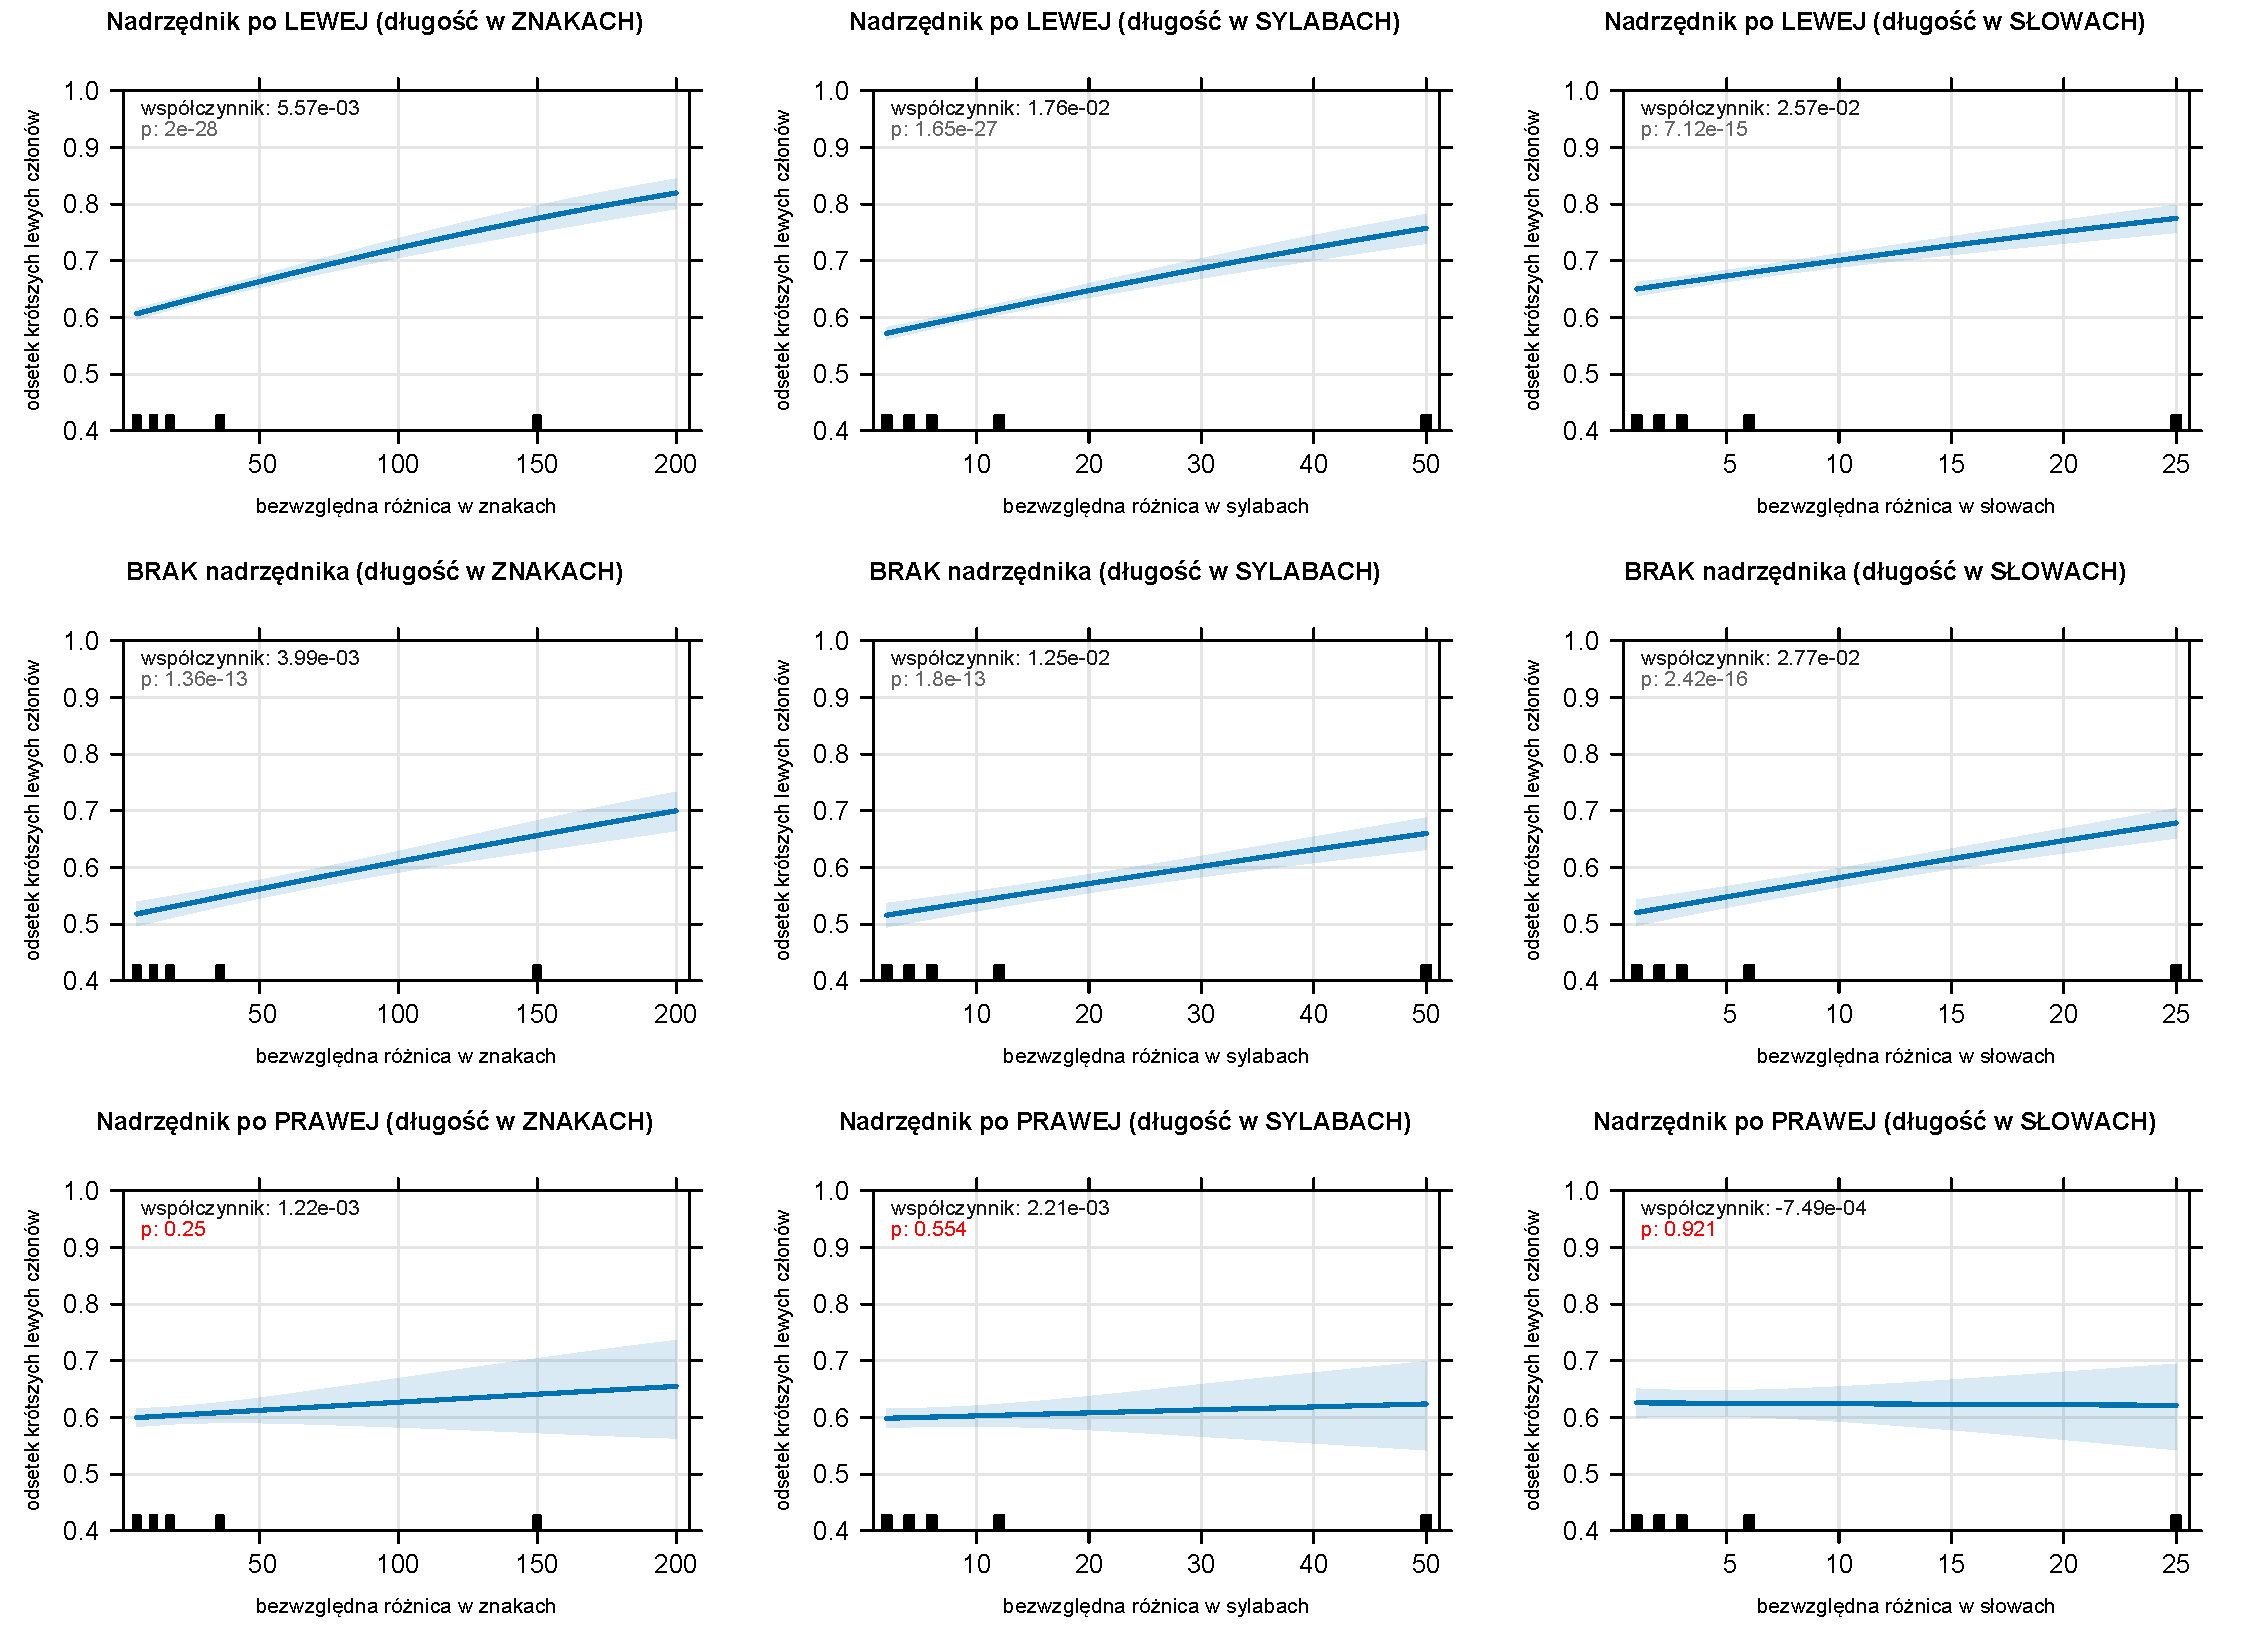
\includegraphics[scale=0.6]{PW23.pdf}
\caption{Różnica długości członów a występowanie krótszego członu po lewej stronie w języku \textbf{angielskim} --
wyniki uzyskane w~pracy \cite{przepiorkowski2023conjunct}}
\label{fig:PW23}
\end{sidewaysfigure} % Wyniki z PW23
%\chapter{Długość członów koordynacji} \label{dod:tabele}

\section{Języki inicjalne}

\begin{table}[H]
\centering
\resizebox{\linewidth}{!}{
% latex table generated in R 4,3,1 by xtable 1,8-4 package
% Sun Jun  2 11:59:07 2024
\begingroup\setlength{\tabcolsep}{4pt}
\scalebox{0.8}{
\begin{tabular}{lrrrrrr}
  \toprule
  & \multicolumn{2}{c}{mediana} & \multicolumn{2}{c}{średnia}  \\
 & \multicolumn{1}{c}{lewy} & \multicolumn{1}{c}{\hspace*{-1ex}prawy\hspace*{-1ex}} & \multicolumn{1}{c}{lewy} & \multicolumn{1}{c}{prawy} & \multicolumn{1}{c}{V} & \multicolumn{1}{c}{$p$} \\
 \midrule
 \multicolumn{7}{c}{\textbf{Język angielski}} \\
 \midrule
 \multicolumn{7}{c}{Wszystkie koordynacje (N = 21~013)} \\
  \midrule
znaki & 13 & 20 & 22,79 & 32,69 & 5,3e+07 &   0 \\ 
  sylaby & 4 & 5 & 6,00 & 8,51 & 4e+07 &   0 \\ 
  słowa & 2 & 4 & 4,19 & 5,96 & 2,3e+07 &   0 \\ 
   \midrule
 \multicolumn{7}{c}{Brak nadrzędnika (N = 6~829)} \\
 \midrule
znaki & 30 & 40 & 37,41 & 50,99 & 6,9e+06 & 7,4e-154 \\ 
  sylaby & 8 & 10 & 9,61 & 13,00 & 6e+06 & 5,7e-148 \\ 
  słowa & 6 & 8 & 7,13 & 9,65 & 5,1e+06 & 3,6e-159 \\ 
   \midrule
 \multicolumn{7}{c}{Nadrzędnik po lewej (N = 11~171)} \\
 \midrule
znaki & 10 & 16 & 17,28 & 26,49 & 1,3e+07 &   0 \\ 
  sylaby & 3 & 4 & 4,64 & 6,99 & 9,5e+06 &   0 \\ 
  słowa & 2 & 3 & 3,05 & 4,66 & 4,4e+06 &   0 \\ 
   \midrule
 \multicolumn{7}{c}{Nadrzędnik po prawej (N = 2~972)} \\
 \midrule
znaki & 7 & 9 & 10,10 & 13,90 & 8,1e+05 & 6,5e-99 \\ 
  sylaby & 2 & 2 & 2,88 & 3,88 & 4,9e+05 & 5,2e-75 \\ 
  słowa & 1 & 1 & 1,74 & 2,34 & 8e+04 & 1,8e-68 \\ 
   \bottomrule
\end{tabular}
}
\endgroup

\quad
% latex table generated in R 4.3.1 by xtable 1.8-4 package
% Sun Jun  2 11:59:00 2024
\begingroup\setlength{\tabcolsep}{4pt}
\scalebox{0.8}{
\begin{tabular}{lrrrrrr}
  \toprule
  & \multicolumn{2}{c}{mediana} & \multicolumn{2}{c}{średnia}  \\
 & \multicolumn{1}{c}{lewy} & \multicolumn{1}{c}{\hspace*{-1ex}prawy\hspace*{-1ex}} & \multicolumn{1}{c}{lewy} & \multicolumn{1}{c}{prawy} & \multicolumn{1}{c}{V} & \multicolumn{1}{c}{$p$} \\
 \midrule
 \multicolumn{7}{c}{\textbf{Język czeski}} \\
 \midrule
 \multicolumn{7}{c}{Wszystkie koordynacje (N = 90,566)} \\
  \midrule
znaki & 13 & 21 & 24.44 & 34.64 & 1e+09 &   0 \\ 
  sylaby & 5 & 8 & 8.93 & 12.43 & 8.7e+08 &   0 \\ 
  słowa & 2 & 3 & 3.70 & 5.31 & 3.8e+08 &   0 \\ 
   \midrule
 \multicolumn{7}{c}{Brak nadrzędnika (N = 26,688)} \\
 \midrule
znaki & 31 & 45 & 39.54 & 57.18 & 9.9e+07 &   0 \\ 
  sylaby & 11 & 16 & 14.16 & 20.14 & 9.3e+07 &   0 \\ 
  słowa & 5 & 7 & 6.13 & 9.08 & 7.1e+07 &   0 \\ 
   \midrule
 \multicolumn{7}{c}{Nadrzędnik po lewej (N = 49,341)} \\
 \midrule
znaki & 10 & 16 & 19.59 & 27.69 & 2.8e+08 &   0 \\ 
  sylaby & 4 & 6 & 7.28 & 10.10 & 2.4e+08 &   0 \\ 
  słowa & 1 & 2 & 2.93 & 4.14 & 8.7e+07 &   0 \\ 
   \midrule
 \multicolumn{7}{c}{Nadrzędnik po prawej (N = 14,279)} \\
 \midrule
znaki & 8 & 10 & 12.83 & 16.28 & 2.2e+07 &   0 \\ 
  sylaby & 3 & 4 & 4.81 & 6.02 & 1.6e+07 & 3.3e-291 \\ 
  słowa & 1 & 1 & 1.82 & 2.29 & 2.2e+06 & 5.1e-202 \\ 
   \bottomrule
\end{tabular}
}
\endgroup

}
\label{tab:cz+en}
\end{table}

\begin{table}[H]
\centering
\resizebox{\linewidth}{!}{
% latex table generated in R 4.3.1 by xtable 1.8-4 package
% Sun Jun  2 11:59:50 2024
\begingroup\setlength{\tabcolsep}{4pt}
\scalebox{0.8}{
\begin{tabular}{lrrrrrr}
  \toprule
  & \multicolumn{2}{c}{mediana} & \multicolumn{2}{c}{średnia}  \\
 & \multicolumn{1}{c}{lewy} & \multicolumn{1}{c}{\hspace*{-1ex}prawy\hspace*{-1ex}} & \multicolumn{1}{c}{lewy} & \multicolumn{1}{c}{prawy} & \multicolumn{1}{c}{V} & \multicolumn{1}{c}{$p$} \\
 \midrule
 \multicolumn{7}{c}{\textbf{Język hiszpański}} \\
 \midrule
 \multicolumn{7}{c}{Wszystkie koordynacje (N = 28~666)} \\
  \midrule
znaki & 18 & 26 & 30,70 & 43,79 & 1,1e+08 &   0 \\ 
  sylaby & 6 & 9 & 10,84 & 15,08 & 9,6e+07 &   0 \\ 
  słowa & 3 & 5 & 5,20 & 7,50 & 5,1e+07 &   0 \\ 
   \midrule
 \multicolumn{7}{c}{Brak nadrzędnika (N = 6~300)} \\
 \midrule
znaki & 45 & 65 & 55,91 & 79,19 & 5,7e+06 & 2e-169 \\ 
  sylaby & 16 & 22 & 19,59 & 27,08 & 5,5e+06 & 1,3e-154 \\ 
  słowa & 8 & 11 & 9,64 & 13,77 & 4,6e+06 & 5,5e-176 \\ 
   \midrule
 \multicolumn{7}{c}{Nadrzędnik po lewej (N = 19~557)} \\
 \midrule
znaki & 14 & 20 & 23,83 & 34,71 & 4,9e+07 &   0 \\ 
  sylaby & 5 & 7 & 8,46 & 12,00 & 4,2e+07 &   0 \\ 
  słowa & 2 & 3 & 3,98 & 5,88 & 1,8e+07 &   0 \\ 
   \midrule
 \multicolumn{7}{c}{Nadrzędnik po prawej (N = 2~751)} \\
 \midrule
znaki & 11 & 14 & 21,88 & 26,91 & 1e+06 & 2,6e-34 \\ 
  sylaby & 4 & 5 & 7,74 & 9,38 & 8,6e+05 & 1,8e-29 \\ 
  słowa & 2 & 2 & 3,69 & 4,59 & 3,6e+05 & 1,9e-29 \\ 
   \bottomrule
\end{tabular}
}
\endgroup

\quad
% latex table generated in R 4,3,1 by xtable 1,8-4 package
% Sun Jun  2 11:59:19 2024
\begingroup\setlength{\tabcolsep}{4pt}
\scalebox{0.8}{
\begin{tabular}{lrrrrrr}
  \toprule
  & \multicolumn{2}{c}{mediana} & \multicolumn{2}{c}{średnia}  \\
 & \multicolumn{1}{c}{lewy} & \multicolumn{1}{c}{\hspace*{-1ex}prawy\hspace*{-1ex}} & \multicolumn{1}{c}{lewy} & \multicolumn{1}{c}{prawy} & \multicolumn{1}{c}{V} & \multicolumn{1}{c}{$p$} \\
 \midrule
 \multicolumn{7}{c}{\textbf{Język islandzki}} \\
 \midrule
 \multicolumn{7}{c}{Wszystkie koordynacje (N = 43~852)} \\
  \midrule
znaki & 24 & 28 & 36,25 & 42,06 & 3,5e+08 & 1,2e-266 \\ 
  sylaby & 6 & 7 & 9,31 & 10,60 & 3e+08 & 2,1e-173 \\ 
  słowa & 4 & 5 & 6,40 & 7,39 & 2,1e+08 & 3,2e-191 \\ 
   \midrule
 \multicolumn{7}{c}{Brak nadrzędnika (N = 23~877)} \\
 \midrule
znaki & 38 & 42 & 52,54 & 57,05 & 1,2e+08 & 1,1e-46 \\ 
  sylaby & 10 & 11 & 13,38 & 14,32 & 1,2e+08 & 2,8e-30 \\ 
  słowa & 7 & 8 & 9,38 & 10,24 & 1,1e+08 & 3,1e-53 \\ 
   \midrule
 \multicolumn{7}{c}{Nadrzędnik po lewej (N = 16~986)} \\
 \midrule
znaki & 10 & 13 & 17,65 & 25,91 & 3,7e+07 &   0 \\ 
  sylaby & 3 & 4 & 4,65 & 6,58 & 2,8e+07 & 6,8e-285 \\ 
  słowa & 1 & 2 & 2,99 & 4,29 & 1,2e+07 & 2,2e-250 \\ 
   \midrule
 \multicolumn{7}{c}{Nadrzędnik po prawej (N = 2~928)} \\
 \midrule
znaki & 7 & 9 & 11,30 & 14,00 & 1,1e+06 & 1,1e-54 \\ 
  sylaby & 2 & 3 & 3,11 & 3,76 & 8e+05 & 2,2e-35 \\ 
  słowa & 1 & 1 & 1,83 & 2,19 & 2e+05 & 4,1e-23 \\ 
   \bottomrule
\end{tabular}
}
\endgroup

}
\label{tab:is+it}
\end{table}

\begin{table}[H]
\centering
\resizebox{\linewidth}{!}{
% latex table generated in R 4,3,1 by xtable 1,8-4 package
% Sun Jun  2 11:59:31 2024
\begingroup\setlength{\tabcolsep}{4pt}
\scalebox{0.8}{
\begin{tabular}{lrrrrrr}
  \toprule
  & \multicolumn{2}{c}{mediana} & \multicolumn{2}{c}{średnia}  \\
 & \multicolumn{1}{c}{lewy} & \multicolumn{1}{c}{\hspace*{-1ex}prawy\hspace*{-1ex}} & \multicolumn{1}{c}{lewy} & \multicolumn{1}{c}{prawy} & \multicolumn{1}{c}{V} & \multicolumn{1}{c}{$p$} \\
 \midrule
 \multicolumn{7}{c}{\textbf{Język polski}} \\
 \midrule
 \multicolumn{7}{c}{Wszystkie koordynacje (N = 16~684)} \\
  \midrule
znaki & 15 & 21 & 22,52 & 32,73 & 3,4e+07 &   0 \\ 
  sylaby & 5 & 7 & 7,57 & 10,80 & 2,8e+07 &   0 \\ 
  słowa & 2 & 3 & 3,26 & 4,77 & 1,4e+07 &   0 \\ 
   \midrule
 \multicolumn{7}{c}{Brak nadrzędnika (N = 6~023)} \\
 \midrule
znaki & 25 & 35 & 31,93 & 46,85 & 4,8e+06 & 2,2e-189 \\ 
  sylaby & 8 & 11 & 10,50 & 15,18 & 4,4e+06 & 3,1e-182 \\ 
  słowa & 4 & 5 & 4,80 & 7,10 & 3,3e+06 & 2,2e-206 \\ 
   \midrule
 \multicolumn{7}{c}{Nadrzędnik po lewej (N = 8~407)} \\
 \midrule
znaki & 11 & 17 & 18,20 & 26,57 & 8,3e+06 & 1,7e-264 \\ 
  sylaby & 4 & 6 & 6,26 & 8,93 & 6,5e+06 & 2,5e-247 \\ 
  słowa & 1 & 2 & 2,52 & 3,70 & 2,3e+06 & 3e-242 \\ 
   \midrule
 \multicolumn{7}{c}{Nadrzędnik po prawej (N = 2~219)} \\
 \midrule
znaki & 8 & 11 & 13,21 & 17,59 & 5,3e+05 & 1,7e-68 \\ 
  sylaby & 3 & 4 & 4,55 & 5,95 & 3,8e+05 & 1,5e-58 \\ 
  słowa & 1 & 1 & 1,90 & 2,48 & 9,4e+04 & 4,2e-40 \\ 
   \bottomrule
\end{tabular}
}
\endgroup

\quad
% latex table generated in R 4,3,1 by xtable 1,8-4 package
% Sun Jun  2 11:59:34 2024
\begingroup\setlength{\tabcolsep}{4pt}
\scalebox{0.8}{
\begin{tabular}{lrrrrrr}
  \toprule
  & \multicolumn{2}{c}{mediana} & \multicolumn{2}{c}{średnia}  \\
 & \multicolumn{1}{c}{lewy} & \multicolumn{1}{c}{\hspace*{-1ex}prawy\hspace*{-1ex}} & \multicolumn{1}{c}{lewy} & \multicolumn{1}{c}{prawy} & \multicolumn{1}{c}{V} & \multicolumn{1}{c}{$p$} \\
 \midrule
 \multicolumn{7}{c}{\textbf{Język portugalski}} \\
 \midrule
 \multicolumn{7}{c}{Wszystkie koordynacje (N = 29~255)} \\
  \midrule
znaki & 15 & 22 & 25,71 & 36,14 & 1,2e+08 &   0 \\ 
  sylaby & 6 & 8 & 9,64 & 13,31 & 1e+08 &   0 \\ 
  słowa & 3 & 4 & 4,42 & 6,22 & 5,2e+07 &   0 \\ 
   \midrule
 \multicolumn{7}{c}{Brak nadrzędnika (N = 8~364)} \\
 \midrule
znaki & 30 & 39 & 40,04 & 52,84 & 1,1e+07 & 4,3e-132 \\ 
  sylaby & 11 & 14 & 14,63 & 19,03 & 1,1e+07 & 1,2e-124 \\ 
  słowa & 5 & 7 & 6,95 & 9,19 & 8e+06 & 2e-133 \\ 
   \midrule
 \multicolumn{7}{c}{Nadrzędnik po lewej (N = 17~661)} \\
 \midrule
znaki & 12 & 18 & 20,35 & 30,64 & 3,7e+07 &   0 \\ 
  sylaby & 5 & 7 & 7,79 & 11,46 & 3,1e+07 &   0 \\ 
  słowa & 2 & 3 & 3,45 & 5,22 & 1,3e+07 &   0 \\ 
   \midrule
 \multicolumn{7}{c}{Nadrzędnik po prawej (N = 3~157)} \\
 \midrule
znaki & 10 & 13 & 17,72 & 22,38 & 1,4e+06 & 3,1e-41 \\ 
  sylaby & 4 & 5 & 6,72 & 8,37 & 1,2e+06 & 1,3e-37 \\ 
  słowa & 2 & 2 & 3,08 & 3,91 & 4,3e+05 & 1,5e-37 \\ 
   \bottomrule
\end{tabular}
}
\endgroup

}
\label{tab:pl+po}
\end{table}

\begin{table}[H]
\centering
\resizebox{\linewidth}{!}{
% latex table generated in R 4.3.1 by xtable 1.8-4 package
% Sun Jun  2 11:59:44 2024
\begingroup\setlength{\tabcolsep}{4pt}
\scalebox{0.8}{
\begin{tabular}{lrrrrrr}
  \toprule
  & \multicolumn{2}{c}{mediana} & \multicolumn{2}{c}{średnia}  \\
 & \multicolumn{1}{c}{lewy} & \multicolumn{1}{c}{\hspace*{-1ex}prawy\hspace*{-1ex}} & \multicolumn{1}{c}{lewy} & \multicolumn{1}{c}{prawy} & \multicolumn{1}{c}{V} & \multicolumn{1}{c}{$p$} \\
 \midrule
 \multicolumn{7}{c}{\textbf{Język rosyjski}} \\
 \midrule
 \multicolumn{7}{c}{Wszystkie koordynacje (N = 61~004)} \\
  \midrule
znaki & 15 & 23 & 24,46 & 35,36 & 4,8e+08 &   0 \\ 
  sylaby & 5 & 8 & 8,79 & 12,45 & 4,1e+08 &   0 \\ 
  słowa & 2 & 3 & 3,49 & 5,04 & 2,1e+08 &   0 \\ 
   \midrule
 \multicolumn{7}{c}{Brak nadrzędnika (N = 20~556)} \\
 \midrule
znaki & 27 & 37 & 35,85 & 49,22 & 6,4e+07 &   0 \\ 
  sylaby & 10 & 13 & 12,75 & 17,13 & 5,9e+07 &   0 \\ 
  słowa & 4 & 6 & 5,25 & 7,24 & 4,5e+07 &   0 \\ 
   \midrule
 \multicolumn{7}{c}{Nadrzędnik po lewej (N = 31~679)} \\
 \midrule
znaki & 12 & 20 & 20,41 & 31,30 & 1,2e+08 &   0 \\ 
  sylaby & 5 & 7 & 7,38 & 11,10 & 9,9e+07 &   0 \\ 
  słowa & 2 & 3 & 2,85 & 4,37 & 4,4e+07 &   0 \\ 
   \midrule
 \multicolumn{7}{c}{Nadrzędnik po prawej (N = 8~485)} \\
 \midrule
znaki & 9 & 12 & 12,14 & 16,98 & 7,1e+06 &   0 \\ 
  sylaby & 3 & 4 & 4,49 & 6,18 & 5,2e+06 & 1,6e-268 \\ 
  słowa & 1 & 1 & 1,64 & 2,24 & 8,5e+05 & 2,1e-224 \\ 
   \bottomrule
\end{tabular}
}
\endgroup

\quad
% latex table generated in R 4,3,1 by xtable 1,8-4 package
% Sun Jun  2 11:59:38 2024
\begingroup\setlength{\tabcolsep}{4pt}
\scalebox{0.8}{
\begin{tabular}{lrrrrrr}
  \toprule
  & \multicolumn{2}{c}{mediana} & \multicolumn{2}{c}{średnia}  \\
 & \multicolumn{1}{c}{lewy} & \multicolumn{1}{c}{\hspace*{-1ex}prawy\hspace*{-1ex}} & \multicolumn{1}{c}{lewy} & \multicolumn{1}{c}{prawy} & \multicolumn{1}{c}{V} & \multicolumn{1}{c}{$p$} \\
 \midrule
 \multicolumn{7}{c}{\textbf{Język rumuński}} \\
 \midrule
 \multicolumn{7}{c}{Wszystkie koordynacje (N = 37~247)} \\
  \midrule
znaki & 17 & 25 & 25,66 & 38,92 & 1,7e+08 &   0 \\ 
  sylaby & 6 & 9 & 9,28 & 13,83 & 1,5e+08 &   0 \\ 
  słowa & 3 & 5 & 4,43 & 6,88 & 8,8e+07 &   0 \\ 
   \midrule
 \multicolumn{7}{c}{Brak nadrzędnika (N = 11~993)} \\
 \midrule
znaki & 28 & 44 & 37,49 & 56,80 & 1,9e+07 &   0 \\ 
  sylaby & 10 & 15 & 13,26 & 19,74 & 1,8e+07 &   0 \\ 
  słowa & 5 & 8 & 6,68 & 10,44 & 1,5e+07 &   0 \\ 
   \midrule
 \multicolumn{7}{c}{Nadrzędnik po lewej (N = 21~873)} \\
 \midrule
znaki & 13 & 20 & 20,50 & 31,84 & 5,4e+07 &   0 \\ 
  sylaby & 5 & 7 & 7,55 & 11,52 & 4,6e+07 &   0 \\ 
  słowa & 2 & 3 & 3,45 & 5,45 & 2,3e+07 &   0 \\ 
   \midrule
 \multicolumn{7}{c}{Nadrzędnik po prawej (N = 3~088)} \\
 \midrule
znaki & 10 & 13 & 17,31 & 20,63 & 1,4e+06 & 2,7e-36 \\ 
  sylaby & 4 & 5 & 6,40 & 7,59 & 1,2e+06 & 1,7e-32 \\ 
  słowa & 2 & 2 & 2,81 & 3,43 & 4,8e+05 & 4,8e-36 \\ 
   \bottomrule
\end{tabular}
}
\endgroup

}
\label{tab:ro+ru+es}
\end{table}

\begin{table}[H]
\centering
% latex table generated in R 4,3,1 by xtable 1,8-4 package
% Sun Jun  2 11:59:23 2024
\begingroup\setlength{\tabcolsep}{4pt}
\scalebox{0.8}{
\begin{tabular}{lrrrrrr}
  \toprule
  & \multicolumn{2}{c}{mediana} & \multicolumn{2}{c}{średnia}  \\
 & \multicolumn{1}{c}{lewy} & \multicolumn{1}{c}{\hspace*{-1ex}prawy\hspace*{-1ex}} & \multicolumn{1}{c}{lewy} & \multicolumn{1}{c}{prawy} & \multicolumn{1}{c}{V} & \multicolumn{1}{c}{$p$} \\
 \midrule
 \multicolumn{7}{c}{\textbf{Język włoski}} \\
 \midrule
 \multicolumn{7}{c}{Wszystkie koordynacje (N = 25~426)} \\
  \midrule
znaki & 15 & 25 & 25,91 & 40,83 & 7,4e+07 &   0 \\ 
  sylaby & 6 & 9 & 9,64 & 14,84 & 6,2e+07 &   0 \\ 
  słowa & 3 & 4 & 4,47 & 7,03 & 3,3e+07 &   0 \\ 
   \midrule
 \multicolumn{7}{c}{Brak nadrzędnika (N = 5~992)} \\
 \midrule
znaki & 30 & 45 & 41,48 & 61,40 & 4,8e+06 & 3,3e-189 \\ 
  sylaby & 11 & 16 & 15,05 & 21,90 & 4,5e+06 & 2,4e-179 \\ 
  słowa & 5 & 8 & 7,15 & 10,72 & 3,7e+06 & 7,2e-190 \\ 
   \midrule
 \multicolumn{7}{c}{Nadrzędnik po lewej (N = 17~014)} \\
 \midrule
znaki & 13 & 21 & 21,63 & 35,97 & 3e+07 &   0 \\ 
  sylaby & 5 & 8 & 8,17 & 13,19 & 2,5e+07 &   0 \\ 
  słowa & 2 & 4 & 3,72 & 6,15 & 1,1e+07 &   0 \\ 
   \midrule
 \multicolumn{7}{c}{Nadrzędnik po prawej (N = 2~345)} \\
 \midrule
znaki & 10 & 13 & 17,15 & 23,54 & 6,3e+05 & 1,3e-62 \\ 
  sylaby & 4 & 5 & 6,48 & 8,79 & 4,6e+05 & 1,8e-60 \\ 
  słowa & 2 & 2 & 2,99 & 4,04 & 1,6e+05 & 9,7e-49 \\ 
   \bottomrule
\end{tabular}
}
\endgroup

\label{tab:es}
\end{table}

\section{Języki mieszane}

\begin{table}[H]
\centering
\resizebox{\linewidth}{!}{
% latex table generated in R 4,3,1 by xtable 1,8-4 package
% Sun Jun  2 11:59:28 2024
\begingroup\setlength{\tabcolsep}{4pt}
\scalebox{0.8}{
\begin{tabular}{lrrrrrr}
  \toprule
  & \multicolumn{2}{c}{mediana} & \multicolumn{2}{c}{średnia}  \\
 & \multicolumn{1}{c}{lewy} & \multicolumn{1}{c}{\hspace*{-1ex}prawy\hspace*{-1ex}} & \multicolumn{1}{c}{lewy} & \multicolumn{1}{c}{prawy} & \multicolumn{1}{c}{V} & \multicolumn{1}{c}{$p$} \\
 \midrule
 \multicolumn{7}{c}{\textbf{Język łaciński}} \\
 \midrule
 \multicolumn{7}{c}{Wszystkie koordynacje (N = 39~510)} \\
  \midrule
znaki & 11 & 17 & 23,77 & 31,66 & 2,2e+08 &   0 \\ 
  sylaby & 4 & 6 & 7,94 & 9,92 & 2,1e+08 &   0 \\ 
  słowa & 1 & 3 & 3,57 & 4,74 & 8,4e+07 &   0 \\ 
   \midrule
 \multicolumn{7}{c}{Brak nadrzędnika (N = 9~112)} \\
 \midrule
znaki & 24 & 34 & 40,79 & 52,62 & 1,4e+07 & 1,3e-122 \\ 
  sylaby & 7 & 10 & 12,81 & 14,97 & 1,5e+07 & 7,5e-42 \\ 
  słowa & 4 & 5 & 6,16 & 7,98 & 8,9e+06 & 3,6e-135 \\ 
   \midrule
 \multicolumn{7}{c}{Nadrzędnik po lewej (N = 19~635)} \\
 \midrule
znaki & 10 & 17 & 20,69 & 28,66 & 4,9e+07 &   0 \\ 
  sylaby & 4 & 6 & 7,00 & 9,25 & 4,8e+07 & 1,9e-269 \\ 
  słowa & 1 & 2 & 3,08 & 4,26 & 1,7e+07 &   0 \\ 
   \midrule
 \multicolumn{7}{c}{Nadrzędnik po prawej (N = 9~264)} \\
 \midrule
znaki & 8 & 10 & 14,27 & 17,59 & 1,1e+07 & 4,8e-176 \\ 
  sylaby & 3 & 4 & 5,35 & 6,41 & 9,6e+06 & 9,1e-116 \\ 
  słowa & 1 & 1 & 2,15 & 2,57 & 2,7e+06 & 6,3e-93 \\ 
   \bottomrule
\end{tabular}
}
\endgroup

\quad
% latex table generated in R 4,3,1 by xtable 1,8-4 package
% Sun Jun  2 11:59:11 2024
\begingroup\setlength{\tabcolsep}{4pt}
\scalebox{0.8}{
\begin{tabular}{lrrrrrr}
  \toprule
  & \multicolumn{2}{c}{mediana} & \multicolumn{2}{c}{średnia}  \\
 & \multicolumn{1}{c}{lewy} & \multicolumn{1}{c}{\hspace*{-1ex}prawy\hspace*{-1ex}} & \multicolumn{1}{c}{lewy} & \multicolumn{1}{c}{prawy} & \multicolumn{1}{c}{V} & \multicolumn{1}{c}{$p$} \\
 \midrule
 \multicolumn{7}{c}{\textbf{Język niemiecki}} \\
 \midrule
 \multicolumn{7}{c}{Wszystkie koordynacje (N = 92~115)} \\
  \midrule
znaki & 15 & 26 & 26,71 & 37,86 & 1,1e+09 &   0 \\ 
  sylaby & 5 & 9 & 8,72 & 12,12 & 9,5e+08 &   0 \\ 
  słowa & 2 & 3 & 3,64 & 5,09 & 4,3e+08 &   0 \\ 
   \midrule
 \multicolumn{7}{c}{Brak nadrzędnika (N = 24~029)} \\
 \midrule
znaki & 46 & 56 & 51,35 & 64,93 & 9,4e+07 &   0 \\ 
  sylaby & 14 & 17 & 16,03 & 20,02 & 9e+07 &   0 \\ 
  słowa & 7 & 8 & 7,26 & 9,21 & 7,3e+07 &   0 \\ 
   \midrule
 \multicolumn{7}{c}{Nadrzędnik po lewej (N = 43~089)} \\
 \midrule
znaki & 12 & 20 & 19,35 & 30,61 & 2e+08 &   0 \\ 
  sylaby & 4 & 7 & 6,56 & 10,03 & 1,8e+08 &   0 \\ 
  słowa & 1 & 2 & 2,55 & 3,98 & 6,1e+07 &   0 \\ 
   \midrule
 \multicolumn{7}{c}{Nadrzędnik po prawej (N = 23~637)} \\
 \midrule
znaki & 11 & 16 & 15,29 & 22,72 & 5,9e+07 &   0 \\ 
  sylaby & 4 & 6 & 5,27 & 7,64 & 5e+07 &   0 \\ 
  słowa & 1 & 2 & 1,95 & 2,80 & 1,2e+07 &   0 \\ 
   \bottomrule
\end{tabular}
}
\endgroup

}
\label{tab:de+la}
\end{table}

\section{Języki finalne}

\begin{table}[H]
\centering
\resizebox{\linewidth}{!}{
% latex table generated in R 4,3,1 by xtable 1,8-4 package
% Sun Jun  2 11:59:25 2024
\begingroup\setlength{\tabcolsep}{4pt}
\scalebox{0.8}{
\begin{tabular}{lrrrrrr}
  \toprule
  & \multicolumn{2}{c}{mediana} & \multicolumn{2}{c}{średnia}  \\
 & \multicolumn{1}{c}{lewy} & \multicolumn{1}{c}{\hspace*{-1ex}prawy\hspace*{-1ex}} & \multicolumn{1}{c}{lewy} & \multicolumn{1}{c}{prawy} & \multicolumn{1}{c}{V} & \multicolumn{1}{c}{$p$} \\
 \midrule
 \multicolumn{7}{c}{\textbf{Język koreański}} \\
 \midrule
 \multicolumn{7}{c}{Wszystkie koordynacje (N = 21~506)} \\
  \midrule
znaki & 10 & 15 & 15,99 & 24,44 & 4,7e+07 &   0 \\ 
  sylaby & 4 & 6 & 6,35 & 9,08 & 4e+07 &   0 \\ 
  słowa & 1 & 2 & 1,94 & 2,88 & 1e+07 &   0 \\ 
   \midrule
 \multicolumn{7}{c}{Brak nadrzędnika (N = 6~491)} \\
 \midrule
znaki & 14 & 35 & 24,13 & 41,71 & 3,8e+06 &   0 \\ 
  sylaby & 5 & 13 & 9,35 & 15,12 & 3,9e+06 &   0 \\ 
  słowa & 2 & 4 & 2,86 & 4,86 & 2,4e+06 &   0 \\ 
   \midrule
 \multicolumn{7}{c}{Nadrzędnik po lewej (N = 718)} \\
 \midrule
znaki & 10 & 15 & 13,31 & 20,92 & 4,8e+04 & 2,5e-38 \\ 
  sylaby & 4 & 6 & 5,35 & 7,68 & 4,7e+04 & 3,4e-27 \\ 
  słowa & 1 & 2 & 1,66 & 2,47 & 1,4e+04 & 2,3e-27 \\ 
   \midrule
 \multicolumn{7}{c}{Nadrzędnik po prawej (N = 14~289)} \\
 \midrule
znaki & 9 & 11 & 12,42 & 16,77 & 2,3e+07 &   0 \\ 
  sylaby & 4 & 5 & 5,04 & 6,40 & 1,7e+07 & 8e-292 \\ 
  słowa & 1 & 1 & 1,53 & 2,01 & 2,3e+06 &   0 \\ 
   \bottomrule
\end{tabular}
}
\endgroup

\quad
% latex table generated in R 4.3.1 by xtable 1.8-4 package
% Sun Jun  2 11:59:54 2024
\begingroup\setlength{\tabcolsep}{4pt}
\scalebox{0.8}{
\begin{tabular}{lrrrrrr}
  \toprule
  & \multicolumn{2}{c}{mediana} & \multicolumn{2}{c}{średnia}  \\
 & \multicolumn{1}{c}{lewy} & \multicolumn{1}{c}{\hspace*{-1ex}prawy\hspace*{-1ex}} & \multicolumn{1}{c}{lewy} & \multicolumn{1}{c}{prawy} & \multicolumn{1}{c}{V} & \multicolumn{1}{c}{$p$} \\
 \midrule
 \multicolumn{7}{c}{\textbf{Język turecki}} \\
 \midrule
 \multicolumn{7}{c}{Wszystkie koordynacje (N = 19,598)} \\
  \midrule
znaki & 9 & 15 & 14.56 & 22.60 & 3.4e+07 &   0 \\ 
  sylaby & 4 & 6 & 5.71 & 8.69 & 2.7e+07 &   0 \\ 
  słowa & 1 & 2 & 2.07 & 3.14 & 1e+07 &   0 \\ 
   \midrule
 \multicolumn{7}{c}{Brak nadrzędnika (N = 5,758)} \\
 \midrule
znaki & 12 & 27 & 22.36 & 35.81 & 3.3e+06 & 1.6e-301 \\ 
  sylaby & 5 & 10 & 8.54 & 13.42 & 3e+06 & 6.9e-282 \\ 
  słowa & 2 & 4 & 3.15 & 4.91 & 2e+06 & 3.1e-237 \\ 
   \midrule
 \multicolumn{7}{c}{Nadrzędnik po lewej (N = 1,760)} \\
 \midrule
znaki & 8 & 15 & 11.06 & 20.35 & 2e+05 & 1.3e-135 \\ 
  sylaby & 3 & 6 & 4.35 & 7.74 & 1.5e+05 & 3.8e-125 \\ 
  słowa & 1 & 2 & 1.57 & 2.86 & 4.8e+04 & 1.3e-112 \\ 
   \midrule
 \multicolumn{7}{c}{Nadrzędnik po prawej (N = 11,936)} \\
 \midrule
znaki & 8 & 11 & 11.37 & 16.59 & 1.2e+07 &   0 \\ 
  sylaby & 3 & 5 & 4.57 & 6.56 & 9.1e+06 &   0 \\ 
  słowa & 1 & 2 & 1.63 & 2.32 & 2.1e+06 &   0 \\ 
   \bottomrule
\end{tabular}
}
\endgroup

}
\label{tab:ko+tr}
\end{table}
 % Tabele - Długość członów koordynacji
%\chapter{Różnica długości członów a pozycja krótszego członu} \label{dod:wykresy}
\graphicspath{{results/plots}}

\section{Języki inicjalne}

\begin{sidewaysfigure}
\centering
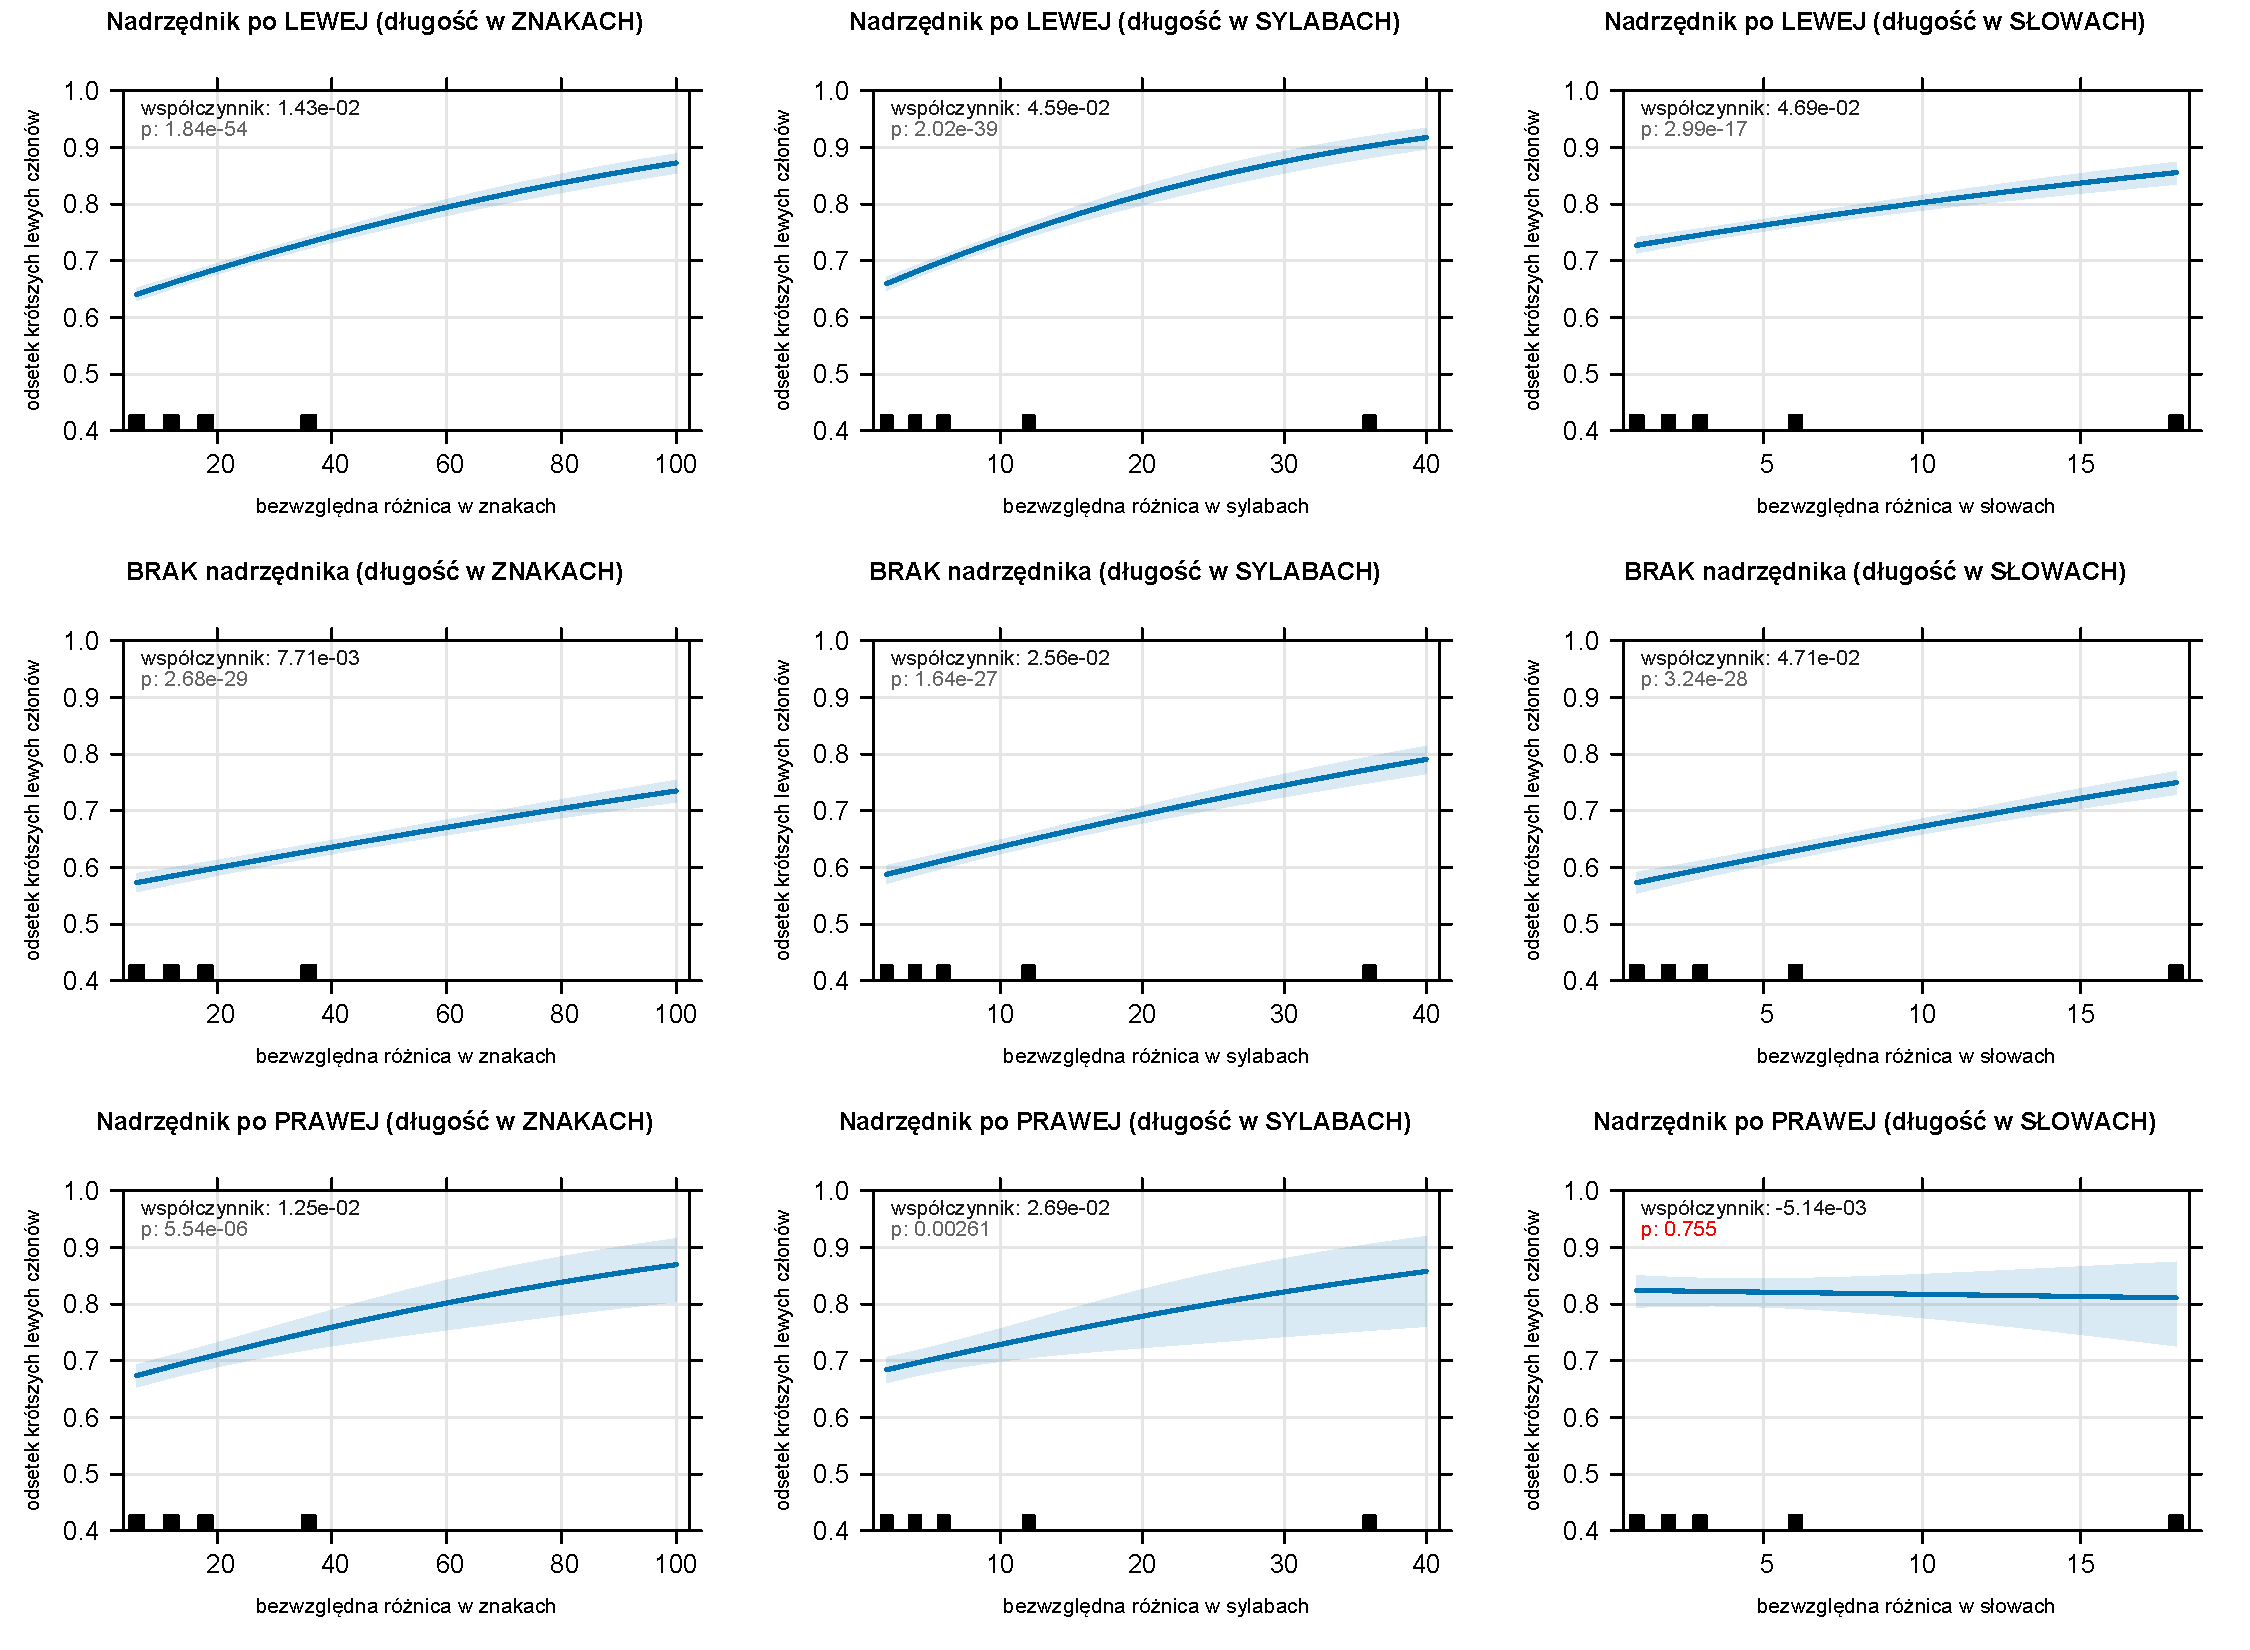
\includegraphics[scale=0.6]{English.pdf}
\caption{Różnica długości członów a występowanie krótszego członu po lewej stronie -- język \textbf{angielski}}
\label{fig:en}
\end{sidewaysfigure}

\begin{sidewaysfigure}
\centering
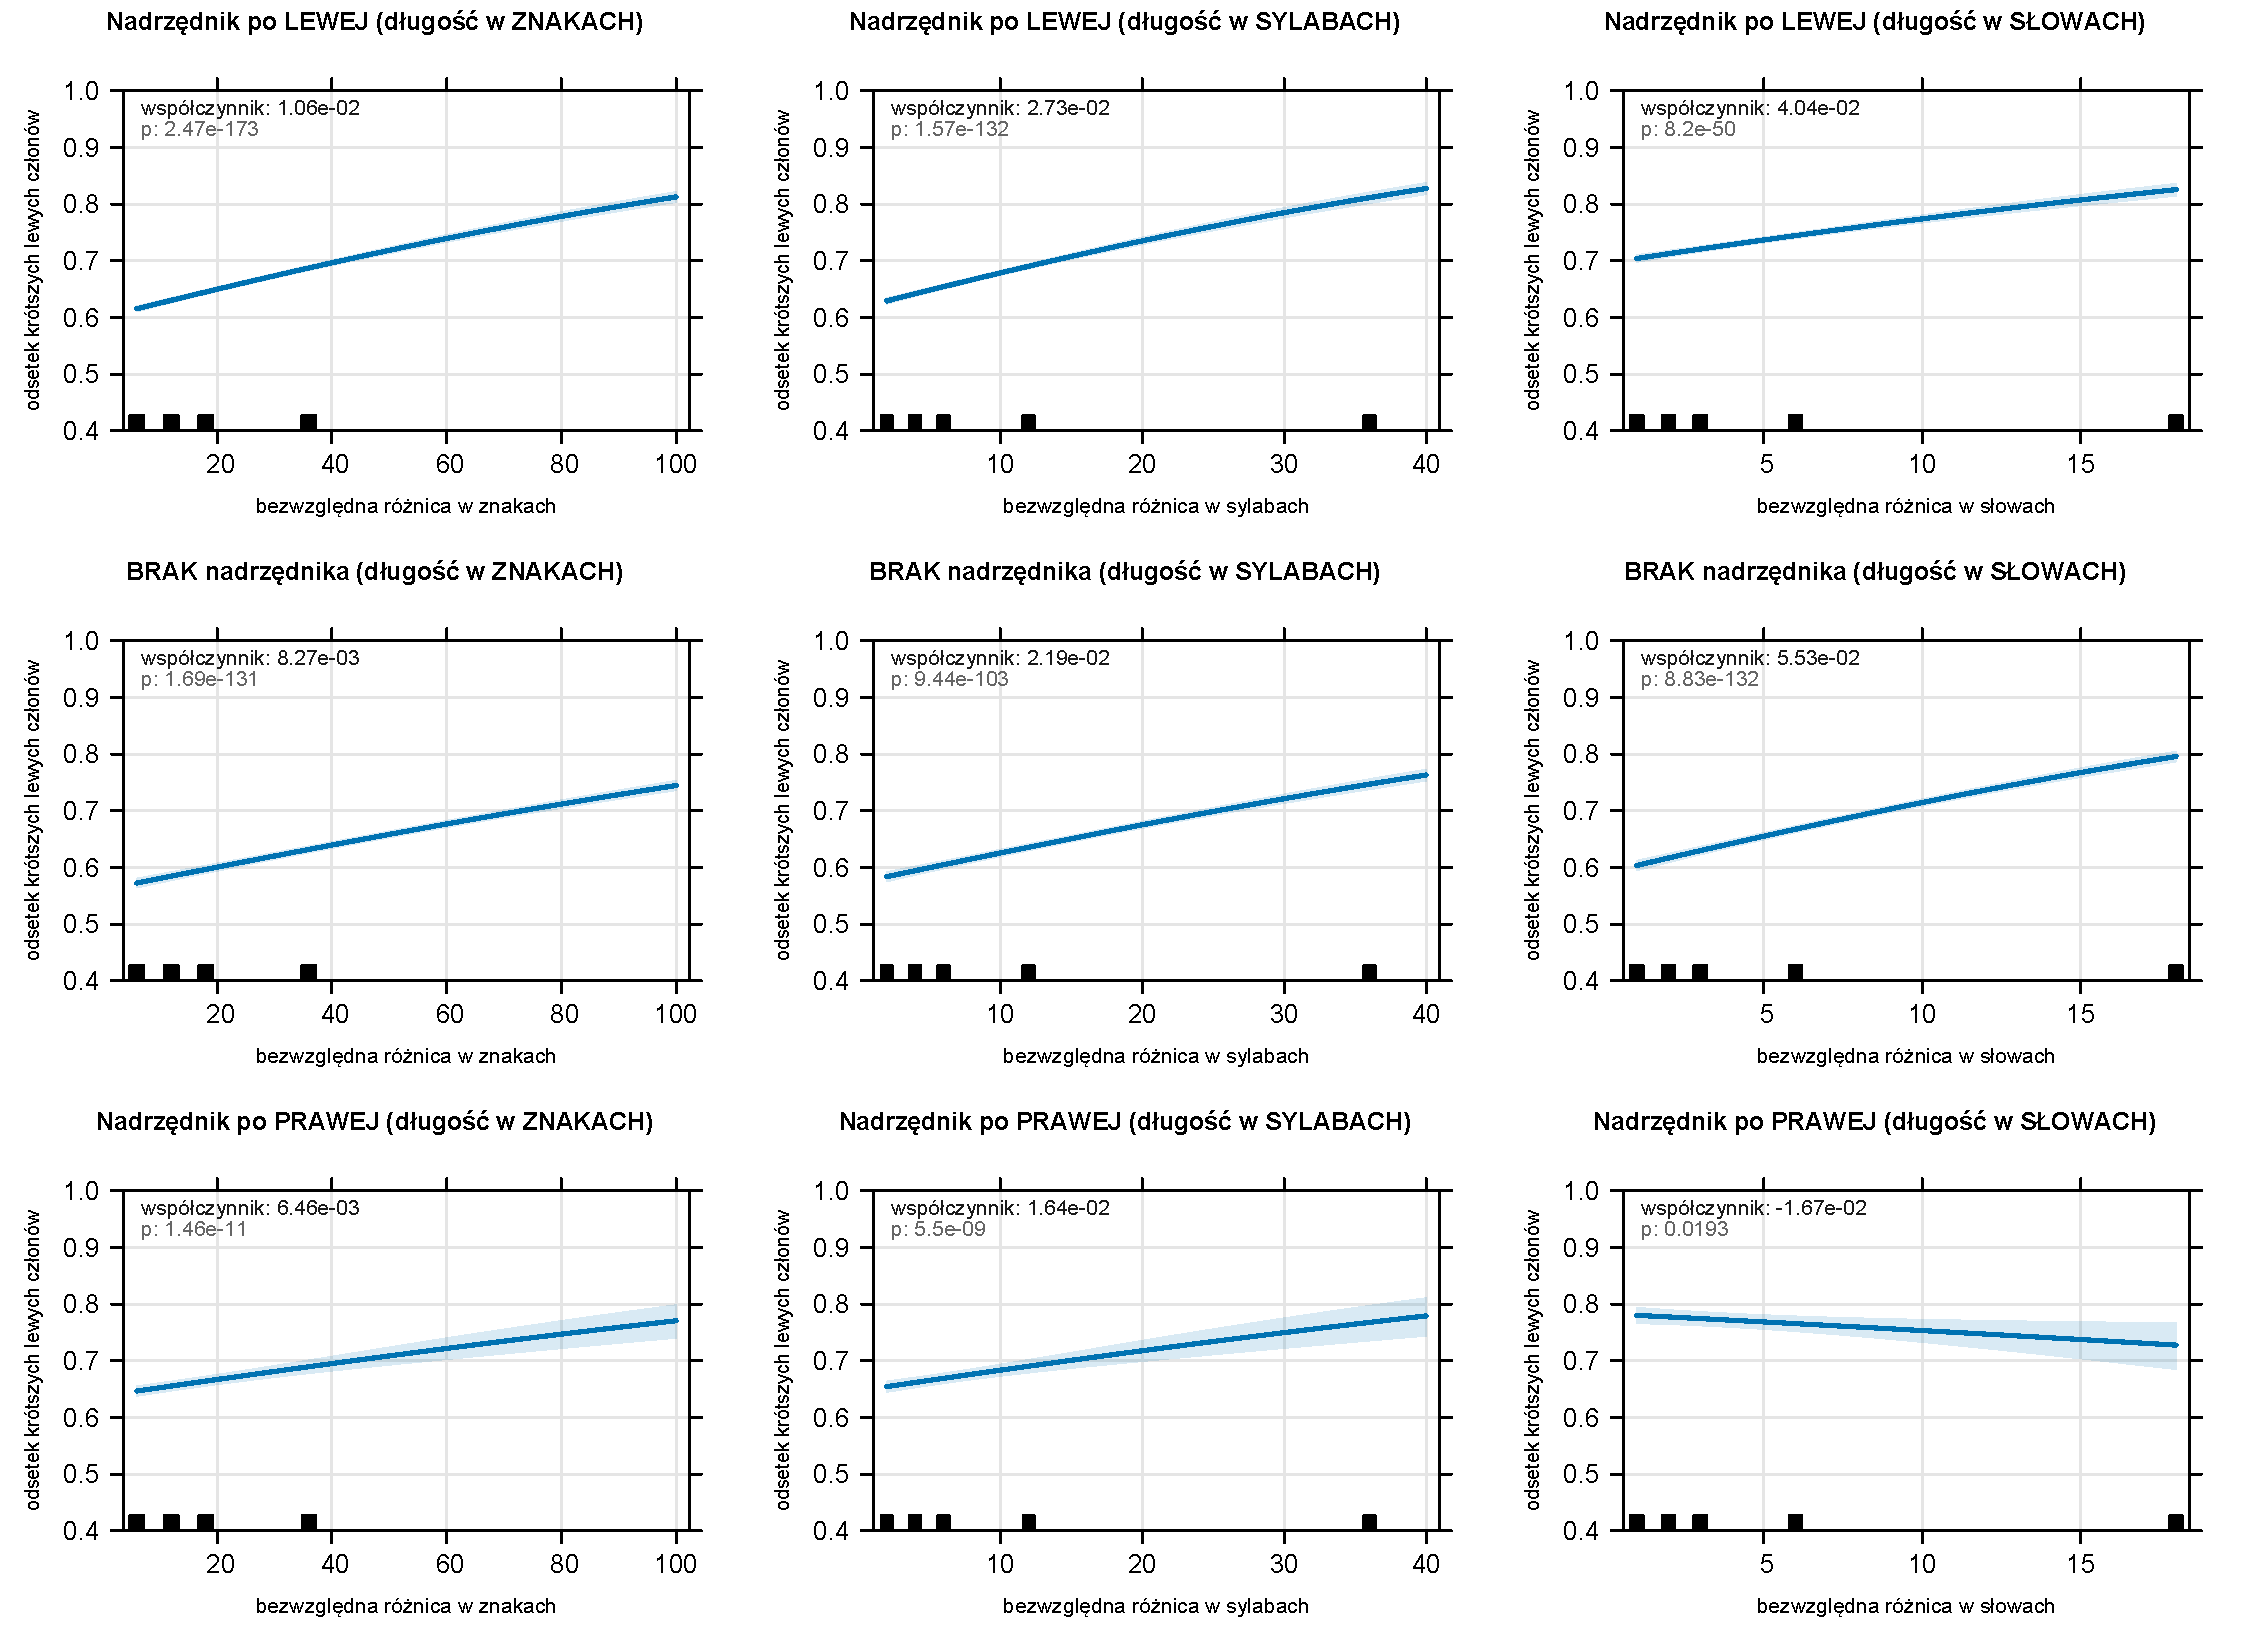
\includegraphics[scale=0.6]{Czech.pdf}
\caption{Różnica długości członów a występowanie krótszego członu po lewej stronie -- język \textbf{czeski}}
\label{fig:cz}
\end{sidewaysfigure}

\begin{sidewaysfigure}
\centering
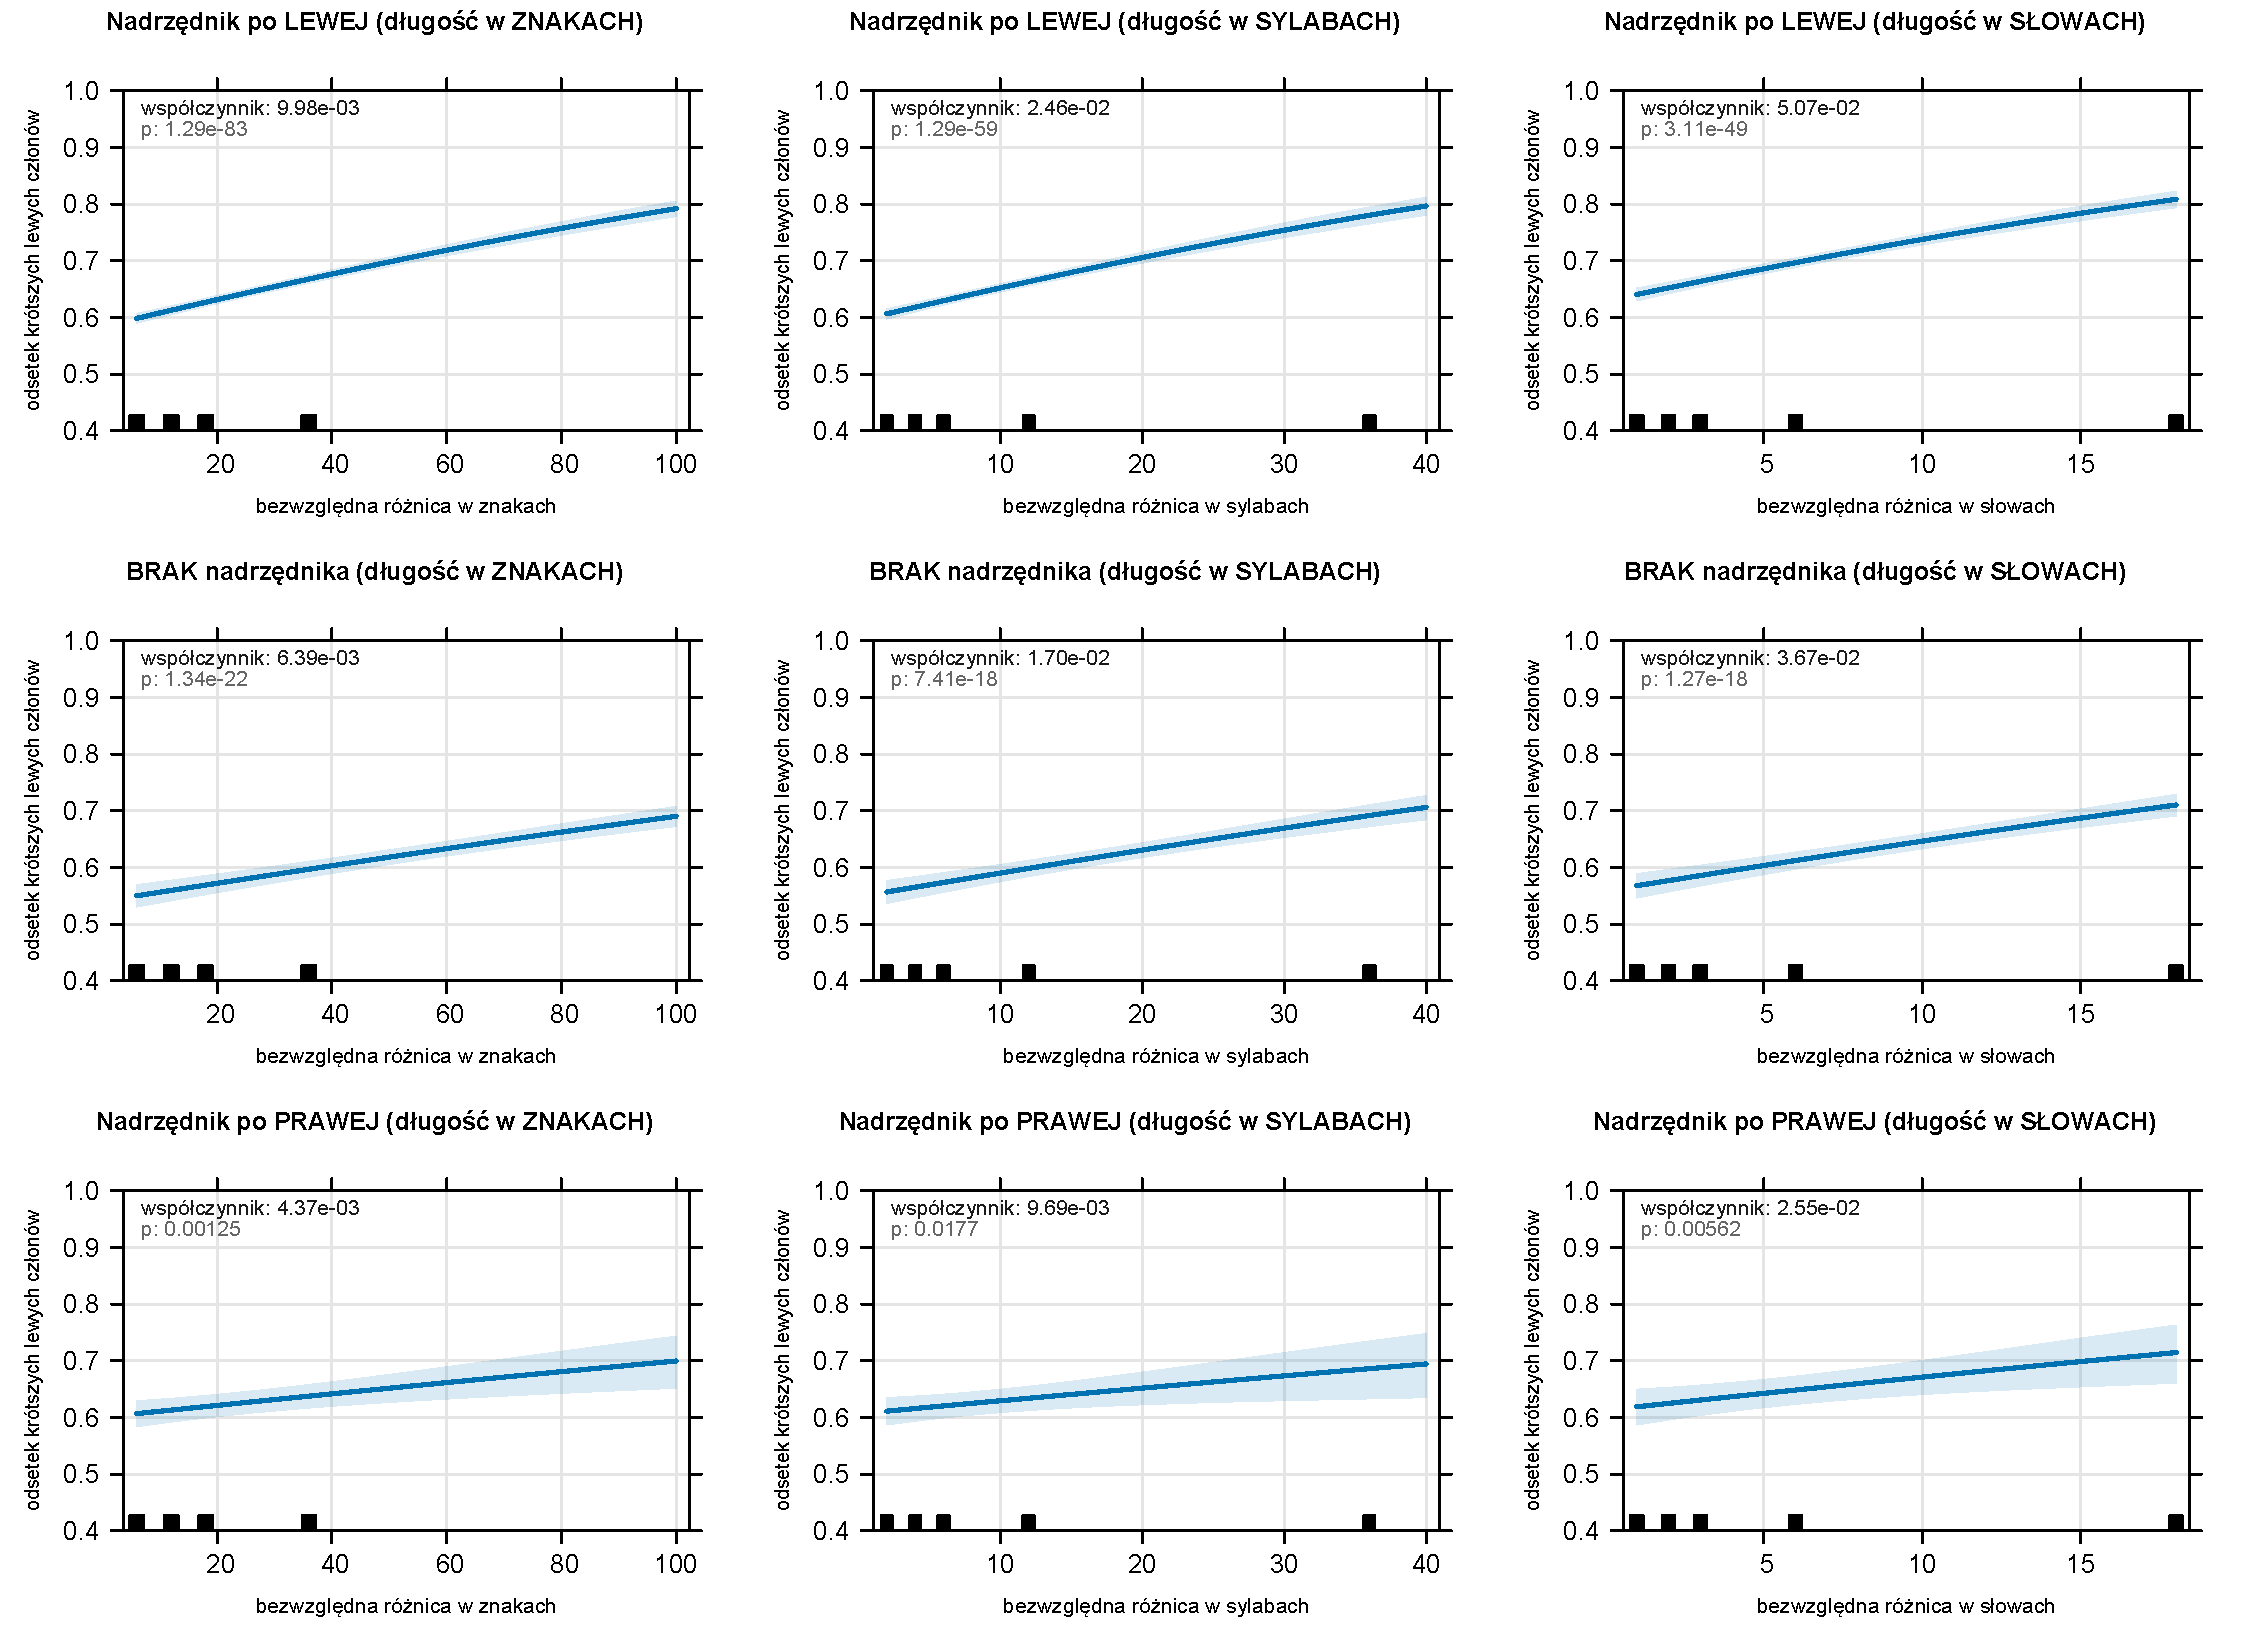
\includegraphics[scale=0.6]{Spanish.pdf}
\caption{Różnica długości członów a występowanie krótszego członu po lewej stronie -- język \textbf{hiszpański}}
\label{fig:es}
\end{sidewaysfigure}

\begin{sidewaysfigure}
\centering
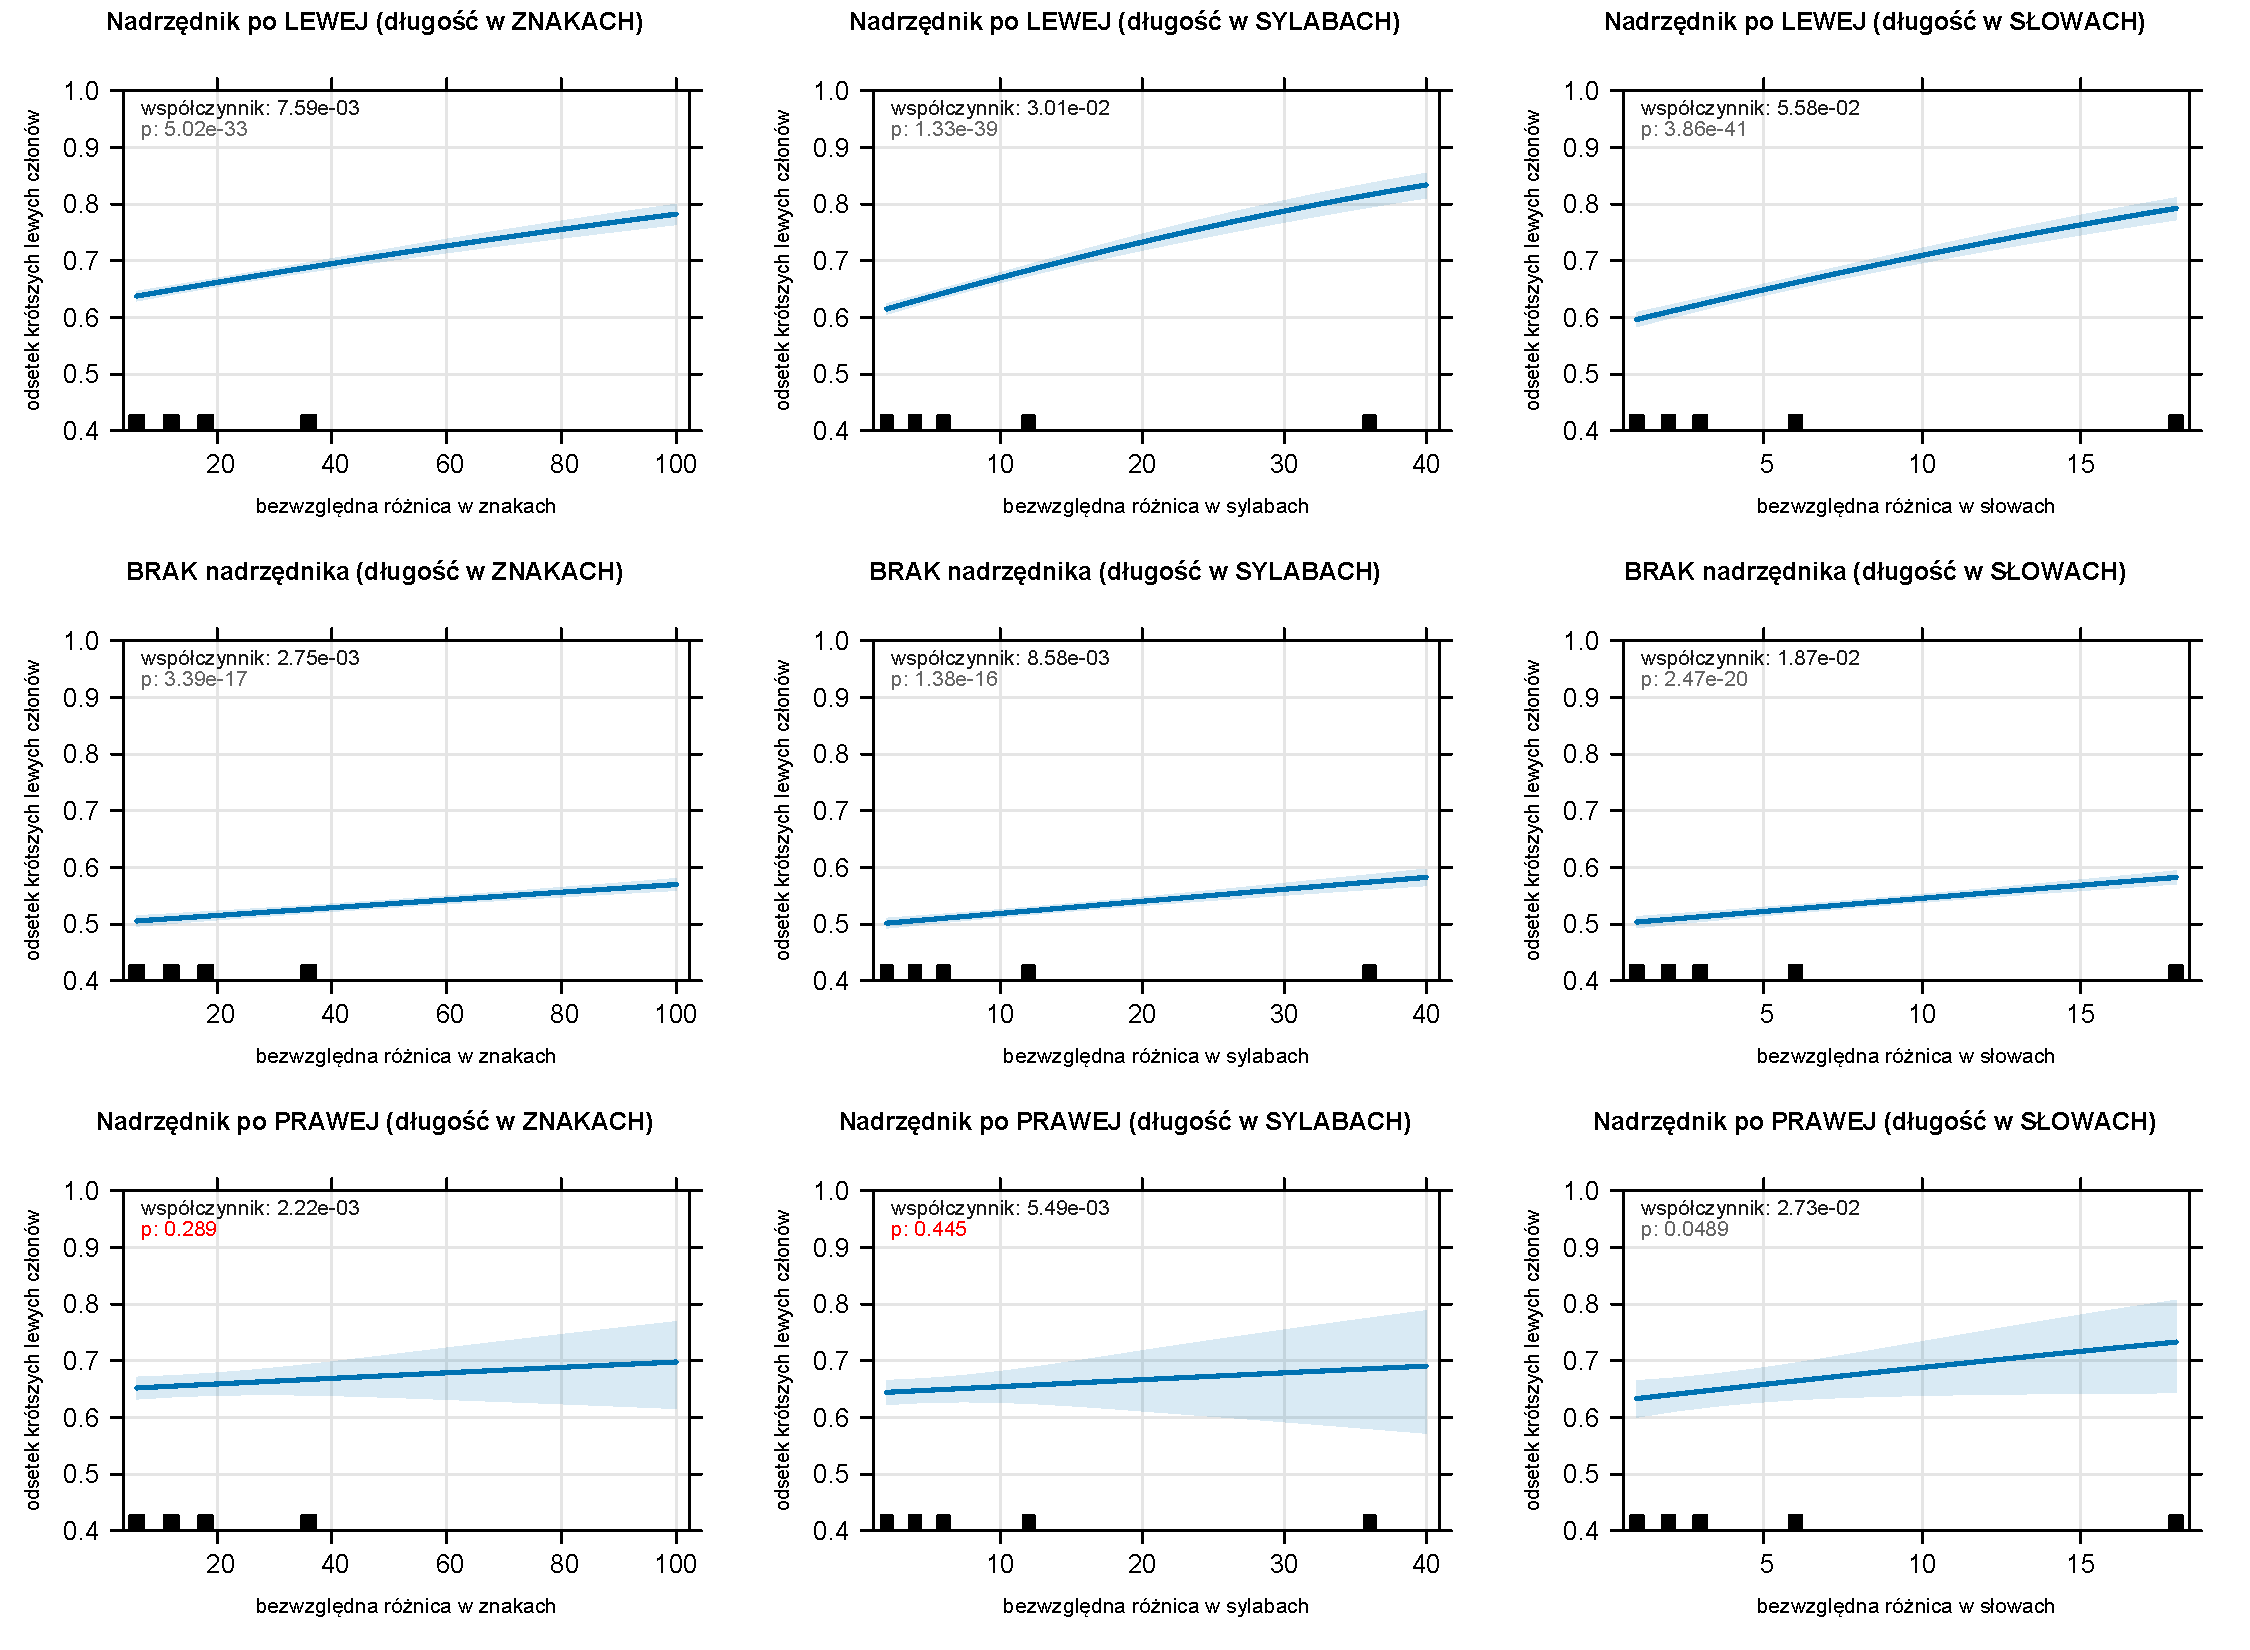
\includegraphics[scale=0.6]{Icelandic.pdf}
\caption{Różnica długości członów a występowanie krótszego członu po lewej stronie -- język \textbf{islandzki}}
\label{fig:is}
\end{sidewaysfigure}

\begin{sidewaysfigure}
\centering
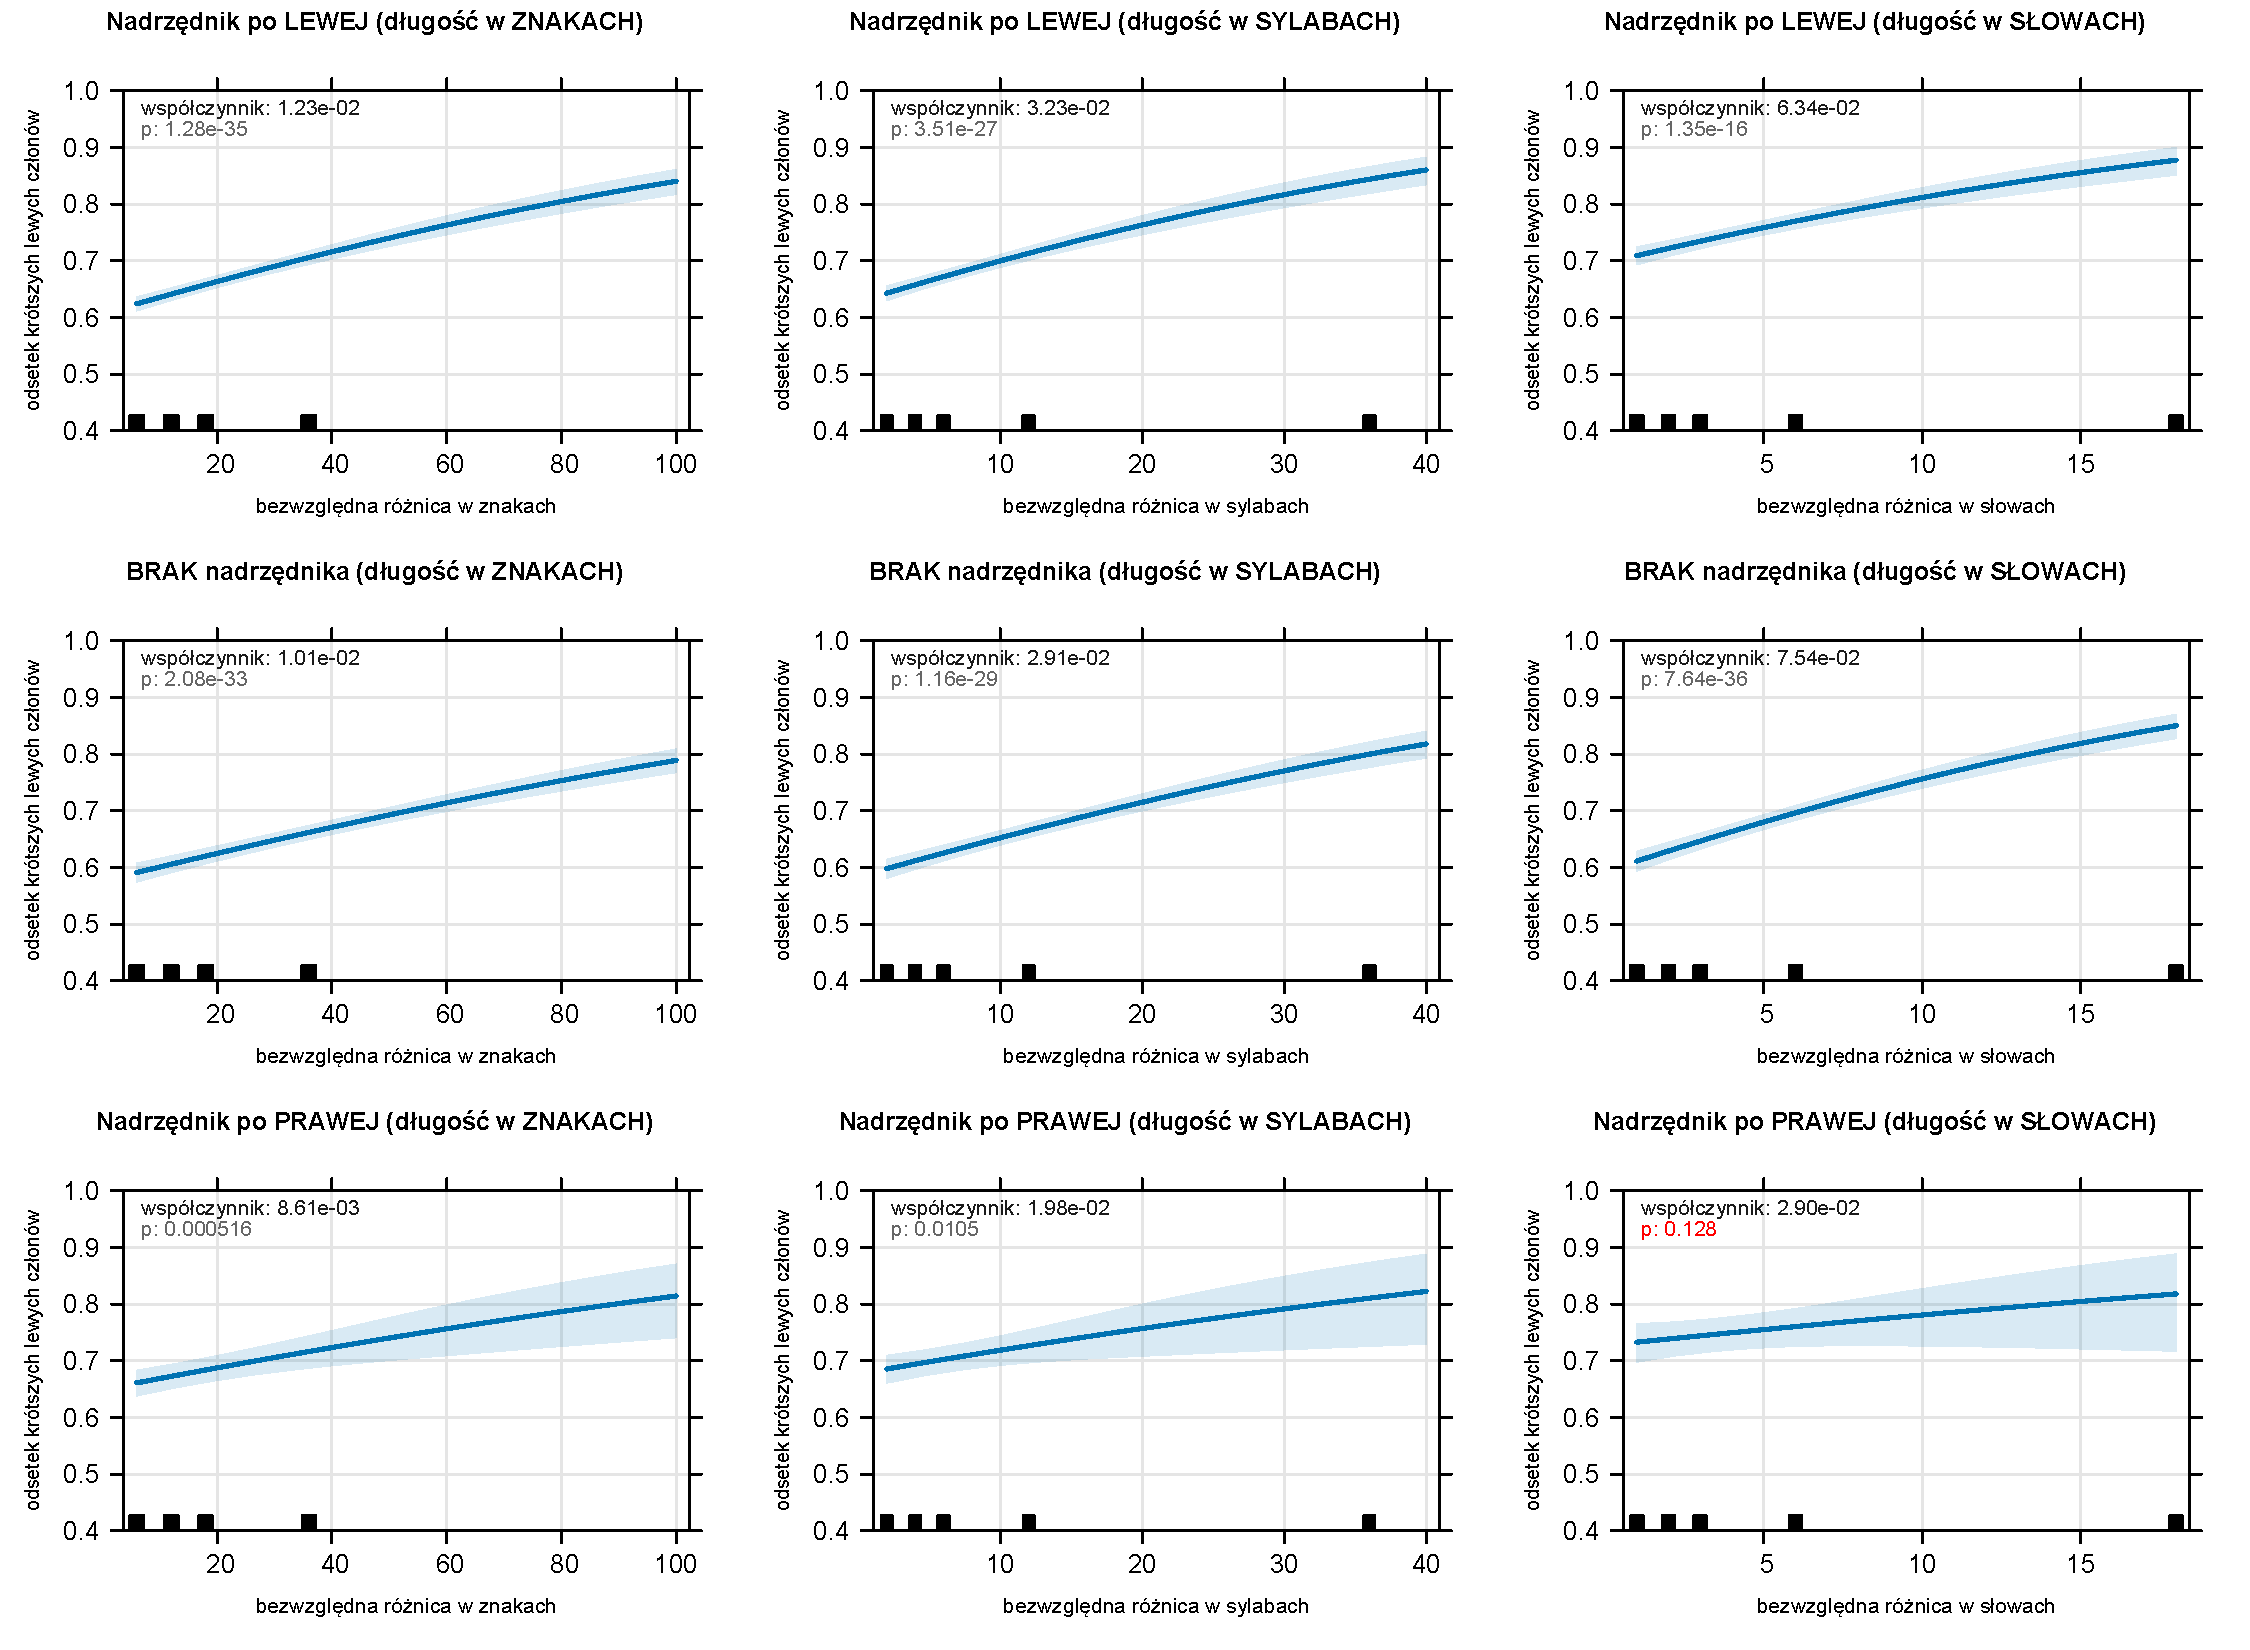
\includegraphics[scale=0.6]{Polish.pdf}
\caption{Różnica długości członów a występowanie krótszego członu po lewej stronie -- język \textbf{polski}}
\label{fig:pl}
\end{sidewaysfigure}

\begin{sidewaysfigure}
\centering
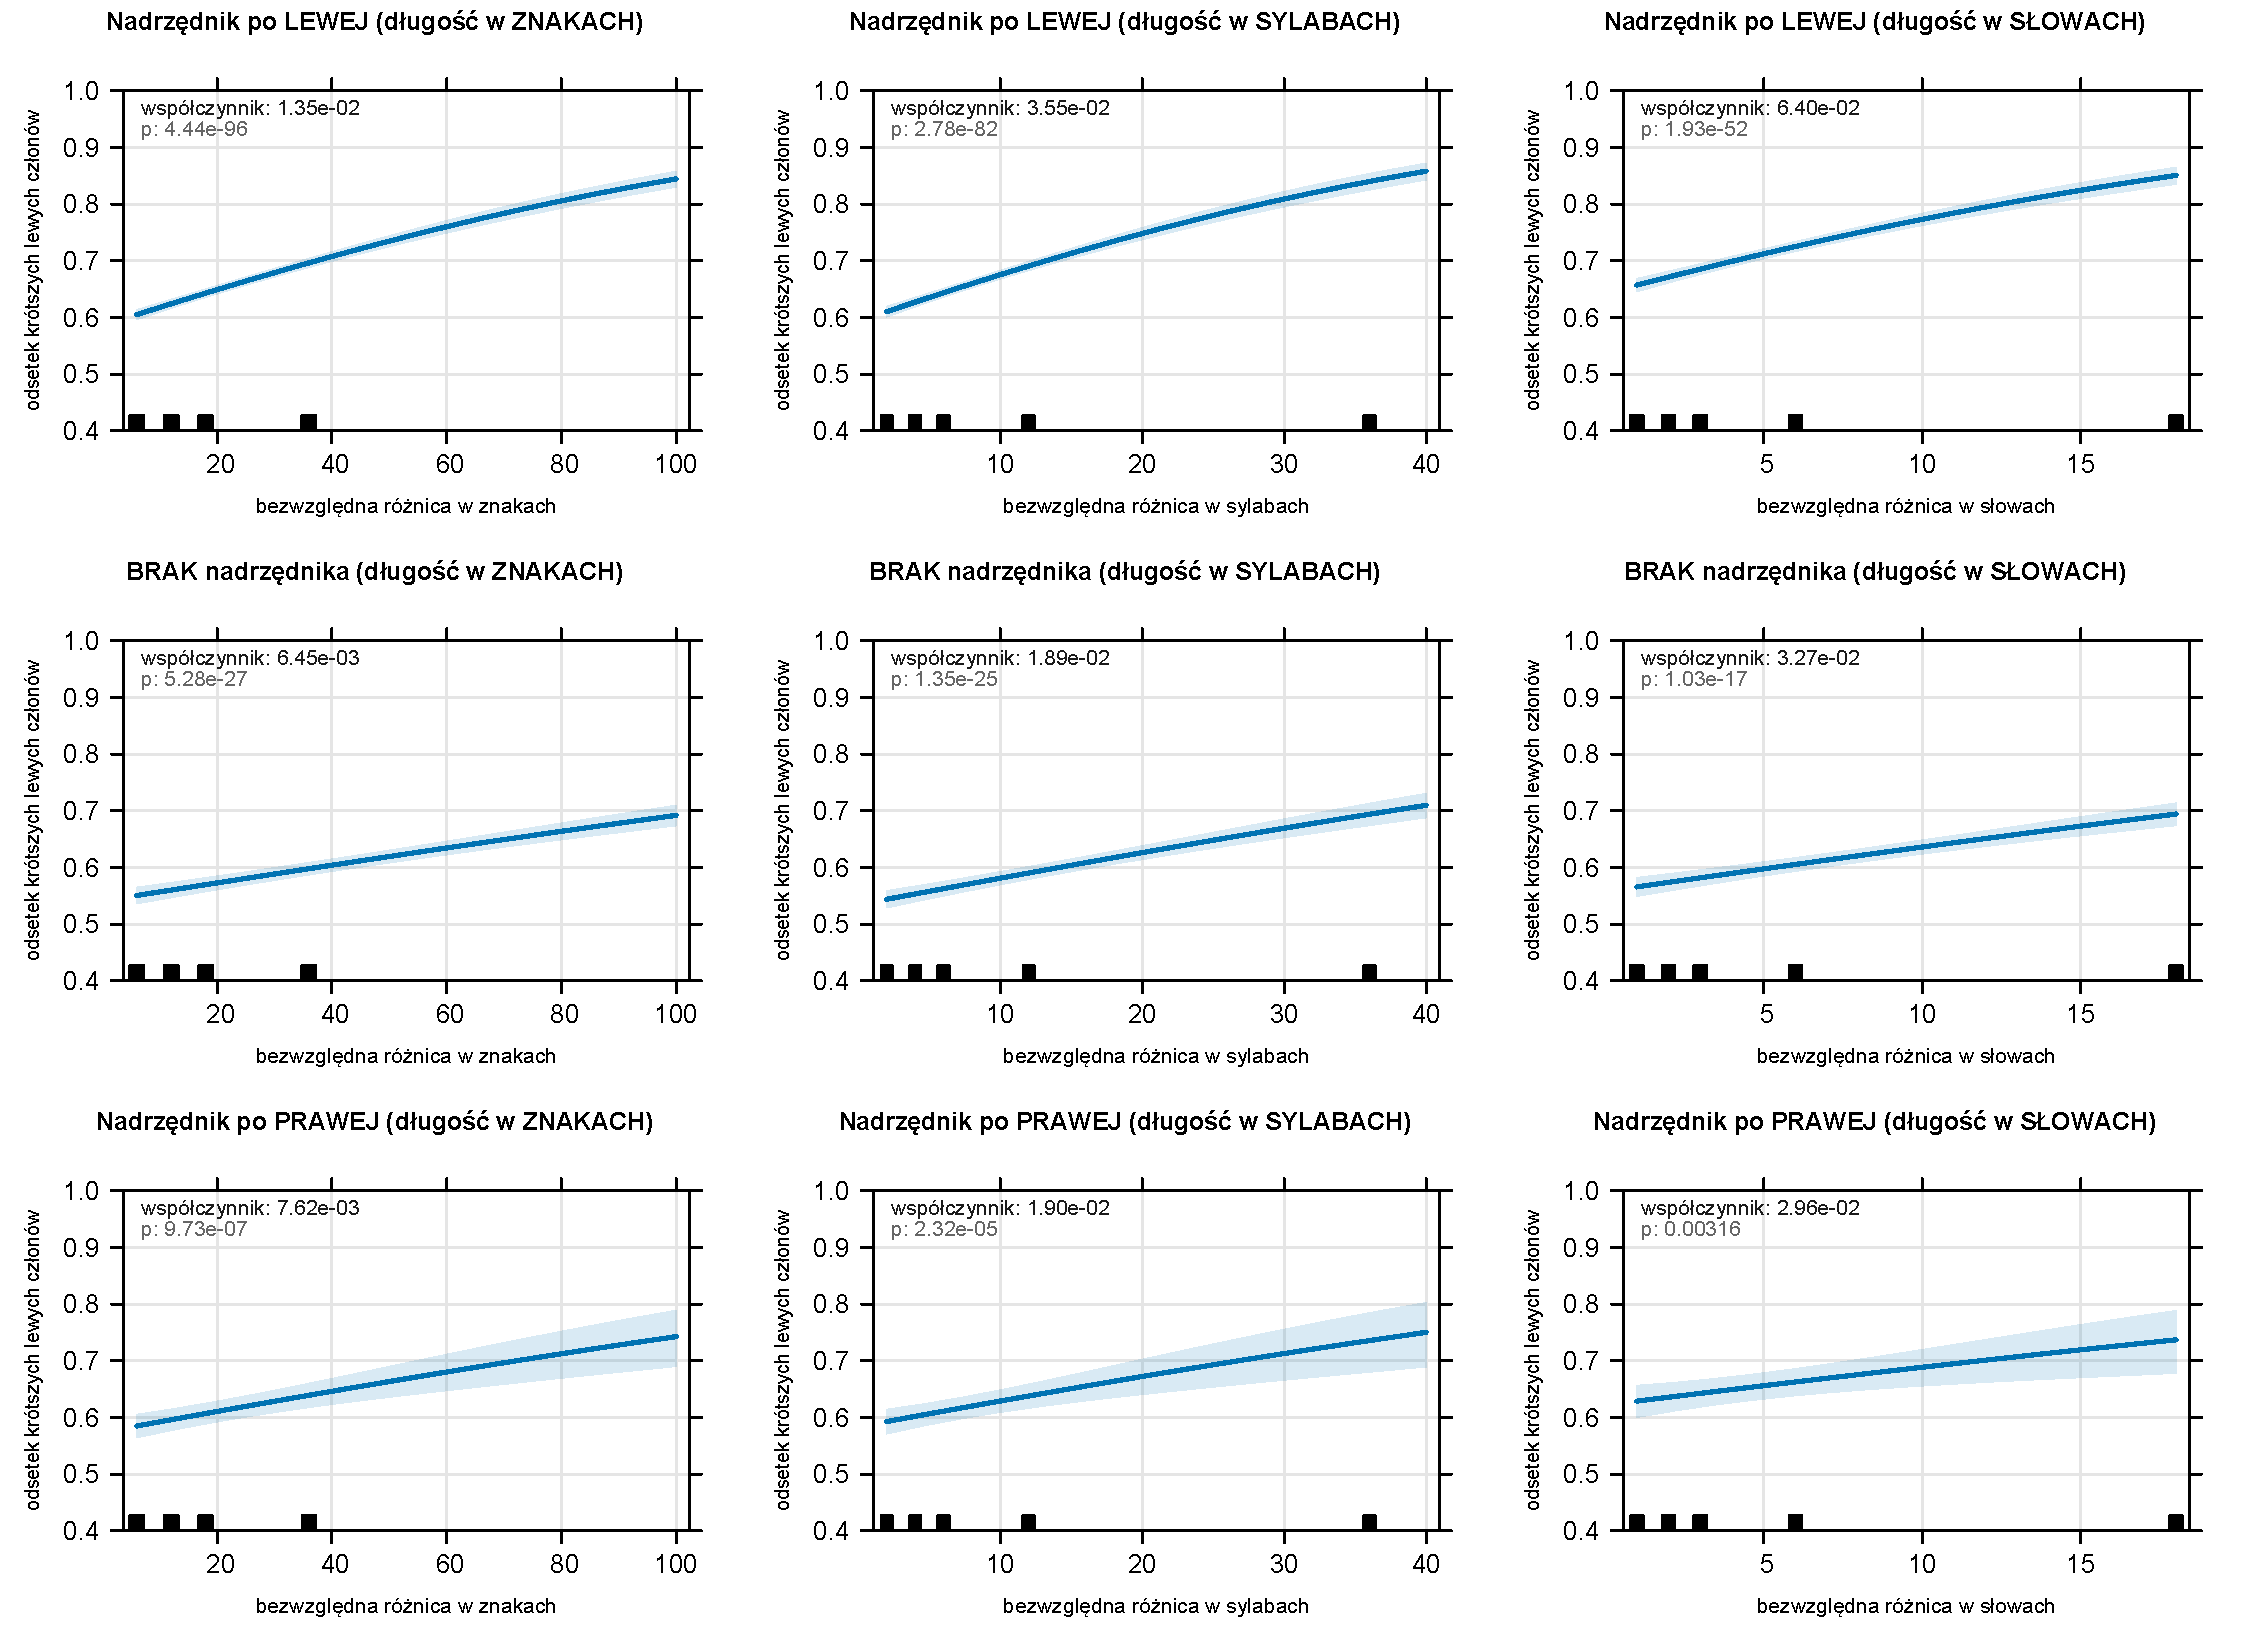
\includegraphics[scale=0.6]{Portuguese.pdf}
\caption{Różnica długości członów a występowanie krótszego członu po lewej stronie -- język \textbf{portugalski}}
\label{fig:po}
\end{sidewaysfigure}

\begin{sidewaysfigure}
\centering
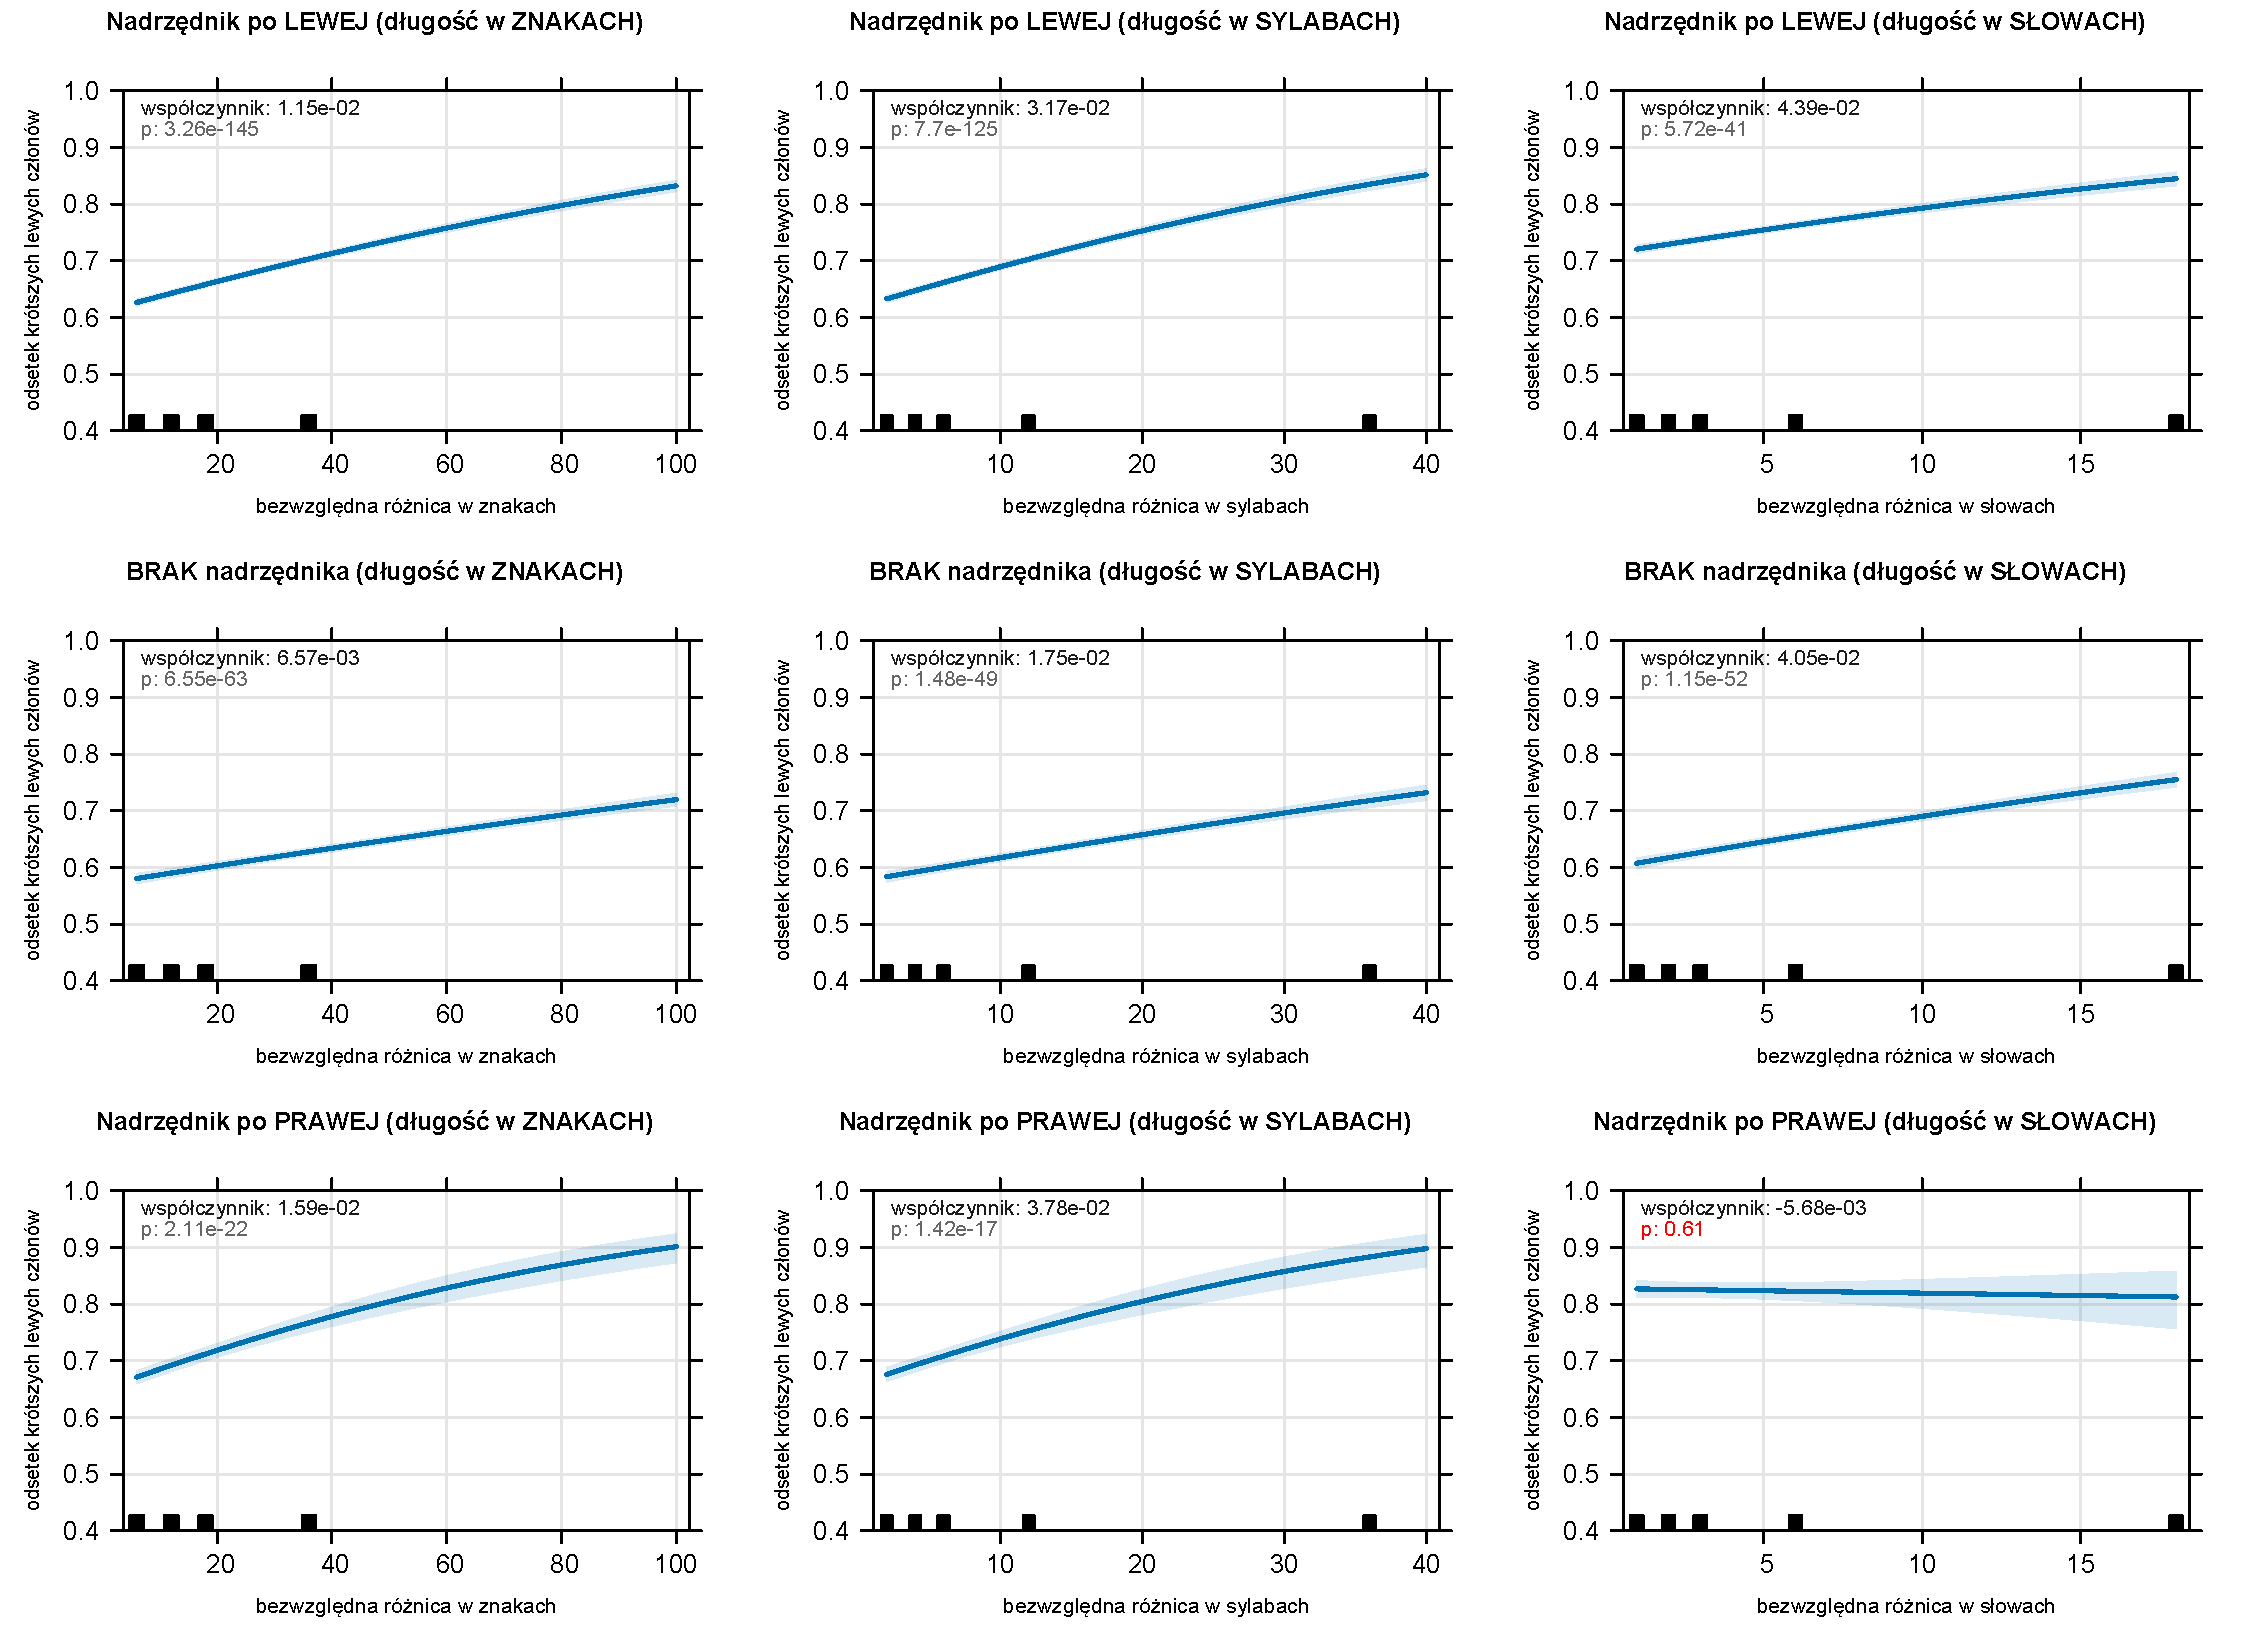
\includegraphics[scale=0.6]{Russian.pdf}
\caption{Różnica długości członów a występowanie krótszego członu po lewej stronie -- język \textbf{rosyjski}}
\label{fig:ru}
\end{sidewaysfigure}

\begin{sidewaysfigure}
\centering
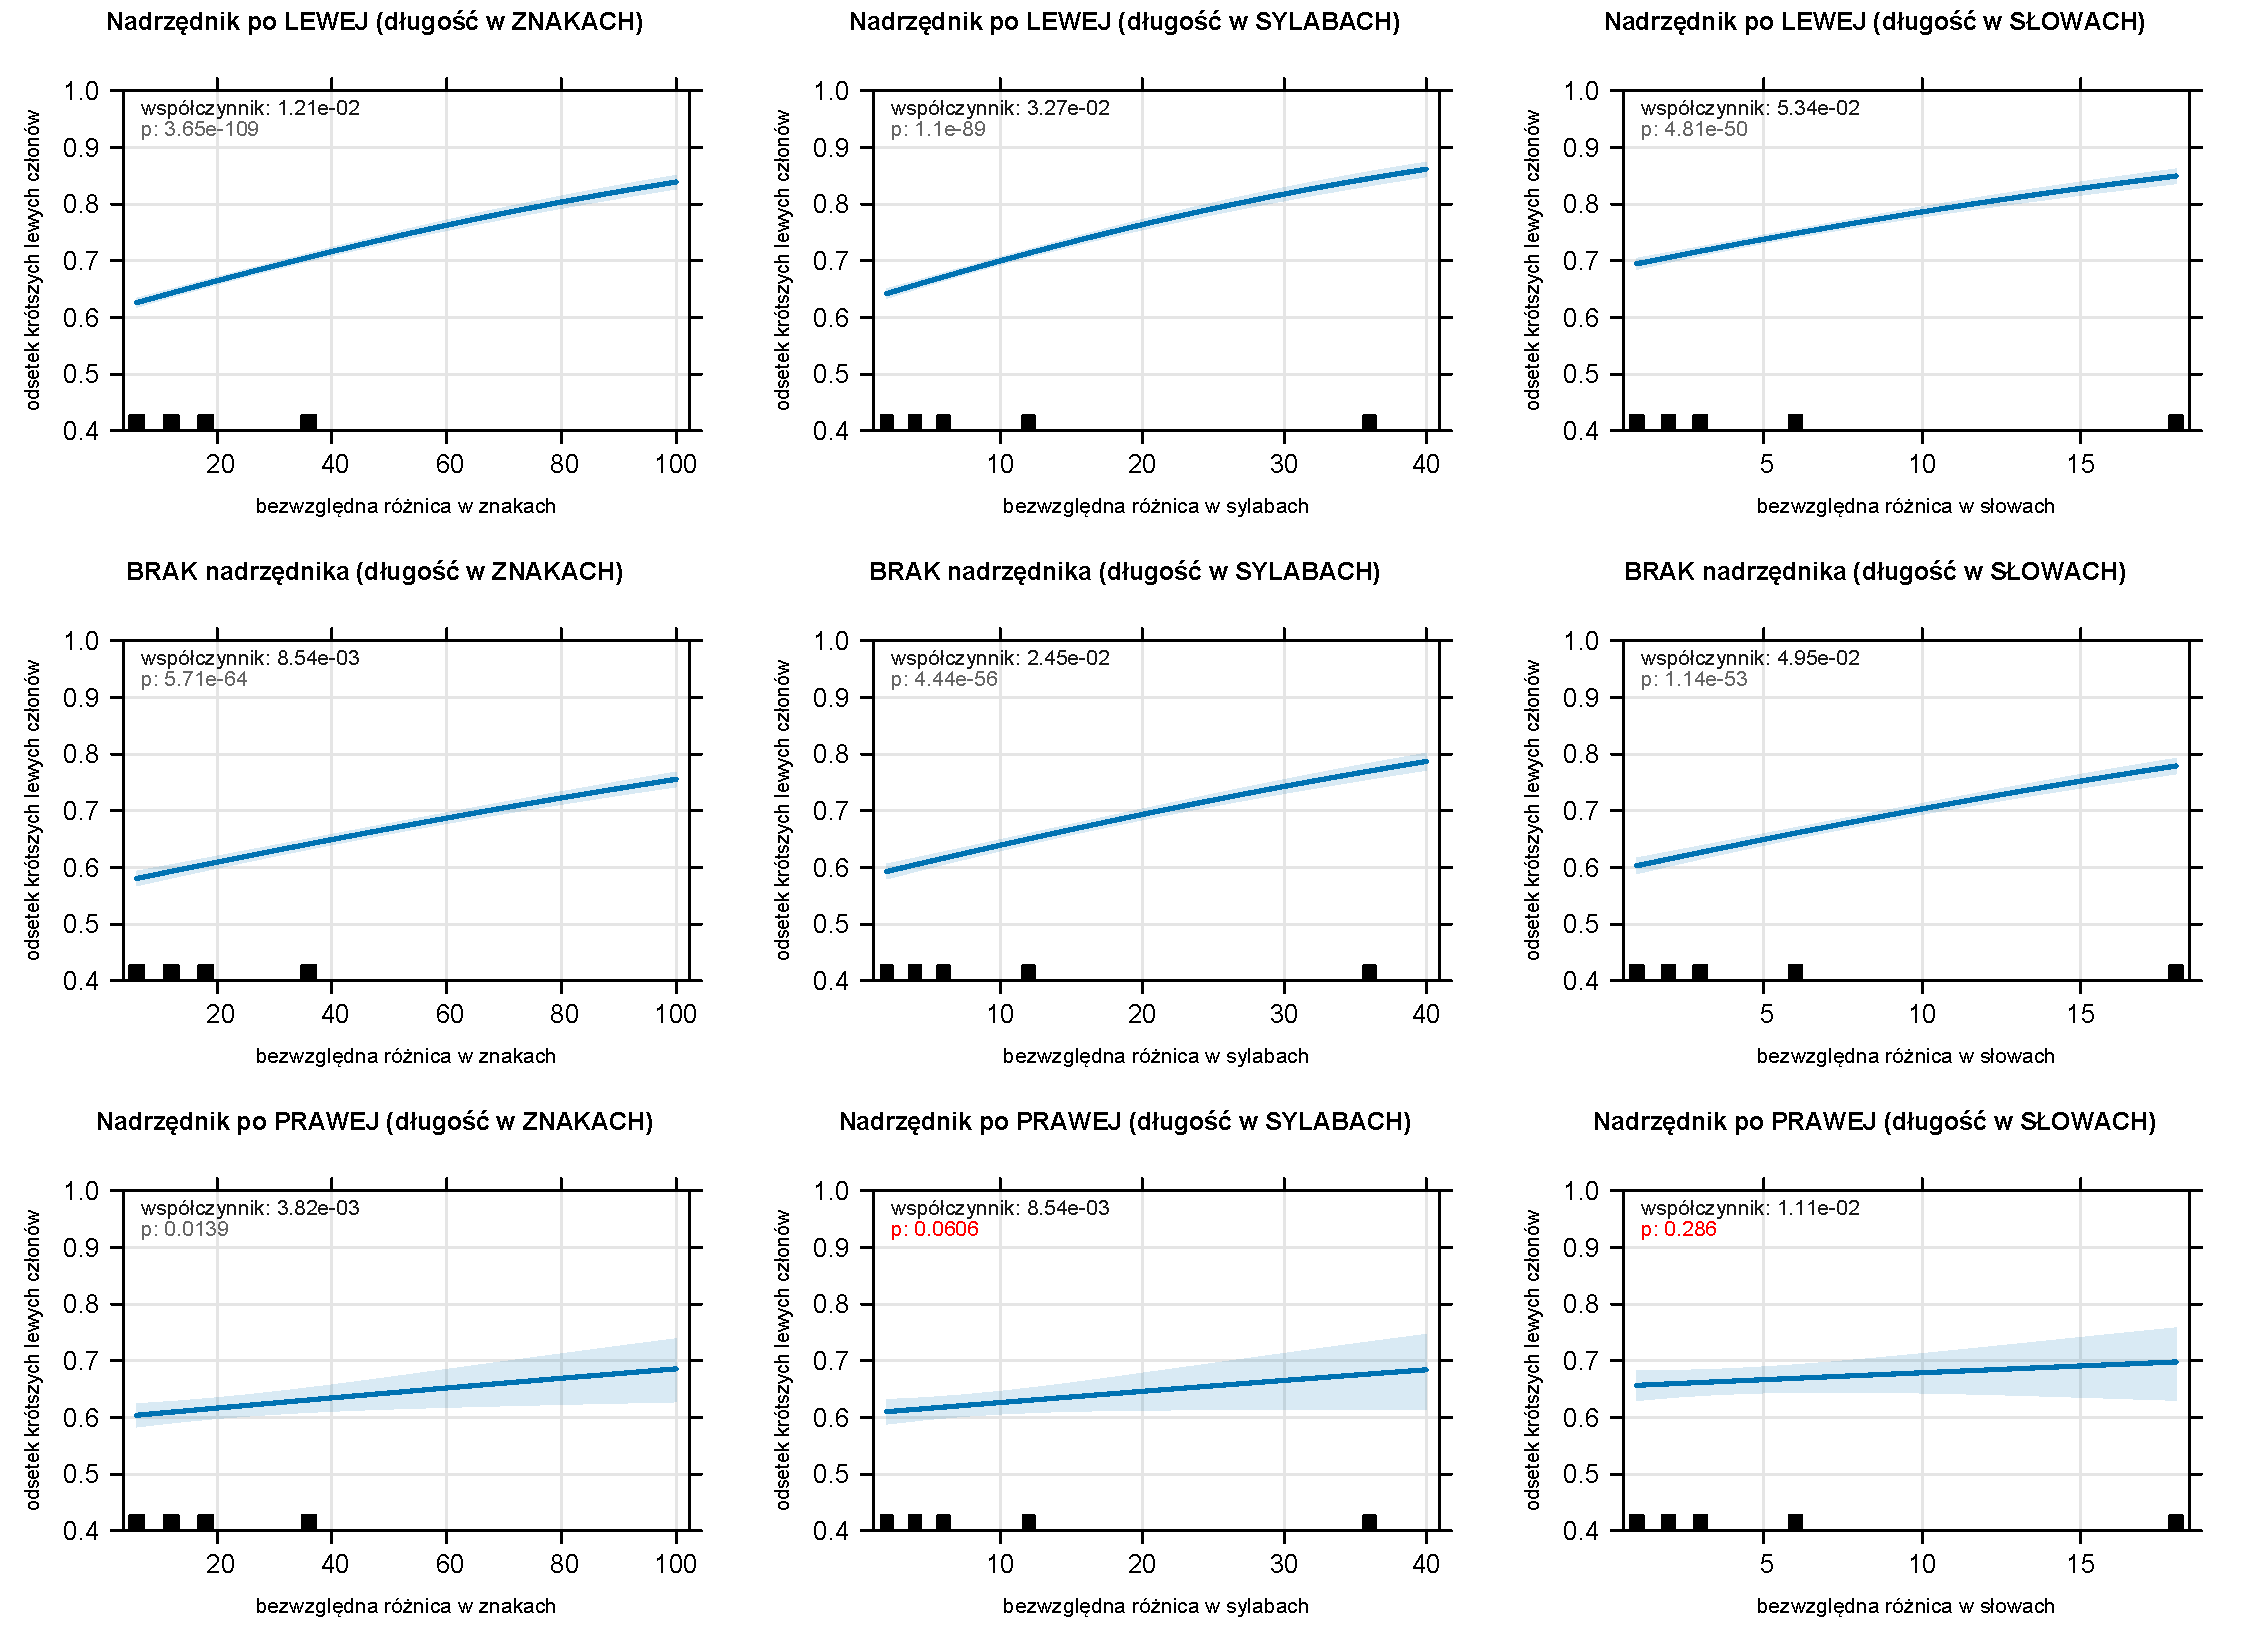
\includegraphics[scale=0.6]{Romanian.pdf}
\caption{Różnica długości członów a występowanie krótszego członu po lewej stronie -- język \textbf{rumuński}}
\label{fig:ro}
\end{sidewaysfigure}

\begin{sidewaysfigure}
\centering
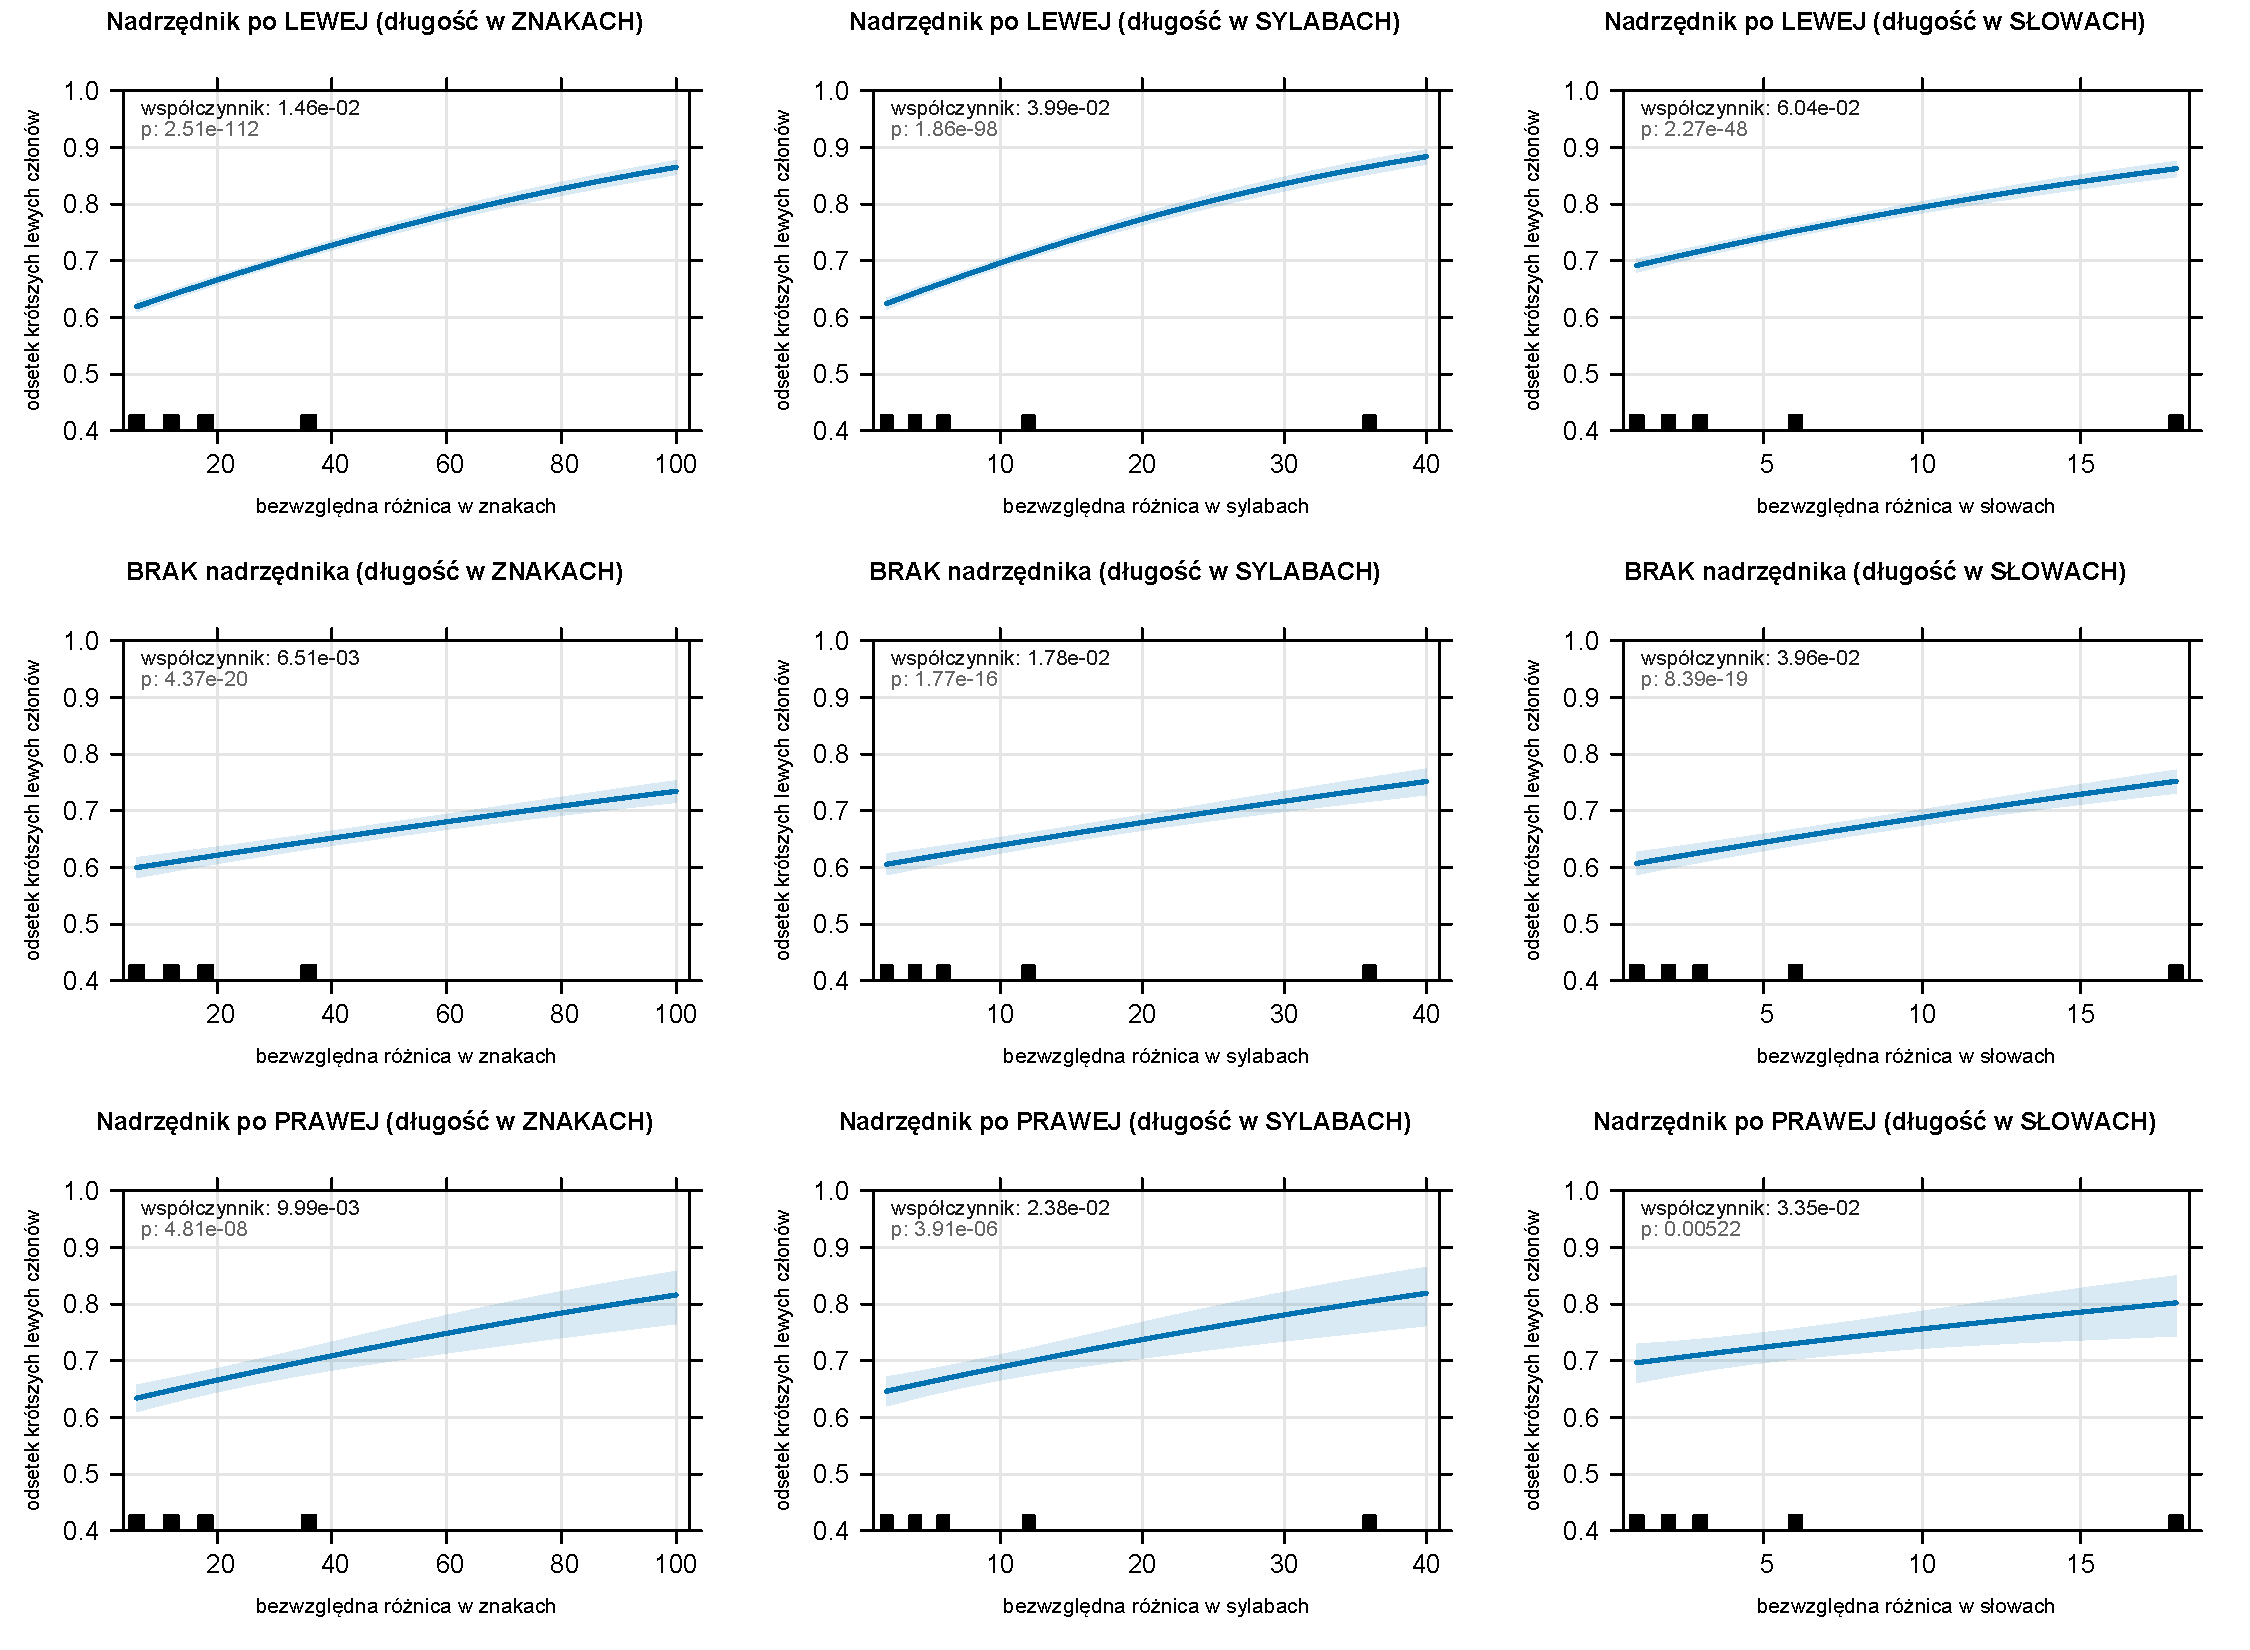
\includegraphics[scale=0.6]{Italian.pdf}
\caption{Różnica długości członów a występowanie krótszego członu po lewej stronie -- język \textbf{włoski}}
\label{fig:it}
\end{sidewaysfigure}

\newpage

\section{Języki mieszane}

\begin{sidewaysfigure}
\centering
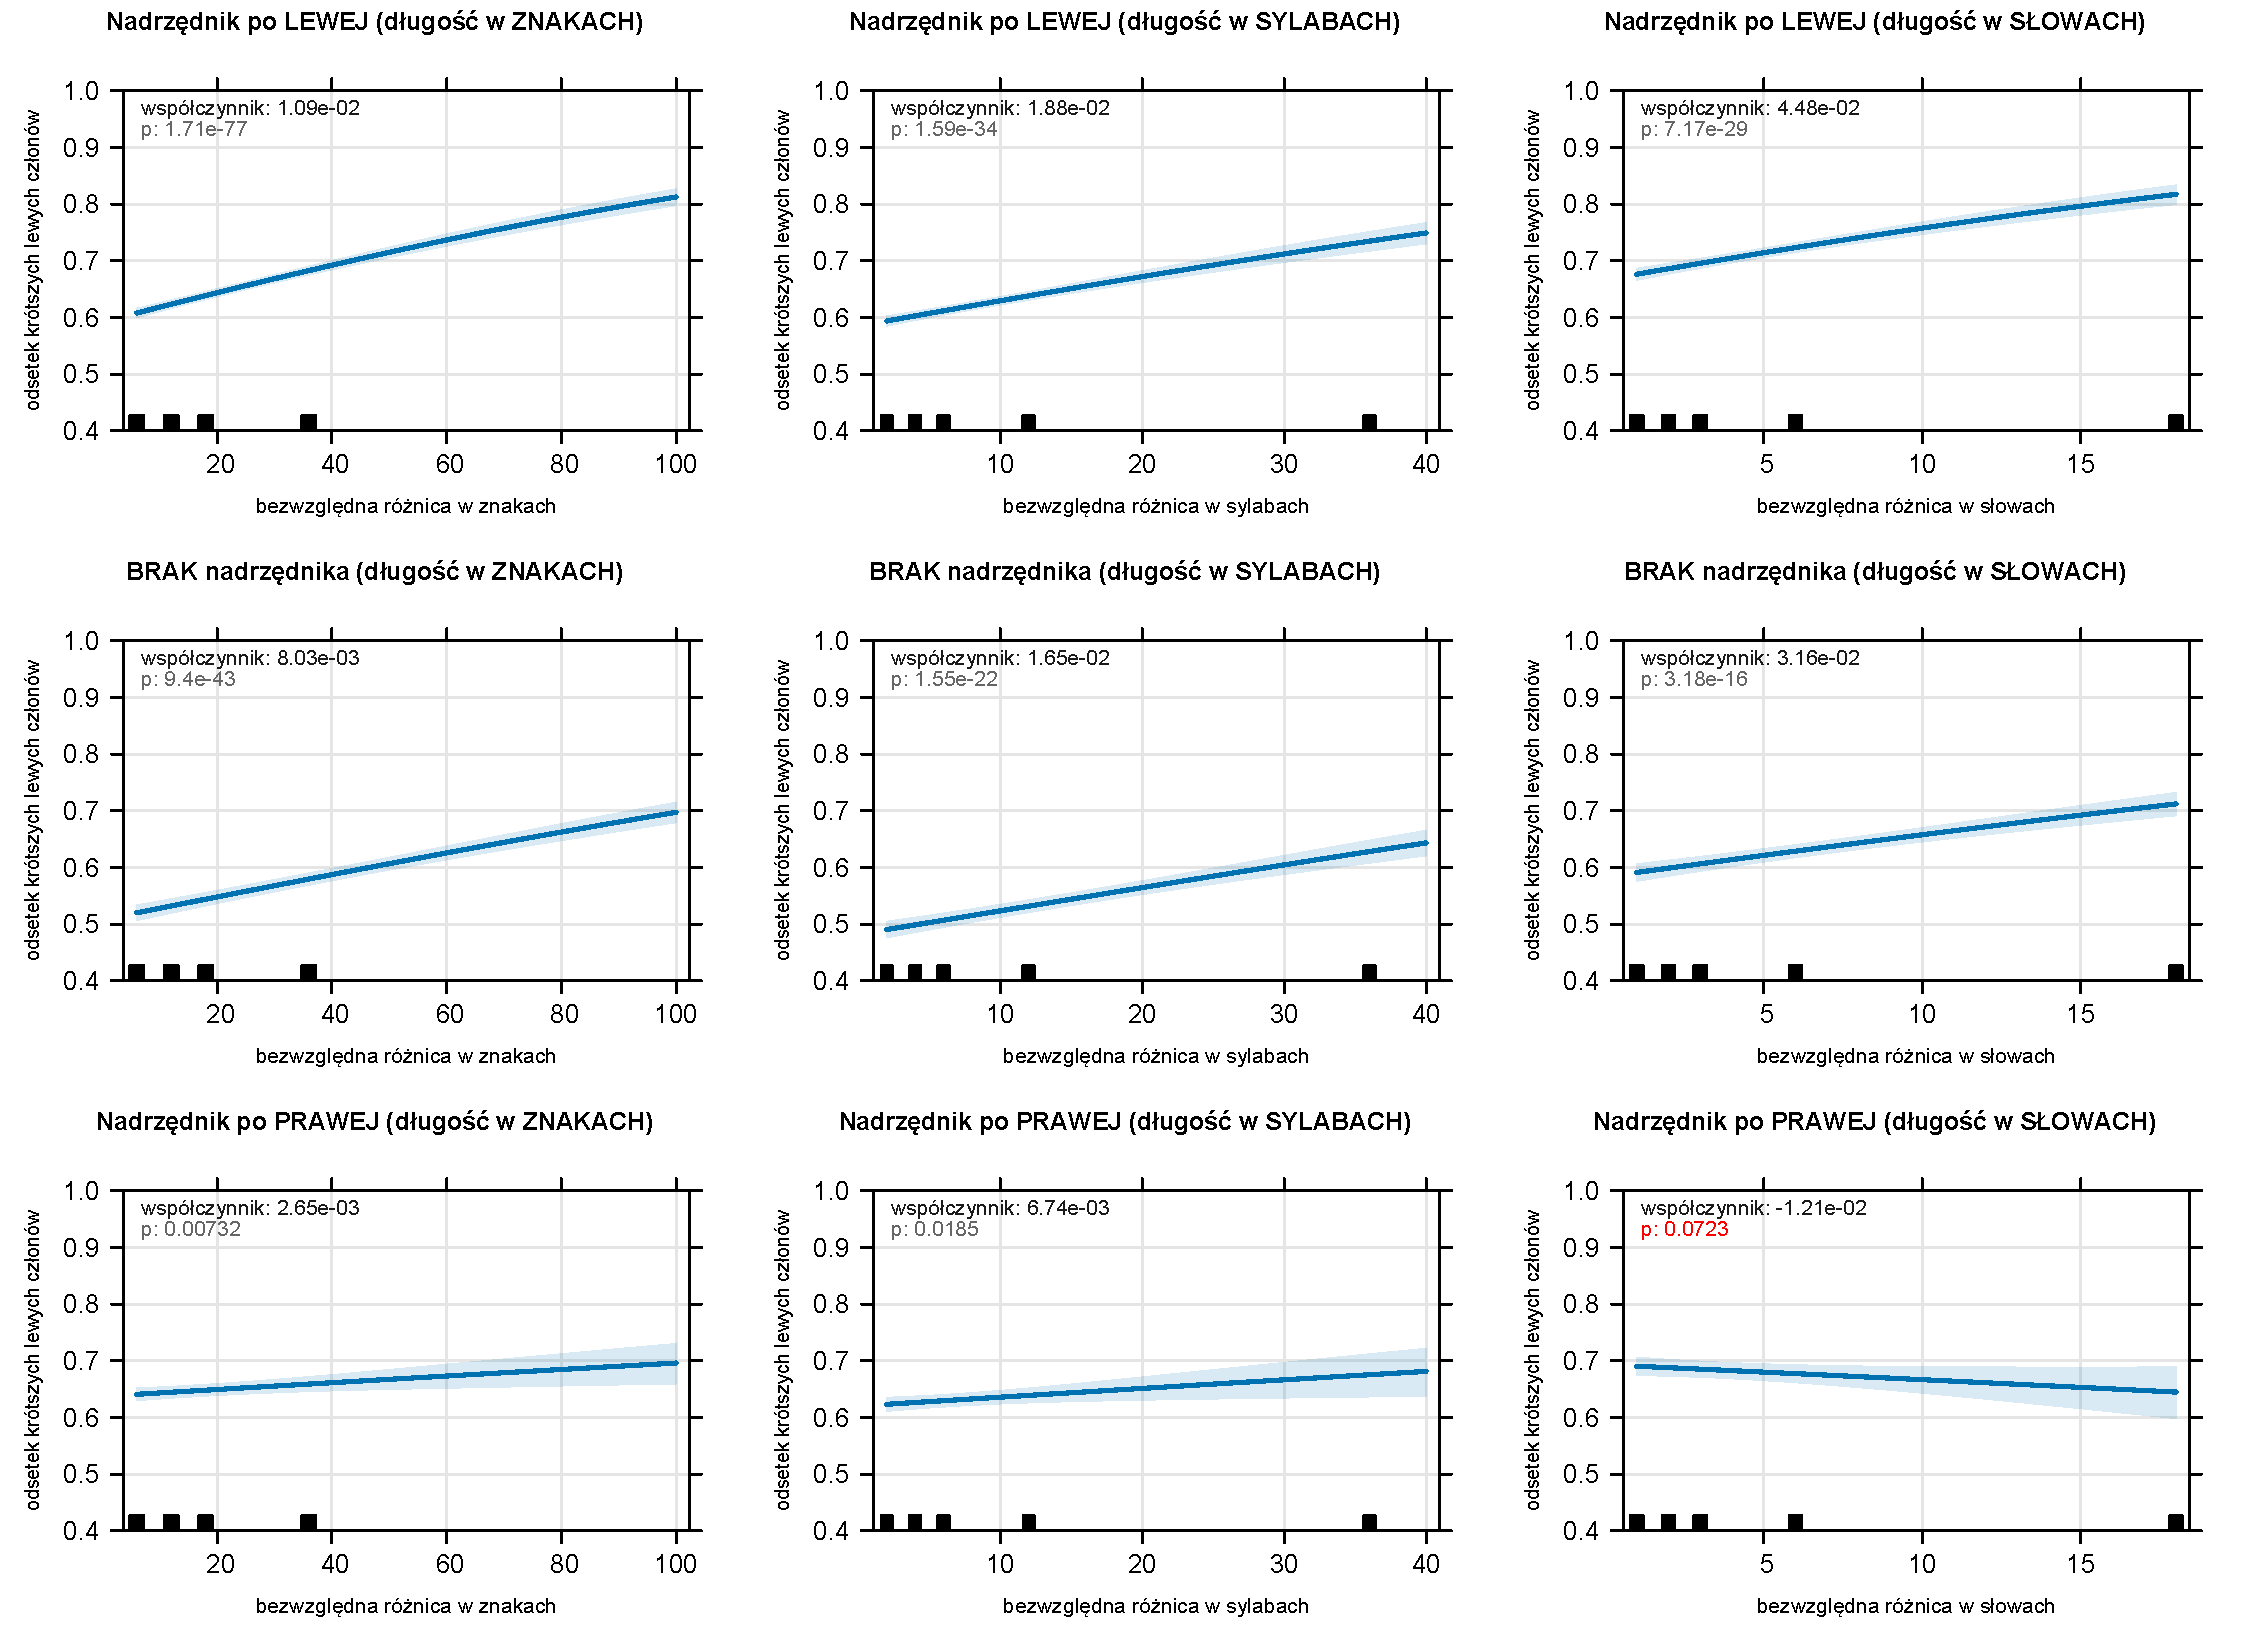
\includegraphics[scale=0.6]{Latin.pdf}
\caption{Różnica długości członów a występowanie krótszego członu po lewej stronie -- język \textbf{łaciński}}
\label{fig:la}
\end{sidewaysfigure}

\begin{sidewaysfigure}
\centering
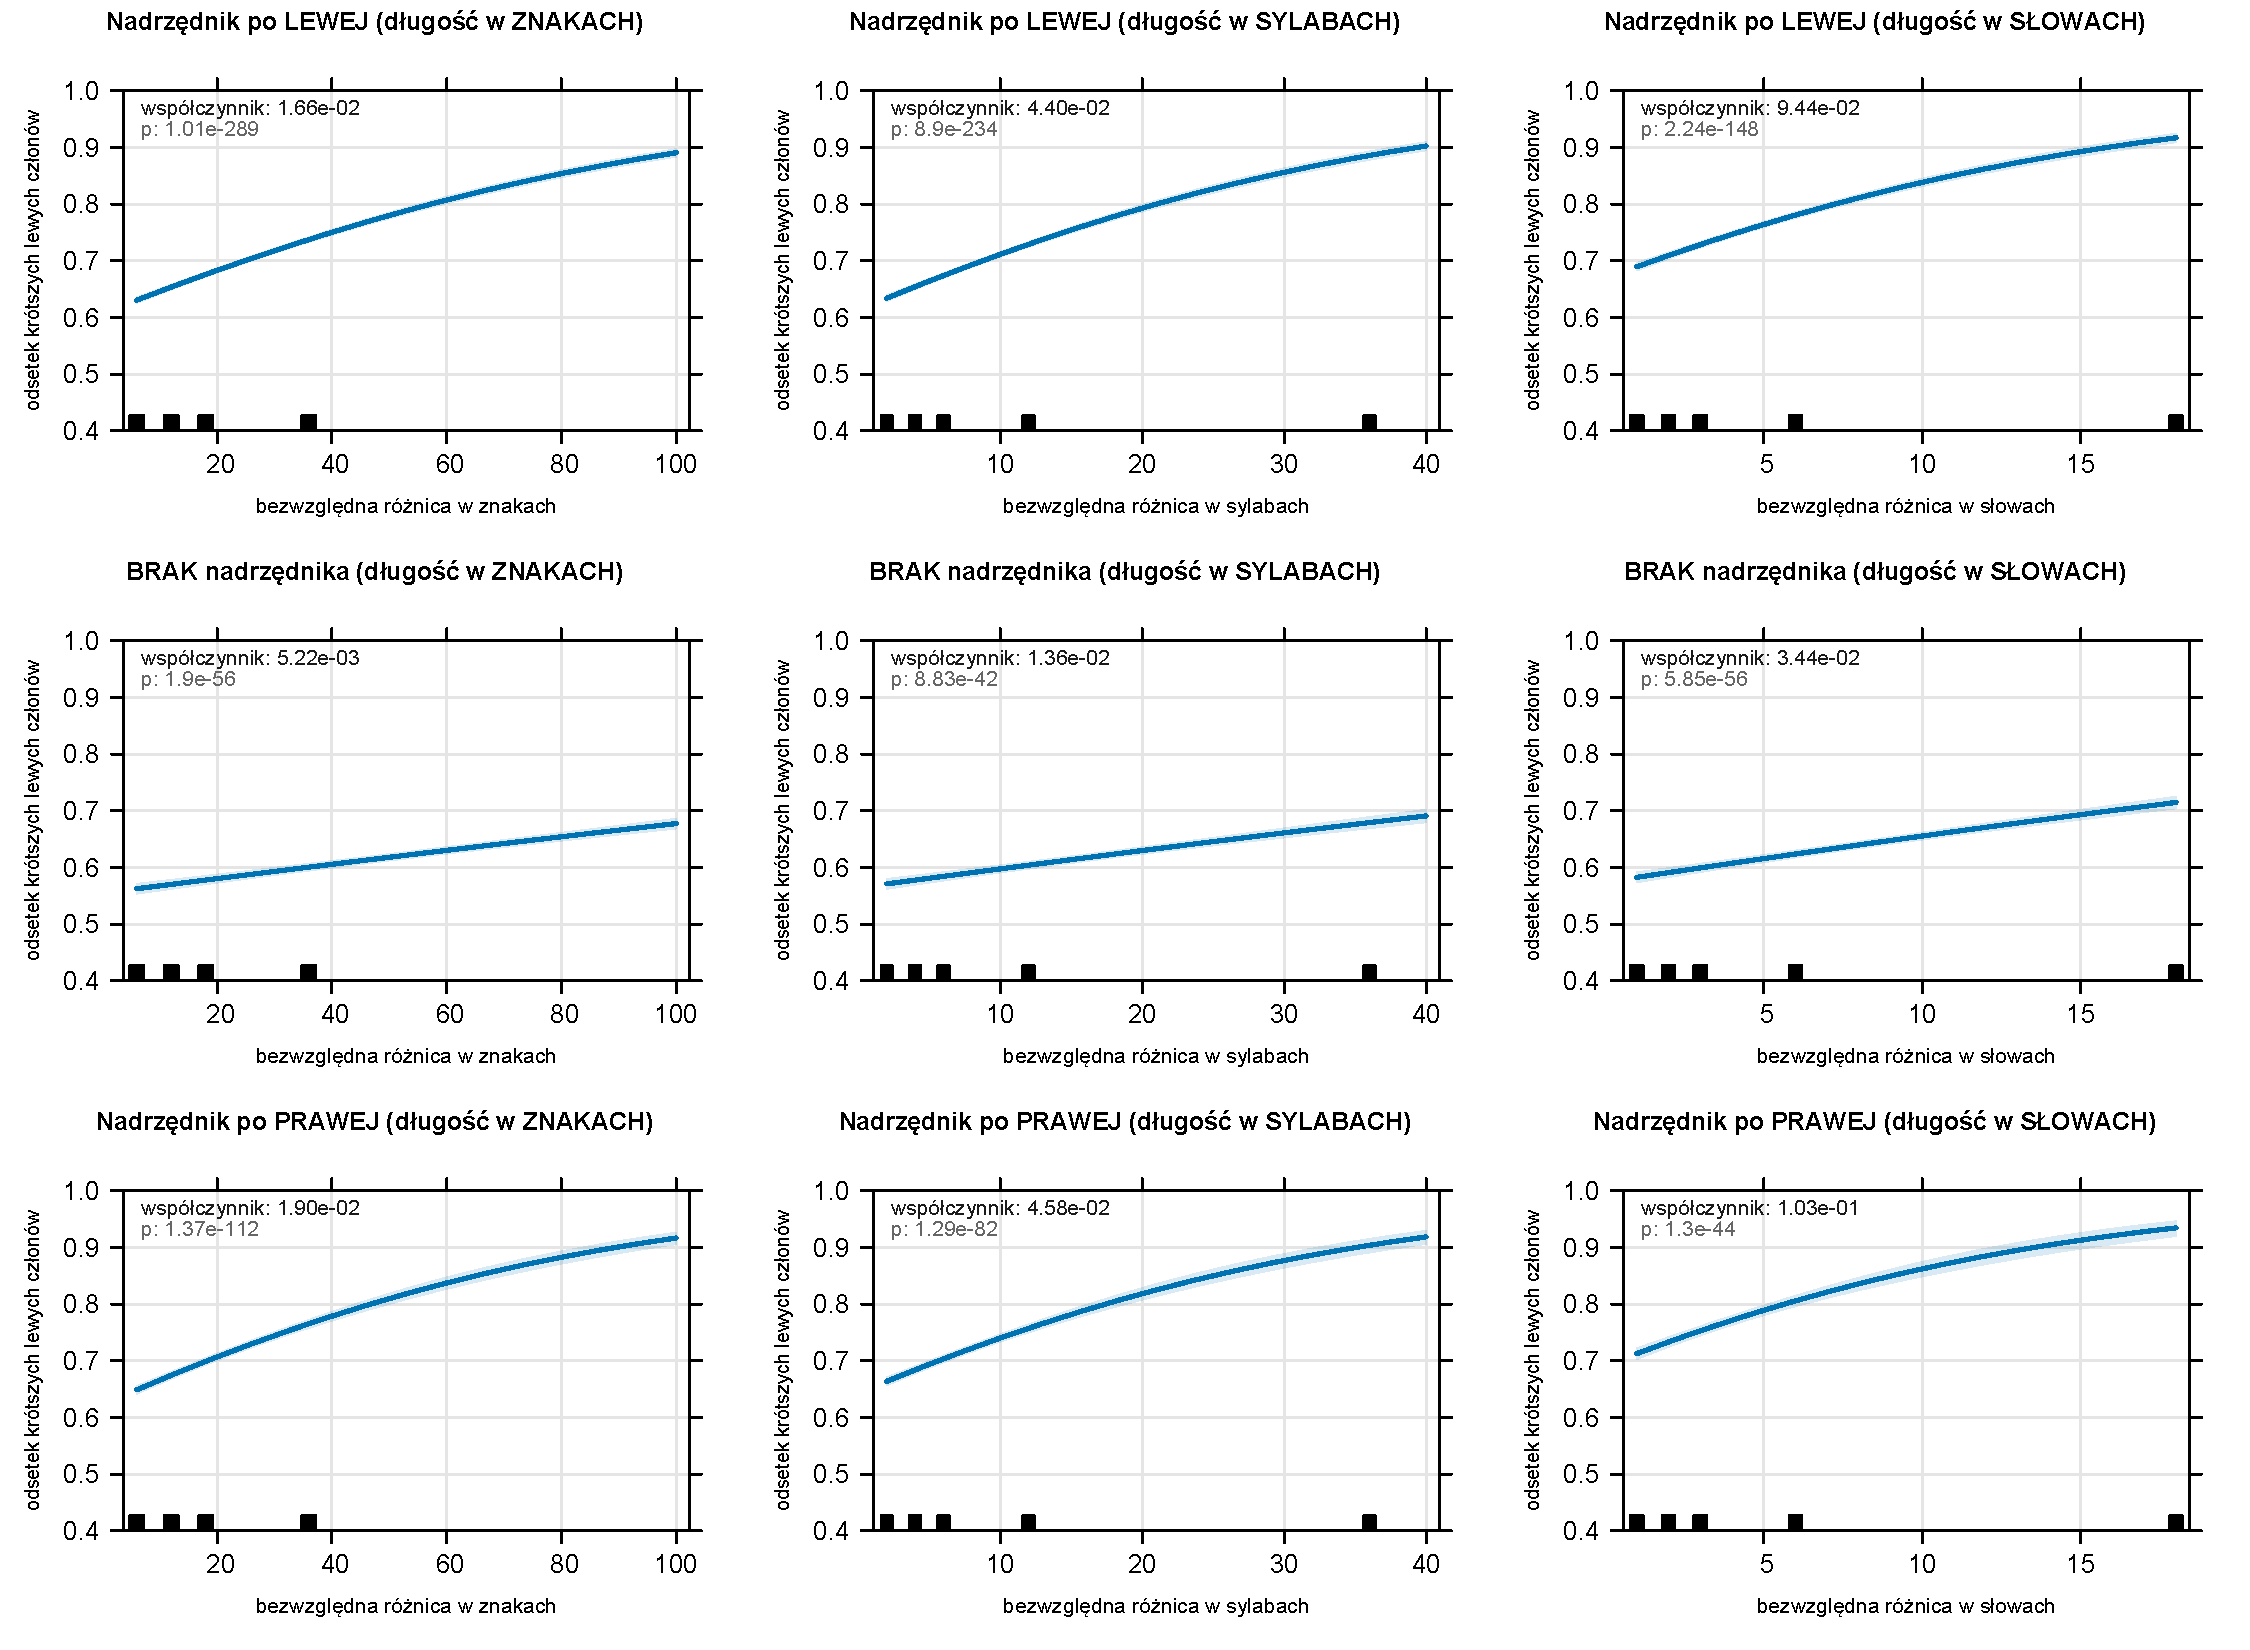
\includegraphics[scale=0.6]{German.pdf}
\caption{Różnica długości członów a występowanie krótszego członu po lewej stronie -- język \textbf{niemiecki}}
\label{fig:de}
\end{sidewaysfigure}

\newpage

\section{Języki finalne}

\begin{sidewaysfigure}
\centering
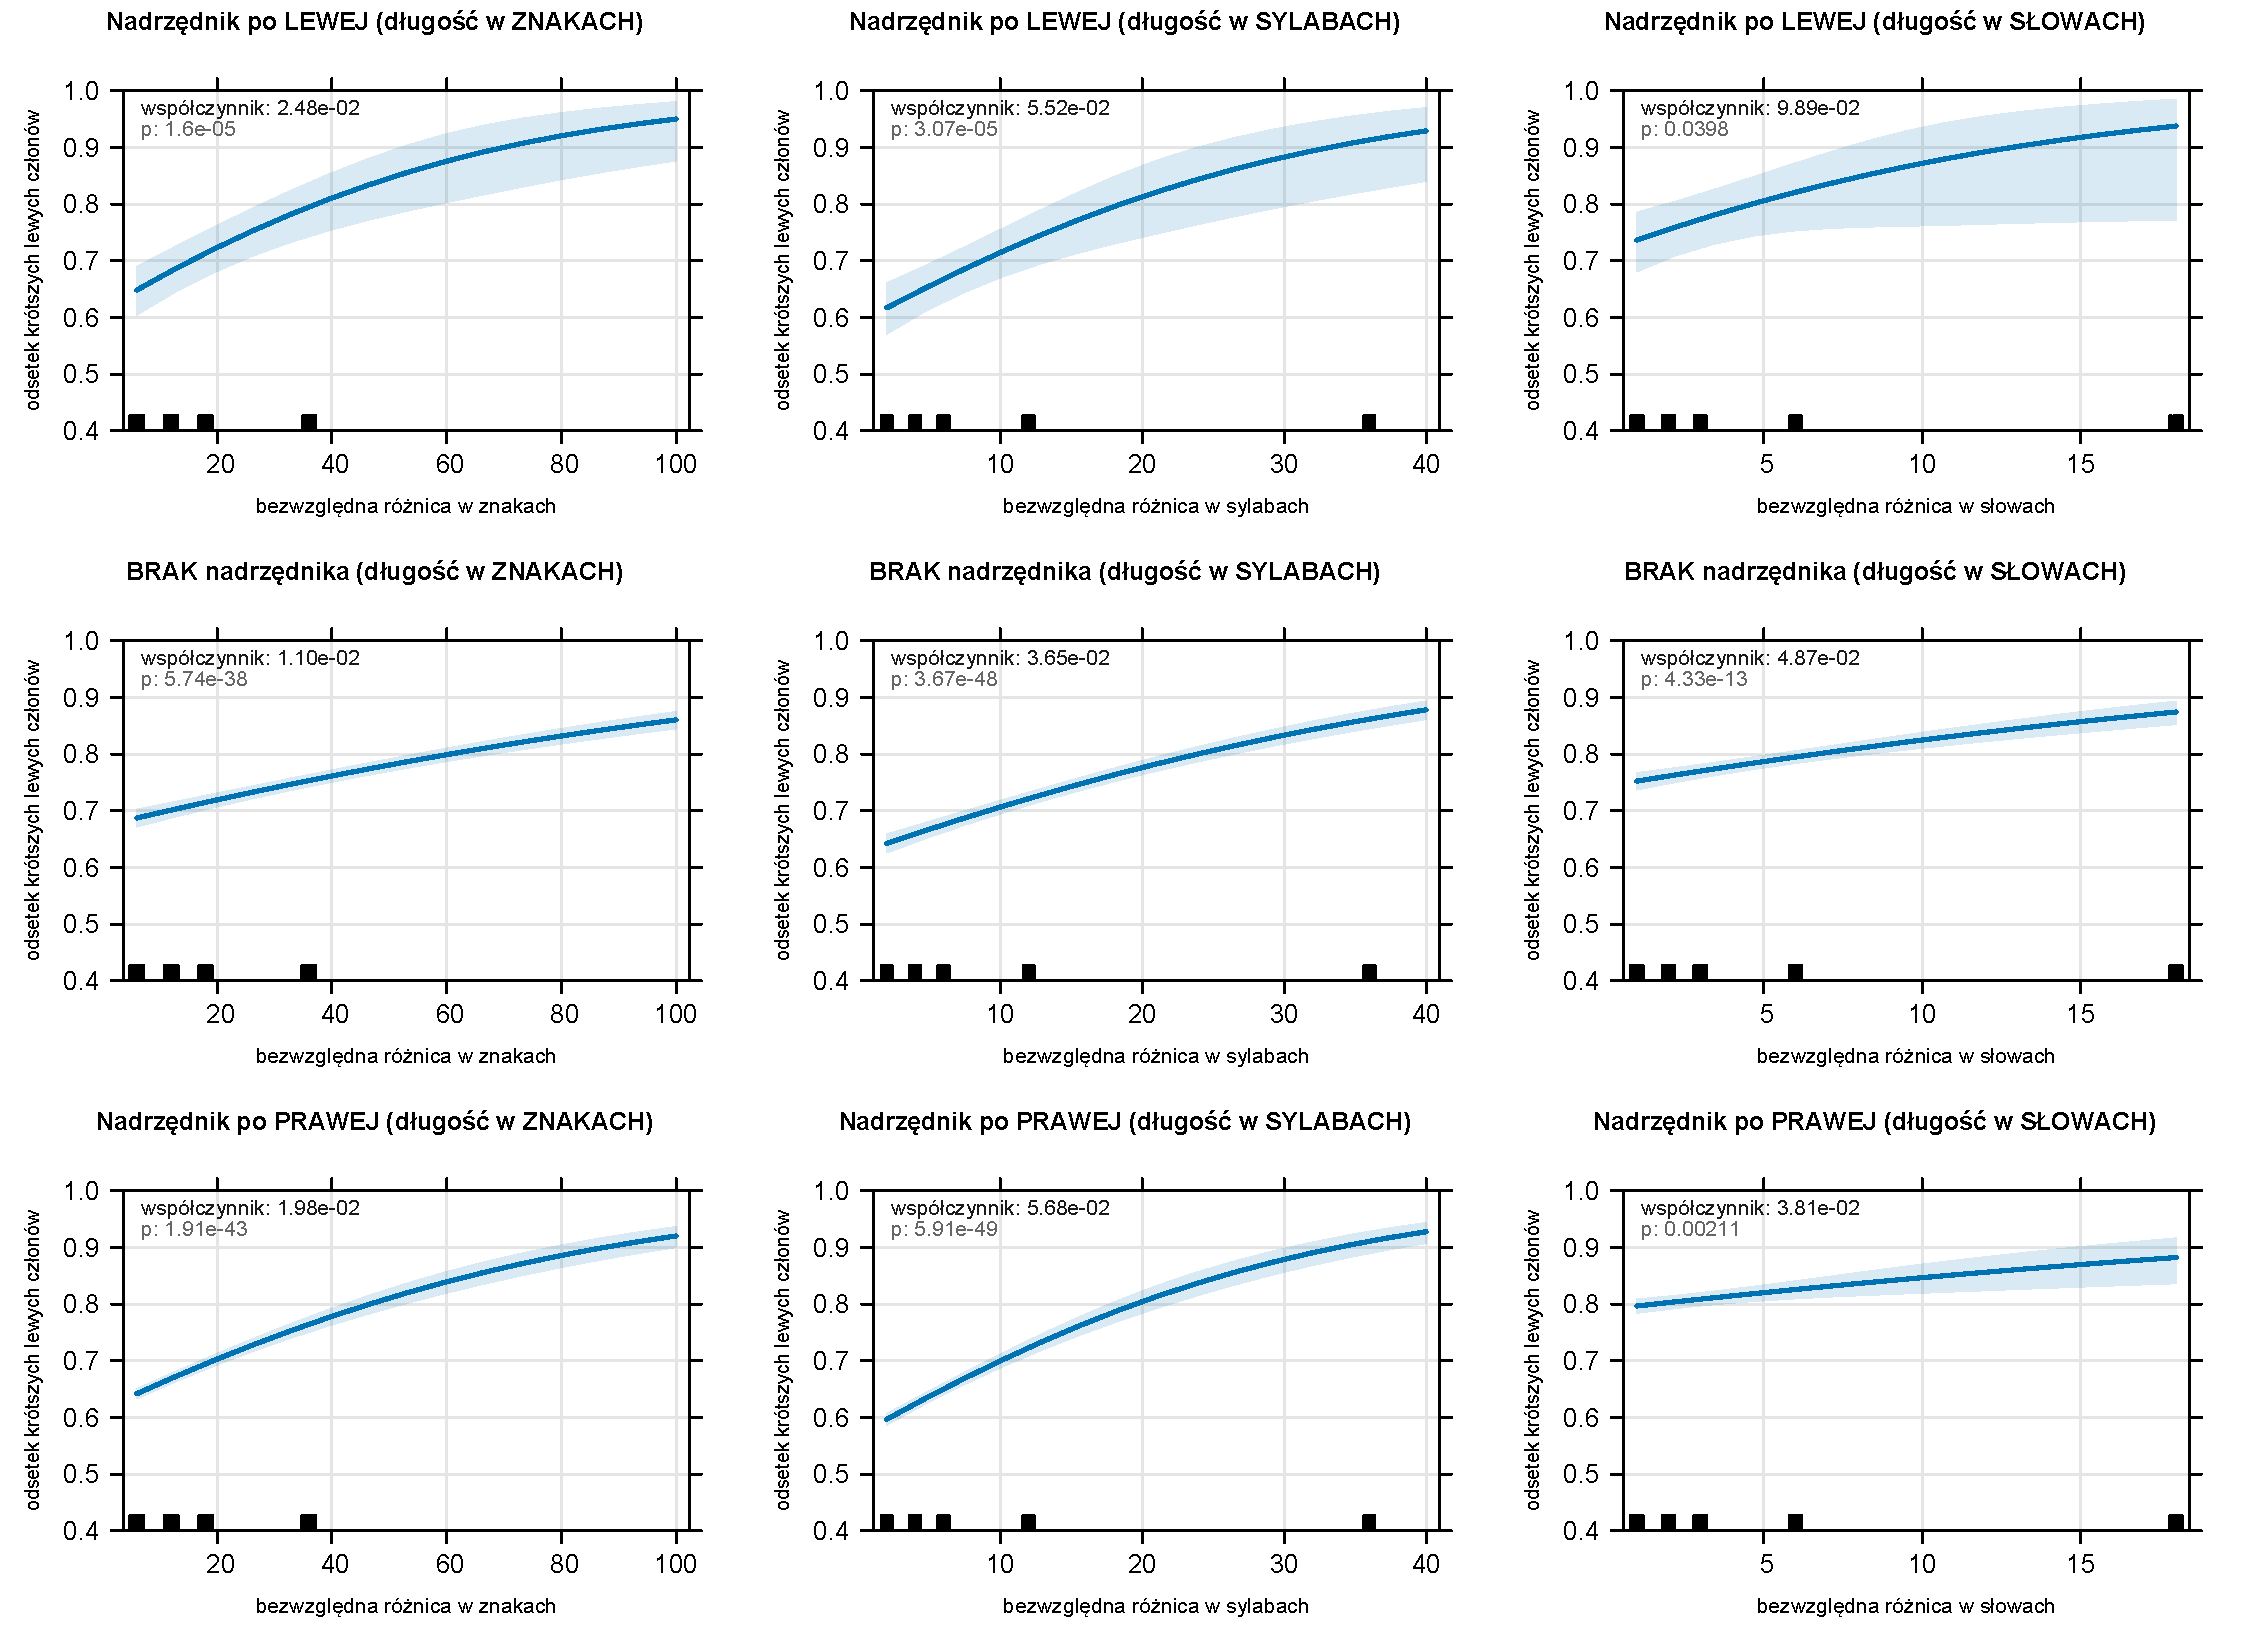
\includegraphics[scale=0.6]{Korean.pdf}
\caption{Różnica długości członów a występowanie krótszego członu po lewej stronie -- język \textbf{koreański}}
\label{fig:ko}
\end{sidewaysfigure}

\begin{sidewaysfigure}
\centering
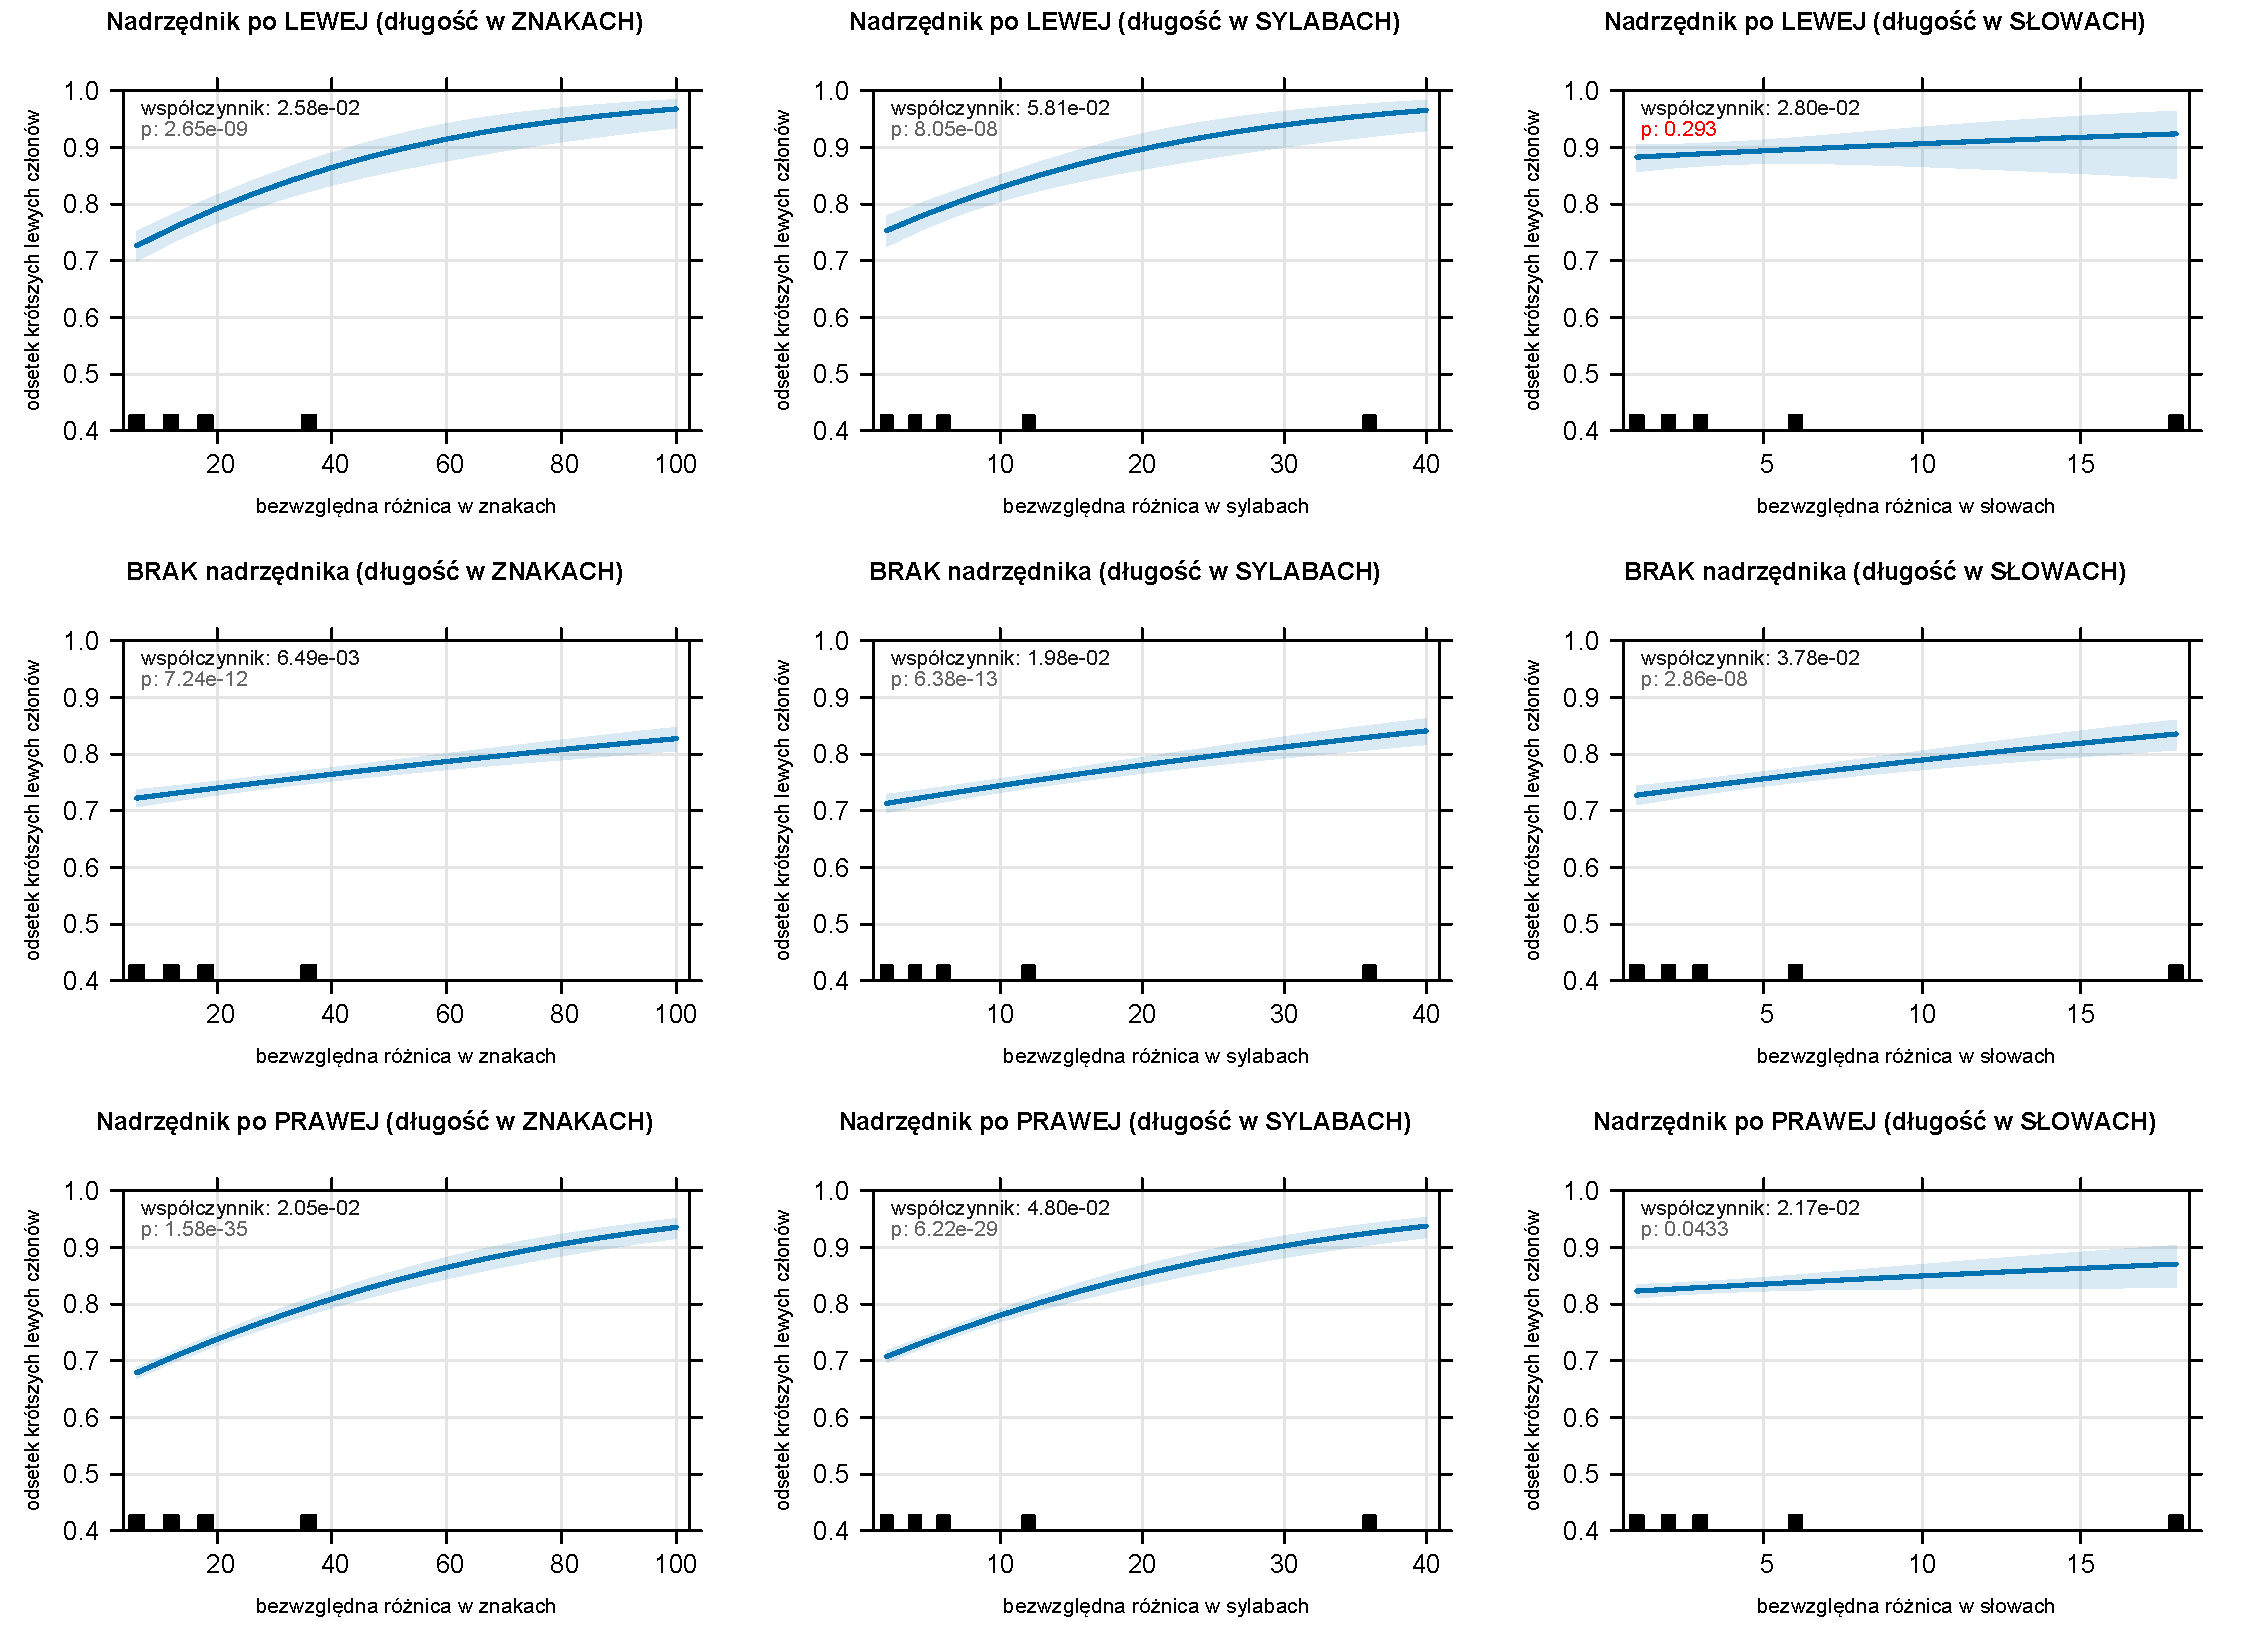
\includegraphics[scale=0.6]{Turkish.pdf}
\caption{Różnica długości członów a występowanie krótszego członu po lewej stronie -- język \textbf{turecki}}
\label{fig:tr}
\end{sidewaysfigure} % Wykresy - Różnica długości członów a pozycja krótszego członu

\bibliographystyle{apa-pl}
\bibliography{contents/references}

\end{document}
